\RequirePackage{ifthen}
\newboolean{longpage}
\setboolean{longpage}{false}
\ifthenelse{\boolean{longpage}}%
{\documentclass[10pt]{article}}%
{\documentclass[10pt]{book}}

\newboolean{printlabelname}
\setboolean{printlabelname}{false}
\ifthenelse{\boolean{printlabelname}}{\usepackage[notref,notcite]{showkeys}}{}
\usepackage{pdfpages}

\newboolean{colour}
\setboolean{colour}{true}


%% end detour
%\usepackage{amsmath}
\usepackage{xr}
\externaldocument{Math1560_ebook}

%%Page Size stuff

\newboolean{tabletsize}
\ifthenelse{\boolean{longpage}}% if longpage, tablet automatically false
{\setboolean{tabletsize}{false}}%% if not longpage, then set tablet
{\setboolean{tabletsize}{false}}

%% Layout for printed book through Amazon CreateSpace, perfect bound,
%% 8.5 x 11 paper size, 1in inner margin, 1/2in (roughly) outer margin

%% for regular sized pages
\ifthenelse{\boolean{longpage}}%
				{\usepackage[paperheight=20in,
				paperwidth=7in,%inner=1in,
				textheight=18in,textwidth=320pt%,marginparwidth=150pt,marginparsep=32pt
				]{geometry}}%
				%% else not long page; 
				{% not longpage
				\usepackage[paperheight=11in,paperwidth=8.5in,%
						inner=1in,textheight=9in,textwidth=320pt,marginparwidth=150pt,%
						marginparsep=32pt,bottom=1in,footskip=29pt]{geometry}}

\ifthenelse{\boolean{longpage}}%
{% longpage - do not make changes to the text height for exercises
\newcommand{\exercisegeometry}{%
\newgeometry{inner=72pt,outer=72pt,textheight=18in,%textwidth=320pt,
						marginparwidth=150pt,marginparsep=32pt}
															}
}% ends if longpage
{% not longpage - regular sized exercise sets
%%
%% the old size of exercises
%
%\newcommand{\exercisegeometry}{%
%\newgeometry{inner=72pt,%
						%outer=72pt,textheight=545pt,%textwidth=320pt,
						%marginparwidth=150pt,%
						%marginparsep=32pt,
						%}
															%}
%%
%% the new size of exercises
%%
\newcommand{\exercisegeometry}{%
\newgeometry{inner=72pt,%
						outer=72pt,textheight=9.25in,tmargin=.75in,%textwidth=320pt,
						marginparwidth=150pt,%
						marginparsep=32pt,footskip=29pt,
						%bottom=1in,
						}
															}
}% ends if/then/else longpage

\newcommand{\eendgeometry}{%
\newgeometry{inner=72pt,%
						outer=36pt,textheight=10in,%textwidth=320pt,
						marginparwidth=150pt,%
						marginparsep=32pt,
						%bottom=1in%,footskip=1.5in
						}%
													}

\newcommand{\prefacegeometry}{%
\newgeometry{inner=1in,textheight=9in,textwidth=320pt,marginparwidth=150pt,%
						marginparsep=32pt,bottom=1in,footskip=1.5in}
															}


\ifthenelse{\boolean{longpage}}{%
	\usepackage{everyshi}
	\textheight500cm
	\EveryShipout{%
	\pdfpagewidth=7in
	\pdfpageheight=\pagetotal
	\advance\pdfpageheight by 3in
	\advance\pdfpageheight by 2\topmargin
	\advance\pdfpageheight by \textheight
	\advance\pdfpageheight by -\pagegoal}
%%
	\newcounter{chapter}
	\newcommand{\chapter}{\refstepcounter{chapter}\Huge Chapter \thechapter \vskip 2\baselineskip\normalsize}
}{}


\usepackage{APEX_format}
%%%%
% Additional packages to support the book, not part of the APEX style.
%%%%
\usepackage{fancyhdr}
\usepackage{eso-pic}
\usepackage{lipsum}
\usepackage{units}
%\usepackage{pgfplots}
%\pgfplotsset{width=\marginparwidth+1pt,compat=1.3}
\usepackage[font=small]{caption}
%,justification=centering

%%%%
%% These are low level LaTeX commands that determine the 
%% look of the Chapter and Section headings.
%% Note the use in the chapter part of an external file
%% that contains graphics for each chapter start.
%%%%

%%%%
%% Commands for the header, utilizing the fancyhdr
%% (fancy header) package
%%%%

\pagestyle{fancy}
\fancyhead{}
%\fancyfoot{}
\renewcommand{\chaptermark}[1]{\markboth{\chaptername\ \thechapter\ \ \ \ {#1}}{}}
\renewcommand{\sectionmark}[1]{\markright{\thesection\ \ \ \  #1}}
\fancyhf{}         %Clears all header and footer fields, in preparation.
\renewcommand{\headrulewidth}{0pt}
\renewcommand{\footrulewidth}{0pt}

\ifthenelse{\boolean{longpage}}%
{}% end header of longpage
{% begin header/footer of not longpage
\fancyhfoffset[LE,RO]{\marginparwidth+\marginparsep}
%\fancyfoot[LE,RO]{\textbf{\thepage}} %Displays the page number in bold in the header,

\fancyfoot{}
\fancyfoot[LE]{\textbf{\thepage}}
\fancyfoot[RO]{\textbf{\thepage}}

%\fancyfoot[LE]{\begin{minipage}{\textwidth}%
%\noindent\hskip\marginparwidth\hskip\marginparsep\hskip-4pt\rule{\textwidth}{.4pt}
%\vskip.2\baselineskip
%\noindent\hskip\marginparwidth\hskip\marginparsep\hskip-4pt%
%Notes:
%\vskip 1.5in\textbf{\thepage}
%\end{minipage}} 

%\fancyfoot[RO]{\begin{minipage}{\textwidth+\marginparwidth+\marginparsep}%
%\rule{\textwidth-\marginparwidth-\marginparsep}{.4pt}
%\vskip.2\baselineskip
%Notes:
%\vskip 1.5in
%\hfill\textbf{\thepage}
%\end{minipage}}       


\fancyhead[LE]{\nouppercase{\leftmark}}
      %Displays the upper-level (chapter) information---
      % as determined above---in non-upper case in the header, 
      %to the right on even pages.
\fancyhead[RO]{\rightmark}
			%Displays the lower-level (section) information---as
      % determined above---in the header, to the left on odd pages.
      
}% End the ifthenelse{longpage}


\ifthenelse{\boolean{longpage}}% for changing the header
{% longpage
\newcommand{\exerciseheader}{}
\newcommand{\regularheader}{}
\newcommand{\endmatheader}{}
}% i.e, the above does nothing
{% now for a real change
\newcommand{\exerciseheader}{%
				\fancyhfoffset[LE,RO]{32pt}%
				\fancyfoot[LE]{\textbf{\thepage}}% 
				\fancyfoot[RO]{\textbf{\thepage}}
				\fancyhead{}% 
}

\newcommand{\regularheader}{%
\fancyhead[LE]{\nouppercase{\leftmark}}%
\fancyhead[RO]{\rightmark}%
%\fancyfoot[LE]{}
%\fancyfoot[RO]{}
\fancyfoot{}
\fancyfoot[LE]{\textbf{\thepage}}
\fancyfoot[RO]{\textbf{\thepage}}
%\fancyfoot[LE]{\begin{minipage}{\textwidth}%
%\noindent\hskip\marginparwidth\hskip\marginparsep\hskip-4pt\rule{\textwidth}{.4pt}
%\vskip.2\baselineskip
%\noindent\hskip\marginparwidth\hskip\marginparsep\hskip-4pt%
%Notes:
%\vskip 1.5in\textbf{\thepage}
%\end{minipage}} 

%\fancyfoot[RO]{\begin{minipage}{\textwidth+\marginparwidth+\marginparsep}%
%\rule{\textwidth-\marginparwidth-\marginparsep}{.4pt}
%\vskip.2\baselineskip
%Notes:
%\vskip 1.5in
%\hfill\textbf{\thepage}
%\end{minipage}}

\fancyhfoffset[LE,RO]{\marginparsep+\marginparwidth}
}

\newcommand{\qendheader}{%
		\fancyhead{}%
		\fancyfoot{}%
		}
}% ends if/then/else exercise/regular headers


%
%  Defining what the chapter titles look like
%

\newdimen\titleheight

\makeatletter
\def\@makechapterhead#1{%
  {\parindent \z@ \raggedright \reset@font
    {\Huge \thechapter: \scshape \textsc #1}
    \par\vskip 10\p@
    \hrule height 1pt
    \vskip 10\p@
  }}
%%  
%%%\makeatletter
%%\def\@makesectionhead#1{%
%%	 {\reset@font\LARGE\itshape\bfseries\strut #1 \thechapter.\thesection \ #1
%%	 }}

%%%%
%%
%%  For figures in the margin
%%
%%%%

%%\usepackage{wrapfig}
%%
%%\setlength{\marginparsep}{10pt}
%%\setlength{\wrapoverhang}{\marginparwidth}
%%\addtolength{\wrapoverhang}{\marginparsep}
%%
%%%\newenvironment{mfigure}[1]{%
%%%    \wrapfigure{#1}{0pt}%
%%%    \begin{minipage}{\marginparwidth}%
%%%    \centering%
%%%}{%
%%%    \end{minipage}%
%%%    \endwrapfigure%
%%%}


\ifthenelse{\boolean{longpage}}%
		{\newcommand{\mfigure}[5][]{%
		\vskip \baselineskip%
			\noindent\begin{minipage}{\textwidth}
  			\centering
  			\myincludegraphics{#5}
  			#1%
  			\captionsetup{type=figure}
	  		\caption{#3}\label{#4}
  		\end{minipage}
		}}
		{\newcommand{\mfigure}[5][]{%
		\ifthenelse{\isodd{\thepage}}%
			{\AddToShipoutPicture*{\put(427,\LenToUnit{#2\paperheight}){%
			\begin{minipage}{\marginparwidth}%
				\centering%
	  		\myincludegraphics[#1]{#5}%
  			\captionsetup{type=figure}%
  			%#1%
	  		\caption{#3}\label{#4}%
  		\end{minipage}}}}%
			{\AddToShipoutPicture*{\put(36,\LenToUnit{#2\paperheight}){%
			\begin{minipage}{\marginparwidth}%
			  \centering%
  			\myincludegraphics[#1]{#5}%
  			\captionsetup{type=figure}%
  			%#1%
	  		\caption{#3}\label{#4}%
  		\end{minipage}}}}%
		}}%

\ifthenelse{\boolean{longpage}}%
		{\newcommand{\mtable}[4]{
					\vskip \baselineskip%
					\noindent\begin{minipage}{\textwidth}
  					\centering\small
  					#4
  					\captionsetup{type=figure}
	  				\caption{#2}\label{#3}
  				\end{minipage}
  				\vskip\baselineskip}
  	}
		{\newcommand{\mtable}[4]{%
			\ifthenelse{\isodd{\thepage}}%
				{\AddToShipoutPicture*{\put(427,\LenToUnit{#1\paperheight}){%
					\begin{minipage}{\marginparwidth}%
  					\centering\small%
  					#4%
  					\captionsetup{type=figure}%
	  				\caption{#2}\label{#3}%
  				\end{minipage}}}}%
				{\AddToShipoutPicture*{\put(36,\LenToUnit{#1\paperheight}){%
					\begin{minipage}{\marginparwidth}%
 						 \centering\small%
 						 #4%
						  \captionsetup{type=figure}%
	  					\caption{#2}\label{#3}%
 					 \end{minipage}}}}%
		}}%

\ifthenelse{\boolean{longpage}}%
		{\newcommand{\mnote}[2]{%
					\hskip 25pt%
					\begin{minipage}{\marginparwidth}%
					\small%
					#2%
					\end{minipage}%
					\vskip\baselineskip%
		}%
		}%
		{\newcommand{\mnote}[2]{%
			\ifthenelse{\isodd{\thepage}}%
				{\AddToShipoutPicture*{\put(427,\LenToUnit{#1\paperheight}){%
					\begin{minipage}{\marginparwidth}
  					\small
  					#2
  				\end{minipage}}}}%
				{\AddToShipoutPicture*{\put(36,\LenToUnit{#1\paperheight}){%
					\begin{minipage}{\marginparwidth}
 						 \small
 						 #2
					\end{minipage}}}}
		}}

%\ifthenelse{\boolean{longpage}}%
		%{}
		%{\newcommand{\mfigurethree}[5][]{%
		%\ifthenelse{\isodd{\thepage}}%
			%{\AddToShipoutPicture*{\put(427,\LenToUnit{#2\paperheight}){%
			%\begin{minipage}{\marginparwidth}%
				%\centering%
	  		%\includemedia[#1]{\includegraphics{#5}}{#5.prc}%
  			%\captionsetup{type=figure}%
  			%%#1%
	  		%\caption{#3}\label{#4}%
  		%\end{minipage}}}}%
			%{\AddToShipoutPicture*{\put(36,\LenToUnit{#2\paperheight}){%
			%\begin{minipage}{\marginparwidth}%
			  %\centering%
  			%\includemedia[#1]{\includegraphics{#5}}{#5.prc}%
  			%\captionsetup{type=figure}%
  			%%#1%
	  		%\caption{#3}\label{#4}%
  		%\end{minipage}}}}%
		%}}%
		
		\newcommand{\mfigurethree}[6]{%
		\ifthenelse{\isodd{\thepage}}%
			{\AddToShipoutPicture*{\put(427,\LenToUnit{#3\paperheight}){%
			\begin{minipage}{\marginparwidth}%
				\centering%
				\ifthenelse{\boolean{in_threeD}}{% in 3D
	  		\includemedia[#1]{\includegraphics{#6_3D\colornamesuffix}}{#6_3D.prc}}%now not in 3D
				{\myincludegraphics[#2]{#6}}%
  			\captionsetup{type=figure}%
  			%#1%
	  		\caption{#4}\label{#5}%
  		\end{minipage}}}}%
			{\AddToShipoutPicture*{\put(36,\LenToUnit{#3\paperheight}){%
			\begin{minipage}{\marginparwidth}%
			  \centering%
  			\ifthenelse{\boolean{in_threeD}}{% in 3D
	  		\includemedia[#1]{\includegraphics{#6_3D\colornamesuffix}}{#6_3D.prc}}%now not in 3D
				{\myincludegraphics[#2]{#6}}%
  			\captionsetup{type=figure}%
  			%#1%
	  		\caption{#4}\label{#5}%
  		\end{minipage}}}}%
		}

%\AddToShipoutPicture{\ifthenelse{\ifodd{\thepage}}%
%{\put(10,10){\begin{tikzpicture}\draw (0,0) circle (5pt);\end{tikzpicture}}}%
%{\put(100,100){\begin{tikzpicture}\draw (0,0) circle (5pt);\end{tikzpicture}}}}%
%

%\AddToShipoutPictureBG{%
% \AtPageLowerLeft{\hspace{1cm}A small logo: \rule{2cm}{3cm}}}
% 
%}{\AddToShipoutPicture*{\put(36,\LenToUnit{#2\paperheight})}}%
%{%
%\begin{minipage}{\marginparwidth}
%  \centering
%  \includegraphics{#1}
%  \captionof{figure}{#3}
%  \end{minipage}}}
%\AddToShipoutPicture*{\put(\LenToUnit{.5\paperwidth},\LenToUnit{.75\paperheight}){%
%  \begin{minipage}{100pt}
%  \centering
%  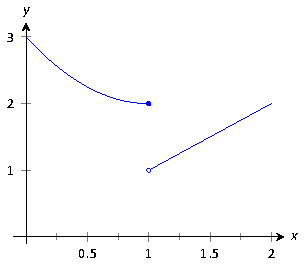
\includegraphics{test-figure2.pdf}
%  \captionof{figure}{Test caption}
%  \end{minipage}}}


%\newenvironment{mfigurefile}[2]{%
%\begin{tikzpicture}[remember picture,overlay]%
%\ifthenelse{\isodd{\thepage}}{\node [xshift=-36pt-.5\marginparwidth,yshift=#2\paperheight] at (current page.south east) }{\node [xshift=36pt+.5\marginparwidth,yshift=#2\paperheight] at (current page.south west) }%
%{\input{#1}};}%
%{\end{tikzpicture}%
%}

%\DeclareCaptionType{mytype}[Typename][List of mytype]


    
%%%%
%% End margin figure 
%%%%    
    

\newcommand{\bmx}[1]{\left[\hskip -3pt\begin{array}{#1} }
\newcommand{\emx}{\end{array}\hskip -3pt\right]}

\newcommand{\btz}{\begin{center}\begin{tikzpicture}}
\newcommand{\etz}{\end{tikzpicture}\end{center}}

\newcommand{\ds}{\displaystyle}

\newcommand{\fp}{\ensuremath{f\,'}}
\newcommand{\fpp}{\ensuremath{f\,''}}

\newcommand{\Fp}{\ensuremath{F\primeskip'}}
\newcommand{\Fpp}{\ensuremath{F\primeskip''}}

\newcommand{\yp}{\ensuremath{y\primeskip'}}
\newcommand{\gp}{\ensuremath{g\primeskip'}}

\newcommand{\dx}{\ensuremath{\Delta x}}
\newcommand{\dy}{\ensuremath{\Delta y}}
%\newcommand{\dz}{\ensuremath{\Delta z}}
\newcommand{\ddz}{\ensuremath{\Delta z}}

\newcommand{\thet}{\ensuremath{\theta}}
\newcommand{\norm}[1]{\ensuremath{||\ #1\ ||}}
\newcommand{\vnorm}[1]{\ensuremath{\norm{\vec #1}}}
\newcommand{\snorm}[1]{\ensuremath{\left|\left|\ #1\ \right|\right|}}
\newcommand{\la}{\left\langle}
\newcommand{\ra}{\right\rangle}
\newcommand{\dotp}[2]{\ensuremath{\vec #1 \cdot \vec #2}}
\newcommand{\proj}[2]{\ensuremath{\text{proj}_{\,\vec #2}{\,\vec #1}}}
\newcommand{\crossp}[2]{\ensuremath{\vec #1 \times \vec #2}}
\newcommand{\veci}{\ensuremath{\vec i}}
\newcommand{\vecj}{\ensuremath{\vec j}}
\newcommand{\veck}{\ensuremath{\vec k}}
\newcommand{\vecu}{\ensuremath{\vec u}}
\newcommand{\vecv}{\ensuremath{\vec v}}
\newcommand{\vecw}{\ensuremath{\vec w}}
\newcommand{\vecx}{\ensuremath{\vec x}}
\newcommand{\vecy}{\ensuremath{\vec y}}
\newcommand{\vrp}{\ensuremath{\vec r\, '}}
\newcommand{\vsp}{\ensuremath{\vec s\, '}}
\newcommand{\vrt}{\ensuremath{\vec r(t)}}
\newcommand{\vst}{\ensuremath{\vec s(t)}}
\newcommand{\vvt}{\ensuremath{\vec v(t)}}
\newcommand{\vat}{\ensuremath{\vec a(t)}}
\newcommand{\px}{\ensuremath{\partial x}}
\newcommand{\py}{\ensuremath{\partial y}}
\newcommand{\pz}{\ensuremath{\partial z}}
\newcommand{\pf}{\ensuremath{\partial f}}
\newcommand{\underlinespace}{\underline{\phantom{xxxxxx}}}

\newcommand{\mathN}{\ensuremath{\mathbb{N}}}

\newcommand{\zerooverzero}{\ensuremath{\ds \raisebox{8pt}{\text{``\ }}\frac{0}{0}\raisebox{8pt}{\text{\ ''}}}}


\newcommand{\myrule}{\rule[-4pt]{0pt}{13pt}}
\newcommand{\mmrule}{\rule[-10pt]{0pt}{15pt}}
\newcommand{\myds}{\ds\mmrule}
\newcommand{\deriv}[2]{\ensuremath{\myds\frac{d}{dx}\left(#1\right)=#2}}
\newcommand{\myint}[2]{\ensuremath{\myds\int #1\ dx=} \ensuremath{\ds #2}}

\DeclareMathOperator{\sech}{sech}
\DeclareMathOperator{\csch}{csch}

\newcommand{\sword}[1]{\textbf{#1}}

\newcommand{\primeskip}{\hskip.75pt}

%%%% Begin Header TikZ

%  Some TiKZ  shortcuts to help make drawing 3D vectors faster.
%

\newcommand{\plotlinecolor}{blue}

%
% Draw x and y tick marks
%
\newcommand{\drawxticks}[1]
{\foreach \x in {#1}
		{\draw  (\x,-.1)--(\x,.1);
			};
}
\newcommand{\drawyticks}[1]
{\foreach \x in {#1}
		{\draw  (-.1,\x)--(.1,\x);
			};
}

\newcommand{\drawxlines}[3]
{\draw[<->] (#1,0) -- (#2,0) node [right] {$x$};
\foreach \x in {#3}
		{\draw  (\x,-.1)--(\x,.1);
			};
}

\newcommand{\drawylines}[3]
{\draw[<->] (0,#1) -- (0,#2) node [above] {$y$};
\foreach \x in {#3}
		{\draw  (-.1,\x)--(.1,\x);
			};
}

\newcommand{\drawxlabels}[1]
{\foreach \x in {#1}
		{\draw  (\x,-.1) node [below] {\scriptsize $\x$};
		};
}

\newcommand{\drawylabels}[1]
{\foreach \x in {#1}
		{\draw  (-.1,\x) node [left] {\scriptsize $\x$};
		};
}

%% draw a box of margin width size to see if figure is properly contained within
\newcommand{\marginsizebox}{\draw (0,0)--(\marginparwidth,0)--(\marginparwidth,3)--(0,3)--cycle;}

%%%%
%%%%

\newcommand{\asyouread}[1]{\begin{tikzpicture}
\ifthenelse{\boolean{in_color}}{\node [preaction={fill=black,opacity=.5,transform canvas={xshift=1mm,yshift=-1mm}}, right color=blue!80!black!30, left color=blue!80] at (0,0) {\textcolor{white}{\textsf{\textit{AS YOU READ $\ldots$}}}};}
{\node [preaction={fill=black,opacity=.5,transform canvas={xshift=1mm,yshift=-1mm}}, right color=black!30, left color=black!10] at (0,0) {\textcolor{white}{\textsf{\textit{AS YOU READ $\ldots$}}}};}
\end{tikzpicture}
\begin{enumerate}
#1
\end{enumerate}
\vskip 20pt}

%%%%
%%  A new figure environment, trying to fix the float problem.
%%
%%%%

\newcounter{myfigurecounter}[chapter]
\renewcommand\themyfigurecounter{\thechapter.\arabic{myfigurecounter}}
\newenvironment{myfigure}{\refstepcounter{myfigurecounter}}{}
\newcommand{\mycaption}[1]{%
\begin{center}%
\vskip -1.5\baselineskip
\begin{tikzpicture}%
\draw (0,0) node [text width=\textwidth,align=center] {Figure \themyfigurecounter: #1};%
\end{tikzpicture}%
\end{center}%
}
\usepackage{pgfplots}
\pgfplotsset{compat=1.8}
\usepackage{pdfpages}


\ifthenelse{\boolean{xetex}}%
	{\sffamily
	%%\usepackage{fontspec}
	\usepackage{mathspec}
	\setallmainfonts[Mapping=tex-text]{Calibri}
	\setmainfont[Mapping=tex-text]{Calibri}
	\setsansfont[Mapping=tex-text]{Calibri}
	\setmathsfont(Greek){[cmmi10]}}
	{\usepackage[sfdefault,lf]{carlito}
	%% The 'lf' option for lining figures
	%% The 'sfdefault' option to make the base font sans serif
	\usepackage[T1]{fontenc}
	\renewcommand*\oldstylenums[1]{\carlitoOsF #1}}
	
	\ifthenelse{\boolean{luatex}}%
	{\sffamily
	\usepackage{fontspec}
	\usepackage{unicode-math}
	\usepackage{mathspec}
	\setallmainfonts[Mapping=tex-text]{Calibri}
	\setmainfont{Calibri}
	\setsansfont[Mapping=tex-text]{Calibri}
	\setmathfont[range=\mathup]{Calibri}
	\setmathfont[range=\mathit]{Calibri Italic}
	}
	{}

\makeindex

%%%\tracingonline=1
\begin{document}
%\printexercisenames
\printincolor
%\printinblackandwhite
%\printallanswers

%
%%%%%%%%%%
%%%
%%%  Set criteria for the format of the book.
%%%  This supercedes anything set in the Text_Header.
%%%
%%%%%%%%%%



%\printinblackandwhite

%\printexercisenames

%\nodrawexamplelines

%\printallanswers


\normalem



%%%\pagenumbering{roman}

%%%%%%
%%%		For editing purposes, block comment down to 
%%%		the next mark
%%%%%%

%%%%\input{cover/front_cover_in_text}
%%%%\clearpage
%%%%\thispagestyle{empty}
\frontmatter
%%%%
%%%%\title{\textsc{Fundamentals of Matrix Algebra}\\
%%%%{\small Version 2.1011}}
%%%%\author{Gregory N. Hartman, Ph.D.}
%%%%\date{}

\vspace*{\stretch{.5}}

\hskip 125pt\begin{minipage}{\textwidth}
\begin{flushright}

\textsc{{\Huge Math 2560 Calculus II}} \\

%\textsl{Third Edition}, 
{\large University of Lethbridge}\\

{A version of the \apex\ Calculus textbook edited by Sean Fitzpatrick}

\bigskip

\Large
%\vspace{1in}

Gregory Hartman, Ph.D.

\emph{\small Department of Applied Mathematics}

\emph{\small Virginia Military Institute}\vskip15pt

Ji{\v r}\'i Lebl, Ph.D.

\emph{\small Department of Mathematics}

\emph{\small University of Oklahoma}

\parbox{200pt}{\textit{Contributing Authors}}\hskip 2cm \phantom{.}

Troy Siemers, Ph.D.

\emph{\small Department of Applied Mathematics}

\emph{\small Virginia Military Institute}\vskip 15pt

Brian Heinold, Ph.D.

\emph{\small Department of Mathematics and Computer Science}

\emph{\small Mount Saint Mary's University}\vskip 15pt

Dimplekumar Chalishajar, Ph.D.

\emph{\small Department of Applied Mathematics}

\emph{\small Virginia Military Institute}\vskip 25pt



\parbox{200pt}{\textit{Editor}}\hskip 2cm \phantom{.}
%\textit{Editor}\hskip 7cm\phantom{.}

Jennifer Bowen, Ph.D.

\emph{\small Department of Mathematics and Computer Science}

\emph{\small The College of Wooster}


\normalsize
\end{flushright}
\end{minipage}

\vspace{\stretch{1}}


\thispagestyle{empty}
\clearpage

\vspace*{\stretch{5}}
\noindent\hskip -1in\begin{minipage}{2in}
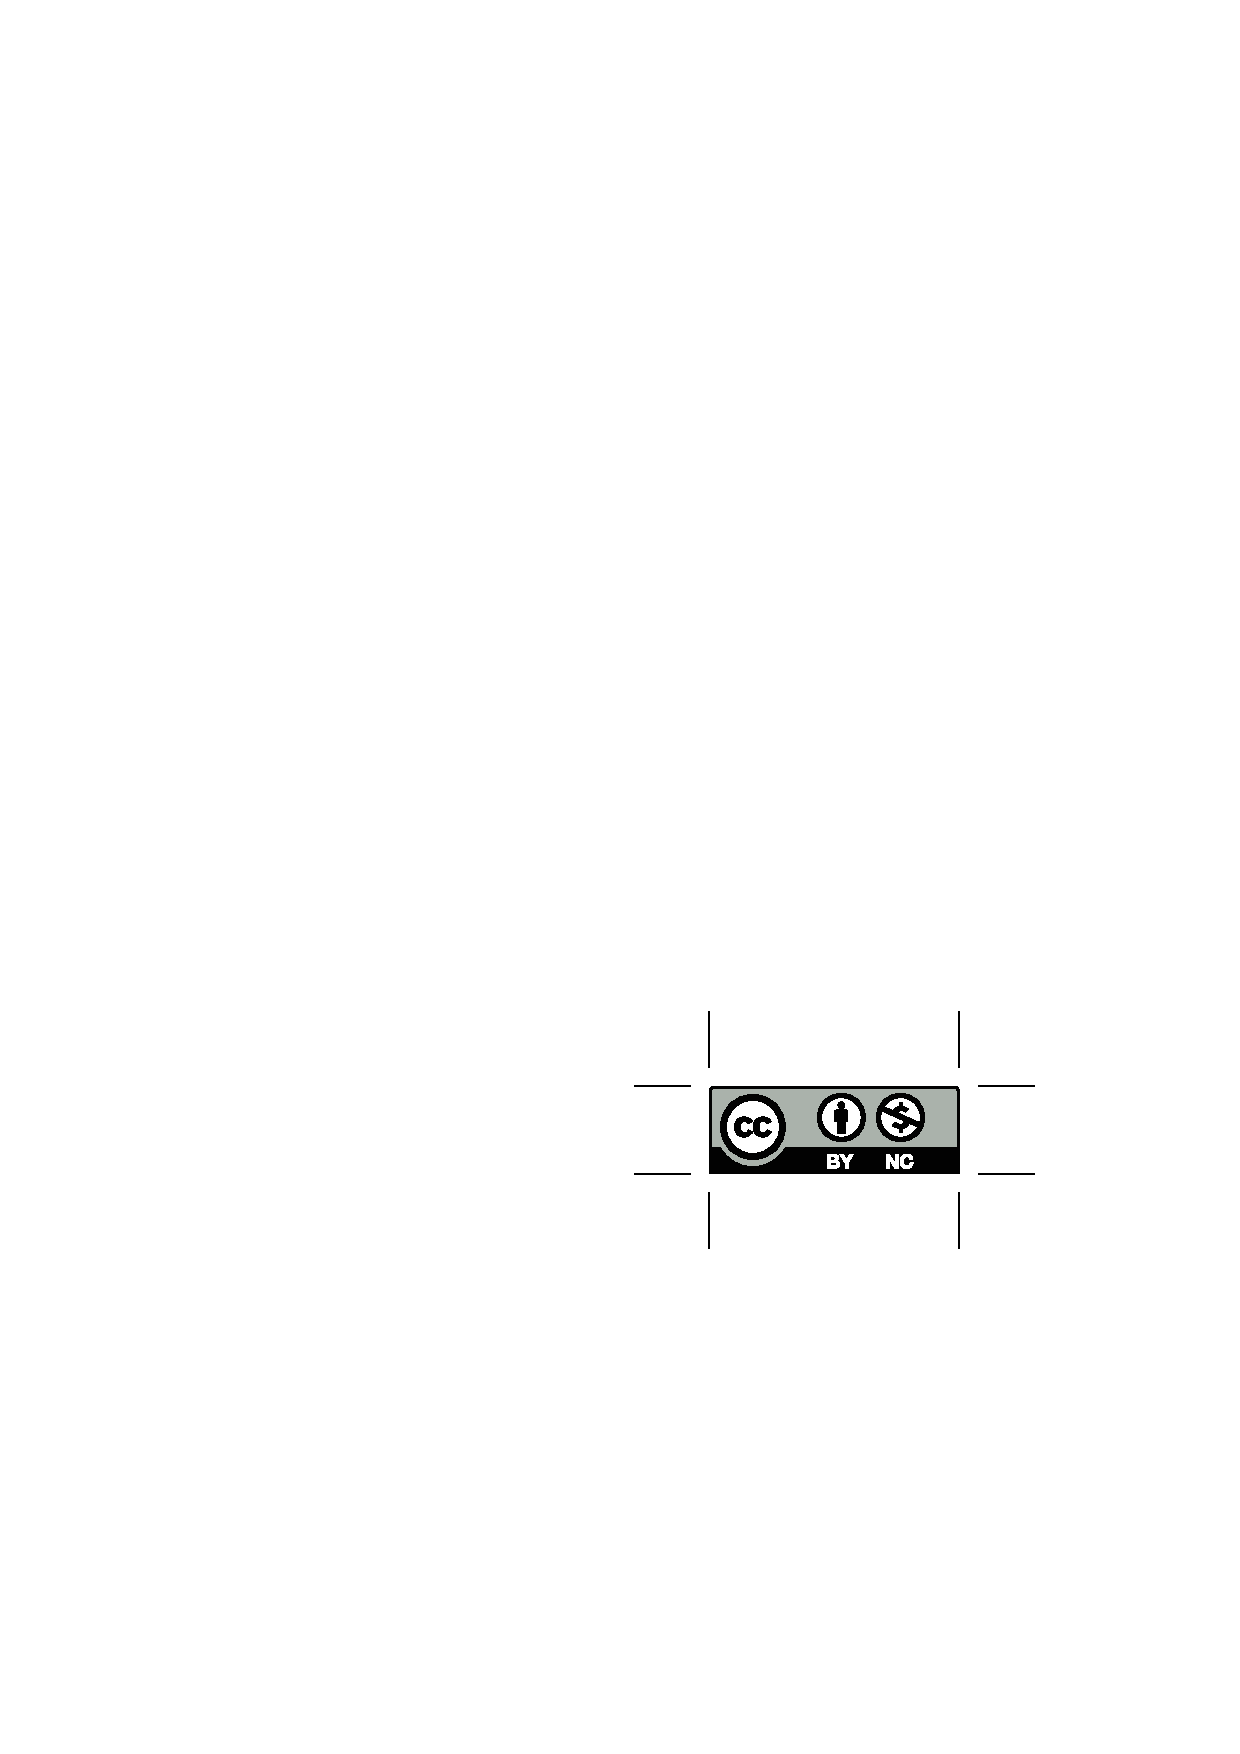
\includegraphics{text/by-nc} 
\end{minipage}
\begin{minipage}{3in}
\noindent Copyright \copyright\ 2015 Gregory Hartman

Licensed to the public under Creative Commons Attribution-Noncommercial 4.0 International Public License
\end{minipage}

\bigskip

\bigskip

Except Chapter 4 (Differential Equations) 

\bigskip

\bigskip

\noindent\hskip -1in\begin{minipage}{2in}

\includegraphics[width=1.7in]{figures/license} 
\end{minipage}
\begin{minipage}{3in}
\noindent Copyright \copyright 2008--2014 Ji{\v r}\'i Lebl

This work is licensed under the Creative Commons
Attribution-Non\-commercial-Share Alike 3.0 United States License. 
\end{minipage}

\bigskip

\bigskip

\noindent\hskip-1in\begin{minipage}{2in}

\includegraphics[width=1.7in]{figures/license}
\end{minipage}
\begin{minipage}{3.3in}
This version of the text was assembled and edited by Sean Fitzpatrick, University of Lethbridge, November 2015, revised most recently in April 2017. 

This work is licensed under the Creative Commons Attribution-Noncommercial-ShareAlike 4.0 International Public License
\end{minipage}
\vspace{\stretch{1}} 
\thispagestyle{empty}
\clearpage


%\cleardoublepage
%%%%\phantomsection
%%%%\input{text/thanks}
%%%%\addcontentsline{toc}{chapter}{Thanks} 
%%%%\clearpage{\pagestyle{empty}\cleardoublepage}

%%%%\phantomsection
%%%%
\addtocontents{toc}{\protect\thispagestyle{empty}}
\addtocontents{toc}{\protect\enlargethispage\baselineskip}
\addcontentsline{toc}{chapter}{Table of Contents}
\tableofcontents
\clearpage{\pagestyle{empty}\cleardoublepage}


\phantomsection
\prefacegeometry
\addcontentsline{toc}{chapter}{Preface}
\thispagestyle{empty}
\Huge
\noindent {\bf \textsc{Preface}}\\
\normalsize

This document is an attempt to provide a custom textbook that covers the entire curriculum (as of September 2017) for the course Math 2560 (Calculus II) at the University of Lethbridge at minimal cost to the student.



Most of this textbook is adapted from the \textit{APEX Calculus} textbook project, which originated in the Department of Applied Mathematics at the Virginia Military Institute. (See \href{http://www.apexcalculus.com}{apexcalculus.com}.) On the following page you'll find the original preface from their text, which explains their project in more detail. They have produced calculus textbook that is \textbf{free} in two regards: it's free to you, the student, in the sense that you can download the PDF from their website at no cost, and do with it as you wish (share it, print it, etc.) It's also free in the sense of being an \textit{open source} textbook: the authors have made all the files needed to produce the textbook freely available, and allow others (such as myself) to edit the text to suit the needs of various courses (such as Math 2560).

What's even better is that the textbook is of remarkably high production quality: unlike many free texts, it is polished and professionally produced, with graphics on almost every page, and a large collection of exercises (with selected answers!). If you're using the electronic version of the textbook, you'll even find that some of the graphics (those of 3D images) are interactive! Clicking on an image allows you to rotate it, and zoom in or out, to get a better understanding of the geometry involved. (This feature is only supported in Acrobat Reader, and not other PDF readers.)

Since Math 2560 includes content on differential equations, but the APEX Calculus textbook does not, I've also relied on the text \textit{Notes on Diffy Qs: Differential Equations for Engineers}, by Ji\v{r}\'i Lebl. (See \href{http://www.jirka.org/diffyqs}{jirka.org/diffyqs}.) This is another open source textbook that is free to use and adapt as needed. I have borrowed the first chapter of this text, and included it as a chapter in the APEX Calculus textbook, to provide you with a single textbook for the course. The integration is not entirely seamless: although I made changes to the formatting of the differential equations chapter so that it agrees in appearance with the rest of the textbook, I have not made any changes to Ji\v{r}\'{i}'s writing style, which is more conversational and familiar than the rest of the text. I felt it was more appropriate to preserve the voice of the original author.

I hope that you find this textbook useful. If you find any errors, or if you have any suggestions as to how the material could be better arranged or presented, please let me know. (The beauty of the open source textbook is that it can be edited at any time!)

\vspace{1in}

\begin{flushright}
Sean Fitzpatrick\\
Department of Mathematics and Computer Science\\
University of Lethbridge\\
April, 2017
\end{flushright}

\newpage

\Huge
\noindent {\bf \textsc{Preface to APEX Calculus}}\\
\large
\emph{A Note on Using this Text}
\vskip 2\baselineskip
\normalsize

Thank you for reading this short preface. Allow us to share a few key points about the text so that you may better understand what you will find beyond this page.

This text is Part II of a three--text series on Calculus. The first part covers material taught in many ``Calc 1'' courses: limits, derivatives, and the basics of integration, found in Chapters 1 through 6.1. The second text covers material often taught in ``Calc 2:'' integration and its applications, along with an introduction to sequences, series and Taylor Polynomials, found in Chapters 5 through 8. The third text covers topics common in ``Calc 3'' or ``multivariable calc:'' parametric equations, polar coordinates, vector--valued functions, and functions of more than one variable, found in Chapters 9 through 13. All three are available separately for free at \texttt{\href{http://www.vmi.edu/APEX}{www.vmi.edu/APEX}}. These three texts are intended to work together and make one cohesive text, \textit{APEX Calculus}, which can also be downloaded from the website. 

Printing the entire text as one volume makes for a large, heavy, cumbersome book. One can certainly only print the pages they currently need, but some prefer to have a nice, bound copy of the text. Therefore this text has been split into these three manageable parts, each of which can be purchased for under \$15 at \href{http://amazon.com}{Amazon.com}. 

A result of this splitting is that sometimes a concept is said to be explored in an ``earlier/later section,'' though that section does not actually appear in this particular text. Also, the index makes reference to topics, and page numbers, that do not appear in this text. This is done intentionally to show the reader what topics are available for study.  Downloading the .pdf of \textit{APEX Calculus} will ensure that you have all the content.\\ 
%material is referenced that is not contained in the present text. The context should make it clear whether the ``missing'' material is in the \textit{Calculus I} or \textit{Calculus III} portion. Downloading the appropriate .pdf, or the whole \textit{APEX Calculus} .pdf, will give access to these topics.
  %For instance, in this text, ``Theorem 20'' may be mentioned, although Theorem 20 is only presented in Part I. To minimize confusion, theorems, definitions and key ideas are referenced by their title or subject matter, not their number.

%The current publisher of this text does not allow one text to be split across multiple volumes, with continuity of chapters and page numberings. This is the one drawback of the current publishing model that has many advantages, highlighted below. Because of this, there are a few peculiarities 

\noindent\textbf{\large For Students: How to Read this Text}\\

Mathematics textbooks have a reputation for being hard to read. High--level mathematical writing often seeks to say much with few words, and this style often seeps into texts of lower--level topics. This book was written with the goal of being easier to read than many other calculus textbooks, without becoming too verbose. 

Each chapter and section starts with an introduction of the coming material, hopefully setting the stage for ``why you should care,'' and ends with a look ahead to see how the just--learned material helps address future problems. 

\textit{Please read the text;} it is written to explain the concepts of Calculus. There are numerous examples to demonstrate the meaning of definitions, the truth of theorems, and the application of mathematical techniques. When you encounter a sentence you don't understand, read it again. If it still doesn't make sense, read on anyway, as sometimes confusing sentences are explained by later sentences.

\textit{You don't have to read every equation.} The examples generally show ``all'' the steps needed to solve a problem. Sometimes reading through each step is helpful; sometimes it is confusing. When the steps are illustrating a new technique, one probably should follow each step closely to learn the new technique. When the steps are showing the mathematics needed to find a number to be used later, one can usually skip ahead and see how that number is being used, instead of getting bogged down in reading how the number was found.

\textit{Most proofs have been omitted.} In mathematics, \textit{proving} something is always true is extremely important, and entails much more than testing to see if it works twice. However, students often are confused by the details of a proof, or become concerned that they should have been able to construct this proof on their own. To alleviate this potential problem, we do not include the proofs to most theorems in the text. The interested reader is highly encouraged to find proofs online or from their instructor. In most cases, one is very capable of understanding what a theorem \textit{means} and \textit{how to apply it} without knowing fully \textit{why} it is true.
\\

\thispagestyle{empty}
\noindent\textbf{\large Interactive, 3D Graphics}\\

New to Version 3.0 is the addition of interactive, 3D graphics in the .pdf version. Nearly all graphs of objects in space can be rotated, shifted, and zoomed in/out so the reader can better understand the object illustrated. 

As of this writing, the only pdf viewers that support these 3D graphics are Adobe Reader \& Acrobat (and only the versions for PC/Mac/Unix/Linux computers, not tablets or smartphones). To activate the interactive mode, click on the image. Once activated, one can click/drag to rotate the object and use the scroll wheel on a mouse to zoom in/out. (A great way to investigate an image is to first zoom in on the page of the pdf viewer so the graphic itself takes up much of the screen, then zoom inside the graphic itself.) A CTRL-click/drag pans the object left/right or up/down. By right-clicking on the graph one can access a menu of other options, such as changing the lighting scheme or perspective. One can also revert the graph back to its default view. If you wish to deactive the interactivity, one can right-click and choose the ``Disable Content'' option. \\

\noindent\textbf{\large Thanks}\\

There are many people who deserve recognition for the important role they have played in the development of this text. First, I thank Michelle for her support and encouragement, even as this ``project from work'' occupied my time and attention at home. Many thanks to Troy Siemers, whose most important contributions extend far beyond the sections he wrote or the 227 figures he coded in Asymptote for 3D interaction.  He provided incredible support, advice and encouragement for which I am very grateful. My thanks to Brian Heinold and Dimplekumar Chalishajar for their contributions and to Jennifer Bowen for reading through so much material and providing great feedback early on. Thanks to Troy, Lee Dewald, Dan Joseph, Meagan Herald, Bill Lowe, John David, Vonda Walsh, Geoff Cox, Jessica Libertini and other faculty of VMI who have given me numerous suggestions and corrections based on their experience with teaching from the text. (Special thanks to Troy, Lee \& Dan for their patience in teaching Calc III while I was still writing the Calc III material.) Thanks to Randy Cone for encouraging his tutors of VMI's Open Math Lab to read through the text and check the solutions, and thanks to the tutors for spending their time doing so. A very special thanks to Kristi Brown and Paul Janiczek who took this opportunity far above \& beyond what I expected, meticulously checking every solution and carefully reading every example. Their comments have been extraordinarily helpful. I am also thankful for the support provided by Wane Schneiter, who as my Dean provided me with extra time to work on this project. I am blessed to have so many people give of their time to make this book better.\\

\clearpage
\noindent\textbf{\large \apex\  -- Affordable Print and Electronic teXts}\\

\apex\ is a consortium of authors  who collaborate to produce high--quality, low--cost textbooks. The current textbook--writing paradigm is facing a potential revolution as desktop publishing and electronic formats increase in popularity. However, writing a good textbook is no easy task, as the time requirements alone are substantial. It takes countless hours of work to produce text, write examples and exercises, edit and publish. Through collaboration, however, the cost to any individual can be lessened, allowing us to create texts that we freely distribute electronically and sell in printed form for an incredibly low cost. Having said that, nothing is entirely free; someone always bears some cost. This text ``cost'' the authors of this book their time, and that was not enough. \textit{APEX Calculus} would not exist had not the Virginia Military Institute, through a generous Jackson--Hope grant, given the lead author significant time away from teaching so he could focus on this text.

Each text is available as a free .pdf, protected by a Creative Commons Attribution - Noncommercial 4.0 copyright. That  means you can give the .pdf to anyone you like, print it in any form you like, and even edit the original content and redistribute it. If you do the latter, you must  clearly reference this work and you cannot sell your edited work for money.

We encourage others to adapt this work to fit their own needs. One might add sections that are ``missing'' or remove sections that your students won't need. The source files can be found at \texttt{\href{https://github.com/APEXCalculus}{github.com/APEXCalculus}}.

You can learn more at \texttt{\href{http://www.vmi.edu/APEX}{www.vmi.edu/APEX}}.
\thispagestyle{empty}


\restoregeometry
\clearpage{\pagestyle{empty}\cleardoublepage}
%%%%%
%\includepdf[pages={1,2}]{CalculusTOC.pdf}
%%%%
\mainmatter


%%%%
%		End block comment here
%%%%






\clearpage{\pagestyle{empty}\cleardoublepage}
\chapter{Techniques of Antidifferentiation}\label{chapter:anti_tech}
\thispagestyle{empty}

In Calculus I you learned techniques that allow you to compute the derivative of practically any function you can conceive of creating using the elementary functions (polynomial, rational, exponential, logarithmic, trigonometric, etc.). You also learned how to define integration using Riemann sums, and saw how the Fundamental Theorem of Calculus relates integration to the antiderivative.

Computing antiderivatives is generally more difficult than computing derivatives. As an example, finding the derivative of $f(x) = x^2\sin x$ is simple but we do not yet know how to find an antiderivative of $f$. Worse, we can find the derivative of $y=e^{x^2}$, but its antiderivatives \textit{cannot} be written in terms of elementary functions.

Despite this latter difficulty, there are still broad classes of functions for which we can find antiderivatives. This chapter is dedicated to learning techniques to enable us to compute the antiderivatives of a wide variety of functions.

%The previous sections in this chapter introduced the antiderivative and connected it to signed areas under a curve through the Fundamental Theorem of Calculus. We will apply this result in the next section to the computation of area \textit{between} curves. The next course in Calculus, Math 2560,  explores more applications of definite integrals than just area. As evaluating definite integrals will become important, we will want to find antiderivatives of a variety of functions.

%In Math 2560 you will learn a variety of techniques of antidifferentiation, which will be needed to make use of the many applications of integration. While not every function has an antiderivative in terms of elementary functions (a concept introduced in the section on Numerical Integration), we can still find antiderivatives of a wide variety of functions. In Math 1560 we will confine ourselves to a single technique of integration: integration by substitution.


\section{Substitution}\label{sec:substitution}

We motivate this section with an example. Let $f(x) = (x^2+3x-5)^{10}$. We can compute $\fp(x)$ using the Chain Rule. It is:
\[	
\fp(x) = 10(x^2+3x-5)^9\cdot(2x+3) = (20x+30)(x^2+3x-5)^9.
\]
Now consider this: What is $\int (20x+30)(x^2+3x-5)^9\ dx$? We have the answer in front of us; 
\[
\int (20x+30)(x^2+3x-5)^9\ dx = (x^2+3x-5)^{10}+C.
\]
How would we have evaluated this indefinite integral without starting with $f(x)$ as we did?

This section explores \textit{integration by substitution.} It allows us to ``undo the Chain Rule.'' Substitution allows us to evaluate the above integral without knowing the original function first.

The underlying principle is to rewrite a ``complicated'' integral of the form $\int f(x)\ dx$ as a not--so--complicated integral $\int h(u)\ du$. We'll formally establish later how this is done. First, consider again our introductory indefinite integral, $\int (20x+30)(x^2+3x-5)^9\ dx$. Arguably the most ``complicated'' part of the integrand is $(x^2+3x-5)^9$. We wish to make this simpler; we do so through a substitution. Let $u=x^2+3x-5$. Thus 
\[
(x^2+3x-5)^9 = u^9.
\]
We have established $u$ as a function of $x$, so now consider the differential of $u$: 
\[
du = (2x+3)dx.
\]
Keep in mind that $(2x+3)$ and $dx$ are multiplied; the $dx$ is not ``just sitting there.''

Return to the original integral and do some substitutions through algebra:
\begin{align*}
	\int (20x+30)(x^2+3x-5)^9\ dx 	&=	\int 10(2x+3)(x^2+3x-5)^9\ dx \\
									&=\int 10(\underbrace{x^2+3x-5}_u)^9\underbrace{(2x+3)\ dx}_{du} \\
									&=\int 10u^9\ du \\
									&= u^{10} + C \quad \text{\scriptsize (replace $u$ with $x^2+3x-5$)}\\
									&= (x^2+3x-5)^{10} +C
\end{align*}
One might well look at this and think ``I (sort of) followed how that worked, but I could never come up with that on my own,'' but the process can be learned. This section contains numerous examples through which the reader will gain understanding and mathematical maturity enabling them to regard substitution as a natural tool when evaluating integrals.

We stated before that integration by substitution ``undoes'' the Chain Rule. Specifically, let $F(x)$ and $g(x)$ be differentiable functions and consider the derivative of their composition: 
	\[
	\frac{d}{dx}\Big(F\big(g(x)\big)\Big) = \Fp(g(x))g\primeskip'(x).
	\] Thus 
	\[
	\int \Fp(g(x))g\primeskip'(x)\ dx = F(g(x)) + C.
	\]
Integration by substitution works by recognizing the ``inside'' function $g(x)$ and replacing it with a variable. By setting $u=g(x)$, we can rewrite the derivative as
	\[
	\frac{d}{dx}\Big(F\big(u\big)\Big) = \Fp(u)u\primeskip'.
	\]
Since $du = g\primeskip'(x)dx$, we can rewrite the above integral as
	\[
	\int \Fp(g(x))g\primeskip'(x)\ dx = \int \Fp(u) du = F(u)+C = F(g(x))+ C.
	\]
	
This concept is important so we restate it in the context of a theorem.

\theorem{thm:subst}{Integration by Substitution}
{Let $F$ and $g$ be differentiable functions, where the range of $g$ is an interval $I$ contained in the domain of $F$. Then \index{integration!by substitution}
	\[
	\int \Fp(g(x))g\primeskip'(x)\ dx = F(g(x)) + C.
	\]
If $u = g(x)$, then $du = g\primeskip'(x)dx$ and 
	\[
	\int \Fp(g(x))g\primeskip'(x)\ dx = \int \Fp(u)\ du = F(u)+C = F(g(x))+C.
	\]
}

The point of substitution is to make the integration step easy. Indeed, the step $\int \Fp(u)\ du = F(u) + C$ looks easy, as the antiderivative of the derivative of $F$ is just $F$, plus a constant. The ``work'' involved is making the proper substitution. There is not a step--by--step process that one can memorize; rather, experience will be one's guide. To gain experience, we now embark on many examples.\\

\example{ex_sub1}{Integrating by substitution}{
Evaluate $\ds \int x\sin(x^2+5)\ dx$.}
{Knowing that substitution is related to the Chain Rule, we choose to let $u$ be the ``inside'' function of $\sin(x^2+5)$. (This is not \emph{always} a good choice, but it is often the best place to start.)

Let $u = x^2+5$, hence $du = 2x\,dx$. The integrand has an $x\,dx$ term, but not a $2x\,dx$ term. (Recall that multiplication is commutative, so the $x$ does not physically have to be next to $dx$ for there to be an $x\,dx$ term.) We can divide both sides of the $du$ expression by 2:
	\[
	du = 2x\,dx \quad \Rightarrow \quad \frac12du = x\,dx.
	\]
	We can now substitute.
	\begin{align*}\int x\sin(x^2+5)\ dx &= \int \sin(\underbrace{x^2+5}_u) \underbrace{x\ dx}_{\frac12du}\\
						 &= \int \frac12\sin u\ du
\end{align*}
\begin{align*}
			\phantom{\int x\sin(x^2+5)\ dx} &= -\frac12\cos u + C \quad \text{\scriptsize (now replace $u$ with $x^2+5$)}\\
						 &=-\frac12\cos(x^2+5) + C.
	\end{align*}
Thus $\int x\sin(x^2+5)\ dx = -\frac12\cos(x^2+5)+C$. We can check our work by evaluating the derivative of the right hand side.
}\\

\example{ex_sub2}{Integrating by substitution}{
Evaluate $\ds \int \cos(5x)\ dx$.}
{Again let $u$ replace the ``inside'' function. Letting $u = 5x$, we have $du = 5dx$. Since our integrand does not have a $5dx$ term, we can divide the previous equation by $5$ to obtain $\frac15du = dx$. We can now substitute.
\begin{align*}
	\int \cos(5x)\ dx &= \int \cos(\underbrace{5x}_u) \underbrace{dx}_{\frac15du} \\
									&=	\int \frac15\cos u \ du \\
									&= \frac15\sin u + C \\
									&= \frac15\sin (5x)+C.
\end{align*}
We can again check our work through differentiation.
}\\

The previous example exhibited a common, and simple, type of substitution. The ``inside'' function was a linear function (in this case, $y = 5x$). When the inside function is linear, the resulting integration is very predictable, outlined here.

\keyidea{idea:linearsub}{Substitution With A Linear Function}
{Consider $\int \Fp(ax+b)\ dx$, where $a\neq 0$ and $b$ are constants. Letting $u = ax+b$ gives $du = a\cdot dx$, leading to the result
\[
\int \Fp(ax+b)\ dx = \frac{1}{a}F(ax+b) + C.
\]
}

Thus $\int \sin (7x-4)\ dx = -\frac17\cos(7x-4)+C$. Our next example can use Key Idea \ref{idea:linearsub}, but we will only employ it after going through all of the steps.\\

\example{ex_sub3}{Integrating by substituting a linear function}{Evaluate $\ds \int \frac{7}{-3x+1}\ dx$.}
{View the integrand as the composition of functions $f(g(x))$, where $f(x) = 7/x$ and $g(x) = -3x+1$. Employing our understanding of substitution, we let $u = -3x+1$, the inside function. Thus $du = -3dx$. The integrand lacks a $-3$; hence divide the previous equation by $-3$ to obtain $-du/3 = dx$. We can now evaluate the integral through substitution.
\begin{align*}
	\int \frac{7}{-3x+1}\ dx &=	\int \frac{7}{u}\frac{du}{-3} \\
												&= \frac{-7}3\int \frac{du}{u} \\
												&=	\frac{-7}3\ln |u| + C\\
												&=-\frac73\ln|-3x+1| + C.
\end{align*}
Using Key Idea \ref{idea:linearsub} is faster, recognizing that $u$ is linear and $a = -3$. One may want to continue writing out all the steps until they are comfortable with this particular shortcut.
}\\

Not all integrals that benefit from substitution have a clear ``inside'' function. Several of the following examples will demonstrate ways in which this occurs.\\

\example{ex_sub10}{Integrating by substitution}{
Evaluate $\ds \int \sin x\cos x\ dx$.}
{There is not a composition of function here to exploit; rather, just a product of functions. Do not be afraid to experiment; when given an integral to evaluate, it is often beneficial to think ``If I let $u$ be \textit{this}, then $du$ must be \textit{that} \ldots'' and see if this helps simplify the integral at all.

In this example, let's set $u = \sin x$. Then $du = \cos x\ dx$, which we have as part of the integrand! The substitution becomes very straightforward:
		\begin{align*}
		\int \sin x\cos x\ dx &=	\int u\ du \\
											&= \frac12u^2+ C \\
											&= \frac12\sin^2 x + C.
		\end{align*}
One would do well to ask ``What would happen if we let $u = \cos x$?'' The result is just as easy to find, yet looks very different. The challenge to the reader is to evaluate the integral letting $u = \cos x$ and discover why the answer is the same, yet looks different.
}\\

Our examples so far have required ``basic substitution.'' The next example demonstrates how substitutions can be made that often strike the new learner as being ``nonstandard.''\\

%\enlargethispage{\baselineskip}

\example{ex_sub4}{Integrating by substitution}{
Evaluate $\ds\int x\sqrt{x+3}\ dx$.}
{Recognizing the composition of functions, set $u = x+3$. Then $du = dx$, giving what seems initially to be a simple substitution. But at this stage, we have:
	\[
	\int x\sqrt{x+3}\ dx = \int x\sqrt{u}\ du.
	\]
We cannot evaluate an integral that has both an $x$ and an $u$ in it. We need to convert the $x$ to an expression involving just $u$.

Since we set $u = x+3$, we can also state that $u-3 = x$. Thus we can replace $x$ in the integrand with $u-3$. It will also be helpful to rewrite $\sqrt{u}$ as $u^\frac12$.
\begin{align*}
		\int x\sqrt{x+3} \ dx &= \int (u-3)u^\frac12\ du \\
											&= \int \big(u^\frac32 - 3u^\frac12\big) \ du \\
											&= \frac25u^\frac52 - 2u^\frac32 + C \\
											&= \frac25(x+3)^\frac52 - 2(x+3)^\frac32 + C.
\end{align*}
Checking your work is always a good idea. In this particular case, some algebra will be needed to make one's answer match the integrand in the original problem.
}\\

\example{ex_sub5}{Integrating by substitution}{
Evaluate $\ds \int \frac{1}{x\ln x}\ dx$.}
{This is another example where there does not seem to be an obvious composition of functions. The line of thinking used in Example \ref{ex_sub4} is useful here: choose something for $u$ and consider what this implies $du$ must be. If $u$ can be chosen such that $du$ also appears in the integrand, then we have chosen well.

Choosing $u = 1/x$ makes $du = -1/x^2\ dx$; that does not seem helpful. However, setting $u = \ln x$ makes $du = 1/x\ dx$, which is part of the integrand. Thus:
\begin{align*}
	\int \frac1{x\ln x}\ dx 	&=	\int \frac{1}{\underbrace{\ln x}_{u}}\underbrace{\frac1x\ dx}_{du} \\
												&= \int \frac1u\ du \\
												&= \ln |u| + C \\
												&= \ln | \ln x| + C.
\end{align*}
The final answer is interesting; the natural log of the natural log. Take the derivative to confirm this answer is indeed correct.
}\\

\noindent\textbf{\large Integrals Involving Trigonometric Functions}
\vskip \baselineskip

Section \ref{sec:trigint} delves deeper into integrals of a variety of trigonometric functions; here we use substitution to establish a foundation that we will build upon. 

The next three examples will help fill in some missing pieces of our antiderivative knowledge. We know the antiderivatives of the sine and cosine functions; what about the other standard functions tangent, cotangent, secant and cosecant? We discover these next.\\

\example{ex_sub6}{Integration by substitution: antiderivatives of $\tan x$}{
Evaluate $\ds \int \tan x\ dx.$}
{The previous paragraph established that we did not know the antiderivatives of tangent, hence we must assume that we have learned something in this section that  can help us evaluate this indefinite integral. 

%\enlargethispage{\baselineskip}
Rewrite $\tan x$ as $\sin x/\cos x$. While the presence of a composition of functions may not be immediately obvious, recognize that $\cos x$ is ``inside'' the $1/x$ function. Therefore, we see if setting $u = \cos x$ returns usable results. We have that $du = -\sin x\ dx$, hence $-du = \sin x\ dx$. We can integrate:
\begin{align*}
		\int \tan x \ dx &= \int \frac{\sin x}{\cos x}\ dx \\
							&= \int \frac1{\underbrace{\cos x}_u}\underbrace{\sin x\ dx}_{-du} \\
							&= \int \frac {-1}u \ du\\
							&= -\ln |u| + C \\
							&= -\ln |\cos x| + C.
\end{align*}
Some texts prefer to bring the $-1$ inside the logarithm as a power of $\cos x$, as in:
\begin{align*}
-\ln |\cos x| + C &= \ln |(\cos x)^{-1}| + C\\
			&= \ln \left| \frac{1}{\cos x}\right| + C\\
			&= \ln |\sec x| + C.
\end{align*}
Thus the result they give is $\int \tan x \ dx = \ln|\sec x| + C$. These two answers are equivalent.
}\\

%\enlargethispage{2\baselineskip}
\example{ex_sub7}{Integrating by substitution: antiderivatives of $\sec x$}{
Evaluate $\ds\int \sec x\ dx$.}
{This example employs a wonderful trick: multiply the integrand by ``1'' so that we see how to integrate more clearly. In this case, we write ``1'' as
\[
1 = \frac{\sec x + \tan x}{\sec x + \tan x}.
\]
This may seem like it came out of left field, but it works beautifully. Consider:
\begin{align*}
			\int \sec x\ dx	&=	\int \sec x\cdot \frac{\sec x + \tan x}{\sec x + \tan x}\ dx \\
							&= \int \frac{\sec^2 x + \sec x\tan x}{\sec x + \tan x}\ dx.\\
\intertext{Now let $u = \sec x+\tan x$; this means $du = (\sec x\tan x+ \sec^2 x)\ dx$, which is our numerator. Thus:}
						&= \int \frac{du}{u} \\
						&= \ln |u| + C \\
						&= \ln |\sec x+\tan x| + C.
\end{align*}
\vskip -\baselineskip
}\\
%\clearpage

We can use similar techniques to those used in Examples \ref{ex_sub6} and \ref{ex_sub7} to find antiderivatives of $\cot x$ and $\csc x$ (which the reader can explore in the exercises.) We summarize our results here.

\theorem{thm:triganti}{Antiderivatives of Trigonometric Functions}
{\begin{minipage}{.45\specialboxlength}\small\index{integration!of trig. functions}
	\begin{enumerate}
	\item		$\ds \int \sin x \ dx = -\cos x +C$
	\item		$\ds\int \cos x\ dx = \sin x + C$
	\item		$\ds \int \tan x\ dx = -\ln|\cos x|+C$
\end{enumerate}
\end{minipage}
\begin{minipage}{.55\specialboxlength}\small
	\begin{enumerate}\addtocounter{enumi}{3}
	\item		$\ds \int \csc x \ dx = -\ln|\csc x+\cot x| +C$
	\item		$\ds\int \sec x\ dx = \ln|\sec x+\tan x| + C$
	\item		$\ds \int \cot x\ dx = \ln|\sin x|+C$
\end{enumerate}
\end{minipage}
}

We explore one more common trigonometric integral.\\

\example{ex_sub8}{Integration by substitution: powers of $\cos x$ and $\sin x$}{
Evaluate $\ds \int \cos^2x\ dx$.}
{We have a composition of functions as $\cos^2x = \big(\cos x\big)^2$. 
%with $\cos x$ inside the $x^2$ function. 
However, setting $u = \cos x$ means $du = -\sin x\ dx$, which we do not have in the integral. Another technique is needed.

The process we'll employ is to use a Power Reducing formula for $\cos^2x$ (perhaps consult the back of this text for this formula), which states 
	\[
	\cos ^2x = \frac{1+\cos(2x)}{2}.
	\]
	The right hand side of this equation is not difficult to integrate. We have:
\begin{align*}
	\int \cos^2x\ dx &= \int \frac{1+\cos(2x)}2\ dx \\
									&=	\int \left( \frac12 + \frac12\cos(2x)\right)\ dx. \\
\intertext{Now use Key Idea \ref{idea:linearsub}:}
									&= \frac12x + \frac12\frac{\sin(2x)}{2} + C \rule[-10pt]{0pt}{5pt}\\
									&= \frac12x + \frac{\sin(2x)}4 + C.
\end{align*}
We'll make significant use of this power--reducing technique in future sections.
}\\

\noindent\textbf{\large Simplifying the Integrand}
\vskip\baselineskip

It is common to be reluctant to manipulate the integrand of an integral; at first, our grasp of integration is tenuous and one may think that working with the integrand will improperly change the results. Integration by substitution works using a different logic: as long as \textit{equality} is maintained, the integrand can be manipulated so that its \textit{form} is easier to deal with. The next two examples demonstrate common ways in which using algebra first makes the integration easier to perform.\\

%\enlargethispage{2\baselineskip}

\example{ex_sub9}{Integration by substitution: simplifying first}{
Evaluate $\ds\int \frac{x^3+4x^2+8x+5}{x^2+2x+1}\ dx$.}
{One may try to start by setting $u$ equal to either the numerator or denominator; in each instance, the result is not workable. 

When dealing with rational functions (i.e., quotients made up of polynomial functions), it is an almost universal rule that everything works better when the degree of the numerator is less than the degree of the denominator. Hence we use polynomial division.

We skip the specifics of the steps, but note that when $x^2+2x+1$ is divided into $x^3+4x^2+8x+5$, it goes in $x+2$ times with a remainder of $3x+3$. Thus 
	\[
	\frac{x^3+4x^2+8x+5}{x^2+2x+1} = x+2 + \frac{3x+3}{x^2+2x+1}.
	\]
Integrating $x+2$ is simple. The fraction can be integrated by setting $u = x^2+2x+1$, giving $du = (2x+2)\ dx$. This is very similar to the numerator. Note that $du/2 = (x+1)\ dx$ and then consider the following:
\begin{align*}
\int \frac{x^3+4x^2+8x+5}{x^2+2x+1}\ dx & = \int \left(x+2 + \frac{3x+3}{x^2+2x+1}\right)\ dx  \rule[-13pt]{0pt}{5pt} \\
					&= \int (x+2)\ dx + \int \frac{3(x+1)}{x^2+2x+1}\ dx  \rule[-13pt]{0pt}{5pt}\\
					& = \frac12x^2+2x+C_1 + \int \frac{3}{u}\frac{du}{2}  \rule[-13pt]{0pt}{5pt}\\
					&= \frac12x^2+2x+C_1 + \frac32\ln|u| + C_2 \rule[-13pt]{0pt}{5pt}\\
					&= \frac12x^2+2x+\frac32\ln|x^2+2x+1| + C.
\end{align*}
In some ways, we ``lucked out'' in that after dividing, substitution was able to be done. In later sections we'll develop techniques for handling rational functions where substitution is not directly feasible.
}\\

\example{ex_sub11}{Integration by alternate methods}{
Evaluate $\ds\int \frac{x^2+2x+3}{\sqrt{x}}\ dx$ with, and without, substitution.}
{We already know how to integrate this particular example. Rewrite $\sqrt{x}$ as $x^\frac12$ and simplify the fraction:
	\[
	 \frac{x^2+2x+3}{x^{1/2}} = x^\frac32 + 2x^\frac12 + 3x^{-\frac12}.
	 \]
We can now integrate using the Power Rule:
\begin{align*}
	\int \frac{x^2+2x+3}{x^{1/2}}\ dx &= \int\left(x^\frac32 + 2x^\frac12 + 3x^{-\frac12}\right)\ dx\\
						&=	\frac25x^\frac52 + \frac43x^\frac32 + 6x^\frac12 + C
\end{align*}
This is a perfectly fine approach. We demonstrate how this can also be solved using substitution as its implementation is rather clever.

Let $u = \sqrt{x} = x^\frac12$; therefore 
		\[
		du = \frac12x^{-\frac12}dx = \frac{1}{2\sqrt{x}}\ dx \quad \Rightarrow \quad 2du = \frac{1}{\sqrt{x}}\ dx.
		\]
		
This gives us $\ds \int \frac{x^2+2x+3}{\sqrt{x}}\ dx = \int (x^2+2x+3)\cdot2\ du$. What are we to do with the other $x$ terms? Since $u = x^\frac12$, $u^2 = x$, etc. We can then replace $x^2$ and $x$ with appropriate powers of $u$. We thus have
\begin{align*}
\int \frac{x^2+2x+3}{\sqrt{x}}\ dx &= \int (x^2+2x+3)\cdot2\ du\\
											&= \int 2(u^4 + 2u^2 + 3)\ du \\
											&= \frac25u^5 + \frac43u^3 + 6u + C \\
											&= \frac25x^\frac52 + \frac43x^\frac32 + 6x^\frac12+C,
\end{align*}
which is obviously the same answer we obtained before. In this situation, substitution is arguably more work than our other method. The fantastic thing is that it works. It demonstrates how flexible integration is.
}\\

\noindent\textbf{\large Substitution and Inverse Trigonometric Functions}
\vskip\baselineskip

%In Section \ref{sec:deriv_inverse_function} 
When studying derivatives of inverse functions, we learned that 
\[
\frac{d}{dx}\big(\tan^{-1}x\big) = \frac{1}{1+x^2}.
\]
Applying the Chain Rule to this is not difficult; for instance, 
\[
\frac{d}{dx}\big(\tan^{-1}5x\big) = \frac{5}{1+25x^2}.
\]
We now explore how Substitution can be used to ``undo'' certain derivatives that are the result of the Chain Rule applied to Inverse Trigonometric functions. We begin with an example.\\

\example{ex_subst14}{Integrating by substitution: inverse trigonometric functions}{
Evaluate $\ds \int \frac{1}{25+x^2}\ dx$.}
{The integrand looks similar to the derivative of the arctangent function. Note:
\begin{align*}
\frac{1}{25+x^2} &= \frac{1}{25(1+\frac{x^2}{25})}\\
							&= \frac{1}{25(1+\left(\frac{x}{5}\right)^2)} \\
							&= \frac{1}{25}\frac{1}{1+\left(\frac{x}{5}\right)^2}\ .
\end{align*}
Thus 
\[
\int\frac{1}{25+x^2}\ dx = \frac{1}{25}\int \frac{1}{1+\left(\frac{x}{5}\right)^2}\ dx.
\]
This can be integrated using Substitution. Set $u = x/5$, hence $du = dx/5$ or $dx=5du$. Thus
\begin{align*}
\int\frac{1}{25+x^2}\ dx &= \frac{1}{25}\int \frac{1}{1+\left(\frac{x}{5}\right)^2}\ dx \\
										&= \frac15\int \frac{1}{1+u^2}\ du \\
										&= \frac15\tan^{-1}u + C \\
										&= \frac15\tan^{-1}\left(\frac x5\right)+C
\end{align*}
\vskip -\baselineskip
}\\

Example \ref{ex_subst14} demonstrates a general technique that can be applied to other integrands that result in inverse trigonometric functions. The results are summarized here.

\theorem{thm:int_inverse_trig}{Integrals Involving Inverse Trigonometric Functions}
{Let $a>0$.
%\noindent\begin{minipage}[t]{.5\linewidth}
\begin{enumerate}
\item		$\ds \int \frac{1}{a^2+x^2}\ dx = \frac1a\tan^{-1}\left(\frac{x}{a}\right) + C$
%\addtocounter{enumi}{1}
\item		$\ds \int \frac{1}{\sqrt{a^2-x^2}}\ dx = \sin^{-1}\left(\frac{x}{a}\right)+C$
%\end{enumerate}
%\end{minipage}
%\begin{minipage}[t]{.5\linewidth}
%\begin{enumerate}\addtocounter{enumi}{1}
\item		$\ds \int \frac{1}{x\sqrt{x^2-a^2}}\ dx = \frac1a\sec^{-1}\left(\frac{|x|}{a}\right)+C$
\end{enumerate}
%\end{minipage}
}

Let's practice using Theorem \ref{thm:int_inverse_trig}.\\

\example{ex_subst15}{Integrating by substitution: inverse trigonometric functions}{Evaluate the given indefinite integrals.
\[
1.\ \int \frac{1}{9+x^2}\ dx \quad 2.\ \int \frac{1}{x\sqrt{x^2-\frac{1}{100}}}\ dx\quad 3.\  \int \frac{1}{\sqrt{5-x^2}}\ dx.
\]
}
{Each can be answered using a straightforward application of Theorem \ref{thm:int_inverse_trig}.\\

\begin{enumerate}
	\item 
$\ds \int \frac{1}{9+x^2}\ dx = \frac13\tan^{-1} \frac x3 + C$, as $a = 3$.\vskip 10pt

\item $\ds \int  \frac{1}{x\sqrt{x^2-\frac{1}{100}}}\ dx = 10\sec^{-1}10x + C$, as $a = \frac1{10}$.\vskip 10pt

\item $\ds \int \frac{1}{\sqrt{5-x^2}} = \sin^{-1}\frac{x}{\sqrt{5}}+C$, as $a = \sqrt{5}$.
\end{enumerate}
\vskip -1\baselineskip
}\\

\enlargethispage{2\baselineskip}
Most applications of Theorem \ref{thm:int_inverse_trig} are not as straightforward. The next examples show some common integrals that can still be approached with this theorem.\\

\example{ex_subst16}{Integrating by substitution: completing the square}{Evaluate $\ds \int\frac{1}{x^2-4x+13}\ dx$.}
{Initially, this integral seems to have nothing in common with the integrals in Theorem \ref{thm:int_inverse_trig}. As it lacks a square root, it almost certainly is not related to arcsine or arcsecant. It is, however, related to the arctangent function.

We see this by \textit{completing the square} in the denominator. We give a brief reminder of the process here. 

Start with a quadratic with a leading coefficient of 1. It will have the form of $x^2 + bx + c$. Take 1/2 of $b$, square it, and add/subtract it back into the expression. I.e., 
\begin{align*} 
x^2+bx+ c &= \underbrace{x^2 + bx + \frac{b^2}4}_{(x+b/2)^2} - \frac{b^2}4 + c\\
   &= \left(x+\frac b2\right)^2 + c-\frac{b^2}4
\end{align*}
In our example, we take half of $-4$ and square it, getting $4$. We add/subtract it into the denominator as follows:

\begin{align*}
\frac{1}{x^2-4x+13} &= \frac{1}{\underbrace{x^2-4x+4}_{(x-2)^2}-4+13}\\
				&=\frac{1}{(x-2)^2 + 9}
\end{align*}
We can now integrate this using the arctangent rule. Technically, we need to substitute first with $u=x-2$, but we can employ Key Idea \ref{idea:linearsub} instead. Thus we have 
\[
 \int \frac{1}{x^2-4x+13}\ dx = \int \frac{1}{(x-2)^2+9}\ dx = \frac13\tan^{-1}\frac{x-2}{3}+C.
\]
\vskip -\baselineskip
}\\

\example{ex_subst17}{Integrals requiring multiple methods}{
Evaluate $\ds \int \frac{4-x}{\sqrt{16-x^2}}\ dx$.}
{This integral requires two different methods to evaluate it. We get to those methods by splitting up the integral: 
\[
 \int \frac{4-x}{\sqrt{16-x^2}}\ dx = \int \frac{4}{\sqrt{16-x^2}}\ dx - \int \frac{x}{\sqrt{16-x^2}}\ dx.
 \]
The first integral is handled using a straightforward application of Theorem \ref{thm:int_inverse_trig}; the second integral is handled by substitution, with $u = 16-x^2$. We handle each separately.

$\ds \int \frac{4}{\sqrt{16-x^2}}\ dx = 4\sin^{-1}\frac{x}{4} + C$.
\vskip 10pt

$\ds \int\frac{x}{\sqrt{16-x^2}}\ dx$: Set $u = 16-x^2$, so $du = -2xdx$ and $xdx = -du/2$. We have 
\begin{align*}
\int\frac{x}{\sqrt{16-x^2}}\ dx &= \int\frac{-du/2}{\sqrt{u}}\\
				&= -\frac12\int \frac{1}{\sqrt{u}}\ du \\
				&= - \sqrt{u} + C\\
				&= -\sqrt{16-x^2} + C.
\end{align*}
Combining these together, we have 
\[
 \int \frac{4-x}{\sqrt{16-x^2}}\ dx = 4\sin^{-1}\frac x4 + \sqrt{16-x^2}+C.
 \]
\vskip-\baselineskip
}\\

\noindent\textbf{\large Substitution and Definite Integration}
\vskip\baselineskip

This section has focused on evaluating indefinite integrals as we are learning a new technique for finding antiderivatives. However, much of the time integration is used in the context of a definite integral. Definite integrals that require substitution can be calculated using the following workflow:
\begin{enumerate}
\item		Start with a definite integral $\ds \int_a^b f(x)\ dx$ that requires substitution.
\item		Ignore the bounds; use substitution to evaluate $\ds \int f(x)\ dx$ and find an antiderivative $F(x)$.
\item		Evaluate $F(x)$ at the bounds; that is, evaluate $F(x)\Big|_a^b = F(b) - F(a)$.
\end{enumerate}
This workflow works fine, but substitution offers an alternative that is powerful and amazing (and a little time saving). 

At its heart, (using the notation of Theorem \ref{thm:subst}) substitution converts integrals of the form $\int \Fp(g(x))g\primeskip'(x)\ dx$ into an integral of the form $\int \Fp(u)\ du$ with the substitution of $u = g(x)$. The following theorem states how the bounds of a definite integral can be changed as the substitution is performed.

\theorem{thm:subst_def_int}{Substitution with Definite Integrals}
{Let $F$ and $g$ be differentiable functions, where the range of $g$ is an interval $I$ that is contained in the domain of $F$. Then \index{integration!definite!and substitution}\index{definite integral!and substitution}
\[
\int_a^b \Fp\big(g(x)\big)g\primeskip'(x)\ dx = \int_{g(a)}^{g(b)} \Fp(u)\ du.
\]
}

In effect, Theorem \ref{thm:subst_def_int} states that once you convert to integrating with respect to $u$, you do not need to switch back to evaluating with respect to $x$. A few examples will help one understand.\\

\example{ex_sub12}{Definite integrals and substitution: changing the bounds}{
Evaluate $\ds\int_0^2 \cos(3x-1)\ dx$ using Theorem \ref{thm:subst_def_int}.}
{Observing the composition of functions, let $u=3x-1$, hence $du = 3dx$. As $3dx$ does not appear in the integrand, divide the latter equation by 3 to get $du/3 = dx$. 

By setting $u = 3x-1$, we are implicitly stating that $g(x) = 3x-1$. Theorem \ref{thm:subst_def_int} states that the new lower bound is $g(0) = -1$; the new upper bound is $g(2) = 5$. We now evaluate the definite integral:
\begin{align*}
\int_0^2 \cos(3x-1) \ dx &=	\int_{-1}^5 \cos u \frac{du}{3} \\
								&= \frac{1}{3} \sin u\Big|_{-1}^5 \\
								&= \frac{1}{3}\big(\sin 5- \sin (-1)\big)\approx -0.039.
								%&\approx -0.039.
\end{align*}
Notice how once we converted the integral to be in terms of $u$, we never went back to using $x$.

\ifthenelse{\boolean{longpage}}
{% if longpage
\mtable{.7}{Graphing the areas defined by the definite integrals of Example \ref{ex_sub12}.}{fig:subst12}{\begin{tabular}{ccc}
\myincludegraphics{figures/figsubst12a} & &\myincludegraphics{figures/figsubst12b}\\
(a) & & (b)
\end{tabular}
} %ends \mtable
}% ends if longpage
{% not longpage
\mtable{.25}{Graphing the areas defined by the definite integrals of Example \ref{ex_sub12}.}{fig:subst12}{\begin{tabular}{c}
\myincludegraphics{figures/figsubst12a} \\ (a) \\ \myincludegraphics{figures/figsubst12b}\\
(b)
\end{tabular}
}% ends figure
}% ends if not longpage 

The graphs in Figure \ref{fig:subst12} tell more of the story. In (a) the area defined by the original integrand is shaded, whereas in (b) the area defined by the new integrand is shaded. In this particular situation, the areas look very similar; the new region is ``shorter'' but ``wider,'' giving the same area.
}\\

\example{ex_subst13}{Definite integrals and substitution: changing the bounds}{
Evaluate $\ds \int_0^{\pi/2} \sin x \cos x\ dx$ using Theorem \ref{thm:subst_def_int}.}
{We saw the corresponding indefinite integral in Example \ref{ex_sub10}. In that example we set $u = \sin x$ but stated that we could have let $u = \cos x$. For variety, we do the latter here.

Let $u = g(x) = \cos x$, giving $du = -\sin x\ dx$ and hence $\sin x\ dx = -du$. The new upper bound is $g(\pi/2) = 0$; the new lower bound is $g(0) = 1$. Note how the lower bound is actually larger than the upper bound now. We have
\begin{align*}
	\int_0^{\pi/2} \sin x\cos x\ dx &= \int_1^0 -u\ du \quad \text{\scriptsize (switch bounds \& change sign)}\\%&= \int_1^0u\ (-1)du\\
											%&= \int_1^0 -u\ du \quad \text{\scriptsize (switch bounds \& change sign)}\\
											&=	\int_0^1 u\ du\\
											&= \frac12u^2\Big|_0^1= 1/2.%\\
											%&= 1/2.
\end{align*}
In Figure \ref{fig:subst13} we have again graphed the two regions defined by our definite integrals. Unlike the previous example, they bear no resemblance to each other. However, Theorem \ref{thm:subst_def_int} guarantees that they have the same area.

\ifthenelse{\boolean{longpage}}
{% if longpage
\mtable{.7}{Graphing the areas defined by the definite integrals of Example \ref{ex_subst13}.}{fig:subst13}{\begin{tabular}{ccc}
\myincludegraphics{figures/figsubst13a} & &\myincludegraphics{figures/figsubst13b}\\
(a) & & (b)
\end{tabular}
} %ends \mtable
}% ends if longpage
{% not longpage
\mtable{.7}{Graphing the areas defined by the definite integrals of Example \ref{ex_subst13}.}{fig:subst13}{\begin{tabular}{c}
\myincludegraphics{figures/figsubst13a} \\ (a) \\ \myincludegraphics{figures/figsubst13b}\\
(b)
\end{tabular}
}% ends figure
}% ends if not longpage 
\vskip-\baselineskip
}\\

Integration by substitution is a powerful and useful integration technique. The next section introduces another technique, called Integration by Parts. As substitution ``undoes'' the Chain Rule, integration by parts ``undoes'' the Product Rule. Together, these two techniques provide a strong foundation on which most other integration techniques are based.



\printexercises{exercises/06_01_exercises}

\section{Integration by Parts}\label{sec:IBP}

Here's a simple integral that we can't yet evaluate:
\[
\int x\cos x \,dx.
\]
It's a simple matter to take the derivative of the integrand using the Product Rule, but there is no Product Rule for integrals.  However, this section introduces \textit{Integration by Parts}, a method of integration that is based on the Product Rule for derivatives. It will enable us to evaluate this integral.

The Product Rule says that if $u$ and $v$ are functions of $x$, then  $(uv)' = u\primeskip'v + uv\primeskip'$.  For simplicity, we've written $u$ for $u(x)$ and $v$ for $v(x)$.  Suppose we integrate both sides with respect to $x$.  This gives
\[
\int (uv)'\,dx = \int (u\primeskip'v+uv\primeskip')\,dx.
\]
By the Fundamental Theorem of Calculus, the left side integrates to $uv$.  The right side can be broken up into two integrals, and we have
\[
uv = \int u\primeskip'v\,dx + \int uv\primeskip'\,dx.
\]
Solving for the second integral we have 
\[
\int uv\primeskip'\,dx = uv - \int u\primeskip'v\,dx.
\]
Using differential notation, we can write $du = u\primeskip'(x)dx$ and $dv=v\primeskip'(x)dx$ and the expression above can be written as follows:
\[
\int u\,dv = uv - \int v\,du.
\]
This is the Integration by Parts formula. For reference purposes, we state this in a theorem.

\theorem{thm:IBP}{Integration by Parts}
{Let $u$ and $v$ be differentiable functions of $x$ on an interval $I$ containing $a$ and $b$. Then 
\[
\int u\ dv = uv - \int v\ du,
\]
and \index{integration!by parts}
\[
\int_{x=a}^{x=b} u\ dv = uv\Big|_a^b - \int_{x=a}^{x=b}v\ du.
\]
}

Let's try an example to understand our new technique.\\
\enlargethispage{\baselineskip}

\example{ex_ibp1}{Integrating using Integration by Parts}{
Evaluate $\ds\int x\cos{x}\ dx$.}
{The key to Integration by Parts is to identify part of the integrand as ``$u$'' and part as ``$dv$.'' Regular practice will help one make good identifications, and later we will introduce some principles that help. For now, let  $u=x$ and $dv=\cos{x}\ dx$.

It is generally useful to make a small table of these values as done below. Right now we only know $u$ and $dv$ as shown on the left of Figure \ref{fig:ibp1}; on the right we fill in the rest of what we need. If $u = x$, then $du = dx$. Since $dv = \cos x\ dx$, $v$ is an antiderivative of $\cos x$. We choose $v = \sin x$.\\

\noindent\begin{minipage}{\textwidth}
\noindent\begin{minipage}[t]{.45\textwidth}
%\centering
\vskip-10pt
\begin{align*}
u&= x & v&=\text{?}\\
du&= \text{?} & dv&=\cos x\ dx
\end{align*}
\end{minipage}\begin{minipage}[t]{.1\textwidth}\centering\vskip15pt$\Rightarrow$\end{minipage}
\begin{minipage}[t]{.45\textwidth}
\vskip-10pt
\begin{align*}
u&= x & v&=\sin x\\
du&= dx & dv&=\cos x\ dx
\end{align*}
\end{minipage}
\captionsetup{type=figure}%
\caption{Setting up Integration by Parts.}\label{fig:ibp1}
\end{minipage}\\
\vskip\baselineskip

%  On the right side of the formula we can see that we need $du$ and $v$.  We get $du$ by taking the derivative of $u$, and we get $du=(1)\,dx$, or simply $du=dx$.  We get $v$ by finding an antiderivative of $dv$.  Here we get $v=\sin x $.  
Now substitute all of this into the Integration by Parts formula, giving
\[
\int x\cos x\,dx = x\sin x - \int \sin x \,dx.
\]
We can then integrate $\sin x$ to get $-\cos x + C$ and overall our answer is
\[
\int x\cos x\ dx = x\sin x + \cos x + C.
\]
Note how the antiderivative contains a product, $x\sin x$. This product is what makes Integration by Parts necessary.
}\\

The example above demonstrates how Integration by Parts works in general.  We try to identify $u$ and $dv$ in the integral we are given, and the key is that we usually want to choose $u$ and $dv$ so that $du$ is simpler than $u$ and $v$ is hopefully not too much more complicated than $dv$.  This will mean that the integral on the right side of the Integration by Parts formula, $\int v\,du$ will be simpler to integrate than the original integral $\int u\,dv$.

In the example above, we chose $u=x$ and $dv=\cos x\,dx$.  Then $du=dx$ was simpler than $u$ and $v=\sin x$ is no more complicated than $dv$.  Therefore, instead of integrating $x\cos x \,dx$, we could integrate $\sin x\,dx$, which we knew how to do.

A useful mnemonic for helping to determine $u$ is ``LIATE,'' where 
\begin{center}L = \textbf{L}ogarithmic, I = \textbf{I}nverse Trig., A = \textbf{A}lgebraic (polynomials), 

T = \textbf{T}rigonometric, and E = \textbf{E}xponential.
\end{center}

If the integrand contains both a logarithmic and an algebraic term, in general letting $u$ be the logarithmic term works best, as indicated by L coming before A in LIATE.

We now consider another example.\\

\example{ex_ibp2}{Integrating using Integration by Parts}{
Evaluate $\displaystyle \int x e^x\,dx$.}
{The integrand contains an \textbf{A}lgebraic term ($x$) and an \textbf{E}xponential term ($e^x$). Our mnemonic suggests letting $u$ be the algebraic term, so we choose $u=x$ and $dv=e^x\,dx$.  Then $du=dx$ and $v=e^x$ as indicated by the tables below.\\

\noindent\begin{minipage}{\textwidth}
\noindent\begin{minipage}[t]{.45\textwidth}
%\centering
\vskip-10pt
\begin{align*}
u&= x & v&=\text{?}\\
du&= \text{?} & dv&=e^x\ dx
\end{align*}
\end{minipage}\begin{minipage}[t]{.1\textwidth}\centering\vskip15pt$\Rightarrow$\end{minipage}
\begin{minipage}[t]{.45\textwidth}
\vskip-10pt
\begin{align*}
u&= x & v&=e^x\\
du&= dx & dv&=e^x\ dx
\end{align*}
\end{minipage}
\captionsetup{type=figure}%
\caption{Setting up Integration by Parts.}\label{fig:ibp2}
\end{minipage}\\
\vskip\baselineskip

We see $du$ is simpler than $u$, while there is no change in going from $dv$ to $v$.  This is good.  The Integration by Parts formula gives
\[
\int x e^x\,dx = xe^x - \int e^x\,dx.
\]
The integral on the right is simple; our final answer is
\[
\int xe^x\ dx = xe^x - e^x + C.
\]
Note again how the antiderivatives contain a product term.
}\\

\example{ex_ibp3}{Integrating using Integration by Parts}{
Evaluate $\displaystyle \int x^2\cos x \,dx$.}
{The mnemonic suggests letting $u=x^2$ instead of the trigonometric function, hence $dv=\cos x\,dx$.  Then $du=2x\,dx$ and $v=\sin x$ as shown below.  \\

\noindent\begin{minipage}{\textwidth}
\noindent\begin{minipage}[t]{.45\textwidth}
%\centering
\vskip-10pt
\begin{align*}
u&= x^2 & v&=\text{?}\\
du&= \text{?} & dv&=\cos x\ dx
\end{align*}
\end{minipage}\begin{minipage}[t]{.1\textwidth}\centering\vskip15pt$\Rightarrow$\end{minipage}
\begin{minipage}[t]{.45\textwidth}
\vskip-10pt
\begin{align*}
u&= x^2 & v&=\sin x\\
du&= 2x\ dx & dv&=\cos x\ dx
\end{align*}
\end{minipage}
\captionsetup{type=figure}%
\caption{Setting up Integration by Parts.}\label{fig:ibp3}
\end{minipage}\\
\vskip\baselineskip

The Integration by Parts formula gives
\[
\int x^2\cos x\,dx = x^2\sin x - \int 2x\sin x\,dx.
\]
At this point, the integral on the right is indeed simpler than the one we started with, but to evaluate it, we need to do Integration by Parts again. Here we choose $u=2x$ and $dv=\sin x$ and fill in the rest below.\\

\noindent\begin{minipage}{\textwidth}
\noindent\begin{minipage}[t]{.45\textwidth}
%\centering
\vskip-10pt
\begin{align*}
u&= 2x & v&=\text{?}\\
du&= \text{?} & dv&=\sin x\ dx
\end{align*}
\end{minipage}\begin{minipage}[t]{.1\textwidth}\centering\vskip15pt$\Rightarrow$\end{minipage}
\begin{minipage}[t]{.45\textwidth}
\vskip-10pt
\begin{align*}
u&= 2x & v&=-\cos x\\
du&= 2\ dx & dv&=\sin x\ dx
\end{align*}
\end{minipage}
\captionsetup{type=figure}%
\caption{Setting up Integration by Parts (again).}\label{fig:ibp3b}
\end{minipage}%\\
\vskip\baselineskip

%%%%%%.  Then $du=2\,dx$ and $v=-\cos x$.  We then get
\[
\int x^2\cos x\,dx = x^2\sin x - \left(-2x\cos x - \int -2\cos x\,dx\right).
\]
The integral all the way on the right is now something we can evaluate.  It evaluates to $-2\sin{x}$.  Then going through and simplifying, being careful to keep all the signs straight, our answer is
\[
\int x^2\cos x\ dx = x^2\sin x  + 2x\cos x - 2\sin x + C.
\]
\vskip-15pt}\\


\example{ex_ibp4}{Integrating using Integration by Parts}{
Evaluate $\displaystyle \int e^x\cos x \,dx$.}
{This is a classic problem.  Our mnemonic suggests letting $u$ be the trigonometric function instead of the exponential. In this particular example, one can let $u$ be either $\cos x$ or $e^x$; to demonstrate that we do not have to follow LIATE, we choose $u=e^x$ and hence $dv = \cos x\,dx$.  Then $du=e^x\,dx$ and $v=\sin x$ as shown below.\\

\noindent\begin{minipage}{\textwidth}
\noindent\begin{minipage}[t]{.45\textwidth}
%\centering
\vskip-10pt
\begin{align*}
u&= e^x & v&=\text{?}\\
du&= \text{?} & dv&=\cos x\ dx
\end{align*}
\end{minipage}\begin{minipage}[t]{.1\textwidth}\centering\vskip15pt$\Rightarrow$\end{minipage}
\begin{minipage}[t]{.45\textwidth}
\vskip-10pt
\begin{align*}
u&= e^x& v&=\sin x\\
du&= e^x\ dx & dv&=\cos x\ dx
\end{align*}
\end{minipage}
\captionsetup{type=figure}%
\caption{Setting up Integration by Parts.}\label{fig:ibp4}
\end{minipage}\\
\vskip\baselineskip

Notice that $du$ is no simpler than $u$, going against our general rule (but bear with us). The Integration by Parts formula yields
\[
\int e^x\cos x\ dx = e^x\sin x - \int e^x\sin x\,dx.
\]
The integral on the right is not much different than the one we started with, so it seems like we have gotten nowhere. Let's  keep working and apply Integration by Parts to the new integral, using $u=e^x$ and $dv = \sin x\,dx$. This leads us to the following:\\ %Then we get $du=e^x\,dx$ and $v=-\cos x$.  

\noindent\begin{minipage}{\textwidth}
\noindent\begin{minipage}[t]{.45\textwidth}
%\centering
\vskip-10pt
\begin{align*}
u&= e^x & v&=\text{?}\\
du&= \text{?} & dv&=\sin x\ dx
\end{align*}
\end{minipage}\begin{minipage}[t]{.1\textwidth}\centering\vskip15pt$\Rightarrow$\end{minipage}
\begin{minipage}[t]{.45\textwidth}
\vskip-10pt
\begin{align*}
u&= e^x& v&=-\cos x\\
du&= e^x\ dx & dv&=\sin x\ dx
\end{align*}
\end{minipage}
\captionsetup{type=figure}%
\caption{Setting up Integration by Parts (again).}\label{fig:ibp4a}
\end{minipage}\\
\vskip\baselineskip

The Integration by Parts formula then gives:
\begin{align*}
\int e^x\cos x\,dx &= e^x\sin x - \left(-e^x\cos x - \int -e^x\cos x\,dx\right)\\
					&= e^x\sin x+ e^x\cos x - \int e^x\cos x\ dx.
\end{align*}
It seems we are back right where we started, as the right hand side contains $\int e^x\cos x\,dx$.  But this is actually a good thing.  

Add $\ds\int e^x\cos x\ dx$ to both sides. This gives 
\begin{align*}
2\int e^x\cos x\ dx & = e^x\sin x + e^x\cos x \\
\intertext{Now divide both sides by 2:}
\int e^x\cos x\ dx & = \frac{1}{2}\big(e^x\sin x + e^x\cos x\big).
\end{align*}

Simplifying a little and adding the constant of integration, our answer is thus
\[
\int e^x\cos x\ dx = \frac12e^x\left(\sin x + \cos x\right)+C.
\]
\vskip-15pt
}\\

\example{ex_ibp5}{Integrating using Integration by Parts: antiderivative of $\ln x$}
{Evaluate $\displaystyle \int \ln x\,dx$.}
{One may have noticed that we have rules for integrating the familiar trigonometric functions and $e^x$, but we have not yet given a rule for integrating $\ln x$.  That is because $\ln x$ can't easily be integrated with any of the rules we have learned up to this point.  But we can find its antiderivative by a clever application of Integration by Parts.  Set $u=\ln x$ and $dv=dx$.  This is a good, sneaky trick to learn as it can help in other situations. This determines $du=(1/x)\,dx$ and $v=x$ as shown below.\\

\noindent\begin{minipage}{\textwidth}
\noindent\begin{minipage}[t]{.45\textwidth}
%\centering
\vskip-10pt
\begin{align*}
u&= \ln x & v&=\text{?}\\
du&= \text{?} & dv&=dx
\end{align*}
\end{minipage}\begin{minipage}[t]{.1\textwidth}\centering\vskip15pt$\Rightarrow$\end{minipage}
\begin{minipage}[t]{.45\textwidth}
\vskip-10pt
\begin{align*}
u&= \ln x& v&=x\\
du&= 1/x\ dx & dv&=dx
\end{align*}
\end{minipage}
\captionsetup{type=figure}%
\caption{Setting up Integration by Parts.}\label{fig:ibp5}
\end{minipage}\\
\vskip\baselineskip
Putting this all together in the Integration by Parts formula, things work out very nicely:
\[
\int \ln x\,dx = x\ln x - \int x\,\frac1x\,dx.
\]
The new integral simplifies to $\int 1\,dx$, which is about as simple as things get.  Its integral is $x+C$ and our answer is
\[
\int \ln x\ dx = x\ln{x} - x + C.
\]
\vskip-15pt
}\\


\example{ex_ibp6}{Integrating using Int. by Parts: antiderivative of $\arctan x$}
{Evaluate $\displaystyle \int \arctan x  \,dx$.}
{The same sneaky trick we used above works here.  Let $u=\arctan x$ and $dv=dx$.  Then $du=1/(1+x^2)\,dx$ and $v=x$.  The Integration by Parts formula gives
\[
\int \arctan x \,dx = x\arctan x - \int \frac x{1+x^2}\,dx.
\]
The integral on the right can be solved by substitution.  Taking $u=1+x^2$, we get $du=2x\,dx$.  The integral then becomes
\[
\int \arctan x \,dx = x\arctan x - \frac12\int \frac 1{u}\,du.
\]
The integral on the right evaluates to $\frac{1}{2}\ln|u|+C$, which becomes $\frac{1}{2}\ln(1+x^2)+C$.  Therefore, the answer is
\[
\int \arctan x\ dx = x\arctan x - \frac{1}{2}\ln(1+x^2) + C.
\]
\vskip-15pt
}\\

\clearpage
\noindent\textbf{\large Substitution Before Integration}
\vskip\baselineskip

When taking derivatives, it was common to employ multiple rules (such as using both the Quotient and the Chain Rules). It should then come as no surprise that some integrals are best evaluated by combining integration techniques. In particular, here we illustrate making an ``unusual'' substitution first before using Integration by Parts.\\

\example{ex_ibp8}{Integration by Parts after substitution}{
Evaluate $\ds \int \cos(\ln x)\ dx$.}
{The integrand contains a composition of functions, leading us to think Substitution would be beneficial. Letting $u=\ln x$, we have $du = 1/x\ dx$. This seems problematic, as we do not have a $1/x$ in the integrand. But consider:
\[
du = \frac 1x\ dx \Rightarrow x\cdot du = dx.
\]
Since $u = \ln x$, we can use inverse functions and conclude that $x = e^u$. Therefore we have that
\begin{align*}
dx &= x\cdot du \\
		&= e^u\ du.
\end{align*}
We can thus replace $\ln x$ with $u$ and $dx$ with $e^u\ du$. Thus we rewrite our integral as 
\[
\int \cos(\ln x)\ dx = \int e^u\cos u \ du.
\]
We evaluated this integral in Example \ref{ex_ibp4}. Using the result there, we have:
\begin{align*}
\int \cos(\ln x)\ dx &= \int e^u\cos u \ du \\
				&= \frac12e^u\big(\sin u + \cos u\big) + C \\
				&= \frac12e^{\ln x} \big(\sin(\ln x) + \cos (\ln x)\big)+C\\
				&= \frac12x \big(\sin(\ln x) + \cos (\ln x)\big)+C.
\end{align*}
\vskip-\baselineskip
}\\

\noindent\textbf{\large Definite Integrals and Integration By Parts}
\vskip\baselineskip

So far we have focused only on evaluating indefinite integrals. Of course, we can use Integration by Parts to evaluate definite integrals as well, as Theorem \ref{thm:IBP} states. We do so in the next example.\\

\example{ex_ibp7}{Definite integration using Integration by Parts}{
Evaluate $\displaystyle \int_1^2 x^2 \ln x \,dx$.}
{%Once again, our mnemonic suggests we let $u=\ln x$.  %(We could let $u = x^2$ and $dv = \ln x\ dx$, as we now know the antiderivatives of $\ln x$. However, letting $u = \ln x$ makes our next integral much simpler as it removes the logarithm from the integral entirely.)
Our mnemonic suggests letting $u=\ln x$, hence $dv =x^2\,dx$. 
%So we have $u=\ln x$ and $dv=x^2\,dx$.  
We then get $du = (1/x)\,dx$ and $v=x^3/3$ as shown below.\\

\noindent\begin{minipage}{\textwidth}
\noindent\begin{minipage}[t]{.45\textwidth}
%\centering
\vskip-10pt
\begin{align*}
u&= \ln x & v&=\text{?}\\
du&= \text{?} & dv&=x^2\ dx
\end{align*}
\end{minipage}\begin{minipage}[t]{.1\textwidth}\centering\vskip15pt$\Rightarrow$\end{minipage}
\begin{minipage}[t]{.45\textwidth}
\vskip-10pt
\begin{align*}
u&= \ln x& v&=x^3/3\\
du&= 1/x\ dx & dv&=x^2\ dx
\end{align*}
\end{minipage}
\captionsetup{type=figure}%
\caption{Setting up Integration by Parts.}\label{fig:ibp7}
\end{minipage}\\
\vskip\baselineskip

The Integration by Parts formula then gives
\begin{align*}
\int_1^2 x^2 \ln x\,dx &= \frac{x^3}3\ln x\bigg|_1^2 - \int_1^2 \frac{x^3}{3}\,\frac 1x\,dx \\
				&=  \frac{x^3}3\ln x\bigg|_1^2 - \int_1^2 \frac{x^2}{3}\,dx \\
				&=  \frac{x^3}3\ln x\bigg|_1^2 - \frac{x^3}{9}\bigg|_1^2\\
				&=  \left(\frac{x^3}3\ln x - \frac{x^3}{9}\right)\bigg|_1^2\\
				&=	\left(\frac83\ln 2 - \frac89\right)-\left(\frac13\ln 1 - \frac19\right) \\
				&= \frac83\ln 2 - \frac79 \\
				&\approx 1.07.
\end{align*}
\vskip-15pt
}\\


In general, Integration by Parts is useful for integrating certain products of functions, like $\int x e^x\,dx$ or $\int x^3\sin x\,dx$.   It is also useful for integrals involving logarithms and inverse trigonometric functions.  

As stated before, integration is generally more difficult than derivation. We are developing tools for handling a large array of integrals, and experience will tell us when one tool is preferable/necessary over another. For instance, consider the three similar--looking integrals 
\[
\int xe^x\,dx, \qquad  \int x e^{x^2}\,dx \qquad \text{and} \qquad \int xe^{x^3}\,dx.
\]

While the first is calculated easily with Integration by Parts, the second is best approached with Substitution.  Taking things one step further, the third integral has no answer in terms of elementary functions, so none of the methods we learn in calculus will get us the exact answer.

Integration by Parts is a very useful method, second only to Substitution. In the following sections of this chapter, we continue to learn other integration techniques. The next section focuses on handling integrals containing trigonometric functions. 

\printexercises{exercises/06_02_exercises}

%\paragraph{Example} $\displaystyle \int \sin(\sqrt x )\,dx \,dx$
% If you\primeskip're looking for a trickier example....

%Maybe an example where Integration by Parts is useful in a theoretical context....


\pagebreak
\section{Trigonometric Integrals}\label{sec:trigint}
%\thispagestyle{empty}
Functions involving trigonometric functions are useful as they are good at describing periodic behavior. % Learning techniques to integrate such functions helps solve problems involving periodic behavior and also helps build general problem solving skills.
 This section describes several techniques for finding antiderivatives of certain combinations of trigonometric functions.\\

\noindent\textbf{\large Integrals of the form $\ds \int \sin^m x\cos^n x\ dx$}

In learning the technique of Substitution, we saw the integral $\int \sin x\cos x\ dx$ in Example \ref{ex_sub10}. The integration was not difficult, and one could easily evaluate the indefinite integral by letting $u=\sin x$ or by letting $u = \cos x$. This integral is easy since the power of both sine and cosine is 1.

We generalize this integral and consider integrals of the form $\int \sin^mx\cos^nx\ dx$, where $m,n$ are nonnegative integers. Our strategy for evaluating these integrals is to use the identity $\cos^2x+\sin^2x=1$ to convert high powers of one trigonometric function into the other, leaving a single sine or cosine term in the integrand. We summarize the general technique in the following Key Idea.

\enlargethispage{2\baselineskip}
\setboxwidth{60pt}
\noindent\ifthenelse{\isodd{\thepage}}{}{\hskip -60pt}
\begin{minipage}{\specialboxlength}
\keyidea{idea:trig_int_1}{Integrals Involving Powers of Sine and Cosine}
{Consider $\ds \int \sin^mx\cos^nx\ dx$, where $m,n$ are nonnegative integers.\index{integration!of trig. powers}
	\begin{enumerate}
	\item		If $m$ is odd, then $m=2k+1$ for some integer $k$. Rewrite \small
			$$ \sin^mx = \sin^{2k+1}x = \sin^{2k}x\sin x = (\sin^2x)^k\sin x = (1-\cos^2x)^k\sin x.$$\normalsize
			Then \small
			$$\int \sin^mx\cos^nx\ dx = \int (1-\cos^2x)^k\sin x\cos^nx\ dx = -\int (1-u^2)^ku^n\ du,$$\normalsize
			where $u = \cos x$ and $du = -\sin x\ dx$. 
	\item		If $n$ is odd, then using substitutions similar to that outlined above we have
			\small
			$$ \int \sin^mx\cos^nx\ dx = \int u^m(1-u^2)^k\ du,$$ \normalsize
			where $u = \sin x$ and $du = \cos x\ dx$.
	\item		If both $m$ and $n$ are even, use the power--reducing identities
		\small $$  \cos^2x = \frac{1+\cos (2x)}{2} \quad \text{and}\quad \sin^2x = \frac{1-\cos(2x)}2$$ \normalsize
	to reduce the degree of the integrand. Expand the result and apply the principles of this Key Idea again.
	\end{enumerate}
}
\end{minipage}
\restoreboxwidth

We practice applying Key Idea \ref{idea:trig_int_1} in the next examples.\\

\example{ex_trigint1}{Integrating powers of sine and cosine}{
Evaluate $\ds\int\sin^5x\cos^8x\ dx$.}
{The power of the sine term is odd, so we rewrite $\sin^5x$ as $$\sin^5x = \sin^4x\sin x = (\sin^2x)^2\sin x = (1-\cos^2x)^2\sin x.$$

Our integral is now $\ds \int (1-\cos^2x)^2\cos^8x\sin x\ dx$. Let $u = \cos x$, hence $du = -\sin x\ dx$. Making the substitution and expanding the integrand gives
\begin{align*}
\int (1-\cos^2)^2\cos^8x\sin x\ dx &= -\int (1-u^2)^2u^8\ du = -\int \big(1-2u^2+u^4\big)u^8\ du\\
& = -\int \big(u^8-2u^{10}+u^{12}\big)\ du.
\end{align*}
This final integral is not difficult to evaluate, giving 
\begin{align*} -\int \big(u^8-2u^{10}+u^{12}\big)\ du &= -\frac19u^9 + \frac2{11}u^{11} - \frac1{13}u^{13} + C \\
										&=-\frac19\cos^9 x + \frac2{11}\cos^{11} x - \frac1{13}\cos^{13} x + C.
\end{align*}
}\\

\example{ex_trigint2}{Integrating powers of sine and cosine}{
Evaluate $\ds \int\sin^5x\cos^9x\ dx$.}
{The powers of both the sine and cosine terms are odd, therefore we can apply the techniques of Key Idea \ref{idea:trig_int_1} to either power. We choose to work with the power of the cosine term since the previous example used the sine term's power.

We rewrite $\cos^9x$ as
\begin{align*} \cos^9 x &= \cos^8x\cos x \\
				&= (\cos^2x)^4\cos x \\
				&= (1-\sin^2x)^4\cos x \\
				&= (1-4\sin^2x+6\sin^4x-4\sin^6x+\sin^8x)\cos x.
\end{align*}

We rewrite the integral as 
$$\int\sin^5x\cos^9x\ dx = \int\sin^5x\big(1-4\sin^2x+6\sin^4x-4\sin^6x+\sin^8x\big)\cos x\ dx.$$

Now substitute and integrate, using $u = \sin x $ and $du = \cos x\ dx$.

\small\noindent
%\begin{gather}
%\int\sin^5x\big(1-4\sin^2x+6\sin^4x-4\sin^6x+\sin^8x\big)\cos x\ dx =\notag\\
%\int u^5(1-4u^2+6u^4-4u^6+u^8)\ du = \int\big(u^5-4u^7+6u^9-4u^{11}+u^{13}\big)\ du  \notag
%\end{gather}
$\ds \int\sin^5x\big(1-4\sin^2x+6\sin^4x-4\sin^6x+\sin^8x\big)\cos x\ dx =$% \\
\vskip-.8\baselineskip
\begin{align*} 
 \int u^5(1-4u^2+6u^4-4u^6+u^8)\ du &= \int\big(u^5-4u^7+6u^9-4u^{11}+u^{13}\big)\ du \\
				&= \frac16u^6-\frac12u^8+\frac35u^{10}-\frac13u^{12}+\frac{1}{14}u^{14}+C\\
				&= \frac16\sin^6 x-\frac12\sin^8 x+\frac35\sin^{10} x+\ldots\\
				&\phantom{=}-\frac13\sin^{12} x+\frac{1}{14}\sin^{14} x+C.
\end{align*}
\normalsize
\vskip-1\baselineskip
}\\

\noindent\textbf{Technology Note:} The work we are doing here can be a bit tedious, but the skills developed (problem solving, algebraic manipulation, etc.) are important. Nowadays problems of this sort are often solved using a computer algebra system. The powerful program \textit{Mathematica}\textsuperscript{\textregistered} integrates $\int \sin^5x\cos^9x\ dx$ as \small $$f(x)=-\frac{45 \cos (2 x)}{16384}-\frac{5 \cos (4 x)}{8192}+\frac{19 \cos (6
   x)}{49152}+\frac{\cos (8 x)}{4096}-\frac{\cos (10 x)}{81920}-\frac{\cos (12
   x)}{24576}-\frac{\cos (14 x)}{114688},$$ \normalsize
which clearly has a different form than our answer in Example \ref{ex_trigint2}, which is
$$g(x)=\frac16\sin^6 x-\frac12\sin^8 x+\frac35\sin^{10} x-\frac13\sin^{12} x+\frac{1}{14}\sin^{14} x.$$ Figure \ref{fig:trigint2} shows a graph of $f$ and $g$; they are clearly not equal, but they differ \emph{only by a constant}. That is $g(x) = f(x) + C$ for some constant $C$. So we have two different antiderivatives of the same function, meaning both answers are correct. \\%We leave it to the reader to recognize why both answers are correct.\\
\enlargethispage{\baselineskip}

\mfigure{.8}{A plot of $f(x)$ and $g(x)$ from Example \ref{ex_trigint2} and the Technology Note.}{fig:trigint2}{figures/figtrigint2}

\example{ex_trigint3}{Integrating powers of sine and cosine}{
Evaluate $\ds\int\cos^4x\sin^2x\ dx$.}
{The powers of sine and cosine are both even, so we employ the power--reducing formulas and algebra as follows.
\begin{align*}
\int \cos^4x\sin^2x\ dx &= \int\left(\frac{1+\cos(2x)}{2}\right)^2\left(\frac{1-\cos(2x)}2\right)\ dx \\
				&= \int\frac{1+2\cos(2x)+\cos^2(2x)}4\cdot\frac{1-\cos(2x)}2\ dx\\
				&=	\int \frac18\big(1+\cos(2x)-\cos^2(2x)-\cos^3(2x)\big)\ dx
\end{align*}
The $\cos(2x)$ term is easy to integrate, especially with Key Idea \ref{idea:linearsub}. The $\cos^2(2x)$ term is another trigonometric integral with an even power, requiring the power--reducing formula again. The $\cos^3(2x)$ term is a cosine function with an odd power, requiring a substitution as done before. We integrate each in turn below.

$$\int\cos(2x)\ dx = \frac12\sin(2x)+C.$$

$$\int\cos^2(2x)\ dx = \int \frac{1+\cos(4x)}2\ dx = \frac12\big(x+\frac14\sin(4x)\big)+C.$$

Finally, we rewrite $\cos^3(2x)$ as $$\cos^3(2x) = \cos^2(2x)\cos(2x) = \big(1-\sin^2(2x)\big)\cos(2x).$$
Letting $u=\sin(2x)$, we have $du = 2\cos(2x)\ dx$, hence
\begin{align*}
\int \cos^3(2x)\ dx &= \int\big(1-\sin^2(2x)\big)\cos(2x)\ dx\\
							&= \int \frac12(1-u^2)\ du\\
							&= \frac12\Big(u-\frac13u^3\Big)+C\\
							&=	\frac12\Big(\sin(2x)-\frac13\sin^3(2x)\Big)+C
\end{align*}

Putting all the pieces together, we have
\begin{align*}
\int \cos^4x\sin^2x\ dx &=\int \frac18\big(1+\cos(2x)-\cos^2(2x)-\cos^3(2x)\big)\ dx \\
					&= \frac18\Big[x+\frac12\sin(2x)-\frac12\big(x+\frac14\sin(4x)\big)-\frac12\Big(\sin(2x)-\frac13\sin^3(2x)\Big)\Big]+C \\
					&=\frac18\Big[\frac12x-\frac18\sin(4x)+\frac16\sin^3(2x)\Big]+C
\end{align*}
\vskip-\baselineskip
}\\

The process above was a bit long and tedious, but being able to work a problem such as this from start to finish is important. \\

\noindent\textbf{\large Integrals of the form $\ds \int\sin(mx)\sin(nx)\ dx,$ $\ds\int \cos(mx)\cos(nx)\ dx$, and $\ds\int \sin(mx)\cos(nx)\ dx$.}
\vskip\baselineskip

Functions that contain products of sines and cosines of differing periods are important in many applications including the analysis of sound waves. Integrals of the form 
$$\int\sin(mx)\sin(nx)\ dx,\quad \int \cos(mx)\cos(nx)\ dx \quad \text{and}\quad\int \sin(mx)\cos(nx)\ dx$$
are best approached by first applying the Product to Sum Formulas found in the back cover of this text, namely
\begin{align*}
\sin(mx)\sin(nx) &= \frac12\Big[\cos\big((m-n)x\big)-\cos\big((m+n)x\big)\Big] \\
\cos(mx)\cos(nx) &= \frac12\Big[\cos\big((m-n)x\big)+\cos\big((m+n)x\big)\Big] \\
\sin(mx)\cos(nx) &=	\frac12\Big[\sin\big((m-n)x\big)+\sin\big((m+n)x\big)\Big]
\end{align*}

\example{ex_trigint4}{Integrating products of $\sin(mx)$ and $\cos(nx)$}{
Evaluate $\ds\int\sin(5x)\cos(2x)\ dx$.}
{The application of the formula and subsequent integration are straightforward:
\begin{align*}
\int\sin(5x)\cos(2x)\ dx &= \int \frac12\Big[\sin(3x)+\sin(7x)\Big]\ dx \\
												&= -\frac16\cos(3x) - \frac1{14}\cos(7x) + C
\end{align*}
\vskip-\baselineskip
}\\

\noindent\textbf{\large Integrals of the form $\ds\int\tan^mx\sec^nx\ dx$.}
\vskip\baselineskip

When evaluating integrals of the form $\int \sin^mx\cos^nx\ dx$, the Pythagorean Theorem allowed us to convert even powers of sine into even powers of cosine, and vise--versa. If, for instance, the power of sine was odd, we pulled out one $\sin x$ and converted the remaining even power of $\sin x$ into a function using powers of $\cos x$, leading to an easy substitution.

The same basic strategy applies to integrals of the form $\int \tan^mx\sec^n x\ dx$, albeit a bit more nuanced. The following three facts will prove useful:
\begin{itemize}
\item $\frac{d}{dx}(\tan x) = \sec^2x$, 
\item $\frac{d}{dx}(\sec x) = \sec x\tan x$ , and 
\item	$1+\tan^2x = \sec^2x$ (the Pythagorean Theorem).
\end{itemize}

If the integrand can be manipulated to separate a $\sec^2x$ term with the remaining secant power even, or if a $\sec x\tan x$ term can be separated with the remaining $\tan x$ power even, the Pythagorean Theorem can be employed, leading to a simple substitution. This strategy is outlined in the following Key Idea.

\setboxwidth{130pt}
%\hskip-145pt
%\begin{minipage}{\specialboxlength}
\keyidea{idea:trig_int_2}{Integrals Involving Powers of Tangent and Secant}
{Consider $\ds\int\tan^mx\sec^nx\ dx$, where $m,n$ are nonnegative integers.\index{integration!of trig. powers}
\begin{enumerate}
\item		If $n$ is even, then $n=2k$ for some integer $k$. Rewrite $\sec^nx$ as 
$$\sec^nx = \sec^{2k}x = \sec^{2k-2}x\sec^2x = (1+\tan^2x)^{k-1}\sec^2x.$$
Then
$$\int\tan^mx\sec^nx\ dx=\int\tan^mx(1+\tan^2x)^{k-1}\sec^2x\ dx = \int u^m(1+u^2)^{k-1}\ du,$$
where $u = \tan x$ and $du = \sec^2x\ dx$.

\item		If $m$ is odd, then $m=2k+1$ for some integer $k$. Rewrite $\tan^mx\sec^nx$ as
\begin{align*}
\tan^mx\sec^nx &= \tan^{2k+1}x\sec^nx = \tan^{2k}x\sec^{n-1}x\sec x\tan x\\
& = (\sec^2x-1)^k\sec^{n-1}x\sec x\tan x.
\end{align*}
Then
$$\int\tan^mx\sec^nx\ dx=\int(\sec^2x-1)^k\sec^{n-1}x\sec x\tan x\ dx = \int(u^2-1)^ku^{n-1}\ du,$$
where $u = \sec x$ and $du = \sec x\tan x\ dx$.

\item If $n$ is odd and $m$ is even, then $m=2k$ for some integer $k$. Convert $\tan^mx $ to $(\sec^2x-1)^k$. Expand the new integrand and use Integration By Parts, with $dv = \sec^2x\ dx$.

\item		If $m$ is even and $n=0$, rewrite $\tan^mx$ as
$$\tan^mx = \tan^{m-2}x\tan^2x = \tan^{m-2}x(\sec^2x-1) = \tan^{m-2}\sec^2x-\tan^{m-2}x.$$
So
$$\int\tan^mx\ dx = \underbrace{\int\tan^{m-2}\sec^2x\ dx}_{\text{\small apply rule \#1}}\quad - \underbrace{\int\tan^{m-2}x\ dx}_{\text{\small apply rule \#4 again}}.$$

\end{enumerate}
}
%\end{minipage}
\restoreboxwidth

The techniques described in items 1 and 2 of Key Idea \ref{idea:trig_int_2} are relatively straightforward, but the techniques in items 3 and 4 can be rather tedious. A few examples will help with these methods.\\

\clearpage

\example{ex_trigint5}{Integrating powers of tangent and secant}{
Evaluate $\ds\int \tan^2x\sec^6x\ dx$.}
{Since the power of secant is even, we use rule \#1 from Key Idea \ref{idea:trig_int_2} and pull out a $\sec^2x$ in the integrand. We convert the remaining powers of secant into powers of tangent.
\begin{align*}
\int \tan^2x\sec^6x\ dx &= \int\tan^2x\sec^4x\sec^2x\ dx \\
		&= \int \tan^2x\big(1+\tan^2x\big)^2\sec^2x\ dx \\
\intertext{Now substitute, with $u=\tan x$, with $du = \sec^2x\ dx$.}
		&=\int u^2\big(1+u^2\big)^2\ du\\
\intertext{We leave the integration and subsequent substitution to the reader. The final answer is}
		&=\frac13\tan^3x+\frac25\tan^5x+\frac17\tan^7x+C.
\end{align*}
\vskip-\baselineskip
}\\

\example{ex_trigint6}{Integrating powers of tangent and secant}{
Evaluate $\ds\int \sec^3x\ dx$.}
{We apply rule \#3 from Key Idea \ref{idea:trig_int_2} as the power of secant is odd and the power of tangent is even (0 is an even number). We use Integration by Parts; the rule suggests letting $dv = \sec^2x\ dx$, meaning that $u = \sec x$. \\

\noindent\begin{minipage}{\textwidth}
\noindent\begin{minipage}[t]{.45\textwidth}
%\centering
\vskip-10pt
\begin{align*}
u&= \sec x & v&=\text{?}\\
du&= \text{?} & dv&=\sec^2 x\ dx
\end{align*}
\end{minipage}\begin{minipage}[t]{.1\textwidth}\centering\vskip15pt$\Rightarrow$\end{minipage}
\begin{minipage}[t]{.45\textwidth}
\vskip-10pt
\begin{align*}
u&= \sec x & v&=\tan x\\
du&= \sec x\tan x\ dx & dv&=\sec^2 x\ dx
\end{align*}
\end{minipage}
\captionsetup{type=figure}%
\caption{Setting up Integration by Parts.}\label{fig:trigint1}
\end{minipage}\\
\vskip\baselineskip

Employing Integration by Parts, we have
\begin{align*}
\int \sec^3x\ dx  	&=	\int \underbrace{\sec x}_u\cdot\underbrace{\sec^2 x\ dx}_{dv}\\
						&=	\sec x\tan x - \int \sec x\tan^2x\ dx. \\
\intertext{This new integral also requires applying rule \#3 of Key Idea \ref{idea:trig_int_2}:}
						&= \sec x\tan x - \int \sec x \big(\sec^2 x-1\big)\ dx\\
						&=	\sec x\tan x - \int \sec^3x\ dx + \int \sec x\ dx \\
						&= \sec x\tan x -\int \sec^3x\ dx + \ln|\sec x+\tan x| \\
\intertext{In previous applications of Integration by Parts, we have seen where the original integral has reappeared in our work. We resolve this by adding $\int \sec^3x\ dx$ to both sides, giving:}
2\int \sec^3x\ dx &= \sec x\tan x + \ln|\sec x+\tan x| \\
\int \sec^3x\ dx &= \frac12\Big(\sec x\tan x + \ln|\sec x+\tan x|\Big)+C
\end{align*}	
\vskip-\baselineskip					
}\\

We give one more example.\\

\example{ex_trigint7}{Integrating powers of tangent and secant}{
Evaluate $\ds\int\tan^6x\ dx$.}
{We employ rule \#4 of Key Idea \ref{idea:trig_int_2}. 
\begin{align*}
\int \tan^6x\ dx &= \int \tan^4x\tan^2x\ dx \\
			&= \int\tan^4x\big(\sec^2x-1\big)\ dx\\
			&= \int\tan^4x\sec^2x\ dx - \int\tan^4x\ dx \\
\intertext{Integrate the first integral with substitution, $u=\tan x$; integrate the second by employing rule \#4 again.}
			&=	\frac15\tan^5x-\int\tan^2x\tan^2x\ dx\\
			&=	\frac15\tan^5x-\int\tan^2x\big(\sec^2x-1\big)\ dx \\
			&= \frac15\tan^5x -\int\tan^2x\sec^2x\ dx + \int\tan^2x\ dx\\
\intertext{Again, use substitution for the first integral and rule \#4 for the second.}
			&= \frac15\tan^5x-\frac13\tan^3x+\int\big(\sec^2x-1\big)\ dx \\
			&=	 \frac15\tan^5x-\frac13\tan^3x+\tan x - x+C.
\end{align*}
\vskip-\baselineskip
}

These latter examples were admittedly long, with repeated applications of the same rule. Try to not be overwhelmed by the length of the problem, but rather admire how robust this solution method is. A trigonometric function of a high power can be systematically reduced to trigonometric functions of lower powers until all antiderivatives can be computed. 

The next section introduces an integration technique known as Trigonometric Substitution, a clever combination of Substitution and the Pythagorean Theorem.

\printexercises{exercises/06_03_exercises}


\section{Trigonometric Substitution}\label{sec:trig_sub}

In Section \ref{sec:def_int} we defined the definite integral as the ``signed area under the curve.'' In that section we had not yet learned the Fundamental Theorem of Calculus, so we evaluated special definite integrals which described nice, geometric shapes. For instance, we were able to evaluate
\begin{equation}
\int_{-3}^3\sqrt{9-x^2}\ dx = \frac{9\pi}{2}\label{eq:trigsub1}
\end{equation}
 as we recognized that $f(x) = \sqrt{9-x^2}$ described the upper half of a circle with radius 3. 

We have since learned a number of integration techniques, including Substitution and Integration by Parts, yet we are still unable to evaluate the above integral without resorting to a geometric interpretation. This section introduces Trigonometric Substitution, a method of integration that fills this gap in our integration skill. This technique works on the same principle as Substitution as found in Section \ref{sec:substitution}, though it can feel ``backward.'' In Section \ref{sec:substitution}, we set $u=f(x)$, for some function $f$, and replaced $f(x)$ with $u$. In this section, we will set $x=f(\theta)$, where $f$ is a trigonometric function, then replace $x$ with $f(\theta)$. 

We start by demonstrating this method in evaluating the integral in \eqref{eq:trigsub1}. After the example, we will generalize the method and give more examples.\\
\enlargethispage{3\baselineskip}

\example{ex_trigsub1}{Using Trigonometric Substitution}{
Evaluate $\ds \int_{-3}^3\sqrt{9-x^2}\ dx$.}
{We begin by noting that $9\sin^2\theta + 9\cos^2\theta = 9$, and hence $9\cos^2\theta = 9-9\sin^2\theta$. If we let $x=3\sin\theta$, then $9-x^2 = 9-9\sin^2\theta = 9\cos^2\theta$. 

Setting $x=3\sin \theta$ gives  $dx = 3\cos\theta\ d\theta$. We are almost ready to substitute. We also wish to change our bounds of integration. The bound $x=-3$ corresponds to $\theta = -\pi/2$ (for when $\theta = -\pi/2$, $x=3\sin \theta = -3$). Likewise, the bound of $x=3$ is replaced by the bound $\theta = \pi/2$. Thus
\begin{align*}
\int_{-3}^3\sqrt{9-x^2}\ dx &= \int_{-\pi/2}^{\pi/2} \sqrt{9-9\sin^2\theta} (3\cos\theta)\ d\theta \\
		&= \int_{-\pi/2}^{\pi/2} 3\sqrt{9\cos^2\theta} \cos\theta\ d\theta \\
		&=\int_{-\pi/2}^{\pi/2} 3|3\cos \theta| \cos\theta\ d\theta.
		\intertext{On $[-\pi/2,\pi/2]$, $\cos \theta$ is always positive, so we can drop the absolute value bars, then employ a power--reducing formula:}
\end{align*}
\begin{align*}
			&= \int_{-\pi/2}^{\pi/2} 9\cos^2 \theta\ d\theta\\
			&= \int_{-\pi/2}^{\pi/2} \frac{9}{2}\big(1+\cos(2\theta)\big)\ d\theta\\
			& = \frac92 \big(\theta +\frac12\sin(2\theta)\big)\Bigg|_{-\pi/2}^{\pi/2}= \frac92\pi.
\end{align*}
This matches our answer from before.
}\\

We now describe in detail Trigonometric Substitution. This method excels when dealing with integrands that contain $\sqrt{a^2-x^2}$, $\sqrt{x^2-a^2}$ and $\sqrt{x^2+a^2}$. The following Key Idea outlines the procedure for each case, followed by more examples. Each right triangle acts as a reference to help us understand the relationships between $x$ and $\theta$.
\enlargethispage{2\baselineskip}

\setboxwidth{100pt}
\hskip-100pt%
\noindent\begin{minipage}{\linewidth+100pt}
\keyidea{idea:trigsub}{Trigonometric Substitution}
{For the three cases below, we assume that $a>0$.
\begin{enumerate}
	\item[(a)] \noindent%
		\begin{minipage}[t]{.6\linewidth}%
		For integrands containing $\sqrt{a^2-x^2}$:\index{integration!trig. subst.}\\[5pt]
		Let $x=a\sin\theta$, \qquad $dx = a\cos\theta\ d\theta$\\[5pt]	
	Thus $\theta = \sin^{-1}(x/a)$, for $-\pi/2\leq \theta\leq \pi/2$. \\[5pt]	
	On this interval, $\cos\theta\geq 0$, so\\[5pt]	
	$\sqrt{a^2-x^2} = a\cos\theta$
		\end{minipage}\qquad
	\begin{minipage}[t]{.4\linewidth}\vskip 0pt
		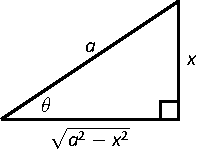
\includegraphics{figures/figtrigsub_intro1}
		\end{minipage}
		
	\item[(b)] \noindent
	\begin{minipage}[t]{.6\linewidth}
		For integrands containing $\sqrt{x^2+a^2}$:\\[5pt]
		Let $x=a\tan\theta$, \qquad $dx = a\sec^2\theta\ d\theta$\\[5pt]	
	Thus $\theta = \tan^{-1}(x/a)$, for $-\pi/2 < \theta < \pi/2$. \\[5pt]	
	On this interval, $\sec\theta> 0$, so\\[5pt]	
	$\sqrt{x^2+a^2} = a\sec\theta$
		\end{minipage}\qquad
	\begin{minipage}[t]{.4\linewidth}\vskip 0pt
		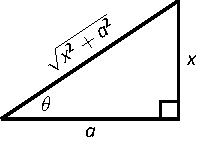
\includegraphics{figures/figtrigsub_intro3}
		\end{minipage}
		
	\item[(c)] \noindent
	\begin{minipage}[t]{.6\linewidth}
		For integrands containing $\sqrt{x^2-a^2}$:\\[5pt]
		Let $x=a\sec\theta$, \qquad $dx = a\sec\theta\tan\theta\ d\theta$\\[5pt]	
	Thus $\theta = \sec^{-1}(x/a)$. Note that $\sqrt{x^2-a^2}$ is defined for $x\geq a$ or $x\leq -a$.\\
	 If $x\geq a$, then $x/a\geq 1$ and $0\leq\theta<\pi/2$; if $x<-a$, then $x/a \leq -1$ and $\pi\leq\theta< \frac{3\pi}{2}$.\\[5pt]	
	On these intervals, $\tan\theta\geq 0$, so\\[5pt]	
	$\sqrt{x^2-a^2} = a\tan\theta$
		\end{minipage}\qquad
	\begin{minipage}[t]{.4\linewidth}\vskip 0pt
		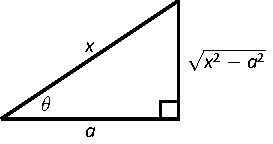
\includegraphics{figures/figtrigsub_intro2}
		\end{minipage}	
\end{enumerate}
}
\end{minipage}
\restoreboxwidth
\vskip \baselineskip

\example{ex_trigsub3}{Using Trigonometric Substitution}{
Evaluate $\ds \int \frac{1}{\sqrt{5+x^2}}\ dx.$}
{Using Key Idea \ref{idea:trigsub}(b), we recognize $a=\sqrt{5}$ and  set $x= \sqrt{5}\tan \theta$. This makes $dx = \sqrt{5}\sec^2\theta\ d\theta$. We will use the fact that $\sqrt{5+x^2} = \sqrt{5+5\tan^2\theta} = \sqrt{5\sec^2\theta} = \sqrt{5}\sec\theta.$ Substituting, we have:
\begin{align*}
\int \frac{1}{\sqrt{5+x^2}}\ dx &= \int \frac{1}{\sqrt{5+5\tan^2\theta}}\sqrt{5}\sec^2\theta\ d\theta \\
			&= \int \frac{\sqrt{5}\sec^2\theta}{\sqrt{5}\sec\theta} \ d\theta\\
			&= \int \sec\theta\ d\theta\\
			&= \ln\big|\sec\theta+\tan\theta\big|+C.
\end{align*}
While the integration steps are over, we are not yet done. The original problem was stated in terms of $x$, whereas our answer is given in terms of $\theta$. We must convert back to $x$.

The reference triangle given in Key Idea \ref{idea:trigsub}(b) helps. With $x=\sqrt{5}\tan\theta$, we have 
\[
\tan \theta = \frac x{\sqrt{5}}\quad \text{and}\quad \sec\theta = \frac{\sqrt{x^2+5}}{\sqrt{5}}.
\]
This gives
\begin{align*}
\int \frac{1}{\sqrt{5+x^2}}\ dx &= \ln\big|\sec\theta+\tan\theta\big|+C \\
     &= \ln\left|\frac{\sqrt{x^2+5}}{\sqrt{5}}+ \frac x{\sqrt{5}}\right|+C.
\end{align*}
We can leave this answer as is, or we can use a logarithmic identity to simplify it. Note:
\begin{align*}
\ln\left|\frac{\sqrt{x^2+5}}{\sqrt{5}}+ \frac x{\sqrt{5}}\right|+C &= \ln\left|\frac{1}{\sqrt{5}}\big(\sqrt{x^2+5}+ x\big)\right|+C \\
   &= \ln\left|\frac{1}{\sqrt{5}}\right| + \ln\big|\sqrt{x^2+5}+ x\big|+C\\
	&=	\ln\big|\sqrt{x^2+5}+ x\big|+C,
\end{align*}
where the $\ln\big(1/\sqrt{5}\big)$ term is absorbed into the constant $C$. (In Section \ref{sec:hyperbolic} we will learn another way of approaching this problem.)
}\\

\example{ex_trigsub2}{Using Trigonometric Substitution}{
Evaluate $\ds \int \sqrt{4x^2-1}\ dx$.}
{We start by rewriting the integrand so that it looks like $\sqrt{x^2-a^2}$ for some value of $a$:
\begin{align*}
\sqrt{4x^2-1} &= \sqrt{4\left(x^2-\frac14\right)}\\
		&= 2\sqrt{x^2-\left(\frac12\right)^2}.
\end{align*}
So we have $a=1/2$, and following Key Idea \ref{idea:trigsub}(c), we set $x= \frac12\sec\theta$, and hence $dx = \frac12\sec\theta\tan\theta\ d\theta$. %The Key Idea also shows that $\sqrt{x^2-1/2^2} = \frac12\tan\theta$. 
We now rewrite the integral with these substitutions:
\begin{align*}
\int \sqrt{4x^2-1}\ dx &= \int 2\sqrt{x^2-\left(\frac12\right)^2}\ dx\\
			&= \int 2\sqrt{\frac14\sec^2\theta - \frac14}\left(\frac12\sec\theta\tan\theta\right)\ d\theta\\
			&=\int \sqrt{\frac14(\sec^2\theta-1)}\Big(\sec\theta\tan\theta\Big)\ d\theta\\
			&=\int\sqrt{\frac14\tan^2\theta}\Big(\sec\theta\tan\theta\Big)\ d\theta\\
			&=\int \frac12\tan^2\theta\sec\theta\ d\theta\\
			&=\frac12\int \Big(\sec^2\theta-1\Big)\sec\theta\ d\theta\\
			&=\frac12\int \big(\sec^3\theta - \sec\theta\big)\ d\theta.
\end{align*}
We integrated $\sec^3\theta$ in Example \ref{ex_trigint6}, finding its antiderivatives to be
\[
\int \sec^3\theta\ d\theta = \frac12\Big(\sec \theta\tan \theta + \ln|\sec \theta+\tan \theta|\Big)+C.
\]
\enlargethispage{2\baselineskip}
Thus
\begin{align*}
\int \sqrt{4x^2-1}\ dx &=\frac12\int \big(\sec^3\theta - \sec\theta\big)\ d\theta\\
			&= \frac12\left(\frac12\Big(\sec \theta\tan \theta + \ln|\sec \theta+\tan \theta|\Big) -\ln|\sec \theta + \tan\theta|\right) + C\\
			%\end{align*}
			%\begin{align*}
			&= \frac14\left(\sec\theta\tan\theta -\ln|\sec\theta+\tan\theta|\right)+C.
\end{align*}
We are not yet done. Our original integral is given in terms of $x$, whereas our final answer, as given, is in terms of $\theta$. We need to rewrite our answer in terms of $x$. With $a=1/2$, and $x=\frac12\sec\theta$, the reference triangle in Key Idea \ref{idea:trigsub}(c) shows that 
\[
\tan \theta = \sqrt{x^2-1/4}\Big/(1/2) = 2\sqrt{x^2-1/4}\quad \text{and}\quad \sec\theta = 2x.
\]
Thus\small 
\begin{align*}
\frac14\Big(\sec\theta\tan\theta -\ln\big|\sec\theta+\tan\theta\big|\Big)+C &=
				\frac14\Big(2x\cdot 2\sqrt{x^2-1/4} - \ln\big|2x + 2\sqrt{x^2-1/4}\big|\Big)+C\\
				&= \frac14\Big(4x\sqrt{x^2-1/4} - \ln\big|2x + 2\sqrt{x^2-1/4}\big|\Big)+C.
\end{align*}
\normalsize 
The final answer is given in the last line above, repeated here:
\[
\int \sqrt{4x^2-1}\ dx = \frac14\Big(4x\sqrt{x^2-1/4} - \ln\big|2x + 2\sqrt{x^2-1/4}\big|\Big)+C.
\]
}\\

\example{ex_trigsub4}{Using Trigonometric Substitution}{
Evaluate $\ds \int \frac{\sqrt{4-x^2}}{x^2}\ dx$.}
{We use Key Idea \ref{idea:trigsub}(a) with $a=2$, $x=2\sin \theta$, $dx = 2\cos \theta$ and hence $\sqrt{4-x^2} = 2\cos\theta$. This gives
\begin{align*}
\int \frac{\sqrt{4-x^2}}{x^2}\ dx &= \int \frac{2\cos\theta}{4\sin^2\theta}(2\cos\theta)\ d\theta\\
		&= \int \cot^2\theta\ d\theta\\
		&=	\int (\csc^2\theta -1)\ d\theta\\
		&= -\cot\theta -\theta + C.
\end{align*}
We need to rewrite our answer in terms of $x$. Using the reference triangle found in Key Idea \ref{idea:trigsub}(a), we have $\cot\theta = \sqrt{4-x^2}/x$ and $\theta = \sin^{-1}(x/2)$. Thus
\[
\int \frac{\sqrt{4-x^2}}{x^2}\ dx = -\frac{\sqrt{4-x^2}}x-\sin^{-1}\left(\frac x2\right) + C.
\]
}\\

Trigonometric Substitution can be applied in many situations, even those not of the form $\sqrt{a^2-x^2}$, $\sqrt{x^2-a^2}$ or $\sqrt{x^2+a^2}$. In the following example, we apply it to an integral we already know how to handle.\\

\example{ex_trigsub5}{Using Trigonometric Substitution}{
Evaluate $\ds \int\frac1{x^2+1}\ dx$.}
{We know the answer already as $\tan^{-1}x+C$. We apply Trigonometric Substitution here to show that we get the same answer without inherently relying on knowledge of the derivative of the arctangent function.

Using Key Idea \ref{idea:trigsub}(b), let $x=\tan\theta$, $dx=\sec^2\theta\ d\theta$ and note that $x^2+1 = \tan^2\theta+1 = \sec^2\theta$. Thus
\begin{align*}
\int \frac1{x^2+1}\ dx &= \int \frac{1}{\sec^2\theta}\sec^2\theta\ d\theta \\
			&= \int 1\ d\theta\\
			&= \theta + C.
\end{align*}
Since $x=\tan \theta$, $\theta = \tan^{-1}x$, and we conclude that $\ds \int\frac1{x^2+1}\ dx = \tan^{-1}x+C.$
}\\

The next example is similar to the previous one in that it does not involve a square--root. It shows how several techniques and identities can be combined to obtain a solution.\\

\example{ex_trigsub7}{Using Trigonometric Substitution}{
Evaluate $\ds\int\frac1{(x^2+6x+10)^2}\ dx.$
}
{We start by completing the square, then make the substitution $u=x+3$, followed by the trigonometric substitution of $u=\tan\theta$:
\begin{align}
\int \frac1{(x^2+6x+10)^2}\ dx =\int \frac1{\big((x+3)^2+1\big)^2}\ dx&= \int \frac1{(u^2+1)^2}\ du. \notag
\intertext{Now make the substitution $u=\tan\theta$, $du=\sec^2\theta\ d\theta$:}
   &=	\int \frac1{(\tan^2\theta+1)^2}\sec^2\theta\ d\theta\notag\\
	&= \int\frac 1{(\sec^2\theta)^2}\sec^2\theta\ d\theta\notag\\
	&= \int \cos^2\theta\ d\theta.\notag
	\intertext{Applying a power reducing formula, we have}
	&= \int \left(\frac12 +\frac12\cos(2\theta)\right)\ d\theta \notag\\
	&= \frac12\theta + \frac14\sin(2\theta) + C.\label{eq:extrigsub7}
\end{align}
We need to return to the variable $x$. As $u=\tan\theta$, $\theta = \tan^{-1}u$. Using the identity $\sin(2\theta) = 2\sin\theta\cos\theta$ and using the reference triangle found in Key Idea \ref{idea:trigsub}(b), we have 
\[
\frac14\sin(2\theta) = \frac12\frac u{\sqrt{u^2+1}}\cdot\frac 1{\sqrt{u^2+1}} = \frac12\frac u{u^2+1}.
\]
Finally, we return to $x$ with the substitution $u=x+3$. We start with the expression in Equation \eqref{eq:extrigsub7}:
\begin{align*}
\frac12\theta + \frac14\sin(2\theta) + C &= \frac12\tan^{-1}u + \frac12\frac{u}{u^2+1}+C\\
				&= \frac12\tan^{-1}(x+3) + \frac{x+3}{2(x^2+6x+10)}+C.
\end{align*}
Stating our final result in one line,
\[
\int\frac1{(x^2+6x+10)^2}\ dx=\frac12\tan^{-1}(x+3) + \frac{x+3}{2(x^2+6x+10)}+C.
\]
}\\


Our last example returns us to definite integrals, as seen in our first example. Given a definite integral that can be evaluated using Trigonometric Substitution, we could first evaluate the corresponding indefinite integral (by changing from an integral in terms of $x$ to one in terms of $\theta$, then converting back to $x$) and then evaluate using the original bounds. It is much more straightforward, though, to change the bounds as we substitute.\\

\example{ex_trigsub6}{Definite integration and Trigonometric Substitution}{
Evaluate $\ds\int_0^5\frac{x^2}{\sqrt{x^2+25}}\ dx$.
}
{Using Key Idea \ref{idea:trigsub}(b), we set $x=5\tan\theta$, $dx = 5\sec^2\theta\ d\theta$, and note that $\sqrt{x^2+25} = 5\sec\theta$. As we substitute, we can also change the bounds of integration.

The lower bound of the original integral is $x=0$. As $x=5\tan\theta$, we solve for $\theta$ and find $\theta = \tan^{-1}(x/5)$. Thus the new lower bound is $\theta = \tan^{-1}(0) = 0$. The original upper bound is $x=5$, thus the new upper bound is $\theta = \tan^{-1}(5/5) = \pi/4$. 

Thus we have 
\begin{align*}
\int_0^5\frac{x^2}{\sqrt{x^2+25}}\ dx &= \int_0^{\pi/4} \frac{25\tan^2\theta}{5\sec\theta}5\sec^2\theta\ d\theta\\
		&= 25\int_0^{\pi/4} \tan^2\theta\sec\theta\ d\theta.
\end{align*}
We encountered this indefinite integral in Example \ref{ex_trigsub2} where we found 
\[
\int \tan^2\theta\sec\theta \ d\theta = \frac12\big(\sec\theta\tan\theta-\ln|\sec\theta+\tan\theta|\big).
\]
So
\begin{align*}
25\int_0^{\pi/4} \tan^2\theta\sec\theta\ d\theta &= \frac{25}2\big(\sec\theta\tan\theta-\ln|\sec\theta+\tan\theta|\big)\Bigg|_0^{\pi/4}\\
&= \frac{25}2\big(\sqrt2-\ln(\sqrt2+1)\big)\\
&\approx 6.661.
\end{align*}
\vskip-1.5\baselineskip
}\\

\enlargethispage{3\baselineskip}
The following equalities are very useful when evaluating integrals using Trigonometric Substitution. 

\keyidea{idea:useful_trigsub}{Useful Equalities with Trigonometric Substitution}
{\begin{enumerate}
	\item	$\sin(2\theta) = 2\sin\theta\cos\theta$
	\item	$\cos(2\theta) = \cos^2\theta - \sin^2\theta = 2\cos^2\theta-1 = 1-2\sin^2\theta$
	\item $\ds \int \sec^3\theta\ d\theta = \frac12\Big(\sec \theta\tan \theta + \ln\big|\sec \theta+\tan \theta\big|\Big)+C$
	\item	$\ds \int \cos^2\theta\ d\theta = \int \frac12\big(1+\cos(2\theta)\big)\ d\theta = \frac12\big(\theta+\sin\theta\cos\theta\big)+C.$
\end{enumerate}
}

%\subsection*{Hyperbolic substitution}
%For integrands containing terms of the form $\sqrt{x^2+a^2}$ or $\sqrt{x^2-a^2}$, it is also possible to make use of \sword{hyperbolic substitution} \index{substitution ! hyperbolic}. Recall from Section \ref{sec:hyperbolic} of the Math 1560 textbook that the hyperbolic functions are defined by
%\[
%\cosh(x) = \frac{e^x+e^{-x}}{2} \quad \text{ and } \quad \sinh(x) %= \frac{e^x-e^{-x}}{2},
%\]
%with $\tanh(x) = \dfrac{\sinh(x)}{\cosh(x)}$, and so on. Recall that the hyperbolic functions satisfy the identity
%\[
%\cosh^2(x)-\sinh^2(x)  = 1.
%\]
%If we're given $\sqrt{x^2+a^2}$, we can let $x=a\sinh(t)$, then
%\[
%x^2+a^2 = (a\sinh(t))^2+a^2 = a^2(\sinh^2(t)+1) = a^2\cosh^2(t),
%\]
%and $dx = a\cosh(t)\,dt$. Since $\cosh(t)>0$ for all real numbers $t$, we have $\sqrt{a^2+x^2}=\cosh(t)$.

%If we're given $\sqrt{x^2-a^2}$, we can let $x=a\cosh(t)$; then
%\[
%x^2-a^2 = (a\cosh(t))^2-a^2 = a^2(\cosh^2(t)-1) = a^2\sinh^2(t),
%\]
%and $dx = a\sinh(t)$. (One of the convenient aspects of working with hyperbolic functions is that there are no signs to worry about when taking derivatives.)
%Note that $\cosh(t)>0$ for all $t$, so the substitution $x=a\cosh(t)$ works in the case that $x\geq a>0$. In this case, $\sqrt{x^2-a^2} = a\sinh(t)$. For $x<-a<0$, technically we would need to let $x=-a\cosh(t)$. We illustrate this method with a couple of examples.\\

%\example{ex_hypsub1}{Using hyperbolic substitution}{
%Use hyperbolic substitution to evaluate the integral $\displaystyle \int\frac{3}{\sqrt{x^2+4}}\,dx$.
%}
%{
%Here we encounter the form $\sqrt{x^2+4} = \sqrt{x^2+2^2}$, so we use the substitution $x=2\sinh(t)$, or $t=\sinh^{-1}(x/2)$. This gives us
%\[
%\sqrt{x^2+4} = \sqrt{4\sinh^2(t)+4} = \sqrt{4\cosh^2(t)}=2\cosh(t),
%\]
%and $dx = 4\cosh(t)\,dt$. Substituting these into the integral, we have
%\begin{align*}
%\int\frac{3}{\sqrt{x^2+4}}\,dx &= \int \frac{3(2\cosh(t))}{2\cosh(t)}\,dt\\
%& = \int 3 \,dt = 3t+C\\
%& = 3\sinh^{-1}\left(\frac{x}{2}\right)+C.
%\end{align*}

%Of course, we could also evaluate the integral using the substitution $x=2\tan\theta$. In this case, the hyperbolic substitution turns out to be much simpler. Let's go through the details to confirm this. If $x=2\tan\theta$, then we have $dx = 2\sec^2\theta\,d\theta$, and
%\[
%\sqrt{x^2+4} = \sqrt{4\tan^2\theta+4} = \sqrt{4\sec^2\theta} = 2\sec\theta.
%\]
%In terms of $\theta$, our integral is
%\begin{align*}
%\int\frac{3}{\sqrt{x^2+4}}\,dx & = \int \frac{3(2\sec^2\theta)}{2\sec\theta}\,d\theta\\
% & = \int 3\sec\theta\,d\theta\\
% & = 3\ln\lvert \sec\theta +\tan\theta\rvert+C\\
% & = 3\ln\left( \frac{\sqrt{x^2+4}}{2} + \frac{x}{2}\right) +C.
%\end{align*}
%(Note that since $\sqrt{x^2+4}>x$ for all values of $x$, we can drop the absolute value in the argument of the logarithm.)

%The answer using the hyperbolic substitution certainly looks simpler, and it was easier to obtain, but are the two results equivalent? That is, is it true that
%\[
%\sinh^{-1}\left(\frac{x}{2}\right) = \ln\left(\frac{\sqrt{x^2+4}+x}{2}\right)?
%\]
%To check, let's take the hyperbolic sine of both sides. On the left, this yields $\frac{x}{2}$. On the right, we get
%\begin{align*}
%\sinh\left[\ln\left(\frac{\sqrt{x^2+4}+x}{2}\right)\right] & = \frac{1}{2}\left[e^{\ln\left(\frac{\sqrt{x^2+4}+x}{2}\right)}-e^{\ln\left(\frac{\sqrt{x^2+4}+x}{2}\right)}\right]\\
%& = \frac{1}{2}\left[\frac{\sqrt{x^2+4}+x}{2}-\frac{2}{\sqrt{x^2+4}+x}\right]\\
%& = \frac{1}{2}\left[\frac{(\sqrt{x^2+4}+x)^2-4}{2(\sqrt{x^2+4}+x)}\right]\\
%& = \frac{1}{4}\left[\frac{(x^2+4)+2x\sqrt{x^2+4}+x^2-4}{\sqrt{x^2+4}+x}\right]\\
%& = \frac{1}{4}\left[\frac{2x(\sqrt{x^2+4}+x)}{\sqrt{x^2+4}+x}\right]\\
%& = \frac{x}{2},
%\end{align*}
%so the results agree!
%}\\

%\example{ex_hypsub2}{Using hyperbolic substitution}{
%Evaluate the integral $\displaystyle \int\frac{x^2}{\sqrt{x^2-16}}\,dx$ using a hyperbolic substitution.
%}
%{Once again, we \textit{could} use the substitution $x=4\sec\theta$, but doing so leads us to a $\sec^3\theta$ integral, and those are never fun. (Feel free to try it this way) Instead, we decide to read (and follow) the instructions, and use a hyperbolic substitution.

%The form $\sqrt{x^2-16}$ tells us that we should try the substitution $x=4\cosh(t)$.  This gives us $dx = 4\sinh(t)$, and
% \[
% \sqrt{x^2-16} = \sqrt{16(\cosh^2(t)-1)} = \sqrt{16\sinh^2(t)} = 4\sinh(t).
% \]
% Thus,
% \[
% \int \frac{x^2}{\sqrt{x^2-16}}\,dx = \int \frac{16\cosh^2(t)}{4\sinh(t)}(4\sinh(t))\,dt = \int 16\cosh^2(t)\,dt.
% \]
% Now we have to know how to integrate $\cosh^2(t)$. If we recall how $\cosh(t)$ is defined, we have
% \[
% \cosh^2(t) = \left(\frac{e^t+e^{-t}}{2}\right)^2 = \frac{e^{2t}+e^{-2t}+2}{4}.
% \]
% So you could simply write $\cosh^2(t)$ in terms of exponentials as above, and integrate term-by-term. The other option is to notice that there's an identity sitting there: $\dfrac{e^{2t}+e^{-2t}}{4} = \frac{1}{2}\cosh(2t)$, so
% \[
% \int \cosh^2(t)\,dt = \int\left( \frac{1}{2}\cosh(2t)+\frac{1}{2}\right)\,dt = \frac{1}{4}\sinh(2t)+\frac{t}{2}+C.
% \]
% Finally, we have to substitute back in terms of $x$. Would it surprise you to learn that $\sinh(2t)=2\sinh(t)\cosh(t)$, just as it is with trig functions? Well, that turns out to be true (verify this!). Since $\sinh(t) = \frac{\sqrt{x^2-16}}{4}$ and $\cosh(t) = \frac{x}{4}$, we get
% \begin{align*}
% \int \frac{x^2}{\sqrt{x^2-16}}\,dx & =  16\int\cosh^2(t)\,dt\\
% & = \frac{1}{2}x\sqrt{x^2-16}+8\cosh^{-1}\left(\frac{x}{4}\right)+C.
% \end{align*}
% Again, if you chose the secant substitution route, you would have ended up with a very different-looking answer. This method gives
% \[
% \int\frac{x^2}{\sqrt{x^2-16}}\,dx = \frac{1}{2}x\sqrt{x^2-16}+8\ln\left(\frac{x+\sqrt{x^2-16}}{4}\right),
% \]
%and as with the last example, you might be wondering is whether the two answers are the same.  It's a good exercise to see if you can show that
% \[
% \ln\left(\frac{x+\sqrt{x^2-16}}{4}\right) = \cosh^{-1}(x/4).
% \]
%You can perform algebraic manipulations as before, or check that the derivatives of both sides are the same (it's enough for the answers to agree up to a constant).
%}\\

The next section introduces Partial Fraction Decomposition, which is an algebraic technique that turns ``complicated'' fractions into sums of ``simpler'' fractions, making integration easier.

\printexercises{exercises/06_08_exercises}




\section{Partial Fraction Decomposition}\label{sec:partial_fraction}

In this section we investigate the antiderivatives of rational functions. Recall that rational functions are functions of the form $f(x)= \frac{p(x)}{q(x)}$, where $p(x)$ and $q(x)$ are polynomials and $q(x)\neq 0$. Such functions arise in many contexts, one of which is the solving of certain fundamental differential equations.

We begin with an example that demonstrates the motivation behind this section. Consider the integral $\ds\int \frac{1}{x^2-1}\ dx$. We do not have a simple formula for this (if the denominator were $x^2+1$, we would recognize the antiderivative as being the arctangent function). It can be solved using Trigonometric Substitution, but note how the integral is easy to evaluate once we realize:

%This integral is not difficult to evaluate once one realizes the following fact: 
\[
\frac{1}{x^2-1} = \frac{1/2}{x-1} - \frac{1/2}{x+1}.
\]
Thus 
\begin{align*}
\int\frac{1}{x^2-1}\ dx &= \int\frac{1/2}{x-1}\ dx - \int\frac{1/2}{x+1}\ dx \\
			&= \frac12\ln|x-1| - \frac12\ln|x+1| + C.
\end{align*}

This section teaches how to \textit{decompose} 
\[
\frac{1}{x^2-1}\quad  \text{into}\quad  \frac{1/2}{x-1}-\frac{1/2}{x+1}.
\]

We start with a rational function $f(x)=\dfrac{p(x)}{q(x)}$, where $p$ and $q$ do not have any common factors and the degree of $p$ is less than the degree of $q$. Note that in the case of a function $f(x) = \dfrac{p(x)}{q(x)}$ where the degree of $p$ is greater than or equal to that of $q$, we can perform polynomial long division to rewrite $f(x)$ in the form
\[
f(x) = Q(x)+\frac{R(x)}{q(x)},
\]
where $Q(x)$ is the quotient polynomial, and $R(x)$, the remainder, always has degree less than that of $q$. 

It can be shown that any polynomial, and hence $q$, can be factored into a product of linear and irreducible quadratic terms. The following Key Idea states how to decompose a rational function into a sum of rational functions whose denominators are all of lower degree than $q$.
%\clearpage

\keyidea{idea:partial_fraction}{Partial Fraction Decomposition}
{Let $\ds \frac{p(x)}{q(x)}$ be a rational function, where the degree of $p$ is less than the degree of $q$.\index{integration!partial fraction decomp.}
\begin{enumerate}
	\item	\textbf{Linear Terms:} Let $(x-a)$ divide $q(x)$, where $(x-a)^n$ is the highest power of $(x-a)$ that divides $q(x)$. Then the decomposition of $\frac{p(x)}{q(x)}$ will contain the sum
	\[
	\frac{A_1}{(x-a)} + \frac{A_2}{(x-a)^2} + \cdots +\frac{A_n}{(x-a)^n}.
	\]
	\item		\textbf{Quadratic Terms:} Let $x^2+bx+c$ divide $q(x)$, where $(x^2+bx+c)^n$ is the highest power of $x^2+bx+c$ that divides $q(x)$. Then the decomposition of $\frac{p(x)}{q(x)}$ will contain the sum 
	\[
	\frac{B_1x+C_1}{x^2+bx+c}+\frac{B_2x+C_2}{(x^2+bx+c)^2}+\cdots+\frac{B_nx+C_n}{(x^2+bx+c)^n}.
	\]
	\end{enumerate}
	To find the coefficients $A_i$, $B_i$ and $C_i$:
	\begin{enumerate}
	\item	Multiply all fractions by $q(x)$, clearing the denominators. Collect like terms.
	\item		Equate the resulting coefficients of the powers of $x$ and solve the resulting system of linear equations.
	\end{enumerate}
}

The following examples will demonstrate how to put this Key Idea into practice. Example \ref{ex_pf1} stresses the decomposition aspect of the Key Idea.\\

\example{ex_pf1}{Decomposing into partial fractions}{
Decompose $\ds f(x)=\frac{1}{(x+5)(x-2)^3(x^2+x+2)(x^2+x+7)^2}$ without solving for the resulting coefficients.}
{The denominator is already factored, as both $x^2+x+2$ and $x^2+x+7$ cannot be factored further. We need to decompose $f(x)$ properly. Since $(x+5)$ is a linear term that divides the denominator, there will be a 
\[
\frac{A}{x+5}
\]
term in the decomposition.

As $(x-2)^3$ divides the denominator, we will have the following terms in the decomposition:
\[
\frac{B}{x-2},\quad \frac{C}{(x-2)^2}\quad \text{and}\quad \frac{D}{(x-2)^3}.
\]

The $x^2+x+2$ term in the denominator results in a $\ds\frac{Ex+F}{x^2+x+2}$ term.

Finally, the $(x^2+x+7)^2$ term results in the terms 
\[
\frac{Gx+H}{x^2+x+7}\quad \text{and}\quad \frac{Ix+J}{(x^2+x+7)^2}.
\]
All together, we have 
\begin{align*}
\frac{1}{(x+5)(x-2)^3(x^2+x+2)(x^2+x+7)^2} &= \frac{A}{x+5} + \frac{B}{x-2}+ \frac{C}{(x-2)^2}+\frac{D}{(x-2)^3}+ \\
		& \frac{Ex+F}{x^2+x+2}+\frac{Gx+H}{x^2+x+7}+\frac{Ix+J}{(x^2+x+7)^2}
\end{align*}
Solving for the coefficients $A$, $B \ldots J$ would be a bit tedious but not ``hard.''
}\\

\example{ex_pf2}{Decomposing into partial fractions}{
Perform the partial fraction decomposition of $\ds \frac{1}{x^2-1}$.}
{The denominator factors into two linear terms: $x^2-1 = (x-1)(x+1)$. Thus 
\[
\frac{1}{x^2-1} = \frac{A}{x-1} + \frac{B}{x+1}.
\]
To solve for $A$ and $B$, first multiply through by $x^2-1 = (x-1)(x+1)$:
\begin{align*}
1 &= \frac{A(x-1)(x+1)}{x-1}+\frac{B(x-1)(x+1)}{x+1} \\
	&= A(x+1) + B(x-1)\\
	&= Ax+A + Bx-B \\
	\intertext{Now collect like terms.}
	&= (A+B)x + (A-B).
\end{align*}
The next step is key. Note the equality we have:
\[
1 = (A+B)x+(A-B).
\]
For clarity's sake, rewrite the left hand side as
\[
0x+1 = (A+B)x+(A-B).
\]
On the left, the coefficient of the $x$ term is 0; on the right, it is $(A+B)$. Since both sides are equal, we must have that $0=A+B$. 

Likewise, on the left, we have a constant term of 1; on the right, the constant term is $(A-B)$. Therefore we have $1=A-B$.

We have two linear equations with two unknowns. This one is easy to solve by hand, leading to 
\[
\begin{array}{c} A+B = 0 \\ A-B = 1 \end{array} \Rightarrow \begin{array}{c} A=1/2 \\ B = -1/2\end{array}.
\]
Thus 
\[
\frac{1}{x^2-1} = \frac{1/2}{x-1}-\frac{1/2}{x+1}.
\]
\vskip-\baselineskip
}\\

\example{ex_pf3}{Integrating using partial fractions}{
Use partial fraction decomposition to integrate $\ds\int\frac{1}{(x-1)(x+2)^2}\ dx.$}
{We decompose the integrand as follows, as described by Key Idea \ref{idea:partial_fraction}:
\[
\frac{1}{(x-1)(x+2)^2} = \frac{A}{x-1} + \frac{B}{x+2} + \frac{C}{(x+2)^2}.
\]
To solve for $A$, $B$ and $C$, we multiply both sides by $(x-1)(x+2)^2$ and collect like terms:
\begin{align}
1 &= A(x+2)^2 + B(x-1)(x+2) + C(x-1)\label{eq:pf3}\\
	&= Ax^2+4Ax+4A + Bx^2 + Bx-2B + Cx-C \notag \\
	&= (A+B)x^2 + (4A+B+C)x + (4A-2B-C)\notag
\end{align}
\mnote{.7}{\textbf{Note:} Equation \ref{eq:pf3} offers a direct route to finding the values of $A$, $B$ and $C$. Since the equation holds for all values of $x$, it holds in particular when $x=1$. However, when $x=1$, the right hand side simplifies to $A(1+2)^2 = 9A$. Since the left hand side is still 1, we have $1 = 9A$. Hence $A = 1/9$.

Likewise, the equality holds when $x=-2$; this leads to the equation $1=-3C$. Thus $C = -1/3$.

Knowing $A$ and $C$, we can find the value of $B$ by choosing yet another value of $x$, such as $x=0$, and solving for $B$.}
We have 
\[
0x^2+0x+ 1 = (A+B)x^2 + (4A+B+C)x + (4A-2B-C)
\]
leading to the equations 
\[
A+B = 0, \quad 4A+B+C = 0 \quad \text{and} \quad 4A-2B-C = 1.
\]
These three equations of three unknowns lead to a unique solution:
\[
A = 1/9,\quad B = -1/9 \quad \text{and} \quad C = -1/3.
\]
Thus 
\[
\int\frac{1}{(x-1)(x+2)^2}\ dx = \int \frac{1/9}{x-1}\ dx + \int \frac{-1/9}{x+2}\ dx + \int \frac{-1/3}{(x+2)^2}\ dx.
\]

Each can be integrated with a simple substitution with $u=x-1$ or $u=x+2$ (or by directly applying Key Idea \ref{idea:linearsub} as the denominators are linear functions). The end result is
\[
\int\frac{1}{(x-1)(x+2)^2}\ dx = \frac19\ln|x-1| -\frac19\ln|x+2| +\frac1{3(x+2)}+C.
\]
\vskip-\baselineskip}\\

%\enlargethispage{\baselineskip}
\example{ex_pf4}{Integrating using partial fractions}{
Use partial fraction decomposition to integrate $\ds \int \frac{x^3}{(x-5)(x+3)}\ dx$.}
{Key Idea \ref{idea:partial_fraction} presumes that the degree of the numerator is less than the degree of the denominator. Since this is not the case here, we begin by using polynomial division to reduce the degree of the numerator. We omit the steps, but encourage the reader to verify that 
\[
\frac{x^3}{(x-5)(x+3)} = x+2+\frac{19x+30}{(x-5)(x+3)}.
\]
Using Key Idea \ref{idea:partial_fraction}, we can rewrite the new rational function as:
\[
\frac{19x+30}{(x-5)(x+3)} = \frac{A}{x-5} + \frac{B}{x+3}
\]
for appropriate values of $A$ and $B$. Clearing denominators, we have 

\mnote{.4}{\textbf{Note:} The values of $A$ and $B$ can be quickly found using the technique described in the margin of Example \ref{ex_pf3}.}

\begin{align*}
19x+30 &= A(x+3) + B(x-5)\\
			&= (A+B)x + (3A-5B).
\intertext{This implies that:}
19&= A+B \\
30&= 3A-5B.\\
\intertext{Solving this system of linear equations gives}
125/8 &=A\\
27/8 &=B.
\end{align*}

We can now integrate.
\begin{align*}
\int \frac{x^3}{(x-5)(x+3)}\ dx &= \int\left(x+2+\frac{125/8}{x-5}+\frac{27/8}{x+3}\right)\ dx \\
					&= \frac{x^2}2 + 2x + \frac{125}{8}\ln|x-5| + \frac{27}8\ln|x+3| + C.
\end{align*}
\vskip-\baselineskip
}\\
%\clearpage

\example{ex_pf5}{Integrating using partial fractions}{
Use partial fraction decomposition to evaluate $\ds \int\frac{7x^2+31x+54}{(x+1)(x^2+6x+11)}\ dx.$}
{The degree of the numerator is less than the degree of the denominator so we begin by applying Key Idea \ref{idea:partial_fraction}. We have:
\begin{align*}
\frac{7x^2+31x+54}{(x+1)(x^2+6x+11)} &= \frac{A}{x+1} + \frac{Bx+C}{x^2+6x+11}. \\
\intertext{Now clear the denominators.}
7x^2+31x+54 &= A(x^2+6x+11) + (Bx+C)(x+1)\\
					&= (A+B)x^2 + (6A+B+C)x + (11A+C).\\
\intertext{This implies that:}
				7&=A+B\\
				31 &= 6A+B+C\\
				54 &= 11A+C.
\end{align*}
Solving this system of linear equations gives the nice result of $A=5$, $B = 2$ and $C=-1$. Thus
\[
\int\frac{7x^2+31x+54}{(x+1)(x^2+6x+11)}\ dx = \int\left(\frac{5}{x+1} + \frac{2x-1}{x^2+6x+11}\right)\ dx.
\]

The first term of this new integrand is easy to evaluate; it leads to a $5\ln|x+1|$ term. The second term is not hard, but takes several steps and uses substitution techniques.

The integrand $\ds \frac{2x-1}{x^2+6x+11}$ has a quadratic in the denominator and a linear term in the numerator. This leads us to try substitution. Let $u = x^2+6x+11$, so $du = (2x+6)\ dx$. The numerator is $2x-1$, not $2x+6$, but we can get a $2x+6$ term in the numerator by adding 0 in the form of ``$7-7$.''
\begin{align*}
\frac{2x-1}{x^2+6x+11} &= \frac{2x-1+7-7}{x^2+6x+11} \\
					&= \frac{2x+6}{x^2+6x+11} - \frac{7}{x^2+6x+11}.
\end{align*}
We can now integrate the first term with substitution, leading to a $\ln|x^2+6x+11|$ term. The final term can be integrated using arctangent. First, complete the square in the denominator:
\[
\frac{7}{x^2+6x+11} = \frac{7}{(x+3)^2+2}.
\]
An antiderivative of the latter term can be found using Theorem \ref{thm:int_inverse_trig} and substitution:
\[
\int \frac{7}{x^2+6x+11}\ dx = \frac{7}{\sqrt{2}}\tan^{-1}\left(\frac{x+3}{\sqrt{2}}\right)+C.
\]

Let's start at the beginning and put all of the steps together.
\small\begin{align*}
\int\frac{7x^2+31x+54}{(x+1)(x^2+6x+11)}\ dx &= \int\left(\frac{5}{x+1} + \frac{2x-1}{x^2+6x+11}\right)\ dx \\
			&= \int\frac{5}{x+1}\ dx  + \int\frac{2x+6}{x^2+6x+11}\ dx -\int\frac{7}{x^2+6x+11}\ dx \\
			&= 5\ln|x+1|+ \ln|x^2+6x+11| -\frac{7}{\sqrt{2}}\tan^{-1}\left(\frac{x+3}{\sqrt{2}}\right)+C.
\end{align*}\normalsize
As with many other problems in calculus, it is important to remember that one is not expected to ``see'' the final answer immediately after seeing the problem. Rather, given the initial problem, we break it down into smaller problems that are easier to solve. The final answer is a combination of the answers of the smaller problems.
}\\

Partial Fraction Decomposition is an important tool when dealing with rational functions. Note that at its heart, it is a technique of algebra, not calculus, as we are rewriting a fraction in a new form. Regardless, it is very useful in the realm of calculus as it lets us evaluate a certain set of ``complicated'' integrals.

The next section introduces new functions, called the Hyperbolic Functions. They will allow us to make substitutions similar to those found when studying Trigonometric Substitution, allowing us to approach even more integration problems. 


\printexercises{exercises/06_04_exercises}

\section{Hyperbolic Functions}\label{sec:hyperbolic}

The \textbf{hyperbolic functions} are a set of functions that have many applications to mathematics, physics, and engineering. Among many other applications, they are used to describe the formation of satellite rings around planets, to describe the shape of a rope hanging from two points, and have application to the theory of special relativity. This section defines the hyperbolic functions and describes many of their properties, especially their usefulness to calculus.

These functions are sometimes referred to as the ``hyperbolic trigonometric functions'' as there are many, many connections between them and the standard trigonometric functions. Figure \ref{fig:hfcircle} demonstrates one such connection. Just as cosine and sine are used to define points on the circle defined by $x^2+y^2=1$, the functions \textbf{hyperbolic cosine} and \textbf{hyperbolic sine} are used to define points on the hyperbola $x^2-y^2=1$.

\mtable{.7}{Using trigonometric functions to define points on a circle and hyperbolic functions to define points on a hyperbola. The area of the shaded regions are included in them.}{fig:hfcircle}{\myincludegraphics{figures/fighf_circlearea}\vskip10pt\myincludegraphics{figures/fighf_hyperbolaarea}}

We begin with their definition.

\definition{def:hyperbolic_functions}{Hyperbolic Functions}
{\noindent%
\begin{minipage}{.5\specialboxlength}
\begin{enumerate}
\item		$\ds \cosh x = \frac{e^x+e^{-x}}2$\index{hyperbolic function!definition}
\item		$\ds \sinh x = \frac{e^x-e^{-x}}2$
\item		$\ds \tanh x = \frac{\sinh x}{\cosh x}$
\end{enumerate}
\end{minipage}
\begin{minipage}{.5\specialboxlength}
\begin{enumerate}\addtocounter{enumi}{3}
\item		$\ds \sech x = \frac{1}{\cosh x}$
\item		$\ds \csch x = \frac{1}{\sinh x}$
\item		$\ds \coth x = \frac{\cosh x}{\sinh x}$
\end{enumerate}
\end{minipage}
}\\

These hyperbolic functions are graphed in Figure \ref{fig:hyperbolic}. In the graphs of $\cosh x$ and $\sinh x$, graphs of $e^x/2$ and $e^{-x}/2$ are included with dashed lines. As $x$ gets ``large,'' $\cosh x$ and $\sinh x$ each act like $e^x/2$; when $x$ is a large negative number, $\cosh x$ acts like $e^{-x}/2$ whereas $\sinh x$ acts like $-e^{-x}/2$.

Notice the domains of $\tanh x$ and $\sech x$ are $(-\infty,\infty)$, whereas both $\coth x$ and $\csch x$ have vertical asymptotes at $x=0$. Also note the ranges of these functions, especially $\tanh x$: as $x\to\infty$, both $\sinh x$ and $\cosh x$ approach $e^{x}/2$, hence $\tanh x$ approaches $1$.

%It is no coincidence that these functions share a name similar to the trigonometric functions. 
The following example explores some of the properties of these functions that bear remarkable resemblance to the properties of their trigonometric counterparts.\\

\mnote{.4}{\textbf{Pronunciation Note:} \par 
``cosh'' rhymes with ``gosh,'' \par ``sinh'' rhymes with ``pinch,'' and \par ``tanh'' rhymes with ``ranch.''}

\clearpage
\begin{center}
\begin{tabular}{ccc}
\myincludegraphics{figures/fighf_cosh} &\ \hskip 25pt\ & \myincludegraphics{figures/fighf_sinh} \\[20pt]
\myincludegraphics{figures/fighf_tanh_coth}& &\myincludegraphics{figures/fighf_sech_csch}
\end{tabular}
\captionsetup{type=figure}
\caption{Graphs of the hyperbolic functions.}\label{fig:hyperbolic}
\end{center}
\vskip\baselineskip

\example{ex_hf1}{Exploring properties of hyperbolic functions}{
\noindent Use Definition \ref{def:hyperbolic_functions} to rewrite the following expressions.

\noindent\begin{minipage}{.5\linewidth}
\begin{enumerate}
\item		$\cosh^2 x-\sinh^2x$
\item		$\tanh^2 x+\sech^2 x$
\item		$2\cosh x\sinh x$
\end{enumerate}
\end{minipage}
\begin{minipage}{.5\linewidth}
\begin{enumerate}\addtocounter{enumi}{3}
\item		$\frac{d}{dx}\big(\cosh x\big)$
\item		$\frac{d}{dx}\big(\sinh x\big)$
\item		$\frac{d}{dx}\big(\tanh x\big)$
\end{enumerate}
\end{minipage}
}
{\begin{enumerate}
\item		%\vskip-\baselineskip%
\hfill$\begin{aligned}[t]
 \cosh^2x-\sinh^2x &= \left(\frac{e^x+e^{-x}}2\right)^2 -\left(\frac{e^x-e^{-x}}2\right)^2\\
 						&= \frac{e^{2x}+2e^xe^{-x} + e^{-2x}}4 - \frac{e^{2x}-2e^xe^{-x} + e^{-2x}}4\\
 						&= \frac44=1.
\end{aligned}$\hfill

So $\cosh^2 x-\sinh^2x=1$.

\item		\hfill$\begin{aligned}[t]
\tanh^2 x+\sech^2 x &=\frac{\sinh^2x}{\cosh^2 x} + \frac{1}{\cosh^2 x} \\
					&= \frac{\sinh^2x+1}{\cosh^2 x}\qquad \text{\small Now use identity from \#1.}\\
					&= \frac{\cosh^2 x}{\cosh^2 x} = 1.
\end{aligned}$\hfill

%%% Figure of the hyperbolic functions
%\mtable{.55}{Graphs of the hyperbolic functions.}{fig:hyperbolic}{\myincludegraphics{figures/fighf_cosh}\vskip 10pt \myincludegraphics{figures/fighf_sinh} \vskip 10pt\myincludegraphics{figures/fighf_tanh_coth}\vskip 10pt\myincludegraphics{figures/fighf_sech_csch}}
%%%


So $\tanh^2 x+\sech^2 x=1$.



\item \hfill$\begin{aligned}[t]
	2\cosh x\sinh x &= 2\left(\frac{e^x+e^{-x}}2\right)\left(\frac{e^x-e^{-x}}2\right) \\
					&= 2 \cdot\frac{e^{2x} - e^{-2x}}4\\
					&= \frac{e^{2x} - e^{-2x}}2 = \sinh (2x).\\
			\end{aligned}$ \hfill
			
Thus $2\cosh x\sinh x = \sinh (2x)$.

\item  \hfill$\begin{aligned}[t]
	\frac{d}{dx}\big(\cosh x\big) &= \frac{d}{dx}\left(\frac{e^x+e^{-x}}2\right) \\
					&= \frac{e^x-e^{-x}}2\\
					&= \sinh x.
	\end{aligned}\hfill$

So $\frac{d}{dx}\big(\cosh x\big) = \sinh x.$
	
\item  \hfill$\begin{aligned}[t]
	\frac{d}{dx}\big(\sinh x\big) &= \frac{d}{dx}\left(\frac{e^x-e^{-x}}2\right) \\
					&= \frac{e^x+e^{-x}}2\\
					&= \cosh x.
	\end{aligned}\hfill$

So $\frac{d}{dx}\big(\sinh x\big) = \cosh x.$
	
\item  \hfill$\begin{aligned}[t]
	\frac{d}{dx}\big(\tanh x\big) &= \frac{d}{dx}\left(\frac{\sinh x}{\cosh x}\right) \\
					&= \frac{\cosh x \cosh x - \sinh x \sinh x}{\cosh^2 x}\\
					&= \frac{1}{\cosh^2 x}\\
					&= \sech^2 x.
	\end{aligned}\hfill$

So $\frac{d}{dx}\big(\tanh x\big) = \sech^2 x.$	
\end{enumerate}
\vskip-\baselineskip
}\\

The following Key Idea summarizes many of the important identities relating to hyperbolic functions. Each can be verified by referring back to Definition \ref{def:hyperbolic_functions}.

\setboxwidth{160pt}
%\noindent\ifthenelse{\isodd{\thepage}}{}{\hskip -160pt}%
\noindent\begin{minipage}{\specialboxlength}
\keyidea{idea:hyperbolic_identities}{Useful Hyperbolic Function Properties}
{\begin{minipage}[t]{.33\specialboxlength}
\textbf{Basic Identities}\par
\begin{enumerate}
\item $\cosh^2x-\sinh^2x=1$%
\index{hyperbolic function!identities}\index{hyperbolic function!derivatives}\index{hyperbolic function!integrals}\index{derivative!hyperbolic funct.}\index{integration!hyperbolic funct.}%
\item	$\tanh^2x+\sech^2x=1$
\item	$\coth^2x-\csch^2x = 1$
\item	$\cosh 2x=\cosh^2x+\sinh^2x$
\item	$\sinh 2x = 2\sinh x\cosh x$
\item	$\ds\cosh^2x = \frac{\cosh 2x+1}{2}$
\item $\ds \sinh^2x=\frac{\cosh 2x-1}{2}$
\end{enumerate}
\end{minipage}
\begin{minipage}[t]{.33\specialboxlength}
\textbf{Derivatives}
\begin{enumerate}
\item $\frac{d}{dx}\big(\cosh x\big) = \sinh x$
\item $\frac{d}{dx}\big(\sinh x\big) = \cosh x$
\item $\frac{d}{dx}\big(\tanh x\big) = \sech^2 x$
\item $\frac{d}{dx}\big(\sech x\big) = -\sech x\tanh x$
\item $\frac{d}{dx}\big(\csch x\big) = -\csch x\coth x$
\item $\frac{d}{dx}\big(\coth x\big) = -\csch^2x$
\end{enumerate}
\end{minipage}
\begin{minipage}[t]{.33\specialboxlength}
\textbf{Integrals}
\begin{enumerate}
\item $\ds\int \cosh x\ dx = \sinh x+C$
\item $\ds\int \sinh x\ dx = \cosh x+C$
\item $\ds\int \tanh x\ dx = \ln(\cosh x) +C$
\item $\ds\int \coth x\ dx = \ln|\sinh x\,|+C$
\end{enumerate}
\end{minipage}
}
\end{minipage}
\restoreboxwidth
\\

We practice using Key Idea \ref{idea:hyperbolic_identities}.\\

\example{ex_hf2}{Derivatives and integrals of hyperbolic functions}{
Evaluate the following derivatives and integrals.

\begin{minipage}[t]{.5\linewidth}
\begin{enumerate}
\item		$\ds\frac{d}{dx}\big(\cosh 2x\big)$
\item		$\ds\int \sech^2(7t-3)\ dt$
\end{enumerate}
\end{minipage}
\begin{minipage}[t]{.5\linewidth}
\begin{enumerate}\addtocounter{enumi}{2}
\item		$\ds \int_0^{\ln 2} \cosh x\ dx$
\end{enumerate}
\end{minipage}
}
{\begin{enumerate}
\item		Using the Chain Rule directly, we have $\frac{d}{dx} \big(\cosh 2x\big) = 2\sinh 2x$.

Just to demonstrate that it works, let's also use the Basic Identity found in Key Idea \ref{idea:hyperbolic_identities}: $\cosh 2x = \cosh^2x+\sinh^2x$.
\begin{align*}\frac{d}{dx}\big(\cosh 2x\big) = \frac{d}{dx}\big(\cosh^2x+\sinh^2x\big) &= 2\cosh x\sinh x+ 2\sinh x\cosh x\\ &= 4\cosh x\sinh x.
\end{align*}
Using another Basic Identity, we can see that $4\cosh x\sinh x = 2\sinh 2x$. We get the same answer either way.

\item	  We employ substitution, with $u = 7t-3$ and $du = 7dt$. Applying Key Ideas \ref{idea:linearsub}  and \ref{idea:hyperbolic_identities} we have:
\[
 \int \sech^2 (7t-3)\ dt = \frac17\tanh (7t-3) + C.
\]

\item		\[
			\int_0^{\ln 2} \cosh x\ dx = \sinh x\Big|_0^{\ln 2} = \sinh (\ln 2) - \sinh 0 = \sinh(\ln 2).
			\]

We can simplify this last expression as $\sinh x$ is based on exponentials:
\[
\sinh(\ln 2) = \frac{e^{\ln 2}-e^{-\ln 2}}2 = \frac{2-1/2}{2} = \frac34.
\]
\end{enumerate}
\vskip-1.5\baselineskip
}\pagebreak

\noindent\textbf{\large Inverse Hyperbolic Functions}\\

Just as the inverse trigonometric functions are useful in certain integration problems, the inverse hyperbolic functions are useful with others. Figure \ref{fig:hfinverse2} shows the restrictions on the domains to make each function one-to-one and the resulting domains and ranges of their inverse functions. Their graphs are shown in Figure \ref{fig:hfinverse1}.\index{hyperbolic function!inverse}

Because the hyperbolic functions are defined in terms of exponential functions, their inverses can be expressed in terms of logarithms as shown in Key Idea \ref{idea:hyperbolic_log}. It is often more convenient to refer to $\sinh^{-1}x$ than to $\ln\big(x+\sqrt{x^2+1}\big)$, especially when one is working on theory and does not need to compute actual values. On the other hand, when computations are needed, technology is often helpful but many hand-held calculators lack a \textit{convenient} $\sinh^{-1}x$ button. (Often it can be accessed under a menu system, but not conveniently.) In such a situation, the logarithmic representation is useful. The reader is not encouraged to memorize these, but rather know they exist and know how to use them when needed.
%\clearpage


%\mtable{.7}{Graphs of $\cosh x$, $\sinh x$ and their inverses.}{fig:hfinverse3}{\myincludegraphics{figures/fighfarccosh} \vskip 10pt\myincludegraphics{figures/fighfarcsinh}}
%
%\mtable{.3}{Graphs of $\tanh^{-1} x$, $\coth^{-1} x$, $\sech^{-1} x$ and $\csch^{-1} x$.}{fig:hfinverse4}{\myincludegraphics{figures/fighfarctanharccoth} \vskip 10pt\myincludegraphics{figures/fighfarcsecharccsch}}

%\clearpage

\hskip-.5\textwidth
\noindent\begin{minipage}{1.3\textwidth}
%\centering
\small
\begin{tabular}{ccc}
Function & Domain & Range\\ \hline
$\cosh x$ & $[0,\infty)$ & $[1,\infty)$\\
$\sinh x$ & $(-\infty,\infty)$ & $(-\infty,\infty)$\\
$\tanh x$ & $(-\infty,\infty)$ & $(-1,1)$\\
$\sech x$ & $[0,\infty)$ & $(0,1]$ \\
$\csch x$ & $(-\infty,0) \cup (0,\infty)$ & $(-\infty,0) \cup (0,\infty)$\\
$\coth x$ & $(-\infty,0) \cup (0,\infty)$ & $(-\infty,-1) \cup (1,\infty)$
\end{tabular}
\hskip 40pt
%\end{minipage}\hskip 40pt
%\begin{minipage}{.7\textwidth}
%\centering\small
\begin{tabular}{ccc}
Function & Domain & Range\\ \hline
\rule{0pt}{10pt}$\cosh^{-1} x$ & $[1,\infty)$ & $[0,\infty)$ \\
$\sinh^{-1} x$ & $(-\infty,\infty)$ & $(-\infty,\infty)$\\
$\tanh^{-1} x$ & $(-1,1)$ & $(-\infty,\infty)$\\
$\sech^{-1} x$ & $(0,1]$ & $[0,\infty)$ \\
$\csch^{-1} x$ & $(-\infty,0) \cup (0,\infty)$ & $(-\infty,0) \cup (0,\infty)$\\
$\coth^{-1} x$ & $(-\infty,-1) \cup (1,\infty)$ & $(-\infty,0) \cup (0,\infty)$
\end{tabular}
%\captionsetup{type=figure}%
%\caption{Restricted domains and ranges of the hyperbolic functions.}\label{fig:hfinverse1}
\captionsetup{type=figure}%
\caption{Domains and ranges of the hyperbolic and inverse hyperbolic functions.}\label{fig:hfinverse2}
\end{minipage}
%\enlargethispage{3\baselineskip}

%\hskip-100pt
\noindent \begin{minipage}{1.3\textwidth}
\begin{tabular}{ccc}
\myincludegraphics[scale=0.95]{figures/fighfarccosh} & \ \hskip 15pt\ &\myincludegraphics[scale=0.95]{figures/fighfarcsinh}\\[15pt]
\myincludegraphics[scale=0.95]{figures/fighfarctanharccoth} & &\myincludegraphics[scale=0.95]{figures/fighfarcsecharccsch}
\end{tabular}
\captionsetup{type=figure}%
\caption{Graphs of the hyperbolic functions and their inverses.}\label{fig:hfinverse1}
\end{minipage}

\setboxwidth{120pt}
%\noindent\hskip-120pt
\noindent\begin{minipage}{\specialboxlength}
\keyidea{idea:hyperbolic_log}{Logarithmic definitions of Inverse Hyperbolic Functions}
{\noindent%
\begin{minipage}[t]{.5\specialboxlength}
\begin{enumerate}
\item $\ds\cosh^{-1}x=\ln\big(x+\sqrt{x^2-1}\big);\ x\geq1$\index{hyperbolic function!inverse!logarithmic def.}\rule[-10pt]{0pt}{20pt}
\item $\ds\tanh^{-1}x = \frac12\ln\left(\frac{1+x}{1-x}\right);\ |x|<1$\rule[-10pt]{0pt}{20pt}
\item $\ds \sech^{-1}x = \ln\left(\frac{1+\sqrt{1-x^2}}x\right);\ 0<x\leq1$\rule[-10pt]{0pt}{20pt}
\end{enumerate}
\end{minipage}
\begin{minipage}[t]{.5\specialboxlength}
\begin{enumerate}\addtocounter{enumi}{3}
\item $\ds\sinh^{-1}x = \ln\big(x+\sqrt{x^2+1}\big)$\rule[-10pt]{0pt}{20pt}
\item	 $\ds\coth^{-1}x = \frac12\ln\left(\frac{x+1}{x-1}\right);\ |x|>1$\rule[-10pt]{0pt}{20pt}
\item $\ds\csch^{-1}x = \ln\left(\frac1x+\frac{\sqrt{1+x^2}}{|x|}\right);\ x\neq0$\rule[-10pt]{0pt}{20pt}
\end{enumerate}
\end{minipage}
}
\end{minipage}
\restoreboxwidth

The following Key Ideas give the derivatives and integrals relating to the inverse hyperbolic functions. In Key Idea \ref{idea:hyperbolic_inverse_integrals}, both the inverse hyperbolic and logarithmic function representations of the antiderivative are given, based on Key Idea \ref{idea:hyperbolic_log}. Again, these latter functions are often more useful than the former. \ifthenelse{\boolean{CalcI}}{}{Note how inverse hyperbolic functions can be used to solve integrals we used Trigonometric Substitution to solve in Section \ref{sec:trig_sub}.}



%\mtable{.62}{Logarithmic definitions of the inverse hyperbolic functions.}{fig:hfinverse5}{%
%\begin{align*}
%\cosh^{-1}x&=\ln\big(x+\sqrt{x^2-1}\big);\ x\geq1\\
%\sinh^{-1}x &= \ln\big(x+\sqrt{x^2+1}\big)\\
%\tanh^{-1}x &= \frac12\ln\left(\frac{1+x}{1-x}\right);\ |x|<1\\
%\sech^{-1}x &= \ln\left(\frac{1+\sqrt{1-x^2}}x\right);\ 0<x\leq1\\
%\csch^{-1}x &= \ln\left(\frac1x+\frac{\sqrt{1+x^2}}{|x|}\right);\ x\neq0\\
%\coth^{-1}x &= \frac12\ln\left(\frac{x+1}{x-1}\right);\ |x|>1
%\end{align*}
%}

\setboxwidth{120pt}
%\noindent\hskip -120pt%
\noindent\begin{minipage}{\specialboxlength}
\keyidea{idea:hyperbolic_inverse_derivatives}{Derivatives Involving Inverse Hyperbolic Functions}
{%
\begin{minipage}[t]{.45\specialboxlength}
\begin{enumerate}
\item $\ds\frac{d}{dx}\big(\cosh^{-1} x\big) = \frac{1}{\sqrt{x^2-1}};\ x>1$\index{derivative!inverse hyper.}\index{hyperbolic function!inverse!derivative}
\item $\ds\frac{d}{dx}\big(\sinh^{-1} x\big) = \frac{1}{\sqrt{x^2+1}}$
\item $\ds\frac{d}{dx}\big(\tanh^{-1} x\big) = \frac{1}{1-x^2};\ |x|<1$
\end{enumerate}
\end{minipage}
\begin{minipage}[t]{.55\specialboxlength}
\begin{enumerate}\addtocounter{enumi}{3}
\item $\ds\frac{d}{dx}\big(\sech^{-1} x\big) = \frac{-1}{x\sqrt{1-x^2}}; 0<x<1$
\item $\ds\frac{d}{dx}\big(\csch^{-1} x\big) = \frac{-1}{|x|\sqrt{1+x^2}};\ x\neq0$
\item $\ds\frac{d}{dx}\big(\coth^{-1} x\big) = \frac{1}{1-x^2};\ |x|>1$
\end{enumerate}
\end{minipage}
}
\end{minipage}
\restoreboxwidth
\\

\setboxwidth{120pt}
%\noindent\hskip -120pt%
\noindent\begin{minipage}{\specialboxlength}
\keyidea{idea:hyperbolic_inverse_integrals}{Integrals Involving Inverse Hyperbolic Functions}
{%
\begin{enumerate}
\item \parbox{70pt}{$\ds\int \frac{1}{\sqrt{x^2-a^2}}\ dx$} \parbox{180pt}{$\ds=\qquad \cosh^{-1}\left(\frac xa\right)+C;\ 0<a<x$} $\ds=\ln\Big|x+\sqrt{x^2-a^2}\Big|+C$\index{integration!inverse hyper.}\index{hyperbolic function!inverse!integration}

\item \parbox{70pt}{$\ds\int \frac{1}{\sqrt{x^2+a^2}}\ dx$} \parbox{180pt}{$\ds=\qquad \sinh^{-1}\left(\frac xa\right)+C;\ a>0$} $\ds=\ln\Big|x+\sqrt{x^2+a^2}\Big|+C$

\item \parbox{70pt}{$\ds\int \frac{1}{a^2-x^2}\ dx$} \parbox{180pt}{$\ds=\qquad \left\{\begin{array}{ccc} \frac1a\tanh^{-1}\left(\frac xa\right)+C & & x^2<a^2 \\ \\
\frac1a\coth^{-1}\left(\frac xa\right)+C & & a^2<x^2 \end{array}\right.$} $\ds=\frac1{2a}\ln\left|\frac{a+x}{a-x}\right|+C$

\item \parbox{70pt}{$\ds\int \frac{1}{x\sqrt{a^2-x^2}}\ dx $} \parbox{180pt}{$\ds=\qquad -\frac1a\sech^{-1}\left(\frac xa\right)+C;\ 0<x<a$} $\ds= \frac1a \ln\left(\frac{x}{a+\sqrt{a^2-x^2}}\right)+C $

\item	\parbox{70pt}{$\ds\int \frac{1}{x\sqrt{x^2+a^2}}\ dx $} \parbox{180pt}{$\ds=\qquad -\frac1a\csch^{-1}\left|\frac xa\right| + C;\ x\neq 0,\ a>0$}$\ds= \frac1a \ln\left|\frac{x}{a+\sqrt{a^2+x^2}}\right|+C $
\end{enumerate}
%\end{minipage}
}
\end{minipage}
\restoreboxwidth
\\ \clearpage

We practice using the derivative and integral formulas in the following example.\\

\example{ex_hf3}{\parbox[t]{220pt}{Derivatives and integrals involving inverse hyperbolic functions}}
{Evaluate the following.

\noindent%
\begin{minipage}[t]{.5\textwidth}
\begin{enumerate}
\item	$\ds \frac{d}{dx}\left[\cosh^{-1}\left(\frac{3x-2}{5}\right)\right]$
\item	$\ds \int\frac{1}{x^2-1}\ dx$
\end{enumerate}
\end{minipage}
\begin{minipage}[t]{.5\textwidth}
\begin{enumerate}\addtocounter{enumi}{2}
\item	$\ds \int \frac{1}{\sqrt{9x^2+10}}\ dx$
\end{enumerate}
\end{minipage}
}
{\begin{enumerate}
\item		Applying Key Idea \ref{idea:hyperbolic_inverse_derivatives} with the Chain Rule gives:
		\[
		\frac{d}{dx}\left[\cosh^{-1}\left(\frac{3x-2}5\right)\right] = \frac{1}{\sqrt{\left(\frac{3x-2}5\right)^2-1}}\cdot\frac35.
		\]

\item		Multiplying the numerator and denominator by $(-1)$ gives: $\ds \int \frac{1}{x^2-1}\ dx = \int \frac{-1}{1-x^2}\ dx$. The second integral can be solved with a direct application of item \#3 from Key Idea \ref{idea:hyperbolic_inverse_integrals}, with $a=1$. Thus
\begin{align}
\int \frac{1}{x^2-1}\ dx &= -\int \frac{1}{1-x^2}\ dx \notag \\
		&= \left\{\begin{array}{ccc} -\tanh^{-1}\left(x\right)+C & & x^2<1 \\ \\
-\coth^{-1}\left(x\right)+C & & 1<x^2 \end{array}\right. \notag\\
     &=-\frac12\ln\left|\frac{x+1}{x-1}\right|+C\notag\\
     &=\frac12\ln\left|\frac{x-1}{x+1}\right|+C.\label{eq:hf3}
     \end{align}

\ifthenelse{\boolean{CalcI}}{}{We should note that this exact problem is solved at the beginning of Section \ref{sec:partial_fraction}. In that example the answer is given as $\frac12\ln|x-1|-\frac12\ln|x+1|+C.$ Note that this is equivalent to the answer given in Equation \ref{eq:hf3}, as $\ln(a/b) = \ln a - \ln b$.}

%The key to linking the two seemingly different answers together is Figure \ref{fig:hfinverse5}, where the logarithmic definitions of the inverse hyperbolic functions are given. Note that the definitions of $\tanh^{-1}x$ and $\coth^{-1}x$ are very similar; the conditions placed on $|x|$ ensure that the argument of $\ln$ is always positive. Thus one could say 
%$$\frac12\ln\left|\frac{x+1}{x-1}\right| = \left\{\begin{array}{ccc} \tanh^{-1}x+C & & |x|<1 \\ \\
%\coth^{-1}x+C & & |x|>1 \end{array}\right..$$
%
%We reconcile the two answers by returning to Equation \ref{eq:hf3} and continuing:
%\begin{align*}
%\int \frac{1}{x^2-1}\ dx &= \int \frac{-1}{1-x^2}\ dx \\
%			&= \left\{\begin{array}{ccc} -\frac1a\tanh^{-1}\left(\frac xa\right)+C & & x^2<a^2 \\ \\
%-\frac1a\coth^{-1}\left(\frac xa\right)+C & & a^2<x^2 \end{array}\right. \\
%			&= -\frac12\ln\left|\frac{x+1}{x-1}\right|+C \\
%			&= -\frac12\ln|x+1| + \frac12\ln|x-1| +C,
%\end{align*}
%matching the answer previously obtained.
\enlargethispage{\baselineskip}

\item		This requires a substitution, then item \#2 of Key Idea \ref{idea:hyperbolic_inverse_integrals} can be applied.

Let $u = 3x$, hence $du = 3dx$. We have 
\begin{align*}
\int \frac{1}{\sqrt{9x^2+10}}\ dx &= \frac13\int\frac{1}{\sqrt{u^2+10}}\ du. \\
		\intertext{Note $a^2=10$, hence $a = \sqrt{10}.$ Now apply the integral rule.}\\
		 &= \frac13 \sinh^{-1}\left(\frac{3x}{\sqrt{10}}\right) + C \\
		 &= \frac13 \ln \Big|3x+\sqrt{9x^2+10}\Big|+C.
\end{align*}
\end{enumerate}
\vskip-\baselineskip
}\pagebreak

This section covers a lot of ground. New functions were introduced, along with some of their fundamental identities, their derivatives and antiderivatives, their inverses, and the derivatives and antiderivatives of these inverses. Four Key Ideas were presented, each including quite a bit of information.

Do not view this section as containing a source of information to be memorized, but rather as a reference for future problem solving. Key Idea \ref{idea:hyperbolic_inverse_integrals} contains perhaps the most useful information. Know the integration forms it helps evaluate and understand how to use the inverse hyperbolic answer and the logarithmic answer.

%The next section takes a brief break from demonstrating new integration techniques. It instead demonstrates a technique of evaluating limits that return indeterminate forms. This technique will be useful in Section \ref{sec:improper_integration}, where limits will arise in the evaluation of certain definite integrals.


\printexercises{exercises/06_05_exercises}

\section{L'Hospital's Rule}\label{sec:lhopitals_rule}

%While this chapter is devoted to learning techniques of integration, this section is not about integration. Rather, it is concerned with a technique of evaluating certain limits that will be useful in the following section, where integration is once more discussed.

Our treatment of limits exposed us to the notion of ``0/0'', an indeterminate form. If 
\[
\ds \lim_{x\to c}f(x)=0 \text{ and } \ds \lim_{x\to c} g(x) =0,
\]
we do not conclude that $\ds \lim_{x\to c} f(x)/g(x)$ is $0/0$; rather, we use $0/0$ as notation to describe the fact that both the numerator and denominator approach 0. The expression 0/0 has no numeric value; other work must be done to evaluate the limit.

Other indeterminate forms exist; they are: %Limits may seeming evaluate to
 $\infty/\infty$, $0\cdot\infty$, $\infty-\infty$, $0^0$, $1^\infty$ and $\infty^0$. %, expressions which have no inherent value. 
 Just as ``0/0'' does not mean ``divide 0 by 0,'' the expression ``$\infty/\infty$'' does not mean ``divide infinity by infinity.'' Instead, it means ``a quantity is growing without bound and is being divided by another quantity that is growing without bound.'' We cannot determine from such a statement what value, if any, results in the limit. Likewise, ``$0\cdot \infty$'' does not mean ``multiply zero by infinity.'' Instead, it means ``one quantity is shrinking to zero, and is being multiplied by a quantity that is growing without bound.'' We cannot determine from such a description what the result of such a limit will be.

\mnote{.5}{L'Hosptial's Rule is named after Guillaume Fran\c{c}ois Antoine, the Marquis de l'Hosptial, a French mathematician in the late 17th century. 

One interesting fact is that L'Hospital's Rule was in fact proved by Johann Bernoulli, whom L'Hospital paid for the right to claim the result as his own in a textbook he produced. (It was not uncommon at the time for members of the nobility to pay to have their name associated with the work of others.) The textbook in question was, in fact, the very first Calculus textbook in recorded history.}

This section introduces l'Hospital's Rule, a method of resolving limits that produce the indeterminate forms 0/0 and $\infty/\infty$. We'll also show how algebraic manipulation can be used to convert other indeterminate expressions into one of these two forms so that our new rule can be applied.

\theorem{thm:LHR}{L'Hospital's Rule, Part 1}
{Let $\ds \lim_{x\to c}f(x) = 0$ and $\ds \lim_{x\to c}g(x)=0$, where $f$ and $g$ are differentiable functions on an open interval $I$ containing $c$, and $g\primeskip'(x)\neq 0$ on $I$ except possibly at $c$. Then \index{limit!L'Hospital's Rule}\index{L'Hospital's Rule}
\[
 \lim_{x\to c} \frac{f(x)}{g(x)} = \lim_{x\to c} \frac{\fp(x)}{g\primeskip'(x)}.
\]
}

We demonstrate the use of l'Hospital's Rule in the following examples; we will often use ``LHR'' as an abbreviation of ``l'Hospital's Rule.''\\

%\clearpage
\example{ex_lhr1}{Using l'Hospital's Rule}{
Evaluate the following limits, using l'Hospital's Rule as needed.

\noindent%
\begin{minipage}[t]{.5\textwidth}
\begin{enumerate}
\item		$\ds \lim_{x\to0}\frac{\sin x}x$
\item		$\ds \lim_{x\to 1}\frac{\sqrt{x+3}-2}{1-x}$
\end{enumerate}
\end{minipage}
\begin{minipage}[t]{.5\textwidth}
\begin{enumerate}\addtocounter{enumi}{2}
\item		$\ds \lim_{x\to0}\frac{x^2}{1-\cos x}$
\item		$\ds \lim_{x\to 2}\frac{x^2+x-6}{x^2-3x+2}$
\end{enumerate}
\end{minipage}
}
{\begin{enumerate}
\item		We proved this limit is 1 in Example \ifthenelse{\boolean{CalcI}}{\ref{ex_limit_sinx_prove}}{\ref{I-ex_limit_sinx_prove}} using the Squeeze Theorem. Here we use l'Hospital's Rule to show its power.
\[
\lim_{x\to0}\frac{\sin x}x \stackrel{\ \text{ by LHR \rule[-5pt]{0pt}{3pt}} \ }{=} \lim_{x\to0} \frac{\cos x}{1}=1.
\]

\item	\hfill $\ds \lim_{x\to 1}\frac{\sqrt{x+3}-2}{1-x} 	 \stackrel{\ \text{ by LHR \rule[-5pt]{0pt}{3pt}} \ }{=} \lim_{x \to 1} \frac{\frac12(x+3)^{-1/2}}{-1} =-\frac 14.$\hfill\null 

\item		\hfill $\ds \lim_{x\to 0}\frac{x^2}{1-\cos x}  \stackrel{\ \text{ by LHR \rule[-5pt]{0pt}{3pt}} \ }{=}  \lim_{x\to 0} \frac{2x}{\sin x}.$ \hfill\null

This latter limit also evaluates to the 0/0 indeterminate form. To evaluate it, we apply l'Hospital's Rule again.

\hfill $\ds  \lim_{x\to 0} \frac{2x}{\sin x}  \stackrel{\ \text{ by LHR \rule[-5pt]{0pt}{3pt}} \ }{=} \frac{2}{\cos x} = 2 .$ \hfill\null

Thus $\ds \lim_{x\to0}\frac{x^2}{1-\cos x}=2.$

\item		We already know how to evaluate this limit; first factor the numerator and denominator. We then have: 
\[
\lim_{x\to 2}\frac{x^2+x-6}{x^2-3x+2} = \lim_{x\to 2}\frac{(x-2)(x+3)}{(x-2)(x-1)} = \lim_{x\to 2}\frac{x+3}{x-1} = 5.
\]
We now show how to solve this using l'Hospital's Rule.

\[
\lim_{x\to 2}\frac{x^2+x-6}{x^2-3x+2}\stackrel{\ \text{ by LHR \rule[-5pt]{0pt}{3pt}} \ }{=}  \lim_{x\to 2}\frac{2x+1}{2x-3} = 5.
\]
\end{enumerate}
\vskip-\baselineskip
}\\

Note that at each step where l'Hospital's Rule was applied, it was \emph{needed}: the initial limit returned the indeterminate form of ``$0/0$.'' If the initial limit returns, for example, 1/2, then l'Hospital's Rule does not apply.

The following theorem extends our initial version of l'Hospital's Rule in two ways. It allows the technique to be applied to the indeterminate form $\infty/\infty$ and to limits where $x$ approaches $\pm\infty$.

\theorem{thm:LHR2}{L'Hospital's Rule, Part 2}
{\begin{enumerate}
\item		Let $\ds\lim_{x\to a}f(x) = \pm\infty$ and $\ds\lim_{x\to a}g(x)=\pm \infty$, where $f$ and $g$ are differentiable on an open interval $I$ containing $a$. Then \index{limit!L'Hospital's Rule}\index{L'Hospital's Rule}
\[
\lim_{x\to a} \frac{f(x)}{g(x)} = \lim_{x\to a}\frac{\fp(x)}{g\primeskip'(x)}.
\]

\item		Let $f$ and $g$ be differentiable functions on the open interval $(a,\infty)$ for some value $a$, where $g\primeskip'(x)\neq 0$ on $(a,\infty)$ and $\ds\lim_{x\to\infty} f(x)/g(x)$ returns either 0/0 or $\infty/\infty$. Then
\[
\lim_{x\to \infty} \frac{f(x)}{g(x)} = \lim_{x\to \infty}\frac{\fp(x)}{g\primeskip'(x)}.
\]
A similar statement can be made for limits where $x$ approaches $-\infty$.
\end{enumerate}
}

\example{ex_LHR2}{Using l'Hospital's Rule with limits involving $\infty$}{
Evaluate the following limits.\\

$\ds 1.\ \lim_{x\to\infty} \frac{3x^2-100x+2}{4x^2+5x-1000} \qquad\qquad 2. \ \lim_{x\to \infty}\frac{e^x}{x^3}.$\pagebreak
}
{\begin{enumerate}
\item		We can evaluate this limit already using Theorem \ifthenelse{\boolean{CalcI}}{\ref{thm:lim_rational_fn_at_infty}}{\ref{I-thm:lim_rational_fn_at_infty}}; the answer is 3/4. We apply l'Hospital's Rule to demonstrate its applicability.
\[
\lim_{x\to\infty} \frac{3x^2-100x+2}{4x^2+5x-1000}\stackrel{\ \text{ by LHR \rule[-5pt]{0pt}{3pt}} \ }{=} \lim_{x\to\infty} \frac{6x-100}{8x+5} \stackrel{\ \text{ by LHR \rule[-5pt]{0pt}{3pt}} \ }{=} \lim_{x\to\infty} \frac68 = \frac34.
\]

\item		$\ds \lim_{x\to \infty}\frac{e^x}{x^3} \stackrel{\ \text{ by LHR \rule[-5pt]{0pt}{3pt}} \ }{=} \lim_{x\to\infty} \frac{e^x}{3x^2} \stackrel{\ \text{ by LHR \rule[-5pt]{0pt}{3pt}} \ }{=} \lim_{x\to\infty} \frac{e^x}{6x} \stackrel{\ \text{ by LHR \rule[-5pt]{0pt}{3pt}} \ }{=} \lim_{x\to\infty} \frac{e^x}{6} = \infty.$

Recall that this means that the limit does not exist; as $x$ approaches $\infty$, the expression $e^x/x^3$ grows without bound. We can infer from this that $e^x$ grows ``faster'' than $x^3$; as $x$ gets large, $e^x$ is far larger than $x^3$. (This has important implications in computing when considering efficiency of algorithms.)
\end{enumerate}
\vskip-\baselineskip
}\\

%\clearpage
\noindent\textbf{\large Indeterminate Forms $0\cdot\infty$ and $\infty-\infty$}
\vskip\baselineskip
\enlargethispage{2\baselineskip}

L'Hospital's Rule can only be applied to ratios of functions. When faced with an indeterminate form such as $0\cdot\infty$ or $\infty-\infty$, we can sometimes apply algebra to rewrite the limit so that l'Hospital's Rule can be applied. We demonstrate the general idea in the next example.
\index{limit!indeterminate form}\index{indeterminate form}\\

\example{ex_LHR3}{Applying l'Hospital's Rule to other indeterminate forms}{
Evaluate the following limits.

\noindent
\begin{minipage}[t]{.5\textwidth}
\begin{enumerate}
\item		$\ds \lim_{x\to0^+} x\cdot e^{1/x}$
\item		$\ds \lim_{x\to0^-} x\cdot e^{1/x}$
\end{enumerate}
\end{minipage}
\begin{minipage}[t]{.5\textwidth}
\begin{enumerate}\addtocounter{enumi}{2}
\item		$\ds \lim_{x\to\infty} \ln(x+1)-\ln x$
\item		$\ds \lim_{x\to\infty} x^2-e^x$
\end{enumerate}
\end{minipage}
}
{\begin{enumerate}
\item		As $x\rightarrow 0^+$, $x\rightarrow 0$ and $e^{1/x}\rightarrow \infty$. Thus we have the indeterminate form $0\cdot\infty$. We rewrite the expression $x\cdot e^{1/x}$ as $\ds\frac{e^{1/x}}{1/x}$; now, as $x\rightarrow 0^+$, we get the indeterminate form $\infty/\infty$ to which l'Hospital's Rule can be applied. 
\[
 \lim_{x\to0^+} x\cdot e^{1/x} = \lim_{x\to 0^+} \frac{e^{1/x}}{1/x} \stackrel{\ \text{ by LHR \rule[-5pt]{0pt}{3pt}} \ }{=} \lim_{x\to 0^+}\frac{(-1/x^2)e^{1/x}}{-1/x^2} =\lim_{x\to 0^+}e^{1/x} =\infty.
\]

Interpretation: $e^{1/x}$ grows ``faster'' than $x$ shrinks to zero, meaning their product grows without bound.

\item		As $x\rightarrow 0^-$, $x\rightarrow 0$ and $e^{1/x}\rightarrow e^{-\infty}\rightarrow 0$. The the limit evaluates to $0\cdot 0$ which is not an indeterminate form. We conclude then that 
\[
\lim_{x\to 0^-}x\cdot e^{1/x} = 0.
\]

\item		This limit initially evaluates to the indeterminate form $\infty-\infty$. By applying a logarithmic rule, we can rewrite the limit as 
\[
 \lim_{x\to\infty} \ln(x+1)-\ln x = \lim_{x\to \infty} \ln \left(\frac{x+1}x\right).
 \]

As $x\rightarrow \infty$, the argument of the $\ln$ term approaches $\infty/\infty$, to which we can apply l'Hospital's Rule.
\[
\lim_{x\to\infty} \frac{x+1}x \stackrel{\ \text{ by LHR \rule[-5pt]{0pt}{3pt}} \ }{=} \frac11=1.
\]

Since $x\rightarrow \infty$ implies $\ds\frac{x+1}x\rightarrow 1$, it follows that 
\[
x\rightarrow \infty \quad \text{ implies }\quad \ln\left(\frac{x+1}x\right)\rightarrow \ln 1=0.
\]

Thus 
\[
 \lim_{x\to\infty} \ln(x+1)-\ln x = \lim_{x\to \infty} \ln \left(\frac{x+1}x\right)=0.
\]
Interpretation: since this limit evaluates to 0, it means that for large $x$, there is essentially no difference between $\ln (x+1)$ and $\ln x$; their difference is essentially 0.

\item		The limit $\ds \lim_{x\to\infty} x^2-e^x$ initially returns the indeterminate form $\infty-\infty$. We can rewrite the expression by factoring out $x^2$; $\ds x^2-e^x = x^2\left(1-\frac{e^x}{x^2}\right).$ We need to evaluate how $e^x/x^2$ behaves as $x\rightarrow \infty$:
\[
\lim_{x\to\infty}\frac{e^x}{x^2} \stackrel{\ \text{ by LHR \rule[-5pt]{0pt}{3pt}} \ }{=} \lim_{x\to\infty} \frac{e^x}{2x} \stackrel{\ \text{ by LHR \rule[-5pt]{0pt}{3pt}} \ }{=} \lim_{x\to\infty} \frac{e^x}{2} = \infty.
\]

Thus $\lim_{x\to\infty}x^2(1-e^x/x^2)$ evaluates to $\infty\cdot(-\infty)$, which is not an indeterminate form; rather, $\infty\cdot(-\infty)$ evaluates to $-\infty$. We conclude that 
$\ds \lim_{x\to\infty} x^2-e^x = -\infty.$

Interpretation: as $x$ gets large, the difference between $x^2$ and $e^x$ grows very large.
\end{enumerate}
\vskip-\baselineskip
}\\

\noindent\textbf{\large Indeterminate Forms\ \ $0^0$, $1^\infty$ and $\infty^0$}
\vskip\baselineskip

When faced with an indeterminate form that involves a power, it often helps to employ the natural logarithmic function. The following Key Idea expresses the concept, which is followed by an example that demonstrates its use.

%\setboxwidth{45pt}
%\noindent
%\hskip-45pt
%\begin{minipage}{\specialboxlength}
\keyidea{idea:LHR_power}{\parbox[t]{200pt}{Evaluating Limits Involving Indeterminate Forms $0^0$, $1^\infty$ and $\infty^0$}}
{If $\ds \lim_{x\to c} \ln\big(f(x)\big) = L$,\quad then 
$\ds \lim_{x\to c} f(x) = \lim_{x\to c} e^{\ln(f(x))} = e\,^L.$ \index{limit!indeterminate form}\index{indeterminate form}
}
%\end{minipage}
%\restoreboxwidth
%\clearpage

\example{ex_LHR4}{Using l'Hospital's Rule with indeterminate forms involving exponents }
{Evaluate the following limits.

$\ds 1. \lim_{x\to\infty} \left(1+\frac1x\right)^x \qquad\qquad 2. \lim_{x\to0^+} x^x.$
}
{\begin{enumerate}
\item		This equivalent to a special limit given in Theorem \ifthenelse{\boolean{CalcI}}{\ref{thm:lim_continuous}}{\ref{I-thm:lim_continuous}}; these limits have important applications within mathematics and finance. Note that the exponent approaches $\infty$ while the base approaches 1, leading to the indeterminate form $1^\infty$. Let $f(x) = (1+1/x)^x$; the problem asks to evaluate $\ds\lim_{x\to\infty}f(x)$. Let's first evaluate $\ds \lim_{x\to\infty}\ln\big(f(x)\big)$.
\begin{align*}
\lim_{x\to\infty}\ln\big(f(x)\big) & = \lim_{x\to\infty} \ln \left(1+\frac1x\right)^x \\
			&= \lim_{x\to\infty} x\ln\left(1+\frac1x\right)\\
			&=  \lim_{x\to\infty} \frac{\ln\left(1+\frac1x\right)}{1/x}\\
			\intertext{This produces the indeterminate form 0/0, so we apply l'Hospital's Rule.}
			&=	\lim_{x\to\infty} \frac{\frac{1}{1+1/x}\cdot(-1/x^2)}{(-1/x^2)} \\
			&= \lim_{x\to\infty}\frac{1}{1+1/x}\\
			&= 1.
\end{align*}
Thus $\ds\lim_{x\to\infty} \ln \big(f(x)\big) = 1.$ We return to the original limit and apply Key Idea \ref{idea:LHR_power}.

\[
\lim_{x\to\infty}\left(1+\frac1x\right)^x = \lim_{x\to\infty} f(x) =  \lim_{x\to\infty}e^{\ln (f(x))} = e^1 = e.
\]

%\drawexampleline

\item		This limit leads to the indeterminate form $0^0$. Let $f(x) = x^x$ and consider first $\ds\lim_{x\to0^+} \ln\big(f(x)\big)$. 
\begin{align*}
\lim_{x\to0^+} \ln\big(f(x)\big) &= \lim_{x\to0^+} \ln\left(x^x\right) \\
			&= \lim_{x\to0^+} x\ln x \\
			&= \lim_{x\to0^+} \frac{\ln x}{1/x}.\\
			\intertext{This produces the indeterminate form $-\infty/\infty$ so we apply l'Hospital's Rule.}
			&=	\lim_{x\to0^+} \frac{1/x}{-1/x^2} \\
			&= \lim_{x\to0^+} -x \\
			&= 0.
\end{align*}
Thus $\ds\lim_{x\to0^+} \ln\big(f(x)\big) =0$. We return to the original limit and apply Key Idea \ref{idea:LHR_power}.
\[
\lim_{x\to0^+} x^x = \lim_{x\to0^+} f(x) = \lim_{x\to0^+} e^{\ln(f(x))} = e^0 = 1.
\]
This result is supported by the graph of $f(x)=x^x$ given in Figure \ref{fig:LHR4}.
\mfigure{.3}{A graph of $f(x)=x^x$ supporting the fact that as $x\to 0^+$, $f(x)\to 1$.}{fig:LHR4}{figures/figLHR4}
\end{enumerate}
\vskip -\baselineskip
}\\

Our brief revisit of limits will be rewarded in the next section where we consider \textit{improper integration.} So far, we have only considered definite integrals where the bounds are finite numbers, such as $\ds \int_0^1 f(x)\ dx$. Improper integration considers integrals where one, or both, of the bounds are ``infinity.'' Such integrals have many uses and applications, in addition to generating ideas that are enlightening.

\printexercises{exercises/06_06_exercises}

\section{Improper Integration}\label{sec:improper_integration}

We begin this section by considering the following definite integrals:
\begin{itemize}
\item	$\ds \int_0^{100}\frac1{1+x^2}\ dx \approx 1.5608,$
\item	$\ds \int_0^{1000}\frac1{1+x^2}\ dx \approx 1.5698,$
\item	$\ds \int_0^{10,000}\frac1{1+x^2}\ dx \approx 1.5707.$
\end{itemize}

Notice how the integrand is $1/(1+x^2)$ in each integral (which is sketched in Figure \ref{fig:improper1}). As the upper bound gets larger, one would expect the ``area under the curve'' would also grow. While the definite integrals do increase in value as the upper bound grows, they are not  increasing by much. In fact, consider:
$$\int_0^b \frac{1}{1+x^2}\ dx = \tan^{-1}x\Big|_0^b = \tan^{-1}b-\tan^{-1}0 = \tan^{-1}b.$$
As $b\rightarrow \infty$, $\tan^{-1}b \rightarrow \pi/2.$ Therefore it seems that as the upper bound $b$ grows, the value of the definite integral $\ds \int_0^b\frac{1}{1+x^2}\ dx$ approaches $\pi/2\approx 1.5708$. This should strike the reader as being a bit amazing: even though the curve extends ``to infinity,'' it has a finite amount of area underneath it.

\mfigure{.75}{Graphing $\ds f(x)=\frac{1}{1+x^2}$.}{fig:improper1}{figures/figimproper1}

When we defined the definite integral $\ds\int_a^b f(x)\ dx$, we made two stipulations:
	\begin{enumerate}
	\item		The interval over which we integrated, $[a,b]$, was a finite interval, and
	\item		The function $f(x)$ was continuous on $[a,b]$ (ensuring that the range of $f$ was finite).
	\end{enumerate}
	
In this section we consider integrals where one or both of the above conditions do not hold. Such integrals are called \textbf{improper integrals.}
\clearpage

\noindent\textbf{\large Improper Integrals with Infinite Bounds}
%\vskip.5\baselineskip

%\setboxwidth{40pt}
%\noindent
%\hskip-40pt
%\begin{minipage}{\specialboxlength}
\definition{def:imp_int1}{\parbox[t]{210pt}{Improper Integrals with Infinite Bounds; Converge, Diverge}}
{\begin{enumerate}
\item		Let $f$ be a continuous function on $[a,\infty)$. Define \index{integration!improper}\index{improper integration}\index{convergence!of improper int.}\index{divergence!of improper int.}
$$\small\int_a^\infty f(x)\ dx \quad \text{to be}\quad \lim_{b\to\infty}\int_a^b f(x)\ dx.$$

\item		Let $f$ be a continuous function on $(-\infty,b]$. Define
$$\small\int_{-\infty}^b f(x)\ dx \quad \text{to be}\quad \lim_{a\to-\infty}\int_a^b f(x)\ dx.$$

\item		Let $f$ be a continuous function on $(-\infty,\infty)$. Let $c$ be any real number; define
$$\small\int_{-\infty}^\infty f(x)\ dx \quad \text{to be}\quad \lim_{a\to-\infty}\int_a^c f(x)\ dx\ +\ \lim_{b\to\infty}\int_c^b f(x)\ dx.$$
\end{enumerate}
An improper integral is said to \textbf{converge} if its corresponding limit exists; otherwise, it \textbf{diverges}. The improper integral in part 3 converges if and only if both of its limits exist.
}
%\end{minipage}
%\restoreboxwidth
\enlargethispage{2\baselineskip}

\example{ex_impint1}{Evaluating improper integrals}{
Evaluate the following improper integrals.

\noindent%
\begin{minipage}[t]{.5\textwidth}
\begin{enumerate}
\item		$\ds\int_1^\infty \frac1{x^2}\ dx$
\item		$\ds\int_1^\infty \frac1x\ dx$
\end{enumerate}
\end{minipage}
\begin{minipage}[t]{.5\textwidth}
\begin{enumerate}\addtocounter{enumi}{2}
\item		$\ds\int_{-\infty}^0 e^x\ dx$
\item		$\ds\int_{-\infty}^\infty \frac1{1+x^2}\ dx$
\end{enumerate}
\end{minipage}

}
{\begin{enumerate}
\item		\hfill$\begin{aligned}[t] \int_1^\infty \frac{1}{x^2}\ dx\  =\ \lim_{b\to\infty} \int_1^b\frac1{x^2}\ dx\  &=\ \lim_{b\to\infty} \frac{-1}{x}\Big|_1^b \\ 
 %&= \lim_{b\to\infty} \frac{-1}{x}\Big|_1^b \\
 &= \lim_{b\to\infty} \frac{-1}{b} + 1\\
 &= 1.\end{aligned}$\hfill\null

A graph of the area defined by this integral is given in Figure \ref{fig:impint1a}.
 
\mfigure{.4}{A graph of $f(x) = \frac{1}{x^2}$ in Example \ref{ex_impint1}.}{fig:impint1a}{figures/figeximpint1a}
 
\item		\hfill$\begin{aligned}[t]%
			\int_1^\infty \frac1x\ dx & = \lim_{b\to\infty}\int_1^b\frac1x\ dx \\
						&= \lim_{b\to\infty} \ln |x|\Big|_1^b \\
						&= \lim_{b\to\infty} \ln (b)\\
						&= \infty.
	\end{aligned}$\hfill\null
	
The limit does not exist, hence the improper integral $\ds\int_1^\infty\frac1x\ dx$ diverges. Compare the graphs in Figures \ref{fig:impint1a} and \ref{fig:impint1b}; notice how the graph of $f(x) = 1/x$ is noticeably larger. This difference is enough to cause the improper integral to diverge.

\mfigure{.2}{A graph of $f(x) = \frac{1}{x}$ in Example \ref{ex_impint1}.}{fig:impint1b}{figures/figeximpint1b}

\item		\hfill$\begin{aligned}[t]%
			\int_{-\infty}^0 e^x \ dx &= \lim_{a\to-\infty} \int_a^0e^x\ dx \\
					&=  \lim_{a\to-\infty} e^x\Big|_a^0 \\
					&= \lim_{a\to-\infty} e^0-e^a \\
					&= 1.
		\end{aligned}$\hfill\null
		
		A graph of the area defined by this integral is given in Figure \ref{fig:impint1c}.
		
\mfigure{.75}{A graph of $f(x) = e^x$ in Example \ref{ex_impint1}.}{fig:impint1c}{figures/figeximpint1c}

\item		We will need to break this into two improper integrals and choose a value of $c$ as in part 3 of Definition \ref{def:imp_int1}. Any value of $c$ is fine; we choose $c=0$.

\begin{align*}%
		\int_{-\infty}^\infty \frac1{1+x^2}\ dx &= \lim_{a\to-\infty} \int_a^0\frac{1}{1+x^2}\ dx + \lim_{b\to\infty} \int_0^b\frac{1}{1+x^2}\ dx \\
						&= \lim_{a\to-\infty} \tan^{-1}x\Big|_a^0 + \lim_{b\to\infty} \tan^{-1}x\Big|_0^b\\
						&= \lim_{a\to-\infty} \left(\tan^{-1}0-\tan^{-1}a\right) + \lim_{b\to\infty} \left(\tan^{-1}b-\tan^{-1}0\right)\\		
						&= \left(0-\frac{-\pi}2\right) + \left(\frac{\pi}2-0\right).\\
						\intertext{Each	limit exists, hence the original integral converges and has value:}
						&= \pi.
\end{align*}
%\enlargethispage{2\baselineskip}
A graph of the area defined by this integral is given in Figure \ref{fig:impint1d}.

\mfigure{.50}{A graph of $f(x) = \frac{1}{1+x^2}$ in Example \ref{ex_impint1}.}{fig:impint1d}{figures/figeximpint1d}
\end{enumerate}
\vskip-\baselineskip
}\\

Recall that many limits that result in indeterminate forms can be handled using \sword{l'H\^opital's Rule}\index{l'H\^opital's Rule}. We briefly recall the statement of the theorem: suppose that functions $f$ and $g$ are differentiable on an open interval containing $a$, and that either 
\[
\lim_{x\to a}f(x) = 0 \text{ and } \lim_{x\to a}g(x)=0
\]
or
\[
\lim_{x\to a}f(x) = \infty \text{ and } \lim_{x\to a}g(x) = \infty.
\]
Then 
\[
\lim_{x\to a}\frac{f(x)}{g(x)} = \lim_{x\to a}\frac{f'(x)}{g'(x)},
\] provided that the latter limit exists.  It is not uncommon for the limits resulting from improper integrals to need this rule as demonstrated next.\\

\mnote{.2}{Note that l'Ho\^optial's rule can also be applied in the case of limits where $x\to \pm\infty$.}

\pagebreak

\example{ex_impint2}{Improper integration and l'H\^opital's Rule}{
Evaluate the improper integral $\ds \int_1^\infty \frac{\ln x}{x^2}\ dx.$}
{This integral will require the use of Integration by Parts. Let $u = \ln x$ and $dv = 1/x^2\ dx$. Then
\mfigure{.8}{A graph of $f(x) = \frac{\ln x}{x^2}$ in Example \ref{ex_impint2}.}{fig:impint2}{figures/figeximpint2}
\begin{align*}
\int_1^\infty\frac{\ln x}{x^2}\ dx &= \lim_{b\to\infty}\int_1^b\frac{\ln x}{x^2}\ dx \\
			&=  \lim_{b\to\infty}\left(-\frac{\ln x}{x}\Big|_1^b +\int_1^b \frac{1}{x^2} \ dx \right)\\
			&=  \lim_{b\to\infty} \left.\left(-\frac{\ln x}{x} -\frac1x\right)\right|_1^b\\
			&=	\lim_{b\to\infty} \left(-\frac{\ln b}{b}-\frac1b - \left(-\ln 1-1\right)\right).\\
			\intertext{The $1/b$ and $\ln 1$ terms go to 0, leaving $\ds \lim_{b\to\infty} -\frac{\ln b}b + 1.$ We need to evaluate $\ds \lim_{b\to\infty} \frac{\ln b}{b}$ with l'H\^opital's Rule. We have:}
		\lim_{b\to\infty}\frac{\ln b}b &\stackrel{\ \text{ by LHR \rule[-5pt]{0pt}{3pt}} \ }{=} \lim_{b\to\infty} \frac{1/b}{1} \\
		&= 0.
\intertext{Thus the improper integral evaluates as: }
\int_1^\infty\frac{\ln x}{x^2}\ dx &= 1.
\end{align*}
\vskip-\baselineskip
}\\

\noindent \textbf{\large Improper Integrals with Infinite Range}
\vskip\baselineskip

We have just considered definite integrals where the interval of integration was infinite. We now consider another type of improper integration, where the range of the integrand is infinite.


\definition{def:imp_int2}{Improper Integration with Infinite Range}
{Let $f(x)$ be a continuous function on $[a,b]$ except at $c$, $a\leq c\leq b$, where $x=c$ is a vertical asymptote of $f$. Define\index{integration!improper}\index{improper integration}
$$\int_a^b f(x)\ dx = \lim_{t\to c^-}\int_a^t f(x)\ dx + \lim_{t\to c^+}\int_t^b f(x)\ dx.$$
%The integral converges if both limits exist and diverges otherwise.
} 
\mnote{.35}{\textbf{Note:} In Definition \ref{def:imp_int2}, $c$ can be one of the endpoints ($a$ or $b$). In that case, there is only one limit to consider as part of the definition.}

\example{ex_impint3}{Improper integration of functions with infinite range}{
Evaluate the following improper integrals:
\vskip 10pt
$\ds 1.\ \int_0^1\frac1{\sqrt{x}}\ dx \hskip 50pt 2. \ \int_{-1}^1\frac{1}{x^2}\ dx.$
}
{\begin{enumerate}
\item		A graph of $f(x) = 1/\sqrt{x}$ is given in Figure \ref{fig:impint3}. Notice that $f$ has a vertical asymptote at $x=0$; in some sense, we are trying to compute the area of a region that has no ``top.'' Could this have a finite value? 
\begin{align*} \int_0^1 \frac{1}{\sqrt{x}}\ dx &= \lim_{a\to0^+}\int_a^1 \frac1{\sqrt{x}}\ dx \\
			&=	\lim_{a\to0^+} 2\sqrt{x}\Big|_a^1 \\
			&= \lim_{a\to0^+} 2\left(\sqrt{1}-\sqrt{a}\right)\\
			&=	2.
\end{align*}
It turns out that the region does have a finite area even though it has no upper bound (strange things can occur in mathematics when considering the infinite).


\mfigure{.75}{A graph of $f(x)=\frac{1}{\sqrt{x}}$ in Example \ref{ex_impint3}.}{fig:impint3}{figures/figimpint3}

\item		The function $f(x) = 1/x^2$ has a vertical asymptote at $x=0$, as shown in Figure \ref{fig:impint3b}, so this integral is an improper integral. Let's eschew using limits for a moment and proceed without recognizing the improper nature of the integral. This leads to:
\begin{align*}
\int_{-1}^1\frac1{x^2}\ dx &= -\frac1x\Big|_{-1}^1\\
			&= -1 - (1)\\
			&=-2 !
\end{align*}
\mfigure{.5}{A graph of $f(x)=\frac{1}{x^2}$ in Example \ref{ex_impint3}.}{fig:impint3b}{figures/figimpint3b}
Clearly the area in question is above the $x$-axis, yet the area is supposedly negative! Why does our answer not match our intuition? To answer this, evaluate the integral using Definition \ref{def:imp_int2}.
\begin{align*}
\int_{-1}^1\frac1{x^2}\ dx &= \lim_{t\to0^-}\int_{-1}^t \frac1{x^2}\ dx + \lim_{t\to0^+}\int_t^1\frac1{x^2}\ dx \\
			&= \lim_{t\to0^-}-\frac1x\Big|_{-1}^t + \lim_{t\to0^+}-\frac1x\Big|_t^1\\
			&= \lim_{t\to0^-}-\frac1t-1 + \lim_{t\to0^+} -1+\frac1t\\
			&\Rightarrow \Big(\infty-1\Big)\ + \ \Big(- 1+\infty\Big).
\end{align*}
Neither limit converges hence the original improper integral diverges. The nonsensical answer we obtained by ignoring the improper nature of the integral is just that: nonsensical.
%\mnote{.8}{\textbf{Note:} In Example \ref{ex_impint3}, \#2, the final line of calculation states:
%$$\text{``}(\infty-1)+(-\infty-1)\text{.''}$$ 
%Each parenthetical statement stands alone and is the result of an individual limit. We are \textit{not} dealing with the indeterminate form ``$\infty-\infty$'' as the ``infinities'' do not originate from one limit.}
\end{enumerate}
\vskip-1.5\baselineskip
}\\

\noindent\textbf{\large Understanding Convergence and Divergence}
\vskip\baselineskip

Oftentimes we are interested in knowing simply whether or not an improper integral converges, and not necessarily the value of a convergent integral. We provide here several tools that help determine the convergence or divergence of improper integrals without integrating.

Our first tool is to understand the behavior of functions of the form $\ds \frac1{x\hskip1pt ^p}$.\\

\example{ex_impint4}{Improper integration of $1/x^p$}{
Determine the values of $p$ for which $\ds \int_1^\infty \frac1{x\hskip1pt ^p}\ dx$ converges.}
{We begin by integrating and then evaluating the limit.
\begin{align*}
\int_1^\infty \frac1{x\hskip1pt ^p}\ dx &=	\lim_{b\to\infty}\int_1^b\frac1{x\hskip1pt ^p}\ dx\\
		&=	\lim_{b\to\infty}\int_1^b x^{-p}\ dx \qquad \text{\small (assume $p\neq 1$)}\\
		&= \lim_{b\to\infty} \frac{1}{-p+1}x^{-p+1}\Big|_1^b\\
		&= \lim_{b\to\infty} \frac{1}{1-p}\big(b\hskip1pt^{1-p}-1^{1-p}\big).\\
\end{align*}
When does this limit converge -- i.e., when is this limit \textit{not} $\infty$? This limit converges precisely when the power of $b$ is less than 0: when $1-p<0 \Rightarrow 1<p$. 

\mfigure{.65}{Plotting functions of the form $1/x\,^p$ in Example \ref{ex_impint4}.}{fig:impint4}{figures/figimpint4}

Our analysis shows that if $p>1$, then $\ds\int_1^\infty \frac1{x\hskip1pt ^p}\ dx $ converges. When $p<1$ the improper integral diverges; we showed in Example \ref{ex_impint1} that when $p=1$ the integral also diverges. 

Figure \ref{fig:impint4} graphs $y=1/x$ with a dashed line, along with graphs of $y=1/x^p$, $p<1$, and $y=1/x^q$, $q>1$. Somehow the dashed line forms a dividing line between convergence and divergence. %A function of the form $1/x^q$ will be under the dashed line on $[1,\infty)$ when $q>1$. Even if $q$ is ``very close'' to 1, the difference will be enough to force convergence.
}\\

The result of Example \ref{ex_impint4} provides an important tool in determining the convergence of other integrals. A similar result is proved in the exercises about improper integrals of the form $\ds \int_0^1\frac1{x\hskip1pt ^p}\ dx$. These results are summarized in the following Key Idea.


\setboxwidth{80pt}\hskip-95pt
\begin{minipage}{\specialboxlength}
\keyidea{idea:impint1}{Convergence of Improper Integrals $\ds \int_1^\infty\frac1{x\hskip1pt ^p}\ dx$ and $\ds \int_0^1\frac1{x\hskip1pt ^p}\ dx$.}
{\begin{enumerate}
\item		The improper integral $\ds \int_1^\infty\frac1{x\hskip1pt ^p}\ dx$ converges when $p>1$ and diverges when $p\leq 1.$\index{convergence!of improper int.}\index{divergence!of improper int.}
\item		The improper integral $\ds \int_0^1\frac1{x\hskip1pt ^p}\ dx$ converges when $p<1$ and diverges when $p\geq 1.$
\end{enumerate}
}
\end{minipage}
\restoreboxwidth


A basic technique in determining convergence of improper integrals is to compare an integrand whose convergence is unknown to an integrand whose convergence is known. We often use integrands of the form $1/x\hskip1pt ^p$ to compare to as their convergence on certain intervals is known. This is described in the following theorem.

\mnote{.14}{\textbf{Note:} We used the upper and lower bound of ``1'' in Key Idea \ref{idea:impint1} for convenience. It can be replaced by any $a$ where $a>0$. 
}

%\setboxwidth{30pt}%
%\hskip-45pt%
%\begin{minipage}{\specialboxlength}
\theorem{thm:impint_comparison}{Direct Comparison Test for Improper Integrals}
{%\begin{itemize}
%\item		
Let $f$ and $g$ be continuous on $[a,\infty)$ where $0\leq f(x)\leq g(x)$ for all $x$ in $[a,\infty)$. 
	\begin{enumerate}
	\item		If $\ds \int_a^\infty g(x)\ dx$ converges, then $\ds \int_a^\infty f(x)\ dx$ converges.
	\index{integration!improper}\index{convergence!Direct Comparison Test!for integration}\index{divergence!Direct Comparison Test!for integration}\index{Direct Comparison Test!for integration}\index{convergence!of improper int.}\index{divergence!of improper int.}
	\item		If $\ds \int_a^\infty f(x)\ dx$ diverges, then $\ds \int_a^\infty g(x)\ dx$ diverges.
	\end{enumerate}

%\item		Let $f$ and $g$ be continuous functions on $[a,b]$ except at $x=c$, where each has a vertical asymptote, and $0\leq f(x)\leq g(x)$ for all $x$ in $[a,b]$, $x\neq c$.  
%	\begin{itemize}
%	\item		If $\ds \int_a^b g(x)\ dx$ converges, then $\ds \int_a^b f(x)\ dx$ converges.
%	\item		If $\ds \int_a^b f(x)\ dx$ diverges, then $\ds \int_a^b g(x)\ dx$ diverges.
%	\end{itemize}
%\end{itemize}
}
%\end{minipage}
%\restoreboxwidth

\example{ex_impint5}{Determining convergence of improper integrals}{
Determine the convergence of the following improper integrals.

%\noindent%
%\begin{minipage}[t]{.5\textwidth}
%\begin{enumerate}
1. $\ds \int_1^\infty e^{-x^2}\ dx$ \qquad\qquad 2. $\ds \int_3^\infty \frac{1}{\sqrt{x^2-x}}\ dx$
%\end{enumerate}
%\end{minipage}
%\begin{minipage}[t]{.5\textwidth}
%\begin{enumerate}\addtocounter{enumi}{2}
%\item		$\ds \int_0^2\frac{1}{(x+5)^{1/3}}\ dx$
%\end{enumerate}
%\end{minipage}
}
{\begin{enumerate}
\item		The function $f(x) = e^{-x^2}$ does not have an antiderivative expressible in terms of elementary functions, so we cannot integrate directly. It is comparable to $g(x)=1/x^2$, and as demonstrated in Figure \ref{fig:impint5}, $e^{-x^2} < 1/x^2$ on $[1,\infty)$. We know from Key Idea \ref{idea:impint1} that $\ds \int_1^\infty \frac{1}{x^2}\ dx$ converges, hence $\ds\int_1^\infty e^{-x^2}\ dx$ also converges.


\item		Note that for large values of $x$, $\ds \frac{1}{\sqrt{x^2-x}} \approx \frac{1}{\sqrt{x^2}} =\frac{1}{x}$. We know from Key Idea \ref{idea:impint1} and the subsequent note that  $\ds \int_3^\infty \frac1x\ dx$ diverges, so we seek to compare the original integrand to $1/x$.

It is easy to see that when $x>0$, we have $x = \sqrt{x^2} > \sqrt{x^2-x}$. Taking reciprocals reverses the inequality, giving $$\frac1x < \frac1{\sqrt{x^2-x}}.$$

Using Theorem \ref{thm:impint_comparison}, we conclude that since $\ds\int_3^\infty\frac1x\ dx$ diverges, $\ds\int_3^\infty\frac1{\sqrt{x^2-x}}\ dx$ diverges as well. Figure \ref{fig:impint5b} illustrates this.

\mfigure{.6}{Graphs of $f(x) = e^{-x^2}$ and $f(x)= 1/x^2$ in Example \ref{ex_impint5}.}{fig:impint5}{figures/figimpint5}

\mfigure{.3}{Graphs of $f(x) = 1/\sqrt{x^2-x}$ and $f(x)= 1/x$ in Example \ref{ex_impint5}.}{fig:impint5b}{figures/figimpint5b}
%\item		Since $\ds \frac1{(x+5)^{1/3}} < \frac{1}{x^{1/3}}$ and by Key Idea \ref{idea:impint1} the integral $\ds \int_0^1\frac{1}{x^{1/3}}\ dx$ converges, the integral $\ds \int_0^2\frac{1}{(x+5)^{1/3}}\ dx$ converges as well.
\end{enumerate}
\vskip-\baselineskip
}\\

Being able to compare ``unknown'' integrals to ``known'' integrals is very useful in determining convergence. However, some of our examples were a little ``too nice.'' For instance, it was convenient that $\ds \frac{1}x < \frac{1}{\sqrt{x^2-x}}$, but what if the ``$-x$'' were replaced with a ``$+2x+5$''? That is, what can we say about the convergence of $\ds \int_3^\infty\frac{1}{\sqrt{x^2+2x+5}}\ dx$? We have $\ds \frac{1}{x} > \frac1{\sqrt{x^2+2x+5}}$, so we cannot use Theorem \ref{thm:impint_comparison}.

In cases like this (and many more) it is useful to employ the following theorem.

%\setboxwidth{20pt}
%\hskip-35pt
%\begin{minipage}{\specialboxlength}
\theorem{thm:impint_limit}{Limit Comparison Test for Improper Integrals}
{
%\begin{itemize}
		Let $f$ and $g$ be continuous functions on $[a,\infty)$ where $f(x)>0$ and $g(x)>0$ for all $x$. If $$\lim_{x\to\infty} \frac{f(x)}{g(x)} = L,\qquad 0<L<\infty,$$
	then $$\int_a^\infty f(x)\ dx \quad \text{and} \quad \int_a^\infty g(x)\ dx$$ either both converge or both diverge.%
	\index{integration!improper}\index{convergence!Limit Comparison Test!for integration}\index{divergence!Limit Comparison Test!for integration}\index{Limit Comparison Test!for integration}\index{convergence!of improper int.}\index{divergence!of improper int.}
%	\item		Let $f$ and $g$ be continuous functions on $[a,b]$ except at $x=c$, where each has a vertical asymptote, and $f(x)>0$ and $g(x)>0$ for all $x$ in $[a,b]$, $x\neq c$. If
%	$$\lim_{x\to c^-} \frac{f(x)}{g(x)} = L_1 \quad \text{and} \quad \lim_{x\to c^+}\frac{f(x)}{g(x)} = L_2,\qquad 0<L_1,L_2<\infty,$$
%	then $$\int_a^b f(x)\ dx \quad \text{and} \quad \int_a^b g(x)\ dx$$ either both converge or both diverge.
%\end{itemize}
}
%\end{minipage}
\restoreboxwidth

\example{ex_impint6}{Determining convergence of improper integrals}{
Determine the convergence of $\ds \int_3^{\infty} \frac{1}{\sqrt{x^2+2x+5}}\ dx$.
}
{As $x$ gets large, the quadratic inside the square root function will begin to behave much like $y=x$. So we compare \small$\ds\frac{1}{\sqrt{x^2+2x+5}}$\normalsize\ to \small$\ds\frac1x$\normalsize\ with the Limit Comparison Test:

$$
\lim_{x\to\infty} \frac{1/\sqrt{x^2+2x+5}}{1/x} = \lim_{x\to\infty}\frac{x}{\sqrt{x^2+2x+5}}.$$

The immediate evaluation of this limit returns $\infty/\infty$, an indeterminate form. Using l'H\^opital's Rule seems appropriate, but in this situation, it does not lead to useful results. (We encourage the reader to employ l'H\^opital's Rule at least once to verify this.)

The trouble is the square root function. To get rid of it, we employ the following fact: If $\ds \lim_{x\to c} f(x) = L$, then $\ds\lim_{x\to c} f(x)^2 = L^2.$ (This is true when either $c$ or $L$ is $\infty$.) So we consider now the limit
$$\lim_{x\to\infty} \frac{x^2}{x^2+2x+5}.$$ This converges to 1, meaning the original limit also converged to 1. As $x$ gets very large, the function 
\small$\ds\frac{1}{\sqrt{x^2+2x+5}}$\normalsize\ looks very much like \small$\ds\frac1x.$\normalsize\ 
Since we know that \small$\ds\int_3^{\infty} \frac1x\ dx$\normalsize\ diverges, by the Limit Comparison Test we know that \small$\ds\int_3^\infty\frac{1}{\sqrt{x^2+2x+5}}\ dx$\normalsize\ also diverges. Figure \ref{fig:impint6} graphs $f(x)=1/\sqrt{x^2+2x+5}$ and $f(x)=1/x$, illustrating that as $x$ gets large, the functions become indistinguishable.
\mfigure{.4}{Graphing $f(x)=\frac{1}{\sqrt{x^2+2x+5}}$ and $f(x)=\frac1x$ in Example \ref{ex_impint6}.}{fig:impint6}{figures/figimpint6}
}\\

%\enlargethispage{3\baselineskip}
Both the Direct and Limit Comparison Tests were given in terms of integrals over an infinite interval. There are versions that apply to improper integrals with an infinite range, but as they are a bit wordy and a little more difficult to employ, they are omitted from this text.\\

This chapter has explored many integration techniques. We learned Substitution, which ``undoes'' the Chain Rule of differentiation, as well as Integration by Parts, which ``undoes'' the Product Rule. We learned specialized techniques for handling trigonometric functions and introduced the hyperbolic functions, which are closely related to the trigonometric functions. All techniques effectively have this goal in common: rewrite the integrand in a new way so that the integration step is easier to see and implement. 

As stated before, integration is, in general, hard. It is easy to write a function whose antiderivative is impossible to write in terms of elementary functions, and even when a function does have an antiderivative expressible by elementary functions, it may be really hard to discover what it is. The powerful computer algebra system \textit{Mathematica}\textsuperscript{\textregistered} has approximately 1,000 pages of code dedicated to integration. 

Do not let this difficulty discourage you. There is great value in learning integration techniques, as they allow one to manipulate an integral in ways that can illuminate a concept for greater understanding. There is also great value in understanding the need for good numerical techniques: the Trapezoidal and Simpson's Rules are just the beginning of powerful techniques for approximating the value of integration.\\

The next chapter stresses the uses of integration. We generally do not find antiderivatives for antiderivative's sake, but rather because they provide the solution to some type of problem. The following chapter introduces us to a number of different problems whose solution is provided by integration.

\printexercises{exercises/06_07_exercises}

%%\addtocounter{chapter}{6}

\clearpage{\pagestyle{empty}\cleardoublepage}
\chapter{Applications of Integration}\label{chapter:app_of_int}
\thispagestyle{empty}

%\noindent\begin{minipage}{\specialboxlength}
%%We begin this chapter with a reminder of a few key concepts from Chapter \ref{chapter:integration}. Let $f$ be a continuous function on $[a,b]$ which is partitioned into $n$ subintervals as 
%%$$a<x_1 < x_2 < \cdots < x_n<x_{n+1}=b.$$ Let $\dx_i$ denote the length of the $i^\text{ th}$ subinterval, and let $c_i$ be any $x$-value in that subinterval. Definition \ref{def:rie_sum} states that the sum $$\sum_{i=1}^n f(c_i)\dx_i$$ is a \textit{Riemann Sum.} Riemann Sums are often used to approximate some quantity (area, volume, work, pressure, etc.). The \textit{approximation} becomes \textit{exact} by taking the limit 
%%$$\lim_{||\dx_i||\to0} \sum_{i=1}^n f(c_i)\dx_i,$$ where $||\dx_i||$ the length of the largest subinterval in the partition. Theorem \ref{thm:riemann_sum} connects limits of Riemann Sums to definite integrals:
%%$$\lim_{||\dx_i||\to0} \sum_{i=1}^n f(c_i)\dx_i = \int_a^b f(x)\ dx.$$ Finally, the Fundamental Theorem of Calculus states how definite integrals can be evaluated using antiderivatives. 
%%
%%This chapter employs the following technique to a variety of applications. Suppose the value $Q$ of a quantity is to be calculated. We first approximate the value of $Q$ using a Riemann Sum, then find the exact value via a definite integral. We spell out this technique in the following Key Idea.
%%\end{minipage}
%%\enlargethispage{20\baselineskip}
%%
%%\setboxwidth{100pt}
%%\keyidea{idea:app_of_defint}{Application of Definite Integrals Strategy}
%%{Let a quantity be given whose value $Q$ is to be computed.\index{integration!general application technique}
%%\begin{enumerate}
%%\item		Divide the quantity into $n$ smaller ``subquantities'' of value $Q_i$.
%%\item		Identify a variable $x$ and function $f(x)$ such that each subquantity can be approximated with the product $f(c_i)\dx_i$, where $\dx_i$ represents a small change in $x$. Thus $Q_i \approx f(c_i)\dx_i$. A sample approximation $f(c_i)\dx_i$ of $Q_i$ is called a \textit{differential element}.
%%\item		Recognize that $\ds Q= \sum_{i=1}^n Q_i \approx \sum_{i=1}^n f(c_i)\dx_i$, which is a Riemann Sum.
%%\item		Taking the appropriate limit gives $\ds Q = \int_a^b f(x)\ dx$
%%\end{enumerate}
%%}
%%\restoreboxwidth
%%
%%This Key Idea will make more sense after we have had a chance to use it several times. We begin with Area Between Curves, which we addressed briefly in Section \ref{chapter:integration}.\ref{sec:FTC}.
%%\clearpage

We begin this chapter with a reminder of a few key concepts from Chapter \ref{chapter:integration}. Let $f$ be a continuous function on $[a,b]$ which is partitioned into $n$ equally spaced subintervals as 
$$a<x_1 < x_2 < \cdots < x_n<x_{n+1}=b.$$ Let $\dx=(b-a)/n$ denote the length of the  subintervals, and let $c_i$ be any $x$-value in the $i^\text{ th}$ subinterval. Definition \ref{def:rie_sum} states that the sum $$\sum_{i=1}^n f(c_i)\dx$$ is a \textit{Riemann Sum.} Riemann Sums are often used to approximate some quantity (area, volume, work, pressure, etc.). The \textit{approximation} becomes \textit{exact} by taking the limit 
$$\lim_{n\to\infty} \sum_{i=1}^n f(c_i)\dx.$$ Theorem \ref{thm:riemann_sum} connects limits of Riemann Sums to definite integrals:
$$\lim_{n\to\infty} \sum_{i=1}^n f(c_i)\dx = \int_a^b f(x)\ dx.$$ Finally, the Fundamental Theorem of Calculus states how definite integrals can be evaluated using antiderivatives. 

This chapter employs the following technique to a variety of applications. Suppose the value $Q$ of a quantity is to be calculated. We first approximate the value of $Q$ using a Riemann Sum, then find the exact value via a definite integral. We spell out this technique in the following Key Idea.
%\end{minipage}
\enlargethispage{20\baselineskip}

%\setboxwidth{0pt}
\keyidea{idea:app_of_defint}{Application of Definite Integrals Strategy}
{Let a quantity be given whose value $Q$ is to be computed.\index{integration!general application technique}
\begin{enumerate}
\item		Divide the quantity into $n$ smaller ``subquantities'' of value $Q_i$.
\item		Identify a variable $x$ and function $f(x)$ such that each subquantity can be approximated with the product $f(c_i)\dx$, where $\dx$ represents a small change in $x$. Thus $Q_i \approx f(c_i)\dx$. A sample approximation $f(c_i)\dx$ of $Q_i$ is called a \textit{differential element}.
\item		Recognize that $\ds Q= \sum_{i=1}^n Q_i \approx \sum_{i=1}^n f(c_i)\dx$, which is a Riemann Sum.
\item		Taking the appropriate limit gives $\ds Q = \int_a^b f(x)\ dx$
\end{enumerate}
}
\restoreboxwidth

%\noindent\begin{minipage}{\specialboxlength}
This Key Idea will make more sense after we have had a chance to use it several times. We begin with Area Between Curves, which we addressed briefly in Section \ref{chapter:integration}.\ref{sec:FTC}.
%\end{minipage}
\clearpage

\section{Area Between Curves}\label{sec:ABC}

We are often interested in knowing the area of a region. Forget momentarily that we addressed this already in Section  \ref{chapter:integration}.\ref{sec:FTC} and approach it instead using the technique described in Key Idea \ref{idea:app_of_defint}. 

Let $Q$ be the area of a region bounded by continuous functions $f$ and $g$. If we break the region into many subregions, we have an obvious equation:

\hfill Total Area = sum of the areas of the subregions. \hfill \null

The issue to address next is how to systematically break a region into subregions. A graph will help. Consider Figure \ref{fig:abcintro} (a) where a region between two curves is shaded. While there are many ways to break this into subregions, one particularly efficient way is to ``slice'' it vertically, as shown in Figure \ref{fig:abcintro} (b), into $n$ equally spaced slices. 

We now approximate the area of a slice. Again, we have many options, but using a rectangle seems simplest. Picking any $x$-value $c_i$ in the $i^\text{ th}$ slice, we set the height of the rectangle to be $f(c_i)-g(c_i)$, the difference of the corresponding $y$-values. The width of the rectangle is a small difference in $x$-values, which we represent with $\dx$. Figure \ref{fig:abcintro} (c) shows sample points $c_i$ chosen in each subinterval and appropriate rectangles drawn. (Each of these rectangles represents a differential element.) Each slice has an area approximately equal to $\big(f(c_i)-g(c_i)\big)\dx$; hence, the total area is approximately the Riemann Sum
$$Q = \sum_{i=1}^n \big(f(c_i)-g(c_i)\big)\dx.$$
Taking the limit as $n\to \infty$ gives the exact area as $\int_a^b \big(f(x)-g(x)\big)\ dx.$

\mtable{.6}{Subdividing a region into vertical slices and approximating the areas with rectangles.}{fig:abcintro}{\small%
\begin{tabular}{c}%
\myincludegraphics{figures/figabcintroa} \\ (a)\\
\myincludegraphics{figures/figabcintrob} \\ (b)\\
\myincludegraphics{figures/figabcintroc} \\ (c)
\end{tabular}%
}

\theorem{thm:areabetweencurves}{Area Between Curves\quad (restatement of Theorem \ref{thm:areabtwncurves})}
{Let $f(x)$ and $g(x)$ be continuous functions defined on $[a,b]$ where $f(x)\geq g(x)$ for all $x$ in $[a,b]$. The area of the region bounded by the curves $y=f(x)$, $y=g(x)$ and the lines $x=a$ and $x=b$ is \index{integration!area between curves}
$$\int_a^b \big(f(x)-g(x)\big)\ dx.$$
}

\example{ex_abc1}{Finding area enclosed by curves}{
Find the area of the region bounded by $f(x) = \sin x+2$, $g(x) = \frac12\cos (2x)-1$, $x=0$ and $x=4\pi$, as shown in Figure \ref{fig:abc1}.}
{The graph verifies that the upper boundary of the region is given by $f$ and the lower bound is given by $g$. Therefore the area of the region is the value of the integral
\begin{align*} 
\int_0^{4\pi} \big(f(x)- g(x)\big)\ dx & = \int_0^{4\pi} \Big(\sin x+2 - \big(\frac12\cos (2x)-1\big)\Big)\ dx \\
		&= -\cos x -\frac14\sin(2x)+3x\Big|_0^{4\pi}\\
		&=	12\pi \approx 37.7\ \text{units}^2.
\end{align*}
\vskip-\baselineskip
\mfigure{.2}{Graphing an enclosed region in Example \ref{ex_abc1}.}{fig:abc1}{figures/figabc1}
}\\

\example{ex_abc2}{Finding total area enclosed by curves}{
Find the total area of the region enclosed by the functions $f(x) = -2x+5$ and $g(x) = x^3-7x^2+12x-3$ as shown in Figure \ref{fig:abc2}.}
{
A quick calculation shows that $f=g$ at $x=1, 2$ and 4. One can proceed thoughtlessly by computing $\ds \int_1^4\big(f(x)-g(x)\big)\ dx$, but this ignores the fact that on $[1,2]$, $g(x)>f(x)$. (In fact, the thoughtless integration returns $-9/4$, hardly the expected value of an \textit{area}.) Thus we compute the total area by breaking the interval $[1,4]$ into two subintervals, $[1,2]$ and $[2,4]$ and using the proper integrand in each.
\begin{align*}
\text{Total Area} &= \int_1^2 \big(g(x)-f(x)\big)\ dx + \int_2^4\big(f(x)-g(x)\big)\ dx\\
			&= \int_1^2 \big(x^3-7x^2+14x-8\big) \ dx + \int_2^4\big(-x^3+7x^2-14x+8\big)\ dx\\
			&= 5/12 + 8/3 \\
			&= 37/12 = 3.083\ \text{units}^2.
\end{align*}		
\vskip-\baselineskip
}\\
\mfigure{.75}{Graphing a region enclosed by two functions in Example \ref{ex_abc2}.}{fig:abc2}{figures/figabc2}
The previous example makes note that we are expecting area to be \textit{positive}. When first learning about the definite integral, we interpreted it as ``signed area under the curve,'' allowing for ``negative area.'' That doesn't apply here; area is to be positive.

The previous example also demonstrates that we often have to break a given region into subregions before applying Theorem \ref{thm:areabetweencurves}. The following example shows another situation where this is applicable, along with an alternate view of applying the Theorem.\\

\example{ex_abc3}{Finding area: integrating with respect to $y$}{
Find the area of the region enclosed by the functions $y=\sqrt{x}+2$, $y=-(x-1)^2+3$ and $y=2$, as shown in Figure \ref{fig:abc3}.}
{We give two approaches to this problem. In the first approach, we notice that the region's ``top'' is defined by two different curves. On $[0,1]$, the top function is $y=\sqrt{x}+2$; on $[1,2]$, the top function is $y=-(x-1)^2+3$. 
\mfigure{.3}{Graphing a region for Example \ref{ex_abc3}.}{fig:abc3}{figures/figabc3}
Thus we compute the area as the sum of two integrals:
\begin{align*}
\text{Total Area} &= \int_0^1 \Big(\big(\sqrt{x}+2\big)-2\Big)\ dx + \int_1^2 \Big(\big(-(x-1)^2+3\big)-2\Big)\ dx \\
									&= 2/3 + 2/3\\
									&=4/3.
\end{align*}

The second approach is clever and very useful in certain situations. We are used to viewing curves as functions of $x$; we input an $x$-value and a $y$-value is returned. Some curves can also be described as functions of $y$: input a $y$-value and an $x$-value is returned. We can rewrite the equations describing the boundary by solving for $x$:
	$$y=\sqrt{x}+2 \quad \Rightarrow\quad x=(y-2)^2$$
	$$y=-(x-1)^2+3 \quad \Rightarrow \quad x=\sqrt{3-y}+1.$$

	
Figure \ref{fig:abc3b} shows the region with the boundaries relabeled. A differential element, a horizontal rectangle, is also pictured.	The width of the rectangle is a small change in $y$: $\Delta y$. The height of the rectangle is a difference in $x$-values. The ``top'' $x$-value is the largest value, i.e., the rightmost. The ``bottom'' $x$-value is the smaller, i.e., the leftmost. Therefore the height of the rectangle is $$\big(\sqrt{3-y}+1\big) - (y-2)^2.$$

The area is found by integrating the above function with respect to $y$ with the appropriate bounds. We determine these by considering the $y$-values the region occupies. It is bounded below by $y=2$, and bounded above by $y=3$. That is, both the ``top'' and ``bottom'' functions exist on the $y$ interval $[2,3]$. Thus
\begin{align*}
\text{Total Area} &= \int_2^3 \big(\sqrt{3-y}+1 - (y-2)^2\big)\ dy \\
			&= \Big(-\frac23(3-y)^{3/2}+y-\frac13(y-2)^3\Big)\Big|_2^3 \\
			&= 4/3.
\end{align*}
\vskip-\baselineskip
}\\

This calculus--based technique of finding area can be useful even with shapes that we normally think of as ``easy.'' Example \ref{ex_abc4} computes the area of a triangle. While the formula ``$\frac12\times\text{base}\times\text{height}$'' is well known, in arbitrary triangles it can be nontrivial to compute the height. Calculus makes the problem simple.\\

\mfigure{.8}{The region used in Example \ref{ex_abc3} with boundaries relabeled as functions of $y$.}{fig:abc3b}{figures/figabc3b}

\example{ex_abc4}{Finding the area of a triangle}{
Compute the area of the regions bounded by the lines 

\noindent $y=x+1$, $y=-2x+7$ and $y=-\frac12x+\frac52$, as shown in Figure \ref{fig:abc4}.}
{Recognize that there are two ``top'' functions to this region, causing us to use two definite integrals.
\begin{align*}
\text{Total Area} &= \int_1^2\big((x+1)-(-\frac12x+\frac52)\big)\ dx + \int_2^3\big((-2x+7)-(-\frac12x+\frac52)\big)\ dx \\
						&= 3/4+3/4\\
						&=3/2.
\end{align*}
\mfigure{.3}{Graphing a triangular region in Example \ref{ex_abc4}.}{fig:abc4}{figures/figabc4}
We can also approach this by converting each function into a function of $y$. This also requires 2 integrals, so there isn't really any advantage to doing so. We do it here for demonstration purposes.

The ``top'' function is always $x=\frac{7-y}2$ while there are two ``bottom'' functions. Being mindful of the proper integration bounds, we have
\begin{align*}
\text{Total Area} &= \int_1^2\big(\frac{7-y}2 - (5-2y)\big)\ dy + \int_2^3\big(\frac{7-y}2-(y-1)\big)\ dy \\
			&= 3/4 + 3/4\\
			&= 3/2.
\end{align*}
Of course, the final answer is the same. (It is interesting to note that the area of all 4 subregions used is 3/4. This is coincidental.)
}\\

While we have focused on producing exact answers, we are also able to make approximations using the principle of Theorem \ref{thm:areabetweencurves}. The integrand in the theorem is a distance (``top minus bottom''); integrating this distance function gives an area. By taking discrete measurements of distance, we can approximate an area using numerical integration techniques developed in Section \ref{sec:numerical_integration}. The following example demonstrates this.\\

\example{ex_abc5}{Numerically approximating area}{
To approximate the area of a lake, shown in Figure \ref{fig:abc5} (a),  the ``length'' of the lake is measured at 200-foot increments as shown in Figure \ref{fig:abc5} (b), where the lengths are given in hundreds of feet. Approximate the area of the lake.}
{The measurements of length can be viewed as measuring ``top minus bottom'' of two functions. The exact answer is found by integrating $\ds \int_0^{12} \big(f(x)-g(x)\big)\ dx$, but of course we don't know the functions $f$ and $g$. Our discrete measurements instead allow us to approximate.

\mtable{.7}{(a) A sketch of a lake, and (b) the lake with length measurements.}{fig:abc5}{\noindent\begin{tabular}{c}\myincludegraphics{figures/figabc5b}\\(a)\\ \myincludegraphics{figures/figabc5} \\ (b)\end{tabular}}
We have the following data points:
$$(0,0),\ (2,2.25),\ (4,5.08),\ (6,6.35),\ (8,5.21),\ (10,2.76),\ (12,0).$$
We also have that $\dx=\frac{b-a}{n} = 2$, so Simpson's Rule gives
\begin{align*}
\text{Area}&\approx \frac{2}{3}\Big(1\cdot0+4\cdot2.25+2\cdot5.08+4\cdot6.35+2\cdot5.21+4\cdot2.76+1\cdot0\Big)\\
			&= 44.01\overline{3} \ \text{units}^2.
\end{align*}

Since the measurements are in hundreds of feet, units$^2 = (100\ \text{ft})^2 = 10,000\ \text{ft}^2$, giving a total area of $440,133\ \text{ft}^2$. (Since we are approximating, we'd likely say the area was about $440,000\ \text{ft}^2$, which is a little more than 10 acres.)
}
\\

In the next section we apply our applications--of--integration techniques to finding the volumes of certain solids.
\printexercises{exercises/07_01_exercises}
\section{Volume by Cross-Sectional Area; Disk and Washer Methods}\label{sec:disk}

The volume of a general right cylinder, as shown in Figure \ref{fig:cross1}, is 

\hfill Area of the base $\times$ height. \hfill\null

%\mtable{.8}{The volume of a general right cylinder}{fig:cross1}{%
%\begin{tikzpicture}[x=13pt,y=10pt,thick]
			%\begin{scope}
			%\clip (0,0) rectangle (4,-2.5);
			%\draw [smooth] plot coordinates {(0,0) (1,1.5) (2,1.5) (4,0) (3,-1) (2,-1.5) (1,-2) (0,0)};
			%\end{scope}
			%\begin{scope}
			%\clip (0,0) rectangle (4,2.5);
			%\draw [smooth,dashed] plot coordinates {(0,0) (1,1.5) (2,1.5) (4,0) (3,-1) (2,-1.5) (1,-2) (0,0)};
			%\end{scope}
			%\begin{scope}[shift={(0,4)}]
			%\draw (7,-2) node {$V=A\cdot h$};
			%\draw [smooth] plot coordinates {(0,0) (1,1.5) (2,1.5) (4,0) (3,-1) (2,-1.5) (1,-2) (0,0)};
			%\end{scope}
			%\draw (0,0) -- (0,4) (4,0) -- (4,4) node [pos=.5,right] {$h$};
			%\draw (2,0) node {$A$};
			%\end{tikzpicture}}
\mfigurethree{width=75pt,3Dmenu,activate=onclick,deactivate=onclick,
3Droll=0,
3Dortho=0.005786627996712923,
3Dc2c=0.4350872337818146 0.822970449924469 0.3652651607990265,
3Dcoo=-7.312352180480957 -16.589130401611328 29.674652099609375,
3Droo=149.99999509331877,
3Dlights=Headlamp,add3Djscript=asylabels.js}{}{.75}{The volume of a general right cylinder}{fig:cross1}{figures/figcross1}


\noindent We can use this fact as the building block in finding volumes of a variety of shapes.

Given an arbitrary solid, we can \textit{approximate} its volume by cutting it into $n$  thin slices. When the slices are thin, each slice can be approximated well by a general right cylinder. Thus the volume of each slice is approximately its cross-sectional area $\times$ thickness. (These slices are the differential elements.)

By orienting a solid along the $x$-axis, we can let $A(x_i)$ represent the cross-sectional area
of the $i\,^\text{th}$ slice, and let $\dx_i$ represent the thickness of this slice (the thickness is a small change in $x$). The total volume of the solid is approximately:
	\begin{align*} \text{Volume} &\approx \sum_{i=1}^n \Big[\text{Area}\ \times\ \text{thickness}\Big] \\
			&= \sum_{i=1}^n A(x_i)\dx_i.
	\end{align*}
	
Recognize that this is a Riemann Sum. By taking a limit (as the thickness of the slices goes to 0) we can find the volume exactly. 

\theorem{thm:volume_by_cross_section}{Volume By Cross-Sectional Area}
{The volume $V$ of a solid, oriented along the $x$-axis with cross-sectional area $A(x)$ from $x=a$ to $x=b$, is \index{integration!volume!cross-sectional area}
$$V = \int_a^b A(x)\ dx.$$
}

\example{ex_disk0}{Finding the volume of a solid}{
Find the volume of a pyramid with a square base of side length 10 in and a height of 5 in.}
{There are many ways to ``orient'' the pyramid along the $x$-axis; Figure \ref{fig:disk0} gives one such way, with the pointed top of the pyramid at the origin and the $x$-axis going through the center of the base.
\mfigurethree{width=150pt,3Dmenu,activate=onclick,deactivate=onclick,
3Droll=130.3044775136707,
3Dortho=0.004594136495143175,
3Dc2c=0.4693154990673065 0.5382519960403442 0.7000198364257812,
3Dcoo=60.78499984741211 0.48087620735168457 -14.641631126403809,
3Droo=150.00000157638937,
3Dlights=Headlamp,add3Djscript=asylabels.js}{}{.2}{Orienting a pyramid along the $x$-axis in Example \ref{ex_disk0}.}{fig:disk0}{figures/figcross_area1}
%\mfigure{.35}{Orienting a pyramid along the $x$-axis in Example \ref{ex_disk0}.}{fig:disk0}{figures/figcross_area1}

Each cross section of the pyramid is a square; this is a sample differential element. To determine its area $A(x)$, we need to determine the side lengths of the square.

When $x=5$, the square has side length 10; when $x=0$, the square has side length 0. Since the edges of the pyramid are lines, it is easy to figure that each cross-sectional square has side length $2x$, giving $A(x) = (2x)^2=4x^2$. % 

If one were to cut a slice out of the pyramid at $x=3$, as shown in Figure \ref{fig:disk0a}, one would have a shape with square bottom and top with sloped sides. If the slice were thin, both the bottom and top squares would have sides lengths of about 6, and thus the cross--sectional area of the bottom and top would be about 36in$^2$. Letting $\Delta x_i$ represent the thickness of the slice, the volume of this slice would then be about $36\Delta x_i$in$^3$. 

Cutting the pyramid into $n$ slices divides the total volume into $n$ equally--spaced smaller pieces, each with volume $(2x_i)^2\Delta x$, where $x_i$ is the approximate location of the slice along the $x$-axis and $\Delta x$ represents the thickness of each slice. One can approximate total volume of the pyramid by summing up the volumes of these slices:
$$\text{Approximate volume } = \sum_{i=1}^n (2x_i)^2\Delta x.$$
Taking the limit as $n\to\infty$ gives the actual volume of the pyramid; recoginizing this sum as a Riemann Sum allows us to find the exact answer using a definite integral, matching the definite integral given by Theorem \ref{thm:volume_by_cross_section}.

We have 
\begin{align*} V &= \lim_{n\to\infty} \sum_{i=1}^n (2x_i)^2\Delta x\\
							&= \int_0^5 4x^2\ dx\\
				&= \frac43x^3\Big|_0^5 \\
				&=\frac{500}{3}\ \text{in}^3 \approx 166.67\ \text{in}^3.
\end{align*}
We can check our work by consulting the general equation for the volume of a pyramid (see the back cover under ``Volume of A General Cone''): 

\mfigurethree{width=150pt,3Dmenu,activate=onclick,deactivate=onclick,
3Droll=130.3044775136707,
3Dortho=0.004594136495143175,
3Dc2c=0.4693154990673065 0.5382519960403442 0.7000198364257812,
3Dcoo=60.78499984741211 0.48087620735168457 -14.641631126403809,
3Droo=150.00000157638937,
3Dlights=Headlamp,add3Djscript=asylabels.js}{}{.75}{Cutting a slice in they pyramid in Example \ref{ex_disk0} at $x=3$.}{fig:disk0a}{figures/figcross_area1a}


\hfill $\frac13\times \text{area of base}\times \text{height}$.\hfill \null

\noindent Certainly, using this formula from geometry is faster than our new method, but the calculus--based method can be applied to much more than just cones.
}\\

An important special case of Theorem \ref{thm:volume_by_cross_section} is when the solid is a \textbf{solid of revolution}, that is, when the solid is formed by rotating a shape around an axis.

Start with a function $y=f(x)$ from $x=a$ to $x=b$. Revolving this curve about a horizontal axis creates a three-dimensional solid whose cross sections are disks (thin circles). Let $R(x)$ represent the radius of the cross-sectional disk at $x$; the area of this disk is $\pi R(x)^2$. Applying Theorem \ref{thm:volume_by_cross_section} gives the Disk Method.

\keyidea{idea:disk_method}{The Disk Method}
{Let a solid be formed by revolving the curve $y=f(x)$ from $x=a$ to $x=b$ around a horizontal axis, and let $R(x)$ be the radius of the cross-sectional disk at $x$. The volume of the solid is
\index{integration!volume!Disk Method}\index{Disk Method}
$$V = \pi \int_a^b R(x)^2\ dx.$$
}
\pagebreak

\mtable{.7}{Sketching a solid in Example \ref{ex_disk1}.}{fig:disk1}{%
		\begin{tabular}{c} %
		\myincludegraphicsthree{width=110pt,3Dmenu,activate=onclick,deactivate=onclick,
3Droll=126.0060482236849,
3Dortho=0.004875946324318647,
3Dc2c=0.44462037086486816 0.39410829544067383 0.8043577671051025,
3Dcoo=67.21983337402344 3.5258262157440186 -29.566415786743164,
3Droo=150.00000160608386,
3Dlights=Headlamp,add3Djscript=asylabels.js}{}{figures/figdisk1}\\
%\myincludegraphics{figures/figdisk1} \\
		(a) \\
		\myincludegraphicsthree{width=110pt,3Dmenu,activate=onclick,deactivate=onclick,
3Droll=126.0060482236849,
3Dortho=0.004875946324318647,
3Dc2c=0.44462037086486816 0.39410829544067383 0.8043577671051025,
3Dcoo=67.21983337402344 3.5258262157440186 -29.566415786743164,
3Droo=150.00000160608386,
3Dlights=Headlamp,add3Djscript=asylabels.js}{}{figures/figdisk1b}\\
%\myincludegraphics{figures/figdisk1b} \\
		(b) 
		\end{tabular}
}

\example{ex_disk1}{Finding volume using the Disk Method}{
Find the volume of the solid formed by revolving the curve $y=1/x$, from $x=1$ to $x=2$, around the $x$-axis.}
{A sketch can help us understand this problem. In Figure \ref{fig:disk1}(a) the curve $y=1/x$ is sketched along with the differential element -- a disk -- at $x$ with radius $R(x)=1/x$. In Figure \ref{fig:disk1} (b) the whole solid is pictured, along with the differential element. 

The volume of the differential element shown in part (a) of the figure is approximately $\pi R(x_i)^2\Delta x$, where $R(x_i)$ is the radius of the disk shown and $\Delta x$ is the thickness of that slice. The radius $R(x_i)$ is the distance from the $x$-axis to the curve, hence $R(x_i) = 1/x_i$.

Slicing the solid into $n$ equally--spaced slices, we can approximate the total volume by adding up the approximate volume of each slice:
$$\text{Approximate volume } = \sum_{i=1}^n \pi \left(\frac1{x_i}\right)^2\Delta x.$$

Taking the limit of the above sum as $n\to\infty$ gives the actual volume; recognizing this sum as a Riemann sum allows us to evaluate the limit with a definite integral, which matches the formula given in Key Idea \ref{idea:disk_method}:

%Using Key Idea \ref{idea:disk_method}, we have 
\begin{align*}
	V &= \lim_{n\to\infty}\sum_{i=1}^n \pi \left(\frac1{x_i}\right)^2\Delta x\\
		&= \pi\int_1^2 \left(\frac1x\right)^2\ dx \\
		&= \pi\int_1^2 \frac1{x^2}\ dx
		\end{align*}
\begin{align*}
		&= \pi\left[-\frac1x\right]\Big|_1^2 \\
		&= \pi \left[-\frac12 - \left(-1\right)\right] \\
		&= \frac{\pi}{2}\ \text{units}^3.
\end{align*}

\vskip-\baselineskip
}\\


While Key Idea \ref{idea:disk_method} is given in terms of functions of $x$, the principle involved can be applied to functions of $y$ when the axis of rotation is vertical, not horizontal. We demonstrate this in the next example.\\

\pagebreak

\example{ex_disk2}{Finding volume using the Disk Method}{
Find the volume of the solid formed by revolving the curve $y=1/x$, from $x=1$ to $x=2$, about the $y$-axis.}
{Since the axis of rotation is vertical, we need to convert the function into a function of $y$ and convert the $x$-bounds to $y$-bounds. Since $y=1/x$ defines the curve, we rewrite it as $x=1/y$. The bound $x=1$ corresponds to the $y$-bound $y=1$, and the bound $x=2$ corresponds to the $y$-bound $y=1/2$. 

Thus we are rotating the curve $x=1/y$, from $y=1/2$ to $y=1$ about the $y$-axis to form a solid. The curve and sample differential element are sketched in Figure \ref{fig:disk2} (a), with a full sketch of the solid in Figure \ref{fig:disk2} (b).
\mtable{.7}{Sketching a solid in Example \ref{ex_disk2}.}{fig:disk2}{%
		\begin{tabular}{c}
		\myincludegraphicsthree{width=125pt,3Dmenu,activate=onclick,deactivate=onclick,
3Droll=112.9954735907269,
3Dortho=0.003950905054807663,
3Dc2c=0.5512889623641968 0.2862306833267212 0.7836788296699524,
3Dcoo=-9.51923942565918 49.542564392089844 -9.694497108459473,
3Droo=150.00000339216956,
3Dlights=Headlamp,add3Djscript=asylabels.js}{}{figures/figdisk1a}\\
%\myincludegraphics{figures/figdisk1a} \\
		(a)\\
		\myincludegraphicsthree{width=125pt,3Dmenu,activate=onclick,deactivate=onclick,
3Droll=112.9954735907269,
3Dortho=0.003950905054807663,
3Dc2c=0.5512889623641968 0.2862306833267212 0.7836788296699524,
3Dcoo=-9.51923942565918 49.542564392089844 -9.694497108459473,
3Droo=150.00000339216956,
3Dlights=Headlamp,add3Djscript=asylabels.js}{}{figures/figdisk2a}\\
%\myincludegraphics{figures/figdisk2a} \\
		(b)
		\end{tabular}
		}
We integrate to find the volume:
\begin{align*}
V &= \pi\int_{1/2}^1 \frac{1}{y^2}\ dy \\
	&= -\frac{\pi}y\Big|_{1/2}^1 \\
	&= \pi\ \text{units}^3.
\end{align*}
\vskip-1.5\baselineskip		
}\\



We can also compute the volume of solids of revolution that have a hole in the center. The general principle is simple: compute the volume of the solid irrespective of the hole, then subtract the volume of the hole. If the outside radius of the solid is $R(x)$ and the inside radius (defining the hole) is $r(x)$, then the volume is 
$$V = \pi\int_a^b R(x)^2 \ dx - \pi\int_a^b r(x)^2\ dx = \pi\int_a^b \left(R(x)^2-r(x)^2\right)\ dx.$$
\mtable{.3}{Establishing the Washer Method; see also Figure \ref{fig:washeridea_b}.}{fig:washeridea}{%
\begin{tabular}{c}
\myincludegraphicsthree{width=125pt,3Dmenu,activate=onclick,deactivate=onclick,
3Droll=96.94265756936434,
3Dortho=0.005309578496962786,
3Dc2c=0.547386884689331 0.07732175290584564 0.833299994468689,
3Dcoo=64.78053283691406 10.129053115844727 -47.566162109375,
3Droo=149.99999789136484,
3Dlights=Headlamp,add3Djscript=asylabels.js}{}{figures/figwasher_idea_a}\\
%\myincludegraphics{figures/figwasher_idea_a}\\
(a) \\
\myincludegraphicsthree{width=125pt,3Dmenu,activate=onclick,deactivate=onclick,
3Droll=96.94265756936434,
3Dortho=0.005309578496962786,
3Dc2c=0.547386884689331 0.07732175290584564 0.833299994468689,
3Dcoo=64.78053283691406 10.129053115844727 -47.566162109375,
3Droo=149.99999789136484,
3Dlights=Headlamp,add3Djscript=asylabels.js}{}{figures/figwasher_idea_b}\\
%\myincludegraphics{figures/figwasher_idea_b}\\
(b) \\
%\myincludegraphicsthree{width=125pt,3Dmenu,activate=onclick,deactivate=onclick,
%3Droll=96.94265756936434,
%3Dortho=0.005309578496962786,
%3Dc2c=0.547386884689331 0.07732175290584564 0.833299994468689,
%3Dcoo=64.78053283691406 10.129053115844727 -47.566162109375,
%3Droo=149.99999789136484,
%3Dlights=Headlamp,add3Djscript=asylabels.js}{}{figures/figwasher_idea_c}\\
%%\myincludegraphics{figures/figwasher_idea_c}\\
%(c)
\end{tabular}
}

One can generate a solid of revolution with a hole in the middle by revolving a region about an axis. Consider Figure \ref{fig:washeridea}(a), where a region is sketched along with a dashed, horizontal axis of rotation. By rotating the region about the axis, a solid is formed as sketched in Figure \ref{fig:washeridea}(b). The outside of the solid has radius $R(x)$, whereas the inside has radius $r(x)$. Each cross section of this solid will be a washer (a disk with a hole in the center) as sketched in Figure \ref{fig:washeridea_b}(c).	This leads us to the Washer Method.

%\mtable{.8}{Establishing the Washer Method.}{fig:washeridea_b}{%
%\begin{tabular}{c}
%\myincludegraphicsthree{width=125pt,3Dmenu,activate=onclick,deactivate=onclick,
%3Droll=96.94265756936434,
%3Dortho=0.005309578496962786,
%3Dc2c=0.547386884689331 0.07732175290584564 0.833299994468689,
%3Dcoo=64.78053283691406 10.129053115844727 -47.566162109375,
%3Droo=149.99999789136484,
%3Dlights=Headlamp,add3Djscript=asylabels.js}{}{figures/figwasher_idea_a}\\
%%\myincludegraphics{figures/figwasher_idea_a}\\
%(a) \\
%\myincludegraphicsthree{width=125pt,3Dmenu,activate=onclick,deactivate=onclick,
%3Droll=96.94265756936434,
%3Dortho=0.005309578496962786,
%3Dc2c=0.547386884689331 0.07732175290584564 0.833299994468689,
%3Dcoo=64.78053283691406 10.129053115844727 -47.566162109375,
%3Droo=149.99999789136484,
%3Dlights=Headlamp,add3Djscript=asylabels.js}{}{figures/figwasher_idea_b}\\
%%\myincludegraphics{figures/figwasher_idea_b}\\
%(b) \\
%\myincludegraphicsthree{width=125pt,3Dmenu,activate=onclick,deactivate=onclick,
%3Droll=96.94265756936434,
%3Dortho=0.005309578496962786,
%3Dc2c=0.547386884689331 0.07732175290584564 0.833299994468689,
%3Dcoo=64.78053283691406 10.129053115844727 -47.566162109375,
%3Droo=149.99999789136484,
%3Dlights=Headlamp,add3Djscript=asylabels.js}{}{figures/figwasher_idea_c}\\
%\myincludegraphics{figures/figwasher_idea_c}\\
%(c)
%\end{tabular}
%}


\keyidea{idea:washermethod}{The Washer Method}
{Let a region bounded by $y=f(x)$, $y=g(x)$, $x=a$ and $x=b$ be rotated about a horizontal axis that does not intersect the region, forming a solid. Each cross section at $x$ will be a washer with outside radius $R(x)$ and inside radius $r(x)$. The volume of the solid is
\index{integration!volume!Washer Method}\index{Washer Method}
$$V = \pi\int_a^b \Big(R(x)^2-r(x)^2\Big)\ dx.$$ 
}
\pagebreak

Even though we introduced it first, the Disk Method is just a special case of the Washer Method with an inside radius of $r(x)=0$.		\\

\mfigurethree{width=125pt,3Dmenu,activate=onclick,deactivate=onclick,
3Droll=96.94265756936434,
3Dortho=0.005309578496962786,
3Dc2c=0.547386884689331 0.07732175290584564 0.833299994468689,
3Dcoo=64.78053283691406 10.129053115844727 -47.566162109375,
3Droo=149.99999789136484,
3Dlights=Headlamp,add3Djscript=asylabels.js}{}{.8}{Establishing the Washer Method; see also Figure \ref{fig:washeridea}.}{fig:washeridea_b}{figures/figwasher_idea_c}

\mtable{.35}{Sketching the differential element and solid in Example \ref{ex_wash1}.}{fig:wash1}{%
\begin{tabular}{c}
\myincludegraphicsthree{width=125pt,3Dmenu,activate=onclick,deactivate=onclick,
3Droll=97.32968340849395,
3Dortho=0.004881054162979126,
3Dc2c=0.43117064237594604 0.05905330181121826 0.9003357887268066,
3Dcoo=64.78053283691406 10.12905216217041 -47.566158294677734,
3Droo=149.99999769784193,
3Dlights=Headlamp,add3Djscript=asylabels.js}{}{figures/figwash1}\\
%\myincludegraphics{figures/figwash1c}\\
(a)\\
\myincludegraphicsthree{width=125pt,3Dmenu,activate=onclick,deactivate=onclick,
3Droll=97.32968340849395,
3Dortho=0.004881054162979126,
3Dc2c=0.43117064237594604 0.05905330181121826 0.9003357887268066,
3Dcoo=64.78053283691406 10.12905216217041 -47.566158294677734,
3Droo=149.99999769784193,
3Dlights=Headlamp,add3Djscript=asylabels.js}{}{figures/figwash1c}\\
%\myincludegraphics{figures/figwash1c}\\
(b)\\
\myincludegraphicsthree{width=125pt,3Dmenu,activate=onclick,deactivate=onclick,
3Droll=97.32968340849395,
3Dortho=0.004881054162979126,
3Dc2c=0.43117064237594604 0.05905330181121826 0.9003357887268066,
3Dcoo=64.78053283691406 10.12905216217041 -47.566158294677734,
3Droo=149.99999769784193,
3Dlights=Headlamp,add3Djscript=asylabels.js}{}{figures/figwash1b}\\
%\myincludegraphics{figures/figwash1b}\\
(c)
\end{tabular}
}

\example{ex_wash1}{Finding volume with the Washer Method}{
Find the volume of the solid formed by rotating the region bounded by $y=x^2-2x+2$ and $y=2x-1$ about the $x$-axis.}
{A sketch of the region will help, as given in Figure \ref{fig:wash1}(a).
%\mfigurethree{width=125pt,3Dmenu,activate=onclick,deactivate=onclick,
%3Droll=97.32968340849395,
%3Dortho=0.004881054162979126,
%3Dc2c=0.43117064237594604 0.05905330181121826 0.9003357887268066,
%3Dcoo=64.78053283691406 10.12905216217041 -47.566158294677734,
%3Droo=149.99999769784193,
%3Dlights=Headlamp,add3Djscript=asylabels.js}{}{.22}{A sketch of the region used in Example \ref{ex_wash1}.}{fig:wash1a}{figures/figwash1}
%\mfigure{.22}{A sketch of the region used in Example \ref{ex_wash1}.}{fig:wash1a}{figures/figwash1} 
Rotating about the $x$-axis will produce cross sections in the shape of washers, as shown in Figure \ref{fig:wash1}(b); the complete solid is shown in part (c). The outside radius of this washer is $R(x) = 2x+1$; the inside radius is $r(x) = x^2-2x+2$. As the region is bounded from $x=1$ to $x=3$, we integrate as follows to compute the volume.
\begin{align*}
V &= \pi\int_1^3 \Big((2x-1)^2-(x^2-2x+2)^2\Big)\ dx \\
		&= \pi\int_1^3 \big(-x^4+4x^3-4x^2+4x-3\big)\ dx \\
		&= \pi\Big[-\frac{1}{5}x^5+x^4-\frac43x^3+2x^2-3x\Big]\Big|_1^3 \\
		&=\frac{104}{15}\pi \approx 21.78\ \text{units}^3.
\end{align*}	
\vskip-1.5\baselineskip	
}\\	
%\pagebreak

When rotating about a vertical axis, the outside and inside radius functions must be functions of $y$.\\

\example{ex_wash2}{Finding volume with the Washer Method}{
Find the volume of the solid formed by rotating the triangular region with vertices at $(1,1)$, $(2,1)$ and $(2,3)$ about the $y$-axis.}
{The triangular region is sketched in Figure \ref{fig:wash2}(a); the differential element is sketched in (b) and the full solid is drawn in (c). They help us establish the outside and inside radii. Since the axis of rotation is vertical, each radius is a function of $y$. 

The outside radius $R(y)$ is formed by the line connecting $(2,1)$ and $(2,3)$; it is a constant function, as regardless of the $y$-value the distance from the line to the axis of rotation is 2. Thus $R(y)=2$. 

The inside radius is formed by the line connecting $(1,1)$ and $(2,3)$. The equation of this line is $y=2x-1$, but we need to refer to it as a function of $y$. Solving for $x$ gives $r(y) = \frac12(y+1)$. 

We integrate over the $y$-bounds of $y=1$ to $y=3$. Thus the volume is
\begin{align*}
V 	&=	\pi\int_1^3\Big(2^2 - \big(\frac12(y+1)\big)^2\Big)\ dy \\
		&=	\pi\int_1^3\Big(-\frac14y^2-\frac12y+\frac{15}4\Big)\ dy \\
		&= 	\pi\Big[-\frac1{12}y^3-\frac14y^2+\frac{15}4y\Big]\Big|_1^3\\
		&= \frac{10}3\pi \approx 10.47\ \text{units}^3.
\end{align*}
%\mfigurethree{width=125pt,3Dmenu,activate=onclick,deactivate=onclick,
%3Droll=123.42078064170005,
%3Dortho=0.00488104997202754,
%3Dc2c=0.41855040192604065 0.31316813826560974 0.8524911999702454,
%3Dcoo=-7.115118026733398 66.85215759277344 -16.372848510742188,
%3Droo=149.99999819286032,
%3Dlights=Headlamp,add3Djscript=asylabels.js}{}{.8}{Sketching the solid in Example \ref{ex_wash2}.}{fig:wash2b}{figures/figwash2c}\\
%%\myincludegraphics{figures/figwash2c}
\vskip-1.5\baselineskip
}\\

This section introduced a new application of the definite integral. Our default view of the definite integral is that it gives ``the area under the curve.'' However, we can establish definite integrals that represent other quantities; in this section, we computed volume.

The ultimate goal of this section is not to compute volumes of solids. That can be useful, but what is more useful is the understanding of this basic principle of integral calculus, outlined in Key Idea \ref{idea:app_of_defint}: to find the exact value of some quantity, 
\begin{itemize}
	\item we start with an approximation (in this section, slice the solid and approximate the volume of each slice), 
	\item then make the approximation better by refining our original approximation (i.e., use more slices), 
	\item	then use limits to establish a definite integral which gives the exact value.
\end{itemize}

We practice this principle in the next section where we find volumes by slicing solids in a different way.

\mtable{.6}{Sketching the solid in Example \ref{ex_wash2}.}{fig:wash2}{%
\begin{tabular}{c}
\myincludegraphicsthree{width=125pt,3Dmenu,activate=onclick,deactivate=onclick,
3Droll=123.42078064170005,
3Dortho=0.00488104997202754,
3Dc2c=0.41855040192604065 0.31316813826560974 0.8524911999702454,
3Dcoo=-7.115118026733398 66.85215759277344 -16.372848510742188,
3Droo=149.99999819286032,
3Dlights=Headlamp,add3Djscript=asylabels.js}{}{figures/figwash2a}\\
%\myincludegraphics{figures/figwash2a} \\
(a) \\
\myincludegraphicsthree{width=125pt,3Dmenu,activate=onclick,deactivate=onclick,
3Droll=123.42078064170005,
3Dortho=0.00488104997202754,
3Dc2c=0.41855040192604065 0.31316813826560974 0.8524911999702454,
3Dcoo=-7.115118026733398 66.85215759277344 -16.372848510742188,
3Droo=149.99999819286032,
3Dlights=Headlamp,add3Djscript=asylabels.js}{}{figures/figwash2b}\\
%\myincludegraphics{figures/figwash2b} \\
(b) %\\
\myincludegraphicsthree{width=125pt,3Dmenu,activate=onclick,deactivate=onclick,
3Droll=123.42078064170005,
3Dortho=0.00488104997202754,
3Dc2c=0.41855040192604065 0.31316813826560974 0.8524911999702454,
3Dcoo=-7.115118026733398 66.85215759277344 -16.372848510742188,
3Droo=149.99999819286032,
3Dlights=Headlamp,add3Djscript=asylabels.js}{}{figures/figwash2c}\\
%\myincludegraphics{figures/figwash2c} \\
(c)
\end{tabular}
}

\printexercises{exercises/07_02_exercises}
\section{The Shell Method}\label{sec:shell_method}

Often a given problem can be solved in more than one way. A particular method may be chosen out of convenience, personal preference, or perhaps necessity. Ultimately, it is good to have options.

The previous section introduced the Disk and Washer Methods, which computed the volume of solids of revolution by integrating the cross--sectional area of the solid. This section develops another method of computing volume, the \textbf{Shell Method.} Instead of slicing the solid perpendicular to the axis of rotation creating cross-sections, we now slice it parallel to the axis of rotation, creating ``shells.''

Consider Figure \ref{fig:shell_intro}, where the region shown in (a) is rotated around the $y$-axis forming the solid shown in (b). A small slice of the region is drawn in (a), parallel to the axis of rotation. When the region is rotated, this thin slice forms a \textbf{cylindrical shell}, as pictured in part (c) of the figure. The previous section approximated a solid with lots of thin disks (or washers); we now approximate a solid with many thin cylindrical shells. 
\mtable{.6}{Introducing the Shell Method.}{fig:shell_intro}{%
\noindent\begin{tabular}{c}
\myincludegraphicsthree{width=125pt,3Dmenu,activate=onclick,deactivate=onclick,
3Droll=134.9923368693739,
3Dortho=0.00484071671962738,
3Dc2c=0.3376615047454834 0.4032796025276184 0.8504999876022339,
3Dcoo=3.760643243789673 66.28701782226562 -12.64914608001709,
3Droo=149.99997892897957,
3Dlights=Headlamp,add3Djscript=asylabels.js}{}{figures/figshell_intro_b}\\
%\\myincludegraphics{figures/figshell_intro_b}\\
(a)\\[5pt]
\myincludegraphicsthree{width=125pt,3Dmenu,activate=onclick,deactivate=onclick,
3Droll=134.9923368693739,
3Dortho=0.00484071671962738,
3Dc2c=0.3376615047454834 0.4032796025276184 0.8504999876022339,
3Dcoo=3.760643243789673 66.28701782226562 -12.64914608001709,
3Droo=149.99997892897957,
3Dlights=Headlamp,add3Djscript=asylabels.js}{}{figures/figshell_intro_a}\\
%\myincludegraphics{figures/figshell_intro_a}\\
(b)\\[5pt]
\myincludegraphicsthree{width=125pt,3Dmenu,activate=onclick,deactivate=onclick,
3Droll=134.9923368693739,
3Dortho=0.00484071671962738,
3Dc2c=0.3376615047454834 0.4032796025276184 0.8504999876022339,
3Dcoo=3.760643243789673 66.28701782226562 -12.64914608001709,
3Droo=149.99997892897957,
3Dlights=Headlamp,add3Djscript=asylabels.js}{}{figures/figshell_intro_d}\\
%\myincludegraphics{figures/figshell_intro_d}\\
(c)
\end{tabular}
}

To compute the volume of one shell, first consider the paper label on a soup can with radius $r$ and height $h$. What is the area of this label? A simple way of determining this is to cut the label and lay it out flat, forming a rectangle with height $h$ and length $2\pi r$. Thus the area is $A = 2\pi rh$; see Figure \ref{fig:soupcan} (a).

Do a similar process with a cylindrical shell, with height $h$, thickness $\Delta x$, and approximate radius $r$. Cutting the shell and laying it flat forms a rectangular solid with length $2\pi r$, height $h$ and depth $\dx$. Thus the volume is $V \approx 2\pi rh\dx$; see Figure \ref{fig:soupcan} (b). (We say ``approximately'' since our radius was an approximation.)

%\enlargethispage{2\baselineskip}
By breaking the solid into $n$ cylindrical shells, we can approximate the volume of the solid as
$$V = \sum_{i=1}^n 2\pi r_ih_i\dx_i,$$ where $r_i$, $h_i$ and $\dx_i$ are the radius, height and thickness of the $i\,^\text{th}$ shell, respectively. 

This is a Riemann Sum. Taking a limit as the thickness of the shells approaches 0 leads to a definite integral.

\pagebreak

%\vskip 7pt
\noindent %\hskip-\marginparwidth \hskip -\marginparsep%
\begin{minipage}{\textwidth+\marginparwidth+\marginparsep}
\begin{tabular}{cc}
\myincludegraphics[scale=.9]{figures/figshell_soupcan} & \myincludegraphics[scale=.9]{figures/figshell_unwrapshell}\\
(a) & (b)
\end{tabular}
\captionsetup{type=figure}%
\caption{Determining the volume of a thin cylindrical shell.}\label{fig:soupcan}
\end{minipage}

\vskip 2\baselineskip
%\clearpage



\keyidea{idea:shell_method}{The Shell Method}
{Let a solid be formed by revolving a region $R$, bounded by $x=a$ and $x=b$, around a vertical axis. Let $r(x)$ represent the distance from the axis of rotation to $x$ (i.e., the radius of a sample shell) and let $h(x)$ represent the height of the solid at $x$ (i.e., the height of the shell). The volume of the solid is 
\index{integration!volume!Shell Method}\index{Shell Method}
$$V = 2\pi\int_a^b r(x)h(x)\ dx.$$
}

\textbf{Special Cases:}
	\begin{enumerate}
	\item		When the region $R$ is bounded above by $y=f(x)$ and below by $y=g(x)$, then $h(x) = f(x)-g(x)$.
	\item		When the axis of rotation is the $y$-axis (i.e., $x=0$) then $r(x) = x$.
	\end{enumerate}
	
Let's practice using the Shell Method.\\

\example{ex_shell1}{Finding volume using the Shell Method}{
Find the volume of the solid formed by rotating the region bounded by $y=0$, $y=1/(1+x^2)$, $x=0$ and $x=1$ about the $y$-axis.}
{This is the region used to introduce the Shell Method in Figure \ref{fig:shell_intro}, but is sketched again in Figure \ref{fig:shell1} for closer reference. A line is drawn in the region parallel to the axis of rotation representing a shell that will be carved out as the region is rotated about the $y$-axis. (This is the differential element.)
\mfigure{.2}{Graphing a region in Example \ref{ex_shell1}.}{fig:shell1}{figures/figshell1}

The distance this line is from the axis of rotation determines $r(x)$; as the distance from $x$ to the $y$-axis is $x$, we have $r(x)=x$. The height of this line determines $h(x)$; the top of the line is at $y=1/(1+x^2)$, whereas the bottom of the line is at $y=0$. Thus $h(x) = 1/(1+x^2)-0 = 1/(1+x^2)$. The region is bounded from $x=0$ to $x=1$, so the volume is 
\begin{align*}
V 	&= 2\pi\int_0^1 \frac{x}{1+x^2}\ dx.
%\end{align*}
\intertext{This requires substitution. Let $u=1+x^2$, so $du = 2x\ dx$. We also change the bounds: $u(0) = 1$ and $u(1) = 2$. Thus we have:}
%\begin{align*}
		&= \pi\int_1^2 \frac{1}{u}\ du \\
		&= \pi\ln u\Big|_1^2\\
		&= \pi\ln 2 \approx 2.178 \ \text{units}^3.
\end{align*}
Note: in order to find this volume using the Disk Method, two integrals would be needed to account for the regions above and below $y=1/2$.
}\\

\mtable{.5}{Graphing a region in Example \ref{ex_shell2}.}{fig:shell2}{%
\begin{tabular}{c}
\myincludegraphics{figures/figshell2a}\\
(a)\\ \\
\myincludegraphicsthree{width=125pt,3Dmenu,activate=onclick,deactivate=onclick,
3Droll=138.26595091591264,
3Dortho=0.0048407199792563915,
3Dc2c=0.16831636428833008 0.19470007717609406 0.966313362121582,
3Dcoo=74.36175537109375 71.21556854248047 -40.660457611083984,
3Droo=149.9999886313645,
3Dlights=Headlamp,add3Djscript=asylabels.js}{}{figures/figshell2b}\\
%\myincludegraphics{figures/figshell2b}\\
(b)\\ \\
\myincludegraphicsthree{width=125pt,3Dmenu,activate=onclick,deactivate=onclick,
3Droll=138.26595091591264,
3Dortho=0.0048407199792563915,
3Dc2c=0.16831636428833008 0.19470007717609406 0.966313362121582,
3Dcoo=74.36175537109375 71.21556854248047 -40.660457611083984,
3Droo=149.9999886313645,
3Dlights=Headlamp,add3Djscript=asylabels.js}{}{figures/figshell2c}\\
(c)
\end{tabular}
}

With the Shell Method, nothing special needs to be accounted for to compute the volume of a solid that has a hole in the middle, as demonstrated next.\\

\example{ex_shell2}{Finding volume using the Shell Method}{
Find the volume of the solid formed by rotating the triangular region determined by the points $(0,1)$, $(1,1)$ and $(1,3)$ about the line $x=3$.}
{The region is sketched in Figure \ref{fig:shell2}(a) along with the differential element, a line within the region parallel to the axis of rotation. In part (b) of the figure, we see the shell traced out by the differential element, and in part (c) the whole solid is shown.


The height of the differential element is the distance from $y=1$ to $y=2x+1$, the line that connects the points $(0,1)$ and $(1,3)$. Thus $h(x) = 2x+1-1 = 2x$. The radius of the shell formed by the differential element is the distance from $x$ to $x=3$; that is, it is $r(x)=3-x$. The $x$-bounds of the region are $x=0$ to $x=1$, giving
\begin{align*}
V &=	2\pi\int_0^1 (3-x)(2x)\ dx \\
	&= 2\pi\int_0^1 \big(6x-2x^2)\ dx \\
	&= 2\pi\left(3x^2-\frac23x^3\right)\Big|_0^1\\
	&= \frac{14}{3}\pi\approx 14.66 \ \text{units}^3.
\end{align*}
\vskip-1.5\baselineskip
}\\

When revolving a region around a horizontal axis, we must consider the radius and height functions in terms of $y$, not $x$.\\

\example{ex_shell3}{Finding volume using the Shell Method}{
Find the volume of the solid formed by rotating the region given in Example \ref{ex_shell2} about the $x$-axis.}
{The region is sketched in Figure \ref{fig:shell3}(a) with a sample differential element. In part (b) of the figure the shell formed by the differential element is drawn, and the solid is sketched in (c). (Note that the triangular region looks ``short and wide'' here, whereas in the previous example the same region looked ``tall and narrow.'' This is because the bounds on the graphs are different.)

The height of the differential element is an $x$-distance, between $x=\frac12y-\frac12$ and $x=1$. Thus $h(y) = 1-(\frac12y-\frac12) = -\frac12y+\frac32.$ The radius is the distance from $y$ to the $x$-axis, so $r(y) =y$. The $y$ bounds of the region are $y=1$ and $y=3$, leading to the integral


\begin{align*}
V &= 2\pi\int_1^3\left[y\left(-\frac12y+\frac32\right)\right]\ dy \\
	&= 2\pi\int_1^3\left[-\frac12y^2+\frac32y\right]\ dy \\
	&= 2\pi\left[-\frac16y^3+\frac34y^2\right]\Big|_1^3 \\
	&= 2\pi\left[\frac94-\frac7{12}\right]\\
	&=	\frac{10}{3}\pi \approx 10.472\ \text{units}^3.
\end{align*}
\vskip-\baselineskip
}\\

At the beginning of this section it was stated that ``it is good to have options.'' The next example finds the volume of a solid rather easily with the Shell Method, but using the Washer Method would be quite a chore.\\
\mtable{.6}{Graphing a region in Example \ref{ex_shell3}.}{fig:shell3}{%
\begin{tabular}{c}
\myincludegraphics{figures/figshell3a}\\
(a) \\
\myincludegraphicsthree{width=125pt,3Dmenu,activate=onclick,deactivate=onclick,
3Droll=97.25039174241927,
3Dortho=0.0048407199792563915,
3Dc2c=0.34401965141296387 0.04830114170908928 0.9377192854881287,
3Dcoo=71.46640014648438 9.081968307495117 -11.759183883666992,
3Droo=149.99998743176678,
3Dlights=Headlamp,add3Djscript=asylabels.js}{}{figures/figshell3b}\\
%\myincludegraphics{figures/figshell3b}\\
(b)\\
\myincludegraphicsthree{width=125pt,3Dmenu,activate=onclick,deactivate=onclick,
3Droll=97.25039174241927,
3Dortho=0.0048407199792563915,
3Dc2c=0.34401965141296387 0.04830114170908928 0.9377192854881287,
3Dcoo=71.46640014648438 9.081968307495117 -11.759183883666992,
3Droo=149.99998743176678,
3Dlights=Headlamp,add3Djscript=asylabels.js}{}{figures/figshell3c}\\
(c)
\end{tabular}}

\example{ex_shell4}{Finding volume using the Shell Method}{
Find the volume of the solid formed by revolving the region bounded by $y= \sin x$ and the $x$-axis from $x=0$ to $x=\pi$ about the $y$-axis.}
{The region and a differential element, the shell formed by this differential element, and the resulting solid are given in Figure \ref{fig:shell4}.

The radius of a sample shell is $r(x) = x$; the height of a sample shell is $h(x) = \sin x$, each from $x=0$ to $x=\pi$. Thus the volume of the solid is 
\begin{align*}
V &=	2\pi\int_0^{\pi} x\sin x\ dx. \\
\intertext{This requires Integration By Parts. Set $u=x$ and $dv=\sin x\ dx$; we leave it to the reader to fill in the rest. We have:}
	&= 2\pi\Big[-x\cos x\Big|_0^{\pi} +\int_0^{\pi}\cos x\ dx \Big] \\
	&= 2\pi\Big[\pi + \sin x \Big|_0^{\pi}\ \Big] \\
	&= 2\pi\Big[\pi + 0 \Big] \\
	&= 2\pi^2 \approx 19.74 \ \text{units}^3.
	\end{align*}

Note that in order to use the Washer Method, we would need to solve $y=\sin x$ for $x$, requiring the use of the arcsine function. We leave it to the reader to verify that the outside radius function is $R(y) = \pi-\arcsin y$ and the inside radius function is $r(y)=\arcsin y$. Thus the volume can be computed as $$\pi\int_0^1 \Big[ (\pi-\arcsin y)^2-(\arcsin y)^2\Big]\ dy.$$	This integral isn't terrible given that the $\arcsin^2 y$ terms cancel, but it is more onerous than the integral created by the Shell Method.
}\\



We end this section with a table summarizing the usage of the Washer and Shell Methods.

\keyidea{idea:shell_and_washer}{Summary of the Washer and Shell Methods}
{Let a region $R$ be given with $x$-bounds $x=a$ and $x=b$ and $y$-bounds $y=c$ and $y=d$.
\vskip 5pt
\begin{tabular}{cccc}
 		& Washer Method & & Shell Method \rule[-10pt]{0pt}{10pt} \\
 \parbox{50pt}{\centering Horizontal Axis}  & $\ds \pi\int_a^b \big(R(x)^2-r(x)^2\big)\ dx$ & & $\ds 2\pi\int_c^d r(y)h(y)\ dy$ \\ \\
 \parbox{40pt}{\centering Vertical Axis} &  $\ds\pi \int_c^d\big(R(y)^2-r(y)^2\big)\ dy$ & & $\ds 2\pi\int_a^b r(x)h(x)\ dx$
 \end{tabular}
\index{integration!volume!Washer Method}\index{Washer Method}\index{integration!volume!Shell Method}\index{Shell Method}
 }
 
As in the previous section, the real goal of this section is not to be able to compute volumes of certain solids. Rather, it is to be able to solve a problem by first approximating, then using limits to refine the approximation to give the exact value. In this section, we approximate the volume of a solid by cutting it into thin cylindrical shells. By summing up the volumes of each shell, we get an approximation of the volume. By taking a limit as the number of equally spaced shells goes to infinity, our summation can be evaluated as a definite integral, giving the exact value.
\mtable{.6}{Graphing a region in Example \ref{ex_shell4}.}{fig:shell4}{%
\begin{tabular}{c}
\myincludegraphics{figures/figshell4a}\\
(a) \\
\myincludegraphicsthree{width=125pt,3Dmenu,activate=onclick,deactivate=onclick,
3Droll=97.25039174241927,
3Dortho=0.0048407199792563915,
3Dc2c=0.34401965141296387 0.04830114170908928 0.9377192854881287,
3Dcoo=71.46640014648438 9.081968307495117 -11.759183883666992,
3Droo=149.99998743176678,
3Dlights=Headlamp,add3Djscript=asylabels.js}{}{figures/figshell4c}\\
%\myincludegraphics{figures/figshell4b}\\
(b)\\
\myincludegraphicsthree{width=125pt,3Dmenu,activate=onclick,deactivate=onclick,
3Droll=97.25039174241927,
3Dortho=0.0048407199792563915,
3Dc2c=0.34401965141296387 0.04830114170908928 0.9377192854881287,
3Dcoo=71.46640014648438 9.081968307495117 -11.759183883666992,
3Droo=149.99998743176678,
3Dlights=Headlamp,add3Djscript=asylabels.js}{}{figures/figshell4b}\\
(c)
\end{tabular}}
We use this same principle again in the next section, where we find the length of curves in the plane.
\printexercises{exercises/07_03_exercises}
\section{Arc Length and Surface Area}\label{sec:arc_length}

In previous sections we have used integration to answer the following questions:
	\begin{enumerate}
	\item		Given a region, what is its area?
	\item		Given a solid, what is its volume?
	\end{enumerate}
	
In this section, we address a related question: Given a curve, what is its length? This is often referred to as \textbf{arc length}. 

Consider the graph of $y=\sin x$ on $[0,\pi]$ given in Figure \ref{fig:arcintro}(a). How long is this curve? That is, if we were to use a piece of string to exactly match the shape of this curve, how long would the string be?

As we have done in the past, we start by approximating; later, we will refine our answer using limits to get an exact solution.

The length of straight--line segments is easy to compute using the Distance Formula. We can approximate the length of the given curve by approximating the curve with straight lines and measuring their lengths. 

\mtable{.7}{Graphing $y=\sin x$ on $[0,\pi]$ and approximating the curve with line segments.}{fig:arcintro}{%
\begin{tabular}{c}
\myincludegraphics{figures/figarcintroa}\\
(a)\\
\myincludegraphics{figures/figarcintrob}\\
(b)\\
%\myincludegraphics{figures/figarcintroc}\\
%(c)
\end{tabular}
}
In Figure \ref{fig:arcintro}(b), the curve $y=\sin x$ has been approximated with 4 line segments (the interval $[0,\pi]$ has been divided into 4 equally--lengthed subintervals). It is clear that these four line segments approximate $y=\sin x$ very well on the first and last subinterval, though not so well in the middle. Regardless, the sum of the lengths of the line segments is $3.79$, so we approximate the arc length of $y=\sin x$ on $[0,\pi]$ to be $3.79$. 

%Using 6 evenly spaced subintervals is not too much more work and gives a better approximation. The six lines are shown in Figure \ref{fig:arcintro} (c) and provide an arc length approximation of $3.81$. 

In general,  we can approximate the arc length of $y=f(x)$ on $[a,b]$ in the following manner. Let $a=x_1 < x_2 < \ldots < x_n< x_{n+1}=b$ be a partition of $[a,b]$ into $n$ subintervals. Let $\dx_i$ represent the length of the $i\,^\text{th}$ subinterval $[x_i,x_{i+1}]$.

\mfigure{.35}{Zooming in on the $i\,^\text{th}$ subinterval $[x_i,x_{i+1}$] of a partition of $[a,b]$.}{fig:arcintro2}{figures/figarcintrod}
%
Figure \ref{fig:arcintro2} zooms in on the $i\,^\text{th}$ subinterval where $y=f(x)$ is approximated by a straight line segment. The dashed lines show that we can view this line segment as the hypotenuse of a right triangle whose sides have length $\dx_i$ and $\dy_i$. Using the Pythagorean Theorem, the length of this line segment is
$\ds \sqrt{\dx_i^2 + \Delta y_i^2}.$ Summing over all subintervals gives an arc length approximation
\[
L \approx \sum_{i=1}^n \sqrt{\dx_i^2 + \Delta y_i^2}.
\]

As shown here, this is \textit{not} a Riemann Sum. While we could conclude that taking a limit as the subinterval length goes to zero gives the exact arc length, we would not be able to compute the answer with a definite integral. We need first to do a little algebra.

In the above expression factor out a $\dx_i^2$ term:
\begin{align*}
\sum_{i=1}^n \sqrt{\dx_i^2 + \Delta y_i^2} &= \sum_{i=1}^n \sqrt{\dx_i^2\left(1 + \frac{\Delta y_i^2}{\dx_i^2}\right)}.\\
\intertext{Now pull the $\dx_i^2$ term out of the square root:}%\\
			&= \sum_{i=1}^n\sqrt{1 + \frac{\Delta y_i^2}{\dx_i^2}}\ \dx_i.\\
\intertext{This is nearly a Riemann Sum. Consider the $\Delta y_i^2/\dx_i^2$ term. The expression $\Delta y_i/\dx_i$ measures the ``change in $y$/change in $x$,'' that is, the ``rise over run'' of $f$ on the $i\,^\text{th}$ subinterval. The Mean Value Theorem of Differentiation (Theorem \ref{I-thm:mvt}) states that there is a $c_i$ in the $i\,^\text{th}$ subinterval where $\fp(c_i) = \Delta y_i/\dx_i$. Thus we can rewrite our above expression as:} 
			&= \sum_{i=1}^n\sqrt{1+\fp(c_i)^2}\ \dx_i.\\
\intertext{This \textit{is} a Riemann Sum. As long as \fp\ is continuous, we can invoke Theorem \ref{I-thm:riemann_sum} and conclude }%\\
			&= \int_a^b\sqrt{1+\fp(x)^2}\ dx.
\end{align*}

\theorem{thm:arclength}{Arc Length}
{Let $f$ be differentiable on $[a,b]$, where $\fp$ is also continuous on $[a,b]$. Then the arc length of $f$ from $x=a$ to $x=b$ is
\index{integration!arc length}\index{arc length}
\[
L = \int_a^b \sqrt{1+\fp(x)^2}\ dx.
\]
}
\mnote{.5}{\textbf{Note:} This is our first use of differentiability on a closed interval since Section \ref{I-sec:derivative}.\\ 

The theorem also requires that $\fp$ be continuous on $[a,b]$; while examples are arcane, it is possible for $f$ to be differentiable yet $\fp$ is not continuous.
}

As the integrand contains a square root, it is often difficult to use the formula in Theorem \ref{thm:arclength} to find the length exactly. When exact answers are difficult to come by, we resort to using numerical methods of approximating definite integrals. The following examples will demonstrate this.\\

\example{ex_arc1}{Finding arc length}{
Find the arc length of $f(x) = x^{3/2}$ from $x=0$ to $x=4$. }
{We find $\fp(x)= \frac32x^{1/2}$; note that on $[0,4]$, $f$ is differentiable  and $\fp$ is also continuous. Using the formula, we find the arc length $L$ as
\begin{align*}
	L &=	\int_0^4 \sqrt{1+\left(\frac32x^{1/2}\right)^2}\ dx \\
		&=	\int_0^4 \sqrt{1+\frac94x} \ dx \\
		&= 	\int_0^4 \left(1+\frac94x\right)^{1/2}\ dx \\
		&=  \frac23\cdot\frac49\cdot\left(1+\frac94x\right)^{3/2}\Big|_0^4 \\
		&=\frac{8}{27}\left(10^{3/2}-1\right) \approx 9.07 \text{units}.
\end{align*}
\mfigure{.25}{A graph of $f(x) = x^{3/2}$ from Example \ref{ex_arc1}.}{fig:arc1}{figures/figarc1}	
	A graph of $f$ is given in Figure \ref{fig:arc1}. 
}\\

\example{ex_arc2}{Finding arc length}{
Find the arc length of $\ds f(x) =\frac18x^2-\ln x$ from $x=1$ to $x=2$.}
{This function was chosen specifically because the resulting integral can be evaluated exactly. We begin by finding $\fp(x) = x/4-1/x$. The arc length is 
\begin{align*}
L		&=  \int_1^2 \sqrt{1+ \left(\frac x4-\frac1x\right)^2}\ dx \\
		&= 	\int_1^2 \sqrt{1 + \frac{x^2}{16} -\frac12 + \frac1{x^2} } \ dx \\
		&=	\int_1^2 \sqrt{\frac{x^2}{16} +\frac12 + \frac1{x^2} } \ dx \\
		&=	\int_1^2	\sqrt{ \left(\frac x4 + \frac1x\right)^2}\ dx 
\end{align*}
\begin{align*}
\phantom{L}
				&= \int_1^2 \left(\frac x4 + \frac1x\right) \ dx \\
		&=  \left(\frac{x^2}8 + \ln x\right)\Bigg|_1^2\\
		&=	\frac38+\ln 2 \approx 1.07 \ \text{units}.
\end{align*}
\mfigure{.6}{A graph of $f(x) =\frac18x^2-\ln x$ from Example \ref{ex_arc2}.}{fig:arc2}{figures/figarc2}	
A graph of $f$ is given in Figure \ref{fig:arc2}; the portion of the curve measured in this problem is in bold.
}\\

The previous examples found the arc length exactly through careful choice of the functions. In general, exact answers are much more difficult to come by and numerical approximations are necessary. \\

\example{ex_arc3}{Approximating arc length numerically}{
Find the length of the sine curve from $x=0$ to $x=\pi$.}
{This is somewhat of a mathematical curiosity; in Example \ref{I-ex_ftc4} we found the area under one ``hump'' of the sine curve is 2 square units; now we are measuring its arc length.

The setup is straightforward: $f(x) = \sin x$ and $\fp(x) = \cos x$. Thus 
\[
L = \int_0^\pi \sqrt{1+\cos^2x}\ dx.
\]
This integral \textit{cannot} be evaluated in terms of elementary functions so we will approximate it with Simpson's Method with $n=4$. 
\mtable{.3}{A table of values of $y=\sqrt{1+\cos^2x}$ to evaluate a definite integral in Example \ref{ex_arc3}.}{fig:arc3}{%
\[
\begin{array}{cc}
x & \sqrt{1+\cos^2x} \\ \hline
 0 & \sqrt{2} \rule{0pt}{10pt}\\
 \pi/4 & \sqrt{3/2} \\
 \pi/2 & 1 \\
 3 \pi/4 & \sqrt{3/2} \\
 \pi  & \sqrt{2} \\
\end{array}
\]
}
Figure \ref{fig:arc3} gives $\sqrt{1+\cos^2x}$ evaluated at 5 evenly spaced points in $[0,\pi]$. Simpson's Rule then states that 
\begin{align*}
\int_0^\pi \sqrt{1+\cos^2x}\ dx &\approx	\frac{\pi-0}{4\cdot 3}\left(\sqrt{2}+4\sqrt{3/2}+2(1)+4\sqrt{3/2}+\sqrt{2}\right) \\
			&=3.82918.
\end{align*}
Using a computer with $n=100$ the approximation is $L\approx 3.8202$; our approximation with $n=4$ is quite good.
}\\

\clearpage
\vskip\baselineskip
\noindent\textbf{\large Surface Area of Solids of Revolution}\\

We have already seen how a curve $y=f(x)$ on $[a,b]$ can be revolved around an axis to form a solid. Instead of computing its volume, we now consider its surface area.
\mtable{.6}{Establishing the formula for surface area.}{fig:surface_intro}{%
\begin{tabular}{c}
\myincludegraphics{figures/figarc4b}\\
(a)\\[15pt]
\myincludegraphicsthree{width=125pt,3Dmenu,activate=onclick,deactivate=onclick,
3Droll=121.00092658103458,
3Dortho=0.0048407199792563915,
3Dc2c=0.2899017035961151 0.17925968766212463 0.9401186108589172,
3Dcoo=72.58285522460938 2.891160011291504 -26.545438766479492,
3Droo=149.99998703790175,
3Dlights=Headlamp,add3Djscript=asylabels.js}{width=125pt}{figures/figarc4}\\
%\myincludegraphics{figures/figarc4}\\
(b)
\end{tabular}
}

We begin as we have in the previous sections: we partition the interval $[a,b]$ with $n$ subintervals, where the $i\,^{\text{th}}$ subinterval is $[x_i,x_{i+1}]$. On each subinterval, we can approximate the curve $y=f(x)$ with a straight line that connects $f(x_i)$ and $f(x_{i+1})$ as shown in Figure \ref{fig:surface_intro}(a). Revolving this line segment about the $x$-axis creates part of a cone (called a \textit{frustum} of a cone) as shown in Figure \ref{fig:surface_intro}(b). The surface area of a frustum of a cone is 
\[
2\pi\cdot\text{ length }\cdot\text{average of the two radii $R$ and $r$}.
\]

The length is given by $L$; we use the material just covered by arc length to state that 
\[
L\approx \sqrt{1+\fp(c_i)}\dx_i
\]
for some $c_i$ in the $i\,^\text{th}$ subinterval. The radii are just the function evaluated at the endpoints of the interval. That is, 
\[
R = f(x_{i+1})\quad \text{and}\quad r = f(x_i).
\]

Thus the surface area of this sample frustum of the cone is approximately 
\[
2\pi\frac{f(x_i)+f(x_{i+1})}2\sqrt{1+\fp(c_i)^2}\dx_i.
\]

Since $f$ is a continuous function, the Intermediate Value Theorem states there is some $d_i$ in $[x_i,x_{i+1}]$ such that $\ds f(d_i) = \frac{f(x_i)+f(x_{i+1})}2$; we can use this to rewrite the above equation as
\[
2\pi f(d_i)\sqrt{1+\fp(c_i)^2}\dx_i.
\]
Summing over all the subintervals we get the total surface area to be approximately 
\[
\text{Surface Area}\approx \sum_{i=1}^n 2\pi f(d_i)\sqrt{1+\fp(c_i)^2}\dx_i,
\]
which is a Riemann Sum. Taking the limit as the subinterval lengths go to zero gives us the exact surface area, given in the following Key Idea.

\theorem{thm:surface_area}{Surface Area of a Solid of Revolution}
{Let $f$ be differentiable on  $[a,b]$, where $\fp$ is also continuous on $[a,b]$. \index{integration!surface area}\index{surface area!solid of revolution}
	\begin{enumerate}
	\item	The surface area of the solid formed by revolving the graph of $y=f(x)$, where $f(x)\geq0$, about the $x$-axis is
	\[
	\text{Surface Area} = 2\pi\int_a^b f(x)\sqrt{1+\fp(x)^2}\ dx.
	\]
	\item	The surface area of the solid formed by revolving the graph of $y=f(x)$ about the $y$-axis, where $a,b\geq0$, is
	\[
	\text{Surface Area} = 2\pi\int_a^b x\sqrt{1+\fp(x)^2}\ dx.
	\]
	\end{enumerate}
}

(When revolving $y=f(x)$ about the $y$-axis, the radii of the resulting frustum are $x_i$ and $x_{i+1}$; their average value is simply the midpoint of the interval. In the limit, this midpoint is just $x$. This gives the second part of Theorem \ref{thm:surface_area}.)\\

\example{ex_sa1}{Finding surface area of a solid of revolution}{
Find the surface area of the solid formed by revolving $y=\sin x$ on $[0,\pi]$ around the $x$-axis, as shown in Figure \ref{fig:sa1}.
\mfigurethree{width=150pt,3Dmenu,activate=onclick,deactivate=onclick,
3Droll=121.00092658103458,
3Dortho=0.0048407199792563915,
3Dc2c=0.2899017035961151 0.17925968766212463 0.9401186108589172,
3Dcoo=72.58285522460938 2.891160011291504 -26.545438766479492,
3Droo=149.99998703790175,
3Dlights=Headlamp,add3Djscript=asylabels.js}{width=150pt}{.7}{Revolving $y=\sin x$ on $[0,\pi]$ about the $x$-axis.}{fig:sa1}{figures/figsa1}
%\mfigure{.4}{Revolving $y=\sin x$ on $[0,\pi]$ about the $x$-axis.}{fig:sa1}{figures/figsa1}
}
{The setup is relatively straightforward. Using Theorem \ref{thm:surface_area}, we have the surface area $SA$ is:
\begin{align*}
SA  &=	2\pi\int_0^\pi \sin x\sqrt{1+\cos^2x}\ dx \\
		&=	-2\pi\frac12\left.\left(\sinh^{-1}(\cos x)+\cos x\sqrt{1+\cos^2x}\right)\right|_0^\pi \\
		&= 2\pi\left(\sqrt{2}+\sinh^{-1} 1\right) \approx 14.42\ \text{units}^2.%\\
		%&\approx 14.42\ \text{units}^2.
\end{align*}
The integration step above is nontrivial, utilizing an integration method called Trigonometric Substitution. 

It is interesting to see that the surface area of a solid, whose shape is defined by a trigonometric function, involves both a square root and an inverse hyperbolic trigonometric function.
}\\

\example{ex_sa2}{Finding surface area of a solid of revolution}{
Find the surface area of the solid formed by revolving the curve $y=x^2$ on $[0,1]$ about the $x$-axis and the $y$-axis.
		%\begin{enumerate}
		%\item		the $x$-axis
		%\item		the $y$-axis.
		%\end{enumerate}
}
{%\begin{enumerate}
	%\item		
	About the $x$-axis: the integral is straightforward to setup:
	\begin{align*}
	SA &= 2\pi\int_0^1 x^2\sqrt{1+(2x)^2}\ dx.
	\intertext{Like the integral in Example \ref{ex_sa1}, this requires Trigonometric Substitution.}
		&= \left.\frac{\pi}{32}\left(2(8x^3+x)\sqrt{1+4x^2}-\sinh^{-1}(2x)\right)\right|_0^1\\
		&=\frac{\pi}{32}\left(18\sqrt{5}-\sinh^{-1}2\right)\\
		&\approx 3.81\ \text{units}^2.
	\end{align*}
	The solid formed by revolving $y=x^2$ around the $x$-axis is graphed in Figure \ref{fig:sa2} (a).
\mtable{.3}{The solids used in Example \ref{ex_sa2}.}{fig:sa2}{%
\begin{tabular}{c}
\myincludegraphicsthree{width=125pt,3Dmenu,activate=onclick,deactivate=onclick,
3Droll=138.26595091591264,
3Dortho=0.0048407199792563915,
3Dc2c=0.16831636428833008 0.19470007717609406 0.966313362121582,
3Dcoo=81.32470703125 3.403531074523926 -28.20997428894043,
3Droo=149.9999886313645,
3Dlights=Headlamp,add3Djscript=asylabels.js}{width=125pt}{figures/figsa2a}\\
%\myincludegraphics{figures/figsa2a}\\
(a)\\[15pt]
\\
\myincludegraphicsthree{width=125pt,3Dmenu,activate=onclick,deactivate=onclick,
3Droll=138.26595091591264,
3Dortho=0.0048407199792563915,
3Dc2c=0.16831637918949127 0.19470007717609406 0.966313362121582,
3Dcoo=0.013853734359145164 79.42704010009766 -29.364774703979492,
3Droo=149.99998895240248,
3Dlights=Headlamp,add3Djscript=asylabels.js}{width=125pt}{figures/figsa2b}\\
%\myincludegraphics{figures/figsa2b}\\
(b)
\end{tabular}
}

	%\item	 
	About the $y$-axis: since we are revolving around the $y$-axis, the ``radius'' of the solid is not $f(x)$ but rather $x$. Thus the integral to compute the surface area is:
	\begin{align*}
	SA &= 2\pi\int_0^1x\sqrt{1+(2x)^2}\ dx.
		\intertext{This integral can be solved using substitution. Set $u=1+4x^2$; the new bounds are $u=1$ to $u=5$. We then have }
		&=	\frac{\pi}4\int_1^5 \sqrt{u}\ du \\
		&= \left.\frac{\pi}{4}\frac23 u^{3/2}\right|_1^5\\
		&= \frac{\pi}6\left(5\sqrt{5}-1\right)\\
		&\approx 5.33\ \text{units}^2.
	\end{align*}
 The solid formed by revolving $y=x^2$ about the $y$-axis is graphed in Figure \ref{fig:sa2} (b).	
%\end{enumerate}
%\enlargethispage{3\baselineskip}
%\vskip-1.5\baselineskip
}\\
%\clearpage

Our final example is a famous mathematical ``paradox.''\\
%\clearpage

\example{ex_gabriel}{The surface area and volume of Gabriel's Horn}{Consider the solid formed by revolving $y=1/x$ about the $x$-axis on $[1,\infty)$. Find the volume and surface area of this solid. (This shape, as graphed in Figure \ref{fig:gabriel}, is known as ``Gabriel's Horn'' since it looks like a very long horn that only a supernatural person, such as an angel, could play.)\index{Gabriel's Horn}
\mfigurethree{width=150pt,3Dmenu,activate=onclick,deactivate=onclick,
3Droll=107.09033109095482,
3Dortho=0.0048407199792563915,
3Dc2c=0.4647676646709442 0.1565970778465271 0.8714748024940491,
3Dcoo=72.58285522460938 2.8911631107330322 -26.545440673828125,
3Droo=149.99999776925813,
3Dlights=Headlamp,add3Djscript=asylabels.js}{width=150pt}{.25}{A graph of Gabriel's Horn.}{fig:gabriel}{figures/figgabriel}
%\mfigure{.75}{A graph of Gabriel's Horn.}{fig:gabriel}{figures/figgabriel}
}
{To compute the volume it is natural to use the Disk Method. We have:
\begin{align*}
V &= \pi\int_1^\infty \frac{1}{x^2}\ dx \\
	&= \lim_{b\to\infty}\pi\int_1^b\frac{1}{x^2}\ dx \\
	&=	\lim_{b\to\infty} \left.\pi\left(\frac{-1}{x}\right)\right|_1^b \\
	&= \lim_{b\to\infty} \pi\left(1-\frac1b\right) \\
	&= \pi \ \text{units}^3.
\end{align*}
Gabriel's Horn has a finite volume of $\pi$ cubic units. Since we have already seen that regions with infinite length can have a finite area, this is not too difficult to accept.

We now consider its surface area. The integral is straightforward to setup:
\begin{align*}
SA &= 2\pi\int_1^\infty \frac{1}{x}\sqrt{1+1/x^4}\ dx.
\intertext{Integrating this expression is not trivial. We can, however, compare it to other improper integrals. Since $1< \sqrt{1+1/x^4} $ on $[1,\infty)$, we can state that}
2\pi\int_1^\infty \frac{1}{x}\ dx &<2\pi\int_1^\infty \frac{1}{x}\sqrt{1+1/x^4}\ dx .
\end{align*}
\pagebreak

By Key Idea \ref{idea:impint1}, the improper integral on the left diverges. Since the integral on the right is larger, we conclude it also diverges, meaning Gabriel's Horn has infinite surface area.

Hence the ``paradox'': we can fill Gabriel's Horn with a finite amount of paint, but since it has infinite surface area, we can never paint it.
%\enlargethispage{3\baselineskip}

Somehow this paradox is striking when we think about it in terms of volume and area. However, we have seen a similar paradox before, as referenced above. We know that the area under the curve $y=1/x^2$ on $[1,\infty)$ is finite, yet the shape has an infinite perimeter. Strange things can occur when we deal with the infinite.
}\\

\ifthenelse{\boolean{colour}}
{A standard equation from physics is ``Work = force $\times$ distance'', when the force applied is constant. In the next section we learn how to compute work when the force applied is variable.}
{}

\printexercises{exercises/07_04_exercises}

\section{Work}\label{sec:work}

\textit{Work} is the scientific term used to describe the action of a force which moves an object. When a constant force $F$ is applied to move an object a distance $d$, the amount of work performed is $W=F\cdot d$. 

The SI unit of force is the Newton, (kg$\cdot$m/s$^2$), and the SI unit of distance is a metre (m). The fundamental unit of work is one Newton--metre, or a joule (J). That is, applying a force of one Newton for one metre performs one joule of work. In Imperial units (as used in the United States), force is measured in pounds (lb) and distance is measured in feet (ft), hence work is measured in ft--lb. 

\mnote{.7}{\textbf{Note:} \textit{Mass} and \textit{weight} are closely related, yet different, concepts. The mass $m$ of an object is a quantitative measure of that object's resistance to acceleration. The weight $w$  of an object is a measurement of the force applied to the object by the acceleration of gravity $g$.

\hskip 5pt Since the two measurements are proportional, $w=m\cdot g$, they are often used interchangeably in everyday conversation. When computing work, one must be careful to note which is being referred to. When mass is given, it must be multiplied by the acceleration of gravity to reference the related force.}

When force is constant, the measurement of work is straightforward. For instance, lifting a 200 lb object 5 ft performs $200\cdot 5 = 1000$ ft--lb of work. 

What if the force applied is variable? For instance, imagine a climber pulling a 200 ft rope up a vertical face. The rope becomes lighter as more is pulled in, requiring less force and hence the climber performs less work.

In general, let $F(x)$ be a force function on an interval $[a,b]$. We want to measure the amount of work done applying the force $F$ from $x=a$ to $x=b$. We can approximate the amount of work being done by partitioning $[a,b]$ into subintervals $a=x_1<x_2 <\cdots <x_{n+1}=b$ and assuming that $F$ is constant on each subinterval. Let $c_i$ be a value in the $i\,^{\text{th}}$ subinterval $[x_i,x_{i+1}]$. Then the work done on this interval is approximately $W_i\approx F(c_i)\cdot(x_{i+1}-x_i) = F(c_i)\dx_i$, a constant force $\times$ the distance over which it is applied. The total work is 
\[
 W = \sum_{i=1}^n W_i \approx \sum_{i=1}^n F(c_i)\dx_i.
\]
This, of course, is a Riemann sum. Taking a limit as the subinterval lengths go to zero give an exact value of work which can be evaluated through a definite integral.

\keyidea{idea:work}{Work}
{Let $F(x)$ be a continuous function on $[a,b]$ describing the amount of force being applied to an object in the direction of travel from distance $x=a$ to distance $x=b$. The total work $W$ done on $[a,b]$ is
\index{integration!work}\index{work}
\[
W = \int_a^b F(x)\ dx.
\]
}
\pagebreak

\example{ex_work1}{Computing work performed: applying variable force}{
A 60m climbing rope is hanging over the side of a tall cliff. How much work is performed in pulling the rope up to the top, where the rope has a mass of 66g/m? 
%How much work is performed pulling a 60 m climbing rope up a cliff face, where the rope has a mass of 66 g/m?
}
{We need to create a force function $F(x)$ on the interval $[0,60]$. To do so, we must first decide what $x$ is measuring: it is the length of the rope still hanging or is it the amount of rope pulled in? As long as we are consistent, either approach is fine. We adopt for this example the convention that $x$ is the amount of rope pulled in. This seems to match intuition better; pulling up the first 10 meters of rope involves $x=0$ to $x=10$ instead of $x=60$ to $x=50$. 

As $x$ is the amount of rope pulled in, the amount of rope still hanging is $60-x$. This length of rope has a mass of 66 g/m, or $0.066$ kg/m. The mass of the rope still hanging is $0.066(60-x)$ kg; multiplying this mass by the acceleration of gravity, 9.8 m/s$^2$, gives our variable force function 
\[
F(x) = (9.8)(0.066)(60-x) = 0.6468(60-x).
\]

Thus the total work performed in pulling up the rope is 
\[
W = \int_0^{60} 0.6468(60-x)\ dx = 1,164.24\ \text{J}.
\]

By comparison, consider the work done in lifting the entire rope 60 meters. The rope weighs $60\times 0.066 \times 9.8 = 38.808$ N, so the work applying this force for 60 meters is $60\times 38.808 = 2,328.48$ J. This is exactly twice the work calculated before (and we leave it to the reader to understand why.)
}\\

\example{ex_work1_5}{Computing work performed: applying variable force}{
Consider again pulling a 60 m rope up a cliff face, where the rope has a mass of 66 g/m. At what point is exactly half the work performed?}
{From Example \ref{ex_work1} we know the total work performed is $1,164.24$ J. We want to find a height $h$ such that the work in pulling the rope from a height of $x=0$ to a height of $x=h$ is 582.12, half the total work. Thus we want to solve the equation
%\enlargethispage{\baselineskip}
\[
\int_0^h 0.6468(60-x)\ dx = 582.12
\]
for $h$. 

\begin{align*}
\int_0^h 0.6468(60-x)\ dx &= 582.12 \\
\left(38.808x-0.3234x^2\right)\Big|_0^h &=582.12 \\
38.808h-0.3234h^2 &=582.12 \\
-0.3234h^2+38.808h-582.12 &=0 .
\intertext{Apply the Quadratic Formula.}
h&=17.57 \ \text{and}\ 102.43
\end{align*}
As the rope is only 60 m long, the only sensible answer is $h=17.57$. Thus about half the work is done pulling up the first 17.5 m the other half of the work is done pulling up the remaining 42.43 m. 
\mnote{.25}{\textbf{Note:} In Example \ref{ex_work1_5}, we find that half of the work performed in pulling up a 60 m rope is done in the last 42.43 m. Why is it not coincidental that $60/\sqrt{2}=42.43$?}
}\\

\example{ex_work2}{Computing work performed: applying variable force}{
A box of 100 lb of sand is being pulled up at a uniform rate a distance of 50 ft over 1 minute. The sand is leaking from the box at a rate of 1 lb/s. The box itself weighs 5 lb and is pulled by a rope weighing .2 lb/ft. 
	\begin{enumerate}
	\item		How much work is done lifting just the rope?
	\item		How much work is done lifting just the box and sand?
	\item		What is the total amount of work performed?
	\end{enumerate}
}
{\begin{enumerate}
	\item		We start by forming the force function $F_r(x)$ for the rope (where the subscript denotes we are considering the rope). As in the previous example, let $x$ denote the amount of rope, in feet, pulled in. (This is the same as saying $x$ denotes the height of the box.) The weight of the rope with $x$ feet pulled in is $F_r(x) = 0.2(50-x) = 10-0.2x$. (Note that we do not have to include the acceleration of gravity here, for the \textit{weight} of the rope per foot is given, not its \textit{mass} per metre as before.) The work performed lifting the rope is 
\[
W_r = \int_0^{50} (10-0.2x)\ dx = 250\ \text{ft--lb}.
\]
	
	\item	The sand is leaving the box at a rate of 1 lb/s. As the vertical trip is to take one minute, we know that 60 lb will have left when the box reaches its final height of 50 ft. Again letting $x$ represent the height of the box, we have two points on the line that describes the weight of the sand: when $x=0$, the sand weight is 100 lb, producing the point $(0,100)$; when $x=50$, the sand in the box weighs 40 lb, producing the point $(50,40)$. The slope of this line is $\frac{100-40}{0-50} = -1.2$, giving the equation of the weight of the sand at height $x$ as $w(x) = -1.2x+100$. The box itself weighs a constant 5 lb, so the total force function is $F_b(x) = -1.2x+105$. Integrating from $x=0$ to $x=50$ gives the work performed in lifting box and sand:
\[
W_b = \int_0^{50} (-1.2x+105)\ dx = 3750\ \text{ft--lb.}
\]
	
	\item	The total work is the sum of $W_r$ and $W_b$: $250+3750=4000$ ft--lb. We can also arrive at this via integration:
	\begin{align*} W &= \int_0^{50} (F_r(x)+F_b(x))\ dx \\
									&= \int_0^{50} (10-0.2x-1.2x+105)\ dx \\
									&= \int_0^{50} (-1.4x+115) \ dx \\
									&= 4000 \ \text{ft--lb.}
	\end{align*}	
\end{enumerate}
\vskip-2\baselineskip
}\\

\pagebreak

\noindent \textbf{\large Hooke's Law and Springs}
\vskip\baselineskip

Hooke's Law states that the force required to compress or stretch a spring $x$ units from its natural length is proportional to $x$; that is, this force is $F(x) = kx$ for some constant $k$. For example, if a force of 1 N stretches a given spring 2 cm, then a force of 5 N will stretch the spring 10 cm. Converting the distances to meters, we have that stretching this spring 0.02 m requires a force of $F(0.02) = k(0.02) = 1$ N, hence $k = 1/0.02 = 50$ N/m. 
\index{Hooke's Law}\\

\example{ex_spring1}{Computing work performed: stretching a spring}{
A force of 20 lb stretches a spring from a natural length of 7 inches to a length of 12 inches. How much work was performed in stretching the spring to this length?}
{In many ways, we are not at all concerned with the actual length of the spring, only with the amount of its change. Hence, we do not care that 20 lb of force stretches the spring to a length of 12 inches, but rather that a force of 20 lb stretches the spring by 5 in. This is illustrated in Figure \ref{fig:spring1}; we only measure the change in the spring's length, not the overall length of the spring.

\begin{center}
\myincludegraphics{figures/figwork_spring1}
\captionsetup{type=figure}%
			\caption{Illustrating the important aspects of stretching a spring in computing work in Example \ref{ex_spring1}.}\label{fig:spring1}
\end{center}

Converting the units of length to feet, we have 
\[
F(5/12) = 5/12k = 20\ \text{lb}.
\]
Thus $k = 48$ lb/ft and $F(x) = 48x$. 

We compute the total work performed by integrating $F(x)$ from $x=0$ to $x=5/12$:
\begin{align*}
		W 	&= 	\int_0^{5/12} 48x \ dx \\
				&=	24x^2\Big|_0^{5/12} \\
				&=  25/6 \approx 4.1667\ \text{ft--lb.}
\end{align*}
\vskip-1.5\baselineskip
}\\

\noindent\textbf{\large Pumping Fluids}
\vskip\baselineskip

Another useful example of the application of integration to compute work comes in the pumping of fluids, often illustrated in the context of emptying a storage tank by pumping the fluid out the top. This situation is different than our previous examples for the forces involved are constant. After all, the force required to move one cubic foot of water (about 62.4 lb) is the same regardless of its location in the tank. What is variable is the distance that cubic foot of water has to travel; water closer to the top travels less distance than water at the bottom, producing less work.

\mtable{.7}{Weight and Mass densities}{fig:weight_density}{%
\begin{tabular}{ccc}
Fluid & lb/ft$^3$ & kg/m$^3$ \\ \hline
Concrete & 150 & 2400 \\
Fuel Oil & 55.46 & 890.13 \\
Gasoline & 45.93 & 737.22\\
Iodine & 307 & 4927\\
Methanol & 49.3 & 791.3\\
Mercury & 844 & 13546\\
Milk & 63.6--65.4 & 1020 -- 1050 \\
Water & 62.4 & 1000 \\
\end{tabular}
}

We demonstrate how to compute the total work done in pumping a fluid out of the top of a tank in the next two examples.\\

\example{ex_pump1}{Computing work performed: pumping fluids}{
A cylindrical storage tank with a radius of 10 ft and a height of 30 ft is filled with water, which weighs approximately 62.4 lb/ft$^3$. Compute the amount of work performed by pumping the water up to a point 5 feet above the top of the tank.}
{We will refer often to Figure \ref{fig:pump1a} which illustrates the salient aspects of this problem.
\mfigure{.35}{Illustrating a water tank in order to compute the work required to empty it in Example \ref{ex_pump1}.}{fig:pump1a}{figures/figwork_pump1}

We start as we often do: we partition an interval into subintervals. We orient our tank vertically since this makes intuitive sense with the base of the tank at $y=0$. Hence the top of the water is at $y=30$, meaning we are interested in subdividing the $y$-interval $[0,30]$ into $n$ subintervals as 
\[
0 = y_1 < y_2 < \cdots < y_{n+1} = 30.
\]
Consider the work $W_i$ of pumping only the water residing in the $i\,^\text{th}$ subinterval, illustrated in Figure \ref{fig:pump1a}. The force required to move this water is equal to its weight which we calculate as volume $\times $ density. The volume of water in this subinterval is 
$V_i = 10^2\pi \Delta y_i$; its density is $62.4$ lb/ft$^3$. Thus the required force is $6240\pi\Delta y_i$ lb.

We approximate the distance the force is applied by using any $y$-value contained in the $i\,^\text{th}$ subinterval; for simplicity, we arbitrarily use $y_i$ for now (it will not matter later on). The water will be pumped to a point 5 feet above the top of the tank, that is, to the height of $y=35$ ft. Thus the distance the water at height $y_i$ travels is $35-y_i$ ft. 

In all, the approximate work $W_i$ performed in moving the water in the $i\,^\text{th}$ subinterval to a point 5 feet above the tank is 
\[
W_i \approx 6240\pi\Delta y_i(35-y_i).
\]
To approximate the total work performed in pumping out all the water from the tank, we sum all the work $W_i$ performed in pumping the water from each of the $n$ subintervals of $[0,30]$:
\[
W \approx \sum_{i=1}^n W_i = \sum_{i=1}^n 6240\pi\Delta y_i(35-y_i).
\]
This is a Riemann sum. Taking the limit as the subinterval length goes to 0 gives 
\begin{align*}
W 	&=	\int_0^{30} 6240\pi(35-y)\ dy \\
		&=  (6240\pi\left(35y-1/2y^2\right)\Big|_0^{30} \\
		&= 	11,762,123 \ \text{ft--lb}\\
		&\approx  1.176 \times 10^7 \ \text{ft--lb}.
\end{align*}
\vskip-1.5\baselineskip
}\\
\clearpage

We can ``streamline'' the above process a bit as we may now recognize what the important features of the problem are. Figure \ref{fig:pump1b} shows the tank from Example \ref{ex_pump1} without the $i\,^\text{th}$ subinterval identified. 
\mfigure{.8}{A simplified illustration for computing work.}{fig:pump1b}{figures/figwork_pump2}
Instead, we just draw one differential element. This helps establish the height a small amount of water must travel along with the force required to move it (where the force is volume $\times$ density).

We demonstrate the concepts again in the next examples.\\

\example{ex_pump2}{Computing work performed: pumping fluids}{
A conical water tank has its top at ground level and its base 10 feet below ground. The radius of the cone at ground level is 2 ft. It is filled with water weighing 62.4 lb/ft$^3$ and is to be emptied by pumping the water to a spigot 3 feet above ground level. Find the total amount of work performed in emptying the tank.}
{The conical tank is sketched in Figure \ref{fig:pump2}. We can orient the tank in a variety of ways; we could let $y=0$ represent the base of the tank and $y=10$ represent the top of the tank, but we choose to keep the convention of the wording given in the problem and let $y=0$ represent ground level and hence $y=-10$ represents the bottom of the tank. The actual ``height'' of the water does not matter; rather, we are concerned with the distance the water travels. 
\mfigure{.4}{A graph of the conical water tank in Example \ref{ex_pump2}.}{fig:pump2}{figures/figwork_pump3}

The figure also sketches a differential element, a cross--sectional circle. The radius of this circle is variable, depending on $y$. When $y=-10$, the circle has radius 0; when $y=0$, the circle has radius 2. These two points, $(-10,0)$ and $(0,2)$, allow us to find the equation of the line that gives the radius of the cross--sectional circle, which is $r(y) = 1/5y+2$. Hence the volume of water at this height is $V(y)=\pi(1/5y+2)^2dy$, where $dy$ represents a very small height of the differential element. The force required to move the water at height $y$ is $F(y) = 62.4\times V(y)$.

The distance the water at height $y$ travels is given by $h(y)=3-y$. Thus the total work done in pumping the water from the tank is 
\begin{align*}
%W &= 		\int_{-10}^0 F(y)h(y)\ dy \\
W	&=	\int_{-10}^0 62.4\pi(1/5y+2)^2(3-y)\ dy\\
	&=	62.4\pi\int_{-10}^0\left(-\frac1{25}y^3-\frac{17}{25}y^2-\frac85y+12\right)\ dy\\
	&=  62.2\pi\cdot\frac{220}{3} \approx 14,376 \text{ ft--lb.}	
\end{align*}
\vskip-\baselineskip	
}\\
\clearpage

\example{ex_pump3}{Computing work performed: pumping fluids}{
A rectangular swimming pool is 20 ft wide and has a 3 ft ``shallow end'' and a 6 ft ``deep end.'' It is to have its water pumped out to a point 2 ft above the current top of the water. 
The cross--sectional dimensions of the water in the pool are given in Figure \ref{fig:pump3}; note that the dimensions are for the water, not the pool itself. Compute the amount of work performed in draining the pool.}
{For the purposes of this problem we choose to set $y=0$ to represent the bottom of the pool, meaning the top of the water is at $y=6$. 
\mfigure{.8}{The cross--section of a swimming pool filled with water in Example \ref{ex_pump3}.}{fig:pump3}{figures/figpump4}
\mfigure{.6}{Orienting the pool and showing differential elements for Example \ref{ex_pump3}.}{fig:pump3b}{figures/figpump4b}
Figure \ref{fig:pump3b} shows the pool oriented with this $y$-axis, along with 2 differential elements as the pool must be split into two different regions. 

The top region lies in the $y$-interval of $[3,6]$, where the length of the differential element is $25$ ft as shown. As the pool is 20 ft wide, this differential element represents a thin slice of water with volume $V(y) = 20\cdot25\cdot dy$.  The water is to be pumped to a height of $y=8$, so the height function is $h(y) = 8-y$. The work done in pumping this top region of water is 
\[
W_t = 62.4\int_3^6 500(8-y)\ dy = 327,600 \text{ ft--lb}.
\]

The bottom region lies in the $y$-interval of $[0,3]$; we need to compute the length of the differential element in this interval.

One end of the differential element is at $x=0$ and the other is along the line segment joining the points $(10,0)$ and $(15,3)$. The equation of this line is $y= 3/5(x-10)$; as we will be integrating with respect to $y$, we rewrite this equation as $x=5/3y+10$. So the length of the differential element is a difference of $x$-values: $x=0$ and $x=5/3y+10$, giving a length of $x=5/3y+10$. 

Again, as the pool is 20 ft wide, this differential element  represents a thin slice of water with volume $V(y) = 20\cdot(5/3y+10)\cdot dy$; the height function is the same as before at $h(y)=8-y$. The work performed in emptying this part of the pool is
\[
W_b = 62.4\int_0^3 20(5/3y+10)(8-y)\ dy = 299,520\ \text{ft--lb}.
\]
The total work in emptying the pool is 
\[
W = W_b+W_t = 327,600+299,520 = 627,120\ \text{ft--lb}.
\]		
Notice how the emptying of the bottom of the pool performs almost as much work as emptying the top. The top portion travels a shorter distance but has more water. In the end, this extra water produces more work.
}\\

\ifthenelse{\boolean{colour}}{The next section introduces one final application of the definite integral, the calculation of fluid force on a plate.}{}
\printexercises{exercises/07_05_exercises}


\section{Fluid Forces}\label{sec:fluid_force}

In the unfortunate situation of a car driving into a body of water, the conventional wisdom is that the water pressure on the doors will quickly be so great that they will be effectively unopenable. (Survival techniques suggest immediately opening the door, rolling down or breaking the window, or waiting until the water fills up the interior at which point the pressure is equalized and the door will open. See Mythbusters episode \#72 to watch Adam Savage test these options.)

How can this be true? How much force does it take to open the door of a submerged car? In this section we will find the answer to this question by examining the forces exerted by fluids.

We start with \textbf{pressure}, which is related to \textbf{force} by the following equations:
\[
\text{Pressure} = \frac{\text{Force}}{\text{Area}}\quad  \Leftrightarrow \quad\text{Force} = \text{Pressure}\times\text{Area}.
\]
In the context of fluids, we have the following definition.

\definition{def:fluid_pressure}{Fluid Pressure}
{Let $w$ be the weight--density of a fluid. The \textbf{pressure} $p$ exerted on an object at depth $d$ in the fluid is $p = w\cdot d.$\index{fluid pressure/force}\index{integration!fluid force}
}

We use this definition to find the \textbf{force} exerted on a horizontal sheet by considering the sheet's area.\\

\example{ex_fluid1}{Computing fluid force}{%
	\begin{enumerate}
	\item		A cylindrical storage tank has a radius of 2 ft and holds 10 ft of a fluid with a weight--density of 50 lb/ft$^3$. (See Figure \ref{fig:fluid1}(a).) What is the force exerted on the base of the cylinder by the fluid?
	%\mfigure{.6}{A cylindrical tank in Example \ref{ex_fluid1}.}{fig:fluid1a}{figures/figfluid1a}
	\item		A rectangular tank whose base is a 5 ft square has a circular hatch at the bottom with a radius of 2 ft. The tank holds 10 ft of a fluid with a weight--density of 50 lb/ft$^3$. (See Figure \ref{fig:fluid1}(b).) What is the force exerted on the hatch by the fluid?
	%\mfigure{.35}{A rectangular tank in Example \ref{ex_fluid1}.}{fig:fluid1b}{figures/figfluid1b}
	\mtable{.45}{The  cylindrical and rectangular tank in Example \ref{ex_fluid1}.}{fig:fluid1}{%
	\begin{tabular}{c}
	\myincludegraphics{figures/figfluid1a}\\
	(a)\\[10pt]
	\myincludegraphics{figures/figfluid1b}\\
	(b)
	\end{tabular}
	}
	\end{enumerate}
}
{\begin{enumerate}
	\item	Using Definition \ref{def:fluid_pressure}, we calculate that the pressure exerted on the cylinder's base is $w\cdot d = 50 \text{ lb/ft}^3\times 10\text{ ft} = 500$ lb/ft$^2$. The area of the base is $\pi\cdot 2^2 = 4\pi$ ft$^2$. So the force exerted by the fluid is 
\[
F = 500\times 4\pi = 6283\text{ lb}.
\]
Note that we effectively just computed the \textit{weight} of the fluid in the tank.
\enlargethispage{\baselineskip}

	\item		The dimensions of the tank in this problem are irrelevant. All we are concerned with are the dimensions of the hatch and the depth of the fluid. Since the dimensions of the hatch are the same as the base of the tank in the previous part of this example, as is the depth, we see that the fluid force is the same. That is, $F = 6283$ lb. 
	
	A key concept to understand here is that we are effectively measuring the weight of a 10 ft column of water above the hatch. The size of the tank holding the fluid does not matter.
\end{enumerate}
\vskip-1.5\baselineskip
}\pagebreak

The previous example demonstrates that computing the force exerted on a horizontally oriented plate is relatively easy to compute. What about a vertically oriented plate? For instance, suppose we have a circular porthole located on the side of a submarine. How do we compute the fluid force exerted on it?

Pascal's Principle states  that the pressure exerted by a fluid at a depth is equal in all directions. Thus the pressure on any portion of a plate that is 1 ft below the surface of water is the same no matter how the plate is oriented. (Thus a hollow cube submerged at a great depth will not simply be ``crushed'' from above, but the sides will also crumple in. The fluid will exert force on \textit{all} sides of the cube.)

So consider a vertically oriented plate as shown in Figure \ref{fig:fluid_intro1} submerged in a fluid with weight--density $w$. What is the total fluid force exerted on this plate? We find this force by first approximating the force on small horizontal strips.
\mfigure{.4}{A thin, vertically oriented plate submerged in a fluid with weight--density $w$.}{fig:fluid_intro1}{figures/figfluid_intro1}

Let the top of the plate be at depth $b$ and let the bottom be at depth $a$. (For now we assume that surface of the fluid is at depth 0, so if the bottom of the plate is 3 ft under the surface, we have $a=-3$. We will come back to this later.) We partition the interval $[a,b]$ into $n$ subintervals 
\[
 a = y_1 < y_2 < \cdots <y_{n+1} = b, 
\]
with the $i\,^\text{th}$ subinterval having length $\Delta y_i$. The force $F_i$ exerted on the plate in the $i\,^\text{th}$ subinterval is $F_i = \text{Pressure}\times \text{Area}.$

The pressure is depth $\times w$. We approximate the depth of this thin strip by choosing any value $d_i$ in $[y_i,y_{i+1}]$; the depth is approximately $-d_i$. (Our convention has $d_i$ being a negative number, so $-d_i$ is positive.) For convenience, we let $d_i$ be an endpoint of the subinterval; we let $d_i = y_i$. 

The area of the thin strip is approximately length $\times$\ width. The width is $\Delta y_i$. The length is a function of some $y$-value $c_i$ in the $i\,^\text{th}$ subinterval. We state the length is $\ell(c_i)$. Thus 
\begin{align*}
F_i	&= \text{Pressure} \times \text{Area} \\
		&=	-y_i\cdot w \times \ell(c_i)\cdot\Delta y_i.
\end{align*}
To approximate the total force, we add up the approximate forces on each of the $n$ thin strips:
\[
F = \sum_{i=1}^n F_i \approx \sum_{i=1}^n -w\cdot y_i\cdot\ell(c_i)\cdot\Delta y_i.
\]
This is, of course, another Riemann Sum. We can find the exact force by taking a limit as the subinterval lengths go to 0; we evaluate this limit with a definite integral.

\keyidea{idea:fluid_force}{Fluid Force on a Vertically Oriented Plate}
{Let a vertically oriented plate be submerged in a fluid with weight--density $w$ where the top of the plate is at $y=b$ and the bottom is at $y=a$. Let $\ell(y)$ be the length of the plate at $y$.
\index{fluid pressure/force}\index{integration!fluid force}
	\begin{enumerate}
	\item		If $y=0$ corresponds to the surface of the fluid, then the force exerted on the plate by the fluid is 
\[
F=\int_a^b w\cdot(-y)\cdot\ell(y)\ dy.
\]
	\item		In general, let $d(y)$ represent the distance between the surface of the fluid and the plate at $y$. Then the force exerted on the plate by the fluid is 
\[
F=\int_a^b w\cdot d(y)\cdot\ell(y)\ dy.
\]
	\end{enumerate}
}

\example{ex_fluid2}{Finding fluid force}{
Consider a thin plate in the shape of an isosceles triangle as shown in Figure \ref{fig:fluid2a} submerged in water with a weight--density of 62.4 lb/ft$^3$. If the bottom of the plate is 10 ft below the surface of the water, what is the total fluid force exerted on this plate?
\mfigure{.8}{A thin plate in the shape of an isosceles triangle in Example \ref{ex_fluid2}.}{fig:fluid2a}{figures/figfluid2a}
}
{We approach this problem in two different ways to illustrate the different ways Key Idea \ref{idea:fluid_force} can be implemented. First we will let $y=0$ represent the surface of the water, then we will consider an alternate convention.
	\begin{enumerate}
	\item		We let $y=0$ represent the surface of the water; therefore the bottom of the plate is at $y=-10$. We center the triangle on the $y$-axis as shown in Figure \ref{fig:fluid2b}. The depth of the plate at $y$ is $-y$ as indicated by the Key Idea. We now consider the length of the plate at $y$.
		
	We need to find equations of the left and right edges of the plate. The right hand side is a line that connects the points $(0,-10)$ and $(2,-6)$: that line has equation $x=1/2(y+10)$. (Find the equation in the familiar $y=mx+b$ format and solve for $x$.) Likewise, the left hand side is described by the line $x=-1/2(y+10)$. The total length is the distance between these two lines: $\ell(y)=1/2(y+10) - (-1/2(y+10)) = y+10.$
	\mfigure{.55}{Sketching the triangular plate in Example \ref{ex_fluid2} with the convention that the water level is at $y=0$.}{fig:fluid2b}{figures/figfluid2b}
	
The total fluid force is then:
\begin{align*}
F 	&=	\int_{-10}^{-6} 62.4(-y)(y+10)\ dy \\
		&=	62.4\cdot \frac{176}{3} \approx	3660.8\text{ lb}.
\end{align*}

\item		Sometimes it seems easier to orient the thin plate nearer the origin. For instance, consider the convention that the bottom of the triangular plate is at $(0,0)$, as shown in Figure \ref{fig:fluid2c}. The equations of the left and right hand sides are easy to find. They are $y=2x$ and $y=-2x$, respectively, which we rewrite as $x= 1/2y$ and $x=-1/2y$. Thus the length function is $\ell(y) = 1/2y-(-1/2y) = y$. 
\mfigure{.25}{Sketching the triangular plate in Example \ref{ex_fluid2} with the convention that the base of the triangle is at $(0,0)$.}{fig:fluid2c}{figures/figfluid2c}

As the surface of the water is 10 ft above the base of the plate, we have that the surface of the water is at $y=10$. Thus the depth function is the distance between $y=10$ and $y$; $d(y) = 10-y$. We compute the total fluid force as:
\begin{align*}
F	&=\int_0^4 62.4(10-y)(y)\ dy \\
	&\approx 3660.8\text{ lb}.
\end{align*}
\end{enumerate}
The correct answer is, of course, independent of the placement of the plate in the coordinate plane as long as we are consistent.
}\\
\enlargethispage{\baselineskip}

\example{ex_fluid3}{Finding fluid force}{
Find the total fluid force on a car door submerged up to the bottom of its window in water, where the car door is a rectangle 40'' long and 27'' high (based on the dimensions of a 2005 Fiat Grande Punto.)}
{The car door, as a rectangle, is drawn in Figure \ref{fig:fluid3}. Its length is $10/3$ ft and its height is 2.25 ft. We adopt the convention that the top of the door is at the surface of the water, both of which are at $y=0$. Using the weight--density of water of 62.4 lb/ft$^3$, we have the total force as
\begin{align*}
F &=	\int_{-2.25}^0 62.4(-y)10/3\ dy \\
	&= 	\int_{-2.25}^0 -208y\ dy\\
	&= -104y^2\Big|_{-2.25}^0 \\
	&=	526.5 \text{ lb.}
\end{align*}
Most adults would find it very difficult to apply over 500 lb of force to a car door while seated inside, making the door effectively impossible to open. This  is  counter--intuitive as most assume that the door would be relatively easy to open. The truth is that it is not, hence the survival tips mentioned at the beginning of this section.
\mfigure{.8}{Sketching a submerged car door in Example \ref{ex_fluid3}.}{fig:fluid3}{figures/figfluid3}
}\pagebreak

\example{ex_fluid4}{Finding fluid force}{
An underwater observation tower is being built with circular viewing portholes enabling visitors to see underwater life. Each vertically oriented porthole is to have a 3 ft diameter whose center is to be located 50 ft underwater. Find the total fluid force exerted on each porthole. Also, compute the fluid force on a horizontally oriented porthole that is under 50 ft of water.
\mfigure{.5}{Measuring the fluid force on an underwater porthole in Example \ref{ex_fluid4}.}{fig:fluid4}{figures/figfluid4}
}
{We place the center of the porthole at the origin, meaning the surface of the water is at $y=50$ and the depth function will be $d(y)=50-y$; see Figure \ref{fig:fluid4} 

The equation of a circle with a radius of 1.5 is $x^2+y^2=2.25$; solving for $x$ we have $x=\pm \sqrt{2.25-y^2}$, where the positive square root corresponds to the right side of the circle and the negative square root corresponds to the left side of the circle. Thus the length function at depth $y$ is $\ell(y) = 2\sqrt{2.25-y^2}$. Integrating on $[-1.5,1.5]$ we have:
\begin{align*}
F 		&= 62.4\int_{-1.5}^{1.5} 2(50-y)\sqrt{2.25-y^2}\ dy \\
			&= 62.4\int_{-1.5}^{1.5} \big(100\sqrt{2.25-y^2} - 2y\sqrt{2.25-y^2}\big)\ dy \\
			&= 6240\int_{-1.5}^{1.5} \big(\sqrt{2.25-y^2}\big)\ dy - 62.4\int_{-1.5}^{1.5} \big(2y\sqrt{2.25-y^2}\big)\ dy. \\
\end{align*}			
The second integral above can be evaluated using substitution. Let $u=2.25-y^2$ with $du = -2y\,dy$. The new bounds are: $u(-1.5)=0$ and $u(1.5)=0$; the new integral will integrate from $u=0$ to $u=0$, hence the integral is 0.

The first integral above finds the area of half a circle of radius 1.5, thus the first integral evaluates to $6240\cdot\pi\cdot1.5^2/2 = 22,054$. Thus the total fluid force on a vertically oriented porthole is $22,054$ lb.

Finding the force on a horizontally oriented porthole is more straightforward:
\[
F = \text{Pressure}\times\text{Area} = 62.4\cdot50\times \pi\cdot1.5^2 = 22,054\text{ lb}.
\]
That these two forces are equal is not coincidental; it turns out that the fluid force applied to a vertically oriented circle whose center is at depth $d$ is the same as force applied to a horizontally oriented circle at depth $d$.
}\\

We end this chapter with a reminder of the true skills meant to be developed here. We are not truly concerned with an ability to find fluid forces or the volumes of solids of revolution. Work done by a variable force is important, though measuring the work done in pulling a rope up a cliff is probably not.

What we are actually concerned with is the ability to solve certain problems by first approximating the solution, then refining the approximation, then recognizing if/when this refining process results in a definite integral through a limit. Knowing the formulas found inside the special boxes within this chapter is beneficial as it helps solve problems found in the exercises, and other mathematical skills are strengthened by properly applying these formulas. However, more importantly, understand how each of these formulas was constructed. Each is the result of a summation of approximations; each summation was a Riemann sum, allowing us to take a limit and find the exact answer through a definite integral. \\

The next chapter addresses an entirely different topic: sequences and series. In short, a sequence is a list of numbers, where a series is the summation of a list of numbers. These seemingly--simple ideas lead to very powerful mathematics.

\printexercises{exercises/07_06_exercises}


\clearpage{\pagestyle{empty}\cleardoublepage}
\chapter{Differential Equations}
\thispagestyle{empty}
\section{Introduction to differential equations}\label{sec:ODEintro}


\subsection*{Differential equations}

The laws of physics are generally written down as differential
equations.  Therefore, all of science and engineering use
differential equations to some degree.  Understanding
differential equations is essential to understanding almost anything you will
study in your science and engineering classes.
You can think of mathematics as the language of science, and
differential equations are one of the most important parts of this
language as far as science and engineering are concerned.  As an analogy,
suppose all your classes from now on were given in Swahili.  
It would be important to first learn Swahili, or you would have a very
tough time getting a good grade in your classes.

You have already seen many
differential equations without perhaps knowing about it.
And you have even solved simple
differential equations when you were taking calculus.
Let us see an example you may not have seen:
\begin{equation} \label{eq1}
\frac{dx}{dt} + x = 2 \cos t .
\end{equation}
Here $x$ is the \sword{dependent variable}\index{dependent variable} and $t$ is the
\sword{independent variable}\index{independent variable}.
Equation \eqref{eq1}
is a basic example of a \sword{differential equation}\index{differential equation}.  In fact it
is an example of a \sword{first order differential equation}\index{differential equation!first order}, since
it involves only the first derivative of the dependent variable.  This 
equation arises from Newton's law of cooling where the ambient
temperature oscillates with time.

\subsection*{Solutions of differential equations}

Solving the differential equation means finding $x$ in terms of $t$.  That
is, we want to find a function of $t$, which we will call $x$, such that when
we plug $x$, $t$, and $\frac{dx}{dt}$ into \eqref{eq1}, the equation holds.
It is
the same idea as it would be for a normal (algebraic) equation of just
$x$ and $t$.  We claim that
\begin{equation*}
x = x(t) = \cos t + \sin t
\end{equation*}
is a \sword{solution}\index{differential equation!solution}\index{solution}.
How do we check?  We simply plug $x$ into equation \eqref{eq1}!  First we
need to compute $\frac{dx}{dt}$.  We find that $\frac{dx}{dt} = 
-\sin t + \cos t$.  Now let us compute the left hand side
of \eqref{eq1}.
\begin{equation*}
\frac{dx}{dt} + x = 
(-\sin t + \cos t)
+
(\cos t + \sin t)
=
2\cos t .
\end{equation*}
Yay!  We got precisely the right hand side.
But there is more!
We claim
$x = \cos t + \sin t + e^{-t}$ is also
a solution.  Let us try,
\begin{equation*}
\frac{dx}{dt} = -\sin t + \cos t - e^{-t} .
\end{equation*}
Again plugging into the left hand side of \eqref{eq1}
\begin{equation*}
\frac{dx}{dt} + x = 
(-\sin t + \cos t - e^{-t}) +
(\cos t + \sin t + e^{-t})
= 2\cos t .
\end{equation*}
And it works yet again!

So there can be many different solutions.  In fact, for this equation all
solutions can be written in the form
\begin{equation*}
x = \cos t + \sin t + C e^{-t}
\end{equation*}
for some constant $C$.  See \ref{intro:plotsfig} for the graph of a
few of these solutions. 
We will see how we find these solutions
a few lectures from now.



\mtable{.5}{A few solutions of $\frac{dx}{dt} + x = 2 \cos t$.}{intro:plotsfig}{
\myincludegraphics[width=0.95\marginparwidth]{figures/intro-plots-alt}
}

It turns out that solving differential equations can be quite hard.  
There is no general method that solves every differential equation.  We will
generally focus on how to get exact formulas for solutions of certain
differential
equations, but we will also spend a little bit of time
on getting approximate solutions.

For most of the course we will look at
\sword{ordinary differential equation}\index{ordinary differential equation}\index{differential equation!ordinary differential equation} (often abbreviated \sword{ODEs}, by which we mean that there
is only one independent variable and derivatives are only with respect to
this one variable.
If there are several independent variables, we will get
\sword{partial differential equations}\index{partial differential equation}\index{differential equation!partial differential equation} or \sword{PDEs}.

Even for ODEs, which are very well understood, it is not a simple question
of turning a crank to get answers.  
It is important to
know when it is easy to find solutions and how to do so.
Although in real applications you will
leave much of the actual calculations to computers, you
need to understand what they are doing.  It is often necessary
to simplify or transform your equations into something that a computer can
understand and solve.
You may need to make certain assumptions and changes in your
model to achieve this.

To be a successful engineer or scientist, you will be required to solve
problems in your job that you have never seen before.  It is important to
learn problem solving techniques, so that you may apply those techniques to
new problems.  A common mistake is to expect to learn some prescription for
solving all the problems you will encounter in your later career.  This
course is no exception.


\subsection*{Differential equations in practice}
\mtable{.7}{Mathematical modelling process}{}{
\myincludegraphics[scale=.5]{figures/1-1-fig}
}

So how do we use differential equations in science and engineering?  
First, we have some \sword{real world problem} we wish
to understand.
We make some simplifying assumptions and create a \sword{mathematical
model}\index{mathematical model}
That is, we translate the real world situation into a
set of differential equations.
Then we apply mathematics to get some sort of a \sword{mathematical
solution} to the model.
There is still something left to do.  We have to interpret the results.
We have to figure out what the mathematical solution says about the real world
problem we started with.

Learning how to formulate the mathematical model and how to interpret the
results is what your physics and engineering classes do.  In this
course we will focus mostly on the mathematical analysis.  Sometimes we will
work with simple real world examples, so that we have some intuition and
motivation about what we are doing.

Let us look at 
an example of this process.
One of the most basic differential equations
is the standard \sword{exponential growth model}\index{exponential growth model}
Let $P$ denote the population 
of some bacteria on a Petri dish.  We assume that there is enough food
and enough space.  Then the rate of growth of bacteria is proportional
to the population---a large population grows quicker.  Let $t$ denote
time (say in seconds) and $P$ the population.  Our model
is
\begin{equation*}
\frac{dP}{dt} = kP ,
\end{equation*}
for some positive constant $k > 0$.\\

\example{ex_bacgrowth}{Model for bacterial growth}{
Suppose there are 100 bacteria at time 0 and 200 bacteria 10 seconds later.
How many bacteria will there be 1 minute from time 0 (in 60 seconds)?}
{First we have to solve the equation.  We claim that a solution is given by
\begin{equation*}
P(t) = C e^{kt} ,
\end{equation*}
where $C$ is a constant.  Let us try:
\begin{equation*}
\frac{dP}{dt} = C k e^{kt} = k P .
\end{equation*}
And it really is a solution.

OK, so what now?  We do not know $C$ and we do not know $k$.  But we know
something.  We know $P(0) = 100$, and we also know 
$P(10) = 200$.  Let us plug these conditions in and see what happens.
\begin{align*}
& 100 = P(0) = C e^{k0} = C ,\\
& 200 = P(10) = 100 \, e^{k10} .
\end{align*}
Therefore, $2 = e^{10k}$ or $\frac{\ln 2}{10} = k \approx 0.069$.
So we know that
\begin{equation*}
P(t) = 100 \, e^{(\ln 2) t / 10} \approx 100 \, e^{0.069 t} .
\end{equation*}
At one minute, $t=60$, the population is $P(60) = 6400$.  See Figure
\ref{intro:plotbactfig}.

\mtable{.65}{Bacteria growth in the first 60 seconds.}{intro:plotbactfig}{%
\myincludegraphics[width=0.95\marginparwidth]{figures/intro-plotbact}
}

Let us talk about the interpretation of the results.  Does our solution
mean that
there must be exactly 6400 bacteria on the plate at 60s?  No!  We made
assumptions that might not be true exactly, just approximately.
If our assumptions are reasonable,
then there will be approximately 6400 bacteria.
Also, in real life $P$ is a
discrete quantity, not a real number.  However, our model has no problem saying
that for example at 61 seconds, $P(61) \approx 6859.35$.
%Obviously there 
%are either 6859 bacteria or 6860 bacteria.
}\\

Normally, the $k$ in $P' = kP$ is known,
and we want to solve
the equation for different \sword{initial conditions}\index{initial condition}\index{differential equation!initial condition}.
What does that mean?
Take $k=1$ for simplicity.  Now suppose we want to solve the equation
$\frac{dP}{dt} = P$ 
subject to $P(0) = 1000$ (the initial condition).
Then the solution turns out to be (exercise)
\begin{equation*}
P(t) = 1000 \, e^t .
\end{equation*}

We call $P(t) = C e^t$ \sword{general solution}\index{general solution}\index{solution!general},
as every solution
of the equation can be written in this form for some constant $C$.  You
will need an initial condition to find out what $C$ is, in order to find the
\sword{particular solution}\index{particular solution} we are looking for.  Generally, when we say
``particular solution,'' we just mean some solution.

\medskip

Let us get to what we will call the four fundamental equations.
These equations appear very often and it is useful to just memorize what
their solutions are.
These solutions
are reasonably easy
to guess by recalling properties of exponentials, sines, and cosines.
They are also simple to check, which is something that you should always do.
There is no need to wonder if you have remembered the solution correctly.
%You will be
%required to know these and be able to solve these.
%I promise at least one or
%two of these will appear on EVERY test.  You should just memorize their
%solutions.  You can and should always check that you have the
%right solution, so that makes the memorization easier.  It is in fact not
%hard to guess these solutions.

\medskip

First such equation is,
\begin{equation*}
\frac{dy}{dx} = k y ,
\end{equation*}
for some constant $k > 0$.
Here $y$ is the dependent and $x$ the independent variable.
The general solution for this equation is
\begin{equation*}
y(x) = C e^{kx} .
\end{equation*}
We have already seen that this function is a solution above with different
variable names.

\medskip

Next,
\begin{equation*}
\frac{dy}{dx} = -k y ,
\end{equation*}
for some constant $k > 0$.
The general solution for this equation is
\begin{equation*}
y(x) = C e^{-kx} .
\end{equation*}

\medskip

\noindent{\bf Exercise:} Check that the $y$ given is really a solution to the equation.

\medskip

Next, take the
\sword{second order differential equation}\index{second order differential equation}
\begin{equation*}
\frac{d^2y}{{dx}^2} = -k^2 y ,
\end{equation*}
for some constant $k > 0$.
The general solution for this equation is
\begin{equation*}
y(x) = C_1 \cos(kx) + C_2 \sin(kx) .
\end{equation*}
Note that
because
we have a second order differential equation,
we have two constants in our general solution.

\medskip

\noindent{\bf Exercise:} Check that the $y$ given is really a solution to the equation.

\medskip

And finally, take the second order differential equation
\begin{equation*}
\frac{d^2y}{{dx}^2} = k^2 y ,
\end{equation*}
for some constant $k > 0$.
The general solution for this equation is
\begin{equation*}
y(x) = C_1 e^{kx} + C_2 e^{-kx} ,
\end{equation*}
or
\begin{equation*}
y(x) = D_1 \cosh(kx) + D_2 \sinh(kx) .
\end{equation*}

For those that do not know, $\cosh$ and $\sinh$ are defined by
\begin{align*}
\cosh x &= \frac{e^{x} + e^{-x}}{2} , \\
\sinh x &= \frac{e^{x} - e^{-x}}{2} .
\end{align*}
These functions are sometimes easier to
work with than exponentials.  They have some nice familiar
properties such as
$\cosh 0 = 1$, $\sinh 0 = 0$, and $\frac{d}{dx} \cosh x = \sinh x$ (no that is
not a typo)
and $\frac{d}{dx} \sinh x = \cosh x$.

\medskip

\noindent{\bf Exercise:} Check that both forms of the $y$ given are
really solutions to the equation.

\medskip

An interesting note about $\cosh$:  The graph of $\cosh$ is the exact shape
a hanging chain will make.  This shape is called
a \sword{catenary}\index{catenary}
Contrary to popular belief this is not a
parabola.  If you invert the graph of $\cosh$ it is also the ideal arch for
supporting its own weight.
For example, the gateway arch in Saint Louis is an inverted graph of
$\cosh$---if it were just a parabola it might fall down.  The formula
used in the design is
inscribed inside the arch:
\begin{equation*}
y = -127.7 \; \textrm{ft} \cdot \cosh({x / 127.7  \; \textrm{ft}}) + 757.7 \;
\textrm{ft} .
\end{equation*}

\printexercises{exercises/14_01_exercises}

\section{Integrals as solutions}\label{sec:ODE_int_sol}


A first order ODE is an equation of the form
\begin{equation*}
\frac{dy}{dx} = f(x,y) ,
\end{equation*}
or just
\begin{equation*}
y' = f(x,y) .
\end{equation*}
In general, there is no simple formula or procedure one can follow to find
solutions.
In the next few lectures we will look at special cases where solutions are not
difficult to obtain.
In this section, let us assume that $f$ is a function of $x$ alone,
that is, the equation is
\begin{equation} \label{ias:inteq}
y' = f(x) .
\end{equation}
We could just integrate (antidifferentiate) both sides with respect to $x$.
\begin{equation*}
\int y'(x) ~dx = \int f(x) ~dx + C ,
\end{equation*}
that is
\begin{equation*}
y(x) = \int f(x) ~dx + C .
\end{equation*}
This $y(x)$ is actually the general solution.
So to solve \eqref{ias:inteq},
we find some antiderivative of $f(x)$
and then we add an arbitrary constant to get the general solution.

\medskip

Now is a good time to discuss a point about
calculus notation and terminology.  Calculus
textbooks muddy the waters by talking about the integral as primarily the
so-called indefinite integral.  The \index{indefinite integral}
is really the \sword{antiderivative}\index{antiderivative}
(in fact the whole one-parameter family
of antiderivatives).  There really exists only one integral and that
is the definite integral.
The only reason for the indefinite integral notation is that we can always
write an antiderivative as a (definite) integral.  That is, by the fundamental
theorem of calculus we can always write
$\int f(x) ~dx + C$ as
\begin{equation*}
\int_{x_0}^x f(t) ~dt + C .
\end{equation*}
Hence the terminology \emph{to integrate} when we may really mean
\emph{to antidifferentiate}.
Integration is just one way to compute the
antiderivative (and it is a way that always works, see the following
examples).  Integration is defined as the area under the graph, it
only happens to also compute antiderivatives.
For sake of consistency, we will keep using the
indefinite integral notation when we want an antiderivative,
and you should \emph{always} think of the definite integral.\\

\example{egg1}{Finding a general solution}{
Find the general solution of $y' = 3 x^2$.}
{Elementary calculus tells us
that the general solution must be $y = x^3 + C$.  Let us check by
differentiating:
$y' = 3x^2$.  We have gotten \emph{precisely} our equation back.
}\\

Normally, we also have an initial condition such as $y(x_0) = y_0$
for some two numbers $x_0$ and $y_0$ ($x_0$ is usually 0, but not always).
We can then write the solution as a definite integral in a nice way.
Suppose our problem is $y' = f(x)$, $y(x_0) = y_0$.  Then the solution is
\begin{equation} \label{int:eqdef}
y(x) = \int_{x_0}^x f(s) ~ds + y_0 .
\end{equation}
Let us check!
We compute
$y' = f(x)$, via the fundamental theorem of calculus, and by Jupiter, $y$ is a
solution.  Is it the one satisfying the initial condition?  Well,
$y(x_0) = \int_{x_0}^{x_0} f(x)~dx + y_0 = y_0$.  It is!

Do note that the definite integral and the indefinite integral
(antidifferentiation) are completely different beasts.  The definite integral
always evaluates to a number.  Therefore, \eqref{int:eqdef} is a formula we
can plug into the calculator or a computer, and it will be happy to calculate
specific values for us.  We will easily be able to plot the
solution and work with it just like with any other function.
It is not so crucial to always find a
closed form for the antiderivative.\\

\example{egg2}{An ODE with no closed-form solution}{
Solve
\begin{equation*}
y' = e^{-x^2}, \qquad y(0) = 1 .
\end{equation*}
}
{By the preceding discussion, the solution must be
\begin{equation*}
y(x) = \int_0^x e^{-s^2} ~ds + 1 .
\end{equation*}
Here is a good way to make fun of your friends taking second semester
calculus.  Tell them to
find the closed form solution.  Ha ha ha (bad math joke).  It is
not possible (in closed form).
There is absolutely nothing wrong with writing the solution as a
definite integral.
This particular integral
is in fact very important
in statistics.
}\\

Using this method, we can also solve equations of the form
\begin{equation*}
y' = f(y) .
\end{equation*}
Let us write the equation in \index{Leibniz notation}.
\begin{equation*}
\frac{dy}{dx} = f(y) .
\end{equation*}
Now we use the inverse function theorem from calculus
to switch the roles of $x$ and $y$
to obtain
\begin{equation*}
\frac{dx}{dy} = \frac{1}{f(y)} .
\end{equation*}
What
we are doing seems like algebra with $dx$ and $dy$.
It is tempting to just do algebra with $dx$
and $dy$ as if they were numbers.  And in this case it does work.  Be
careful,
however, as this sort of hand-waving calculation can lead to trouble,
especially when
more than one independent variable is involved.
At this point we can simply integrate,
\begin{equation*}
x(y) = \int \frac{1}{f(y)} ~dy + C .
\end{equation*}
Finally, we try to solve for $y$.\\

\example{egg3}{Solving the exponential growth equation}{
Previously, we guessed $y' = ky$ (for some $k > 0$) has the solution
$y=Ce^{kx}$.  We can now find the solution without guessing.}
{First we note that $y=0$ is a solution.
Henceforth, we assume $y\not= 0$.  We write
\begin{equation*}
\frac{dx}{dy} = \frac{1}{ky} .
\end{equation*}
We integrate to obtain
\begin{equation*}
x(y) = x = \frac{1}{k} \ln \, \lvert y \rvert + D,
\end{equation*}
where $D$ is an arbitrary constant.
Now we solve for $y$ (actually for $\lvert y \rvert$).
\begin{equation*}
\lvert y \rvert =
e^{kx-kD} = 
e^{-kD} e^{k x} .
\end{equation*}
If we replace $e^{-kD}$ with an arbitrary constant $C$ we can
get rid of the absolute value bars (which we can do as $D$ was arbitrary).  In
this way, we
also incorporate the solution $y=0$.  We get the same general solution as
we guessed before, $y = Ce^{kx}$.
}\\

\example{egg4}{Solving an ODE by integration}{
Find the general solution of
$y' = y^2$.}
{
First we note that $y=0$ is a solution.  We can now assume that $y \not= 0$.
Write
\begin{equation*}
\frac{dx}{dy} = \frac{1}{y^2} .
\end{equation*}
We integrate to get
\begin{equation*}
x = \frac{-1}{y} + C .
\end{equation*}
We solve for $y = \frac{1}{C-x}$.
So the general solution is
\begin{equation*}
y = \frac{1}{C-x} \qquad \text{or} \qquad y = 0.
\end{equation*}
Note the singularities of the solution.  If for example $C=1$, then the
solution ``blows up'' as we approach $x=1$.  Generally,
it is hard to tell
from just looking at the equation itself how the solution is going to behave.
The equation $y' = y^2$ is very nice and defined everywhere, but
the solution is only defined on some interval $(-\infty, C)$ or
$(C, \infty)$.
}\\

Classical problems leading to differential equations solvable by integration
are problems 
dealing with \index{velocity},
\index{acceleration} and \index{distance}.  You have surely seen these
problems before in your calculus class.\\

\example{egg5}{Finding the distance travelled}{
Suppose a car drives at a speed $e^{t/2}$ meters per second,
where $t$ is time in seconds.
How far did the car get in 2 seconds (starting at $t=0$)?  How far in 10 seconds?}
{
Let $x$ denote the distance the car travelled.
The equation is
\begin{equation*}
x' = e^{t/2} .
\end{equation*}
We can just integrate this equation to get that
\begin{equation*}
x(t) = 2 e^{t/2} + C . 
\end{equation*}
We still need to figure out $C$.  We know that when $t=0$, then
$x=0$.  That is, $x(0) = 0$.  So
\begin{equation*}
0 = x(0) = 2e^{0/2} + C = 2 + C .
\end{equation*}
Thus $C = -2$ and 
\begin{equation*}
x(t) = 2 e^{t/2} - 2 .
\end{equation*}
Now we just plug in to get where the car is at 2 and at 10 seconds.
We obtain
\begin{equation*}
x(2) = 2e^{2/2} - 2 \approx 3.44 \text{ meters} ,
\qquad
x(10) = 2e^{10/2} - 2 \approx 294 \text{ meters} .
\end{equation*}
}\\

\example{egg6}{Another car problem}{
Suppose that the car accelerates at a rate of $\unitfrac[t^2]{m}{s^2}$.
At time $t=0$ the car is at the 1 meter mark and is travelling at
\unitfrac[10]{m}{s}.  Where is the car at time $t=10$?}
{
Well this is actually a second order problem.  If $x$ is the distance
travelled, then $x'$ is the velocity, and $x''$ is the acceleration.
The equation with initial conditions is
\begin{equation*}
x'' = t^2 , \qquad x(0) = 1 , \qquad x'(0) = 10 .
\end{equation*}
What if we say $x' = v$.  Then we have the problem
\begin{equation*}
v' = t^2, \qquad v(0) = 10 .
\end{equation*}
Once we solve for $v$, we can integrate and find $x$.
}\\

\medskip

\noindent{\bf Exercise:} Solve for $v$, and then solve for $x$.  Find $x(10)$ to answer the
question.

\medskip

\printexercises{exercises/14_02_exercises}


\section{Slope fields}\label{sec:slopefields}

{\em Note:} you might find the software {\em DFIELD} and {\em PPLANE} useful. You can download the programs at \href{http://math.rice.edu/~dfield/dfpp.html}{http://math.rice.edu/\string~dfield/dfpp.html}. These used to be available as in-browser Java applets, but due to changes in Java security settings, you need to download the programs and run them locally. Both Java and MATLAB versions are available.

Another option is the IODE software which accompanies the lecture notes by Ji\u{r}\'{i} Lebl from which we've borrowed the text for this chapter.

\medskip

As we said, the general first order equation we are studying looks like
\begin{equation*}
y' = f(x,y).
\end{equation*}
In general, we cannot simply solve these kinds of equations explicitly.
It would be nice if we could at least figure out the shape and behaviour of
the solutions, or if we could find approximate solutions.

\subsection*{Slope fields}

Suppose we are able to solve a first order equation of the form $y'=f(x,y)$, obtaining a solution $y=g(x)$. Differential calculus tells us that $y'=g'(x)$ gives us the slope of the tangent line to the curve $y=g(x)$ at the point $(x,g(x))$.  Thus, the equation $y' = f(x,y)$
gives you a slope at each point 
in the
$(x,y)$-plane.  We can plot the slope at lots of points
as a short line through the point $(x,y)$ with the slope $f(x,y)$.
See Figure \ref{1.3:fig1}.

\mtable{.75}{Slope field for the equation $y'=xy$}{1.3:fig1}{
 \myincludegraphics[width=0.95\marginparwidth]{figures/1-3-xysl}}

\mtable{.5}{Slope field of $y' = xy$ with a graph of solutions satisfying
 $y(0) = 0.2$, $y(0) = 0$, and $y(0) = -0.2$.}{1.3:fig2}{
 \myincludegraphics[width=0.95\marginparwidth]{figures/1-3-xysl-sol}
}

We call this picture the \sword{slope field}\index{slope field} of the equation.
If we are given a specific initial
condition $y(x_0) = y_0$, we can look at the
location $(x_0,y_0)$ and follow the slopes.  See Figure \ref{1.3:fig2}.

By looking at the slope field we can get a lot of information
about the behaviour of
solutions.  For
example, in Figure \ref{1.3:fig2} we can see what the solutions do when the initial conditions
are $y(0) > 0$, $y(0) = 0$ and $y(0) < 0$.  Note that a small change in the
initial condition causes quite different behaviour.
On the other hand, plotting a few solutions of the equation
$y' = -y$,
we see that no matter what $y(0)$ is, all solutions tend to zero as $x$
tends to infinity.
See Figure \ref{1.3:fig3}.

\mtable{.25}{Slope field of $y' = -y$ with a graph of a few solutions.}{1.3:fig3}{
\myincludegraphics[width=0.95\marginparwidth]{figures/1-3-mysl-sol}}

\subsection*{Existence and uniqueness}

We wish to ask two fundamental questions about the problem
\begin{equation*}
y' = f(x,y), \qquad y(x_0) = y_0.
\end{equation*}
\begin{enumerate}[label=(\roman*)]
\item Does a solution \emph{exist}?
\item Is the solution \emph{unique} (if it exists)?
\end{enumerate}

What do you think is the answer?
The answer seems to be yes to both does it not?  Well, pretty much.  But there
are cases when the answer to either question can be no.

Since generally the equations we encounter in applications
come from real life situations, it seems
logical that a solution always exists.
It also has to be unique if we believe our
universe is deterministic.  If the solution does not exist, or if it is
not unique, we have
probably not devised the correct model.  Hence, it is good to know
when things go wrong and why.\\

\example{egk1}{An initial value problem with no solution}{
Attempt to solve:
\begin{equation*}
y' = \frac{1}{x}, \qquad y(0) = 0 .
\end{equation*}}
{
Integrate to find the general solution $y = \ln \, \lvert x \rvert + C$.  Note that the
solution does not exist at $x=0$.  See Figure \ref{1.3:xinvfig}.
}\\


\mtable{.75}{Slope field of $y' = \dfrac{1}{x}$.}{1.3:xinvfig}{
 \myincludegraphics[width=0.95\marginparwidth]{figures/1-3-xinv-sol}
}

\mtable{.5}{Slope field of $y' = 2 \sqrt{\lvert y \rvert}$ with two
 solutions satisfying $y(0) = 0$.}{1.3:sqrtfig}{
 \myincludegraphics[width=0.95\marginparwidth]{figures/1-3-sqrt-sol}}
 
\example{egk2}{An initial value problem without a unique solution}{
Solve:
\begin{equation*}
y' = 2 \sqrt{\lvert y \rvert}, \qquad y(0) = 0 .
\end{equation*}}
{
See Figure \ref{1.3:sqrtfig}.
Note that $y=0$ is a solution.  But another solution is the function
\begin{equation*}
y(x) =
\begin{cases}
x^2 & \text{ if $x \geq 0$,}\\
-x^2 & \text{ if $x < 0$.}
\end{cases}
\end{equation*}
}\\

It is hard to tell by staring at the slope field that the
solution is not
unique.
Is there any hope?
Of course there is.  We have the following theorem,
known as Picard's theorem%


\theorem{slope:picardthm}{Picard's theorem on existence and uniqueness}{%
\index{existence and uniqueness}\index{Picard's theorem}
If $f(x,y)$ is continuous (as a function of two
variables) and $\frac{\partial f}{\partial y}$ exists and is
continuous near some $(x_0,y_0)$, then a solution to
\begin{equation*}
y' = f(x,y), \qquad y(x_0) = y_0,
\end{equation*}
exists (at least for some small interval of $x$'s) and is unique.
}

Note that the problems $y' = \dfrac{1}{x}$, $y(0) = 0$ and 
$y' = 2 \sqrt{\lvert y \rvert}$, $y(0) = 0$ do not satisfy the hypothesis of the
theorem.
Even if we can use the theorem,
we ought to be careful about this existence business.  It is quite
possible that the solution only exists for a short while.\\

\mnote{.3}{Picard's Theorem is named after the French mathematician
\href{http://en.wikipedia.org/wiki/Charles_\%C3\%89mile_Picard}{Charles {\' E}mile Picard}
(1856 -- 1941)}. 

\example{egk4}{An initial value problem with a ``finite time'' solution}{
For some constant $A$, solve:
\begin{equation*}
y' = y^2, \qquad y(0) = A .
\end{equation*}}
{
We know how to solve this equation.  First assume that $A \not= 0$,
so $y$ is not equal to zero at least for some $x$ near 0.  So
$x' = \dfrac{1}{y^2}$, so
$x = \dfrac{-1}{y} + C$, so $y = \frac{1}{C-x}$.  If $y(0) = A$, then
$C = \dfrac{1}{A}$ so
\begin{equation*}
y = \frac{1}{\dfrac{1}{A} - x} .
\end{equation*}
If $A=0$, then $y=0$ is a solution.

For example, when $A=1$
the solution ``blows up'' at $x=1$.  Hence, the solution does not exist
for all $x$ even if the equation is nice everywhere.  The equation
$y' = y^2$ certainly
looks nice.
}\\

For most of this
course we will be interested in equations where existence and
uniqueness holds, and in fact holds ``globally'' unlike for the equation
$y'=y^2$.
%But it is necessary to understand the examples where things fail for the
%aforementioned reasons.
\printexercises{exercises/14_03_exercises}


\section{Separable equations}\label{sec:separable}


When a differential equation is of the form
$y' = f(x)$,
we can just integrate:
$y = \int f(x) ~dx + C$. 
Unfortunately this method no longer works for the
general form of the equation
$y' = f(x,y)$.
Integrating both sides yields
\begin{equation*}
y = \int f(x,y) ~dx + C .
\end{equation*}
Notice the dependence on $y$ in the integral.

\subsection*{Separable equations}

Let us suppose that the equation is
\sword{separable}\index{differential equation!separable}\index{separable ODE}.
That is, let us consider
\begin{equation*}
y' = f(x)g(y) ,
\end{equation*}
for some functions $f(x)$ and $g(y)$.
Let us write the equation in the \sword{Leibniz notation}\index{Leibniz notation}
\begin{equation*}
\frac{dy}{dx} = f(x)g(y) .
\end{equation*}
Then we rewrite the equation as
\begin{equation*}
\frac{dy}{g(y)} = f(x) ~dx .
\end{equation*}
Now both sides look like something we can integrate.  We obtain
\begin{equation*}
\int \frac{dy}{g(y)} = \int f(x) ~dx + C .
\end{equation*}
If we can find closed form expressions
for these two integrals, we can, perhaps, solve for $y$.

\example{egh1}{A separable ODE}{
Solve the equation
\begin{equation*}
y' = xy .
\end{equation*}}
{
First note that $y=0$ is a solution,
so assume $y \not =0$ from now on.
Write the equation as $\frac{dy}{dx} = xy$, then
\begin{equation*}
\int \frac{dy}{y} = \int x~dx + C .
\end{equation*}
We compute the antiderivatives to get
\begin{equation*}
\ln \, \lvert y\rvert = \frac{x^2}{2} + C .
\end{equation*}
Or
\begin{equation*}
\lvert y \rvert = e^{\frac{x^2}{2} + C} = e^{\frac{x^2}{2}} e^C = D e^{\frac{x^2}{2}} ,
\end{equation*}
where $D > 0$ is some constant.  Because $y=0$ is a solution and because
of the absolute value we actually can write:
\begin{equation*}
y = D e^{\frac{x^2}{2}} ,
\end{equation*}
for any number $D$ (including zero or negative).

We check:
\begin{equation*}
y' = D x e^{\frac{x^2}{2}} = x \left( D e^{\frac{x^2}{2}} \right) = xy .
\end{equation*}
Yay!
}\\

We should be a little bit more careful with this method.  You may be worried 
that we were
integrating in two different variables.
We seemed to be
doing a different operation to each side.  Let us work this method out more
rigorously.  Take
\begin{equation*}
\frac{dy}{dx} = f(x)g(y) .
\end{equation*}
We rewrite the equation as follows.
Note that $y = y(x)$ is a function of $x$ and so is
$\frac{dy}{dx}$!
\begin{equation*}
\frac{1}{g(y)}~\frac{dy}{dx} = f(x) .
\end{equation*}
We integrate both sides with respect to $x$.
\begin{equation*}
\int \frac{1}{g(y)}~\frac{dy}{dx} ~dx = \int f(x) ~dx + C .
\end{equation*}
We can use the change of variables formula.
\begin{equation*}
\int \frac{1}{g(y)}~dy = \int f(x) ~dx + C .
\end{equation*}
And we are done.

\subsection*{Implicit solutions}

It is clear that we might sometimes get stuck even if we can do the
integration.  For example, take the separable equation
\begin{equation*}
y' = \frac{xy}{y^2+1} .
\end{equation*}
We separate variables,
\begin{equation*}
\frac{y^2+1}{y}~dy = \left(y+\frac{1}{y}\right)~dy = x~dx .
\end{equation*}
We integrate to get
\begin{equation*}
\frac{y^2}{2} + \ln \, \lvert y \rvert = \frac{x^2}{2} + C ,
\end{equation*}
or perhaps the easier looking expression (where $D = 2C$)
\begin{equation*}
y^2 + 2 \ln \, \lvert y\rvert = x^2 + D .
\end{equation*}
It is not easy to find the solution explicitly as it is hard to solve
for $y$.  We, therefore, leave the solution in this form and call
it an
\sword{implicit solution}\index{implicit solution}\index{solution!implicit}.
It is still
easy to check that an implicit solution satisfies the differential
equation.  In this case, we differentiate with respect to $x$
to get
\begin{equation*}
y'\left(2y + \frac{2}{y}\right) = 2x .
\end{equation*}
It is simple to see that the differential equation holds.
If you want to compute values
for $y$, you might have to be tricky.  For example, you can graph
$x$ as a function of $y$, and then flip your paper.  Computers are also good
at some of these tricks.

We note that the above equation also has the solution $y=0$.
The general solution is 
$y^2 + 2 \ln \, \lvert y \rvert = x^2 + C$ together with $y=0$.  These outlying solutions
such as $y=0$
are sometimes called \emph{singular solutions\index{singular solution}}.\\

\example{egh2}{An example with initial conditions}{
Solve $x^2y' = 1 - x^2+y^2 - x^2y^2$, $y(1) = 0$.}
{
First factor the right hand side to obtain
\begin{equation*}
x^2y' = (1 - x^2)(1+y^2) .
\end{equation*}
Separate variables, integrate, and solve for $y$.
\begin{align*}
\frac{y'}{1+y^2} & = \frac{1 - x^2}{x^2} , \\
\frac{y'}{1+y^2} & = \frac{1}{x^2} - 1 , \\
\operatorname{arctan} (y) & = \frac{-1}{x} - x + C , \\
y & = \tan \left(\frac{-1}{x} - x + C\right) .
\end{align*}
Now solve for the initial condition, $0 = \tan(-2+C)$ to get $C=2$ (or $2 +
\pi$, etc\ldots).  The solution we are seeking is, therefore,
\begin{equation*}
y = \tan \left(\frac{-1}{x} - x + 2 \right) .
\end{equation*}
}

\example{sep_coffeeexample}{Cooling a cup of coffee}{
Bob made a cup of coffee, and
Bob likes to drink coffee only once it will not burn him at 60
degrees.
Initially at time $t=0$ minutes,
Bob measured the temperature and the coffee was 89 degrees Celsius.
One minute later, Bob measured the coffee again and it had 85 degrees.
The temperature of the room (the ambient temperature) is 22 degrees.
When should Bob start drinking?}
{
Let $T$ be the temperature of the coffee, and let $A$ be the ambient (room) temperature.
\sword{Newton's law of cooling}\index{Newton's law of cooling} states that the rate at which the
temperature of the coffee is changing
is proportional to the difference between the
ambient temperature and the temperature of the coffee.  That is,
\begin{equation*}
\frac{dT}{dt} = k(A-T) ,
\end{equation*}
for some constant $k$.
For our setup $A=22$, $T(0) = 89$, $T(1) = 85$.
We separate variables and integrate (let $C$ and $D$ denote arbitrary
constants)
\begin{align*}
\frac{1}{T-A} \, \frac{dT}{dt} & = -k , \\
\ln (T-A) &= -kt + C , \qquad \text{(note that $T-A > 0$)} \\
T-A &= D\, e^{-kt} ,  \\
T &= A + D\, e^{-kt} .
\end{align*}
That is,
$T = 22 + D\, e^{-kt}$.  We plug in the first condition: $89 = T(0) = 22 +
D$,
and hence $D = 67$.  So
$T = 22 + 67\, e^{-kt}$.  The second condition says $85 = T(1) = 
22 + 67\, e^{-k}$.  Solving for $k$ we get
$k = - \ln \frac{85-22}{67} \approx 0.0616$.  Now we solve for the time $t$
that gives us a temperature of 60 degrees.  That is, we solve
$60 = 22 + 67 e^{-0.0616t}$ to get
$t = - \frac{\ln \frac{60-22}{67}}{0.0616} \approx 9.21$ minutes.  So Bob can
begin to drink the coffee at just over 9 minutes from the time Bob made
it.  That is probably about the amount of time it took us to calculate how long
it would take.
}\\

\example{egh4}{Finding all possible solutions}{
Find the general solution to $y' = \frac{-xy^2}{3}$ (including singular
solutions).}
{
First note that $y=0$ is a solution (a singular solution).
So assume that $y \not= 0$ and write
\begin{align*}
\frac{-3}{y^2} y' & = x , \\
\frac{3}{y} & = \frac{x^2}{2} + C , \\
y & = \frac{3}{\nicefrac{x^2}{2} + C}
= \frac{6}{x^2 + 2C}.
\end{align*}
}

\printexercises{exercises/14_04_exercises}



\section{Linear equations and the integrating factor}\label{sec:lineareq}



One of the most important types of equations we will learn how to solve are
the so-called
\sword{linear equations}\index{linear differential equation}\index{differential equation!linear}
In this lecture we focus on the
\sword{first order linear equation}\index{first order linear differential equation}\index{linear differential equation!first order}.
A first order equation is linear if we can put it
into the form:
\begin{equation} \label{lineq:eq1}
y' + p(x) y = f(x) .
\end{equation}
Here the word
``linear'' means linear in $y$ and $y'$;
no higher powers nor functions of $y$ or $y'$ appear.
The dependence on $x$ can be more
complicated.

Solutions of linear equations have nice properties.  For example, the
solution exists wherever $p(x)$ and $f(x)$ are defined, and has the same
regularity (read: it is just as nice).  But most importantly for us right now,
there is a method for solving linear first order equations.

The trick is to rewrite the left hand side
of \eqref{lineq:eq1} as a derivative of a product of $y$ with another
function.
To this end
we find a function $r(x)$ such that
\begin{equation*}
r(x) y' + r(x) p(x) y = \frac{d}{dx}\Bigl[ r(x) y \Bigr] .
\end{equation*}
This is the left hand side of
\eqref{lineq:eq1} multiplied by $r(x)$.  So if we multiply \eqref{lineq:eq1} by
$r(x)$, we obtain
\begin{equation*}
\frac{d}{dx}\Bigl[ r(x) y \Bigr] = r(x)f(x) .
\end{equation*}
Now we integrate both sides.
The right hand side does not depend on $y$ and the left hand side
is written as a derivative of a function.  Afterwards, we solve for $y$.
The function $r(x)$ is called the \sword{integrating factor}\index{integrating factor} and the
method is called the \sword{integrating factor method}.

We are looking for a function $r(x)$, such that if
we differentiate it, we get the same function back multiplied by $p(x)$.
That seems like a job for the exponential function!  Let
\begin{equation*}
r(x) = e^{\int p(x) \,dx} .
\end{equation*}
We compute:
\begin{align*}
y' + p(x) y &= f(x) , \\
e^{\int p(x) \,dx} y' + e^{\int p(x) \,dx} p(x) y & = e^{\int p(x) \,dx} f(x) , \\
\frac{d}{dx}\left[ e^{\int p(x) \,dx} y \right] & = e^{\int p(x) \,dx} f(x) , \\
e^{\int p(x) \,dx} y & = \int e^{\int p(x) \,dx} f(x) ~dx + C , \\
y & = e^{-\int p(x) \,dx} \left( \int e^{\int p(x) \,dx} f(x) ~dx + C \right) .
\end{align*}

Of course, to get a closed form formula for $y$,
we need to be able to find a
closed form formula for the integrals appearing above.\\

\example{egl1}{A linear equation with a closed form solution}{
Solve
\begin{equation*}
y' + 2xy = e^{x-x^2}, \qquad y(0) = -1 .
\end{equation*}}
{
First note that $p(x) = 2x$ and $f(x) = e^{x-x^2}$.
The integrating factor is $r(x) = e^{\int p(x)\, dx} = e^{x^2}$.
We multiply both sides of the equation by $r(x)$ to get
\begin{align*}
e^{x^2} y' + 2xe^{x^2}y & = e^{x-x^2} e^{x^2} , \\
\frac{d}{dx} \left[ e^{x^2} y \right] &= e^x .
\end{align*}
We integrate
\begin{align*}
e^{x^2} y &= e^x +C , \\
y &= e^{x-x^2} + C e^{-x^2} .
\end{align*}
Next, we solve for the initial condition $-1 = y(0) = 1 + C$, so $C=-2$.
The solution is
\begin{equation*}
y = e^{x-x^2} - 2 e^{-x^2} .
\end{equation*}
}\\

Note that we do not care which antiderivative we take when computing
$e^{\int p(x) dx}$.  You can always add a constant of integration,
but those constants
will not matter in the end.

\medskip

\noindent{\bf Exercise:} Try it!  Add a constant of integration to the integral in
the integrating factor and show that the solution you get in the end is the
same as what we got above.

\medskip

A piece of advice: Do not try to remember the formula itself, that is way too
hard.  It is easier to remember the process and repeat it.

Since we cannot always evaluate the integrals in closed form, it is useful to
know how to write the solution in definite integral form.  A definite
integral is something that
you can plug into a computer or a calculator.  Suppose we are given
\begin{equation*}
y' + p(x) y = f(x) , \qquad y(x_0) = y_0 .
\end{equation*}
Look at the solution and write the integrals
as definite integrals.
\begin{equation} \label{lei:defsol}
\boxed{
~~
y(x) = e^{-\int_{x_0}^x p(s)\, ds} \left( \int_{x_0}^x e^{\int_{x_0}^t p(s)\, ds}
f(t) ~dt + y_0 \right).
~~
}
\end{equation}
You should
be careful to properly use dummy variables here.  If you now plug such a
formula into a
computer or a calculator, it will be happy to give you numerical answers.

\medskip

\noindent{\bf Exercise:} Check that $y(x_0) = y_0$ in formula \eqref{lei:defsol}.

\medskip

\noindent {\bf Exercise:} Write the solution of the following problem
as a definite integral, but try to simplify as far as you can.  You will not
be able to find the solution in closed form.
\begin{equation*}
y' + y = e^{x^2-x}, \qquad y(0) = 10 .
\end{equation*}

\medskip

\noindent {\bf Remark:} Before we move on, we should note some interesting properties of linear
equations.  First, for the linear initial value problem
$y' + p(x) y = f(x)$, $y(x_0) = y_0$,
there is always an explicit formula \eqref{lei:defsol} for the
solution.  Second, it follows
from the formula \eqref{lei:defsol} that if $p(x)$
and $f(x)$ are continuous on some interval $(a,b)$, then the 
solution $y(x)$ exists and is differentiable on $(a,b)$.  Compare
with the simple nonlinear example we have seen previously, $y'=y^2$,
and compare to Theorem \ref{slope:picardthm}.

\medskip

Let us discuss a common
simple application of linear equations.
This type of 
problem is used often in real life.
For example, linear equations are used in
figuring out the concentration of
chemicals in bodies of water (rivers and lakes).\\


\example{egl3}{An application of linear ODEs}{
A 100 litre tank contains 10 kilograms of salt dissolved in 60 litres of
water.  Solution of water and salt (brine) with concentration of 0.1
kilograms per
litre is flowing in at the rate of 5 litres a minute.  The solution
in the tank is well stirred and flows out at a rate of 3 litres a minute.
How much salt is in the tank when the tank is full?
}
{Let us come up with the equation.  Let $x$ denote the kilograms of salt in the tank,
let $t$ denote the time in minutes.  For a small change $\Delta t$ in
time, the change in $x$ (denoted $\Delta x$) is approximately
\begin{equation*}
\Delta x \approx
(\text{rate in} \times \text{concentration in}) \Delta t - 
(\text{rate out} \times \text{concentration out}) \Delta t .
\end{equation*}
Dividing through by $\Delta t$ and
taking the limit $\Delta t \to 0$ we see that
\begin{equation*}
\frac{dx}{dt} =
(\text{rate in} \times \text{concentration in})  - 
(\text{rate out} \times \text{concentration out}) .
\end{equation*}
In our example, we have
\begin{align*}
\text{rate in} &= 5 , \\
\text{concentration in} &= 0.1 , \\
\text{rate out} &= 3 , \\
\text{concentration out} &= \frac{x}{\text{volume}} = \frac{x}{60+(5-3)t} .
\end{align*}
Our equation is, therefore,
\begin{equation*}
\frac{dx}{dt} =
(5 \times 0.1)  - 
\left(3 \frac{x}{60+2t}\right) .
\end{equation*}
Or in the form \eqref{lineq:eq1}
\begin{equation*}
\frac{dx}{dt} +
\frac{3}{60+2t} x
=
0.5 .
\end{equation*}

Let us solve.  The integrating factor is
\begin{equation*}
r(t) = \exp \left( \int \frac{3}{60+2t} dt  \right)
=
\exp \left( \frac{3}{2} \ln (60+2t) \right)
=
{(60+2t)}^{3/2} .
\end{equation*}

\mtable{.5}{The tank in Example \ref{egl3}}{lintank}{
\myincludegraphics[scale=.5]{figures/lin-tank}
}

We multiply both sides of the equation to get
\[
{(60+2t)}^{3/2} \frac{dx}{dt} +
{(60+2t)}^{3/2} \frac{3}{60+2t} x
 =
0.5{(60+2t)}^{3/2} ,
\]
and reversing the product rule gives us
\[
\frac{d}{dt}\left[
{(60+2t)}^{3/2} x \right]
 =
0.5{(60+2t)}^{3/2} ,
\]
so
\[
{(60+2t)}^{3/2} x
 =
\int 
0.5{(60+2t)}^{3/2}
dt
+C.
\]
Thus,
\begin{align*}
 x
& =
{(60+2t)}^{-3/2} \int 
\frac{
{(60+2t)}^{3/2}
}{2}
dt
+C{(60+2t)}^{-3/2} ,\\
& =
{(60+2t)}^{-3/2}
\frac{1}{10}{(60+2t)}^{5/2}
+C{(60+2t)}^{-3/2} ,\\
& =
\frac{60+2t}{10}
+C{(60+2t)}^{-3/2} .
\end{align*}

We need to find $C$.  We know that at $t=0$, $x=10$.  So
\begin{equation*}
10 = x(0)
=
\frac{60}{10}
+C{(60)}^{-3/2}
=
6
+C{(60)}^{-3/2} ,
\end{equation*}
or
\begin{equation*}
C=4 ({60}^{3/2}) \approx 1859.03 .
\end{equation*}

We are interested in $x$ when the tank is full.  So we note that the tank is
full when $60+2t = 100$, or when $t=20$.  So
\begin{equation*}
x(20)= 
\frac{60+40}{10}
+C{(60+40)}^{-3/2}
\approx
10
+1859.03 {(100)}^{-3/2}
\approx
11.86 .
\end{equation*}

The concentration at the end is approximately $\unitfrac[0.1186]{kg}{litre}$ and we started
with $\dfrac{1}{6}$ or $\unitfrac[0.167]{kg}{litre}$.
}

\printexercises{exercises/14_05_exercises}



\section{Numerical methods: Euler's method} \label{numer:section}

At this point it may be good to first try the
Lab II\index{IODE software!Lab II} and/or Project II\index{IODE software!Project II} from the
IODE website: \href{http://www.math.uiuc.edu/iode/materials.html}{http://www.math.uiuc.edu/iode/materials.html}. (This is completely optional, and you're free to look for your own software solutions online, or try using Maple or similar software. But it is generally a good idea to have the computer's help when exploring Euler's method.)

\medskip

%You worked with Euler's method in the IODE lab, let us now go over this method
%to see what we've done.

As we said before, unless $f(x,y)$ is of a special form,
it is generally very hard
if not impossible to get a nice formula for the solution of the problem
\begin{equation*}
y' = f(x,y), \qquad y(x_0) = y_0 .
\end{equation*}

What if we want to find the value of the solution at some particular $x$?
Or perhaps we want to produce a graph of the solution to inspect the
behaviour.  In this section we will learn about the basics of numerical
approximation of solutions.

The simplest method for approximating a solution is
\sword{Euler's method}\index{Euler's method}%

\mnote{0.18}{Euler's Method is named after the Swiss mathematician
\href{http://en.wikipedia.org/wiki/Euler}{Leonhard Paul Euler}
(1707 -- 1783).  Do note the correct pronunciation of the name sounds more
like ``oiler.''}.  

It works as follows:
We take $x_0$ and compute the slope $k = f(x_0,y_0)$.  The slope is the
change in $y$ per unit change in $x$.  We follow the line for an interval of
length $h$ on the $x$ axis.  Hence if $y = y_0$ at $x_0$, then we will say that
$y_1$ (the approximate value of $y$ at $x_1 = x_0 + h$) will be
$y_1 = y_0 + h k$.
Rinse, repeat!  That is, compute $x_2$ and $y_2$ using $x_1$ and $y_1$.
For an example of the first two steps of the method see Figure
\ref{euler-step12:fig}.

\mtable{.7}{First two steps of Euler's method with $h=1$ for
the equation $y' = \frac{y^2}{3}$ with initial conditions $y(0)=1$.}{euler-step12:fig}{%
\begin{tabular}{c}
\myincludegraphics[width=0.95\marginparwidth]{figures/euler-step1}\\
Step 1\\[12pt]
\myincludegraphics[width=0.95\marginparwidth]{figures/euler-step2}\\
Step 2
\end{tabular}
}

More abstractly, for any $i=1,2,3,\ldots$, we compute
\begin{equation*}
x_{i+1} = x_i + h , \qquad y_{i+1}  = y_i + h\, f(x_i,y_i) .
\end{equation*}
The line segments we get are an
approximate graph of the solution.
Generally it is not exactly the solution.  See Figure
\ref{euler-step12-sol:fig} for the plot of the real solution
and the approximation.


\mtable{.35}{Two steps of Euler's method (step size 1) and the exact solution for
the equation $y' = \frac{y^2}{3}$ with initial conditions $y(0)=1$.}{euler-step12-sol:fig}{
\myincludegraphics[width=0.95\marginparwidth]{figures/euler-step12-sol}
}

Let us see what happens with the equation $y' = \dfrac{y^2}{3}$, $y(0)=1$.
Let us try
to approximate $y(2)$ using Euler's method.  In
Figures \ref{euler-step12:fig}
and \ref{euler-step12-sol:fig} we have 
graphically approximated $y(2)$ with step size 1.  With step
size 1 we have $y(2) \approx 1.926$.  The real
answer is 3.  So we are approximately 1.074
off.  Let us halve the step size.  Computing $y_4$ with $h=0.5$,
we find that $y(2) \approx 2.209$, so an error of about 0.791.
Table \ref{euler-table:table} gives the values computed
for various parameters.

\medskip

\noindent{\bf Exercise:} Solve this equation exactly and show that $y(2) = 3$.

\medskip

The difference between the actual solution and the approximate solution we
will call the error.  We will usually talk about just the size of the error
and we do not care much about its sign.  The main point is, that we usually
do not know the real solution, so we only have a vague understanding of the
error.  If we knew the error exactly \ldots what is the point of doing the
approximation?

\begin{table}[h!t]
\begin{center}
\begin{tabular}{@{}rrrr@{}}
\hline
$h$ & Approximate $y(2)$ & Error & $\frac{\text{Error}}{\text{Previous
error}}$ \\
\hline
1        & 1.92593 & 1.07407 & \\
0.5      & 2.20861 & 0.79139 & 0.73681 \\
0.25     & 2.47250 & 0.52751 & 0.66656 \\
0.125    & 2.68034 & 0.31966 & 0.60599 \\
0.0625   & 2.82040 & 0.17960 & 0.56184 \\
0.03125  & 2.90412 & 0.09588 & 0.53385 \\
0.015625 & 2.95035 & 0.04965 & 0.51779 \\
0.0078125& 2.97472 & 0.02528 & 0.50913 \\
\hline
\end{tabular}
\end{center}
\caption{Euler's method approximation of $y(2)$ where
of $y'=\dfrac{y^2}{3}$, $y(0)=1$.\label{euler-table:table}}
\end{table}


We notice that except for the first few times, every time we halved 
the interval the error approximately halved.
This halving of the error is a general feature of Euler's method as it is a
\sword{first order method}\index{first order method}.  In the IODE Project II you are
asked to implement a \sword{second order method}\index{second order method}.
A second order method reduces the error to approximately one
quarter every time we halve the interval (second order as $\dfrac{1}{4} =
\dfrac{1}{2} \times \dfrac{1}{2}$).

To get the error to be within 0.1 of the answer we had to already
do 64 steps.  To get it to within 0.01 we would have to halve another three or
four times, meaning doing 512 to 1024 steps.  That is quite a bit to do by
hand.  The improved Euler method from IODE  Project II should quarter the
error every time we
halve the interval, so we would have to approximately do half as many
``halvings'' to get the same error.  This reduction can be a big deal.  With 10
halvings (starting at $h=1$) we have 1024 steps, whereas with 5 halvings
we only have to do 32 steps, assuming that the error was comparable to start
with.  A computer may not care about this
difference for a problem this simple, but suppose each step would take a
second to compute (the function may be substantially more difficult to compute
than $\dfrac{y^2}{3}$).  Then the difference is 32 seconds versus about 17 minutes.
Note: We are not being altogether fair, a second order method would probably
double the time to do each step.  Even so, it is 1 minute versus 17 minutes.
Next, suppose that we have to repeat such a calculation for different
parameters a thousand times.  You get the idea.

Note that in practice we do not know how large the error is!
How do we know what is
the right step size?  Well, essentially we keep halving the interval, and if we
are lucky, we can estimate the error from a few of these calculations and the
assumption that the error goes down by a factor of one half each time (if
we are using standard Euler).

\medskip

\noindent{\bf Exercise:} In the table above, suppose you do not know the error.  Take
the approximate values of the function in the last two lines,
assume that the error goes down by a factor of 2.  Can you estimate the
error in the last time from this?  Does it (approximately) agree with the
table?  Now do it for the first two rows.  Does this agree with the table?

\medskip

Let us talk a little bit more about the example
$y' = \dfrac{y^2}{3}$, $y(0) =
1$.  Suppose that instead of the value $y(2)$ we wish to find $y(3)$.
The results of this effort are listed in Table
\ref{euler-table2:table} for successive halvings of $h$.  What is
going on here?  Well, you should solve the equation exactly and you will
notice that the solution does not exist at $x=3$.  In fact, the solution goes
to infinity when you approach $x=3$.

\mtable{.6}{Attempts to use Euler's to approximate $y(3)$ where
of $y'=\dfrac{y^2}{3}$, $y(0)=1$.}{euler-table2:table}{
\begin{tabular}{@{}rr@{}}
\hline
$h$ & Approximate $y(3)$ \\
\hline
1        & 3.16232 \\
0.5      & 4.54329 \\
0.25     & 6.86079 \\
0.125    & 10.80321 \\
0.0625   & 17.59893 \\
0.03125  & 29.46004 \\
0.015625 & 50.40121 \\
0.0078125& 87.75769 \\
\hline
\end{tabular}
}

Another case where things go bad is if the solution oscillates wildly
near some point.
Such an example is given in IODE Project II.  The solution
may exist at all points, but even a much better numerical method than
Euler would need an insanely small step size to approximate the solution
with reasonable precision.
And computers might not be able to easily handle such a small step size.

\medskip

In real applications we would not use a simple method such as Euler's.  The
simplest method that would probably be used in a real application is the
standard Runge-Kutta method.  That is a
fourth order method,
meaning that if we halve the interval, the error generally
goes down by a factor of 16 (it is fourth order as $\dfrac{1}{16} =
\dfrac{1}{2} \times \dfrac{1}{2}
\times \dfrac{1}{2} \times \dfrac{1}{2}$).

Choosing the right method to use and the right step size can be very tricky.
There are several competing factors to consider.
\begin{itemize}
\item Computational time:  Each step takes computer time.  Even if the
function $f$ is simple to compute, we do it many times over.
Large step size means faster computation, but perhaps not
the right precision.
\item Roundoff errors: Computers only compute with a certain number of
significant digits.  Errors introduced by rounding numbers off during our
computations become noticeable when the step size becomes
too small relative to the quantities we are working with.
So reducing
step size may in fact make errors worse.
There is a certain optimum step size
such that the precision increases as we approach it, but then starts getting
worse as we make our step size
smaller still.  Trouble is: this optimum may be hard to find.
\item Stability: Certain equations may be numerically unstable.  What may
happen is that the numbers never seem to stabilize no matter how many times
we halve the interval.  We may need a ridiculously small interval size,
which may not be practical due to roundoff errors or computational time
considerations.  Such problems are sometimes called
\emph{stiff}\index{stiff problem}.
In the worst case, the numerical computations might be
giving us bogus numbers that look like a correct answer.  Just because the
numbers seem to have stabilized after successive halving, does not mean that we must
have the right answer.
\end{itemize}

We have seen just the beginnings of the challenges that appear in real
applications.  Numerical approximation of solutions to differential
equations is an active research area for engineers and mathematicians.  For
example, the general purpose method used for the ODE solver in Matlab and
Octave (as of this writing) is a method that appeared in the literature only
in the 1980s.

\printexercises{exercises/14_06_exercises}



\clearpage{\pagestyle{empty}\cleardoublepage}
\chapter{Curves in the Plane}
\thispagestyle{empty}
We have explored functions of the form $y=f(x)$ closely throughout this text. We have explored their limits, their derivatives and their antiderivatives; we have learned to identify key features of their graphs, such as relative maxima and minima, inflection points and asymptotes; we have found equations of their tangent lines, the areas between portions of their graphs and the $x$-axis, and the volumes of solids generated by revolving portions of their graphs about a horizontal or vertical axis.

Despite all this, the graphs created by functions of the form $y=f(x)$ are limited. Since each $x$-value can correspond to only 1 $y$-value, common shapes like circles cannot be fully described by a function in this form.  Fittingly, the ``vertical line test''  excludes vertical lines from being functions of $x$, even though these lines are important in mathematics.

In this chapter we'll explore new ways of drawing curves in the plane. We'll still work within the framework of functions, as an input will still only correspond to one output. However, our new techniques of drawing curves will render the vertical line test pointless, and allow us to create important -- and beautiful -- new curves. Once these curves are defined, we'll apply the concepts of calculus to them, continuing to find equations of tangent lines and the areas of enclosed regions. 

\enlargethispage{15\baselineskip}

\section{Conic Sections}\label{sec:conic_sections}

The ancient Greeks recognized that interesting shapes can be formed by intersecting a plane with a 
\textit{double napped} cone (i.e., two identical cones placed tip--to--tip as shown in the following figures). As these shapes are formed as sections of conics, they have earned the official name ``conic sections.''

The three ``most interesting\primeskip'' conic sections are given in the top row of Figure \ref{fig:nondeg_conic}. They are the parabola, the ellipse (which includes circles) and the hyperbola. In each of these cases, the plane does not intersect the tips of the cones (usually taken to be the origin). \\

\noindent\begin{minipage}{\textwidth+50pt}
\noindent\centering
\begin{tabular}{cccc}
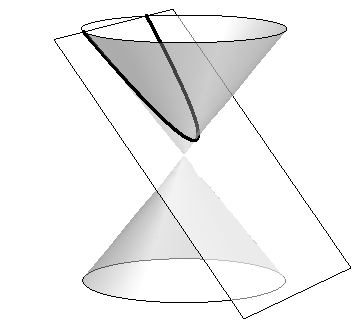
\includegraphics[scale=.25]{figures/conic_parabola}&
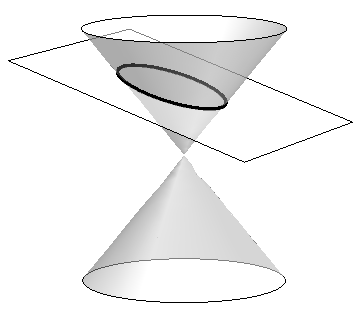
\includegraphics[scale=.25]{figures/conic_ellipse}&
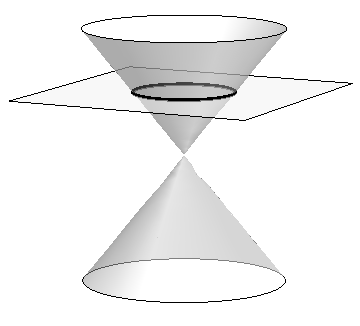
\includegraphics[scale=.25]{figures/conic_circle}&
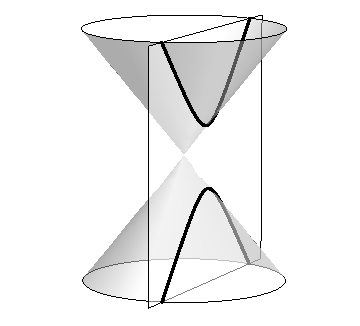
\includegraphics[scale=.25]{figures/conic_hyperbola} \\
\small Parabola &\small Ellipse & \small Circle &  \small Hyperbola
\end{tabular}
\vskip \baselineskip
\noindent%
\begin{tabular}{ccc}
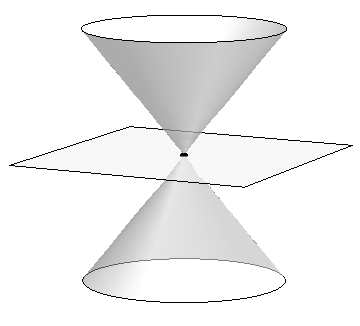
\includegraphics[scale=.25]{figures/conic_singlept}&
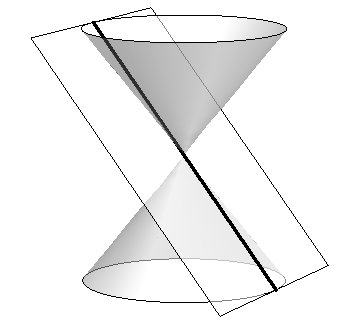
\includegraphics[scale=.25]{figures/conic_oneline}&
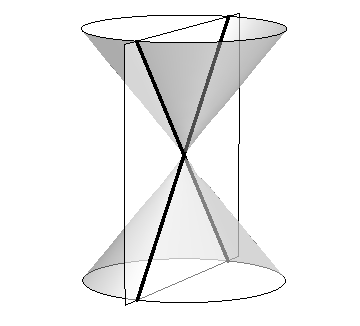
\includegraphics[scale=.25]{figures/conic_crossedlines}
\\
 \small Point& \small Line &\small  Crossed Lines 
\end{tabular}
\captionsetup{type=figure}%
\caption{Conic Sections}\label{fig:nondeg_conic}
\end{minipage}
\vskip\baselineskip

\clearpage

When the plane does contain the origin, three \textbf{degenerate} cones can be formed as shown the bottom row of  Figure \ref{fig:nondeg_conic}: a point, a line, and crossed lines. We focus here on the nondegenerate cases. \index{conic sections}\index{conic sections!degenerate}

While the above geometric constructs define the conics in an intuitive, visual way, these constructs are not very helpful when trying to analyze the shapes algebraically or consider them as the graph of a function. It can be shown that all conics can be defined by the general second--degree equation 
\[
Ax^2+Bxy+Cy^2+Dx+Ey+F=0.
\]
While this algebraic definition has its uses, most find another geometric perspective of the conics more beneficial.

Each nondegenerate conic can be defined as the \textbf{locus}, or set, of points that satisfy a certain distance property. These distance properties can be used to generate an algebraic formula, allowing us to study each conic as the graph of a function.\\

\noindent\textbf{\Large Parabolas}\\
%
%We start with a definition.
%
\definition{def:parabola}{Parabola}
{A \textbf{parabola} is the locus of all points equidistant from a point (called a \textbf{focus}) and a line (called the \textbf{directrix}) that does not contain the focus.
\index{conic sections!parabola}\index{parabola!definition}\index{directrix}\index{focus}
}

\mfigure{.4}{Illustrating the definition of the parabola and establishing an algebraic formula.}{fig:parabola_def}{figures/figparabola_def}
Figure \ref{fig:parabola_def} illustrates this definition. The point halfway between the focus and the directrix is the \textbf{vertex}. The line through the focus, perpendicular to the directrix, is the \textbf{axis of symmetry}, as the portion of the parabola on one side of this line is the mirror--image of the portion on the opposite side.

The definition leads us to an algebraic formula for the parabola. Let $P=(x,y)$ be a point on a parabola whose focus is at $F=(0,p)$ and whose directrix is at $y=-p$. (We'll assume for now that the focus lies on the $y$-axis; by placing the focus $p$ units above the $x$-axis and the directrix $p$ units below this axis, the vertex will be at $(0,0)$.)

We use the Distance Formula to find the distance $d_1$ between $F$ and $P$:
\[
d_1=\sqrt{(x-0)^2+(y-p)^2}.
\]
The distance $d_2$ from $P$ to the directrix is more straightforward:
\[
d_2=y-(-p) = y+p.
\]
These two distances are equal. Setting $d_1=d_2$, we can solve for $y$ in terms of $x$:
	\begin{align*}
	d_1&= d_2 \\
	\sqrt{x^2+(y-p)^2} &= y+p 
	\intertext{Now square both sides.}
	x^2+(y-p)^2 &= (y+p)^2 \\
	x^2+y^2-2yp+p^2 &= y^2+2yp+p^2\\
	x^2 &=4yp\\
	y&= \frac{1}{4p}x^2.
	\end{align*}
	The geometric definition of the parabola has led us to the familiar quadratic function whose graph is a parabola with vertex at the origin. When we allow the vertex to not be at $(0,0)$, we get the following standard form of the parabola.
	
	\keyidea{idea:parabola}{General Equation of a Parabola}
	{\begin{enumerate}
	\item		\textbf{Vertical Axis of Symmetry:} The equation of the parabola with vertex at $(h,k)$ and directrix $y=k-p$ in standard form is 
	\[
	y=\frac{1}{4p}(x-h)^2+k.
	\] 
	The focus is at $(h,k+p)$.
	\item		\textbf{Horizontal Axis of Symmetry:} The  equation of the parabola with vertex at $(h,k)$ and directrix $x=h-p$ in standard form is 
	\[
	x=\frac{1}{4p}(y-k)^2+h.
	\]
	The focus is at $(h+p,k)$.
	\end{enumerate}
	Note: $p$ is not necessarily a positive number.
	\index{parabola!general equation}
	}
	\enlargethispage{2\baselineskip}
	
	\example{ex_conic1}{Finding the equation of a parabola}{
	Give the equation of the parabola with focus at $(1,2)$ and directrix at $y=3$.}
	{The vertex is located halfway between the focus and directrix, so $(h,k) = (1,2.5)$. This gives $p=-0.5$. Using Key Idea \ref{idea:parabola} we have the equation of the parabola as 
	\[
	y=\frac{1}{4(-0.5)}(x-1)^2+2.5 = -\frac12(x-1)^2+2.5.
	\]
	\mfigure{.45}{The parabola described in Example \ref{ex_conic1}.}{fig:conic1}{figures/figconic1}
	The parabola is sketched in Figure \ref{fig:conic1}.
	}\\
	
	\example{ex_conic2}{Finding the focus and directrix of a parabola}{
	Find the focus and directrix of the parabola $x=\frac18y^2-y+1$. The point $(7,12)$ lies on the graph of this parabola; verify that it is equidistant from the focus and directrix.}
	{We need to put the equation of the parabola in its general form. This requires us to complete the square:
	\begin{align*}
	x &= \frac18y^2-y+1 \\
	&= \frac18\big(y^2-8y+8\big)\\
	&=	\frac18\big(y^2-8y+16 -16+8\big)\\
	&=	\frac18\big((y-4)^2 - 8\big)\\
	&=	\frac18(y-4)^2 -1.
	\end{align*}
	Hence the vertex is located at $(-1,4)$.  We have $\frac18=\frac1{4p}$, so $p=2$. We conclude that the focus is located at $(1,4)$ and the directrix is  $x=-3$. The parabola is graphed in Figure \ref{fig:conic2}, along with its focus and directrix.\\
	
\mfigure{.2}{The parabola described in Example \ref{ex_conic2}. The distances from a point on the parabola to the focus and directrix is given.}{fig:conic2}{figures/figconic2}
	
	The point $(7,12)$ lies on the graph and is $7-(-3)=10$ units from the directrix. The distance from $(7,12)$ to the focus is:
	\[
	\sqrt{(7-1)^2 + (12-4)^2} = \sqrt{100}=10.
	\]
	Indeed, the point on the parabola is equidistant from the focus and directrix.
	}\\
	
	\vskip\baselineskip
	\noindent\textbf{\large Reflective Property}
	\vskip\baselineskip
	
	One of the fascinating things about the nondegenerate conic sections is their reflective properties. Parabolas have the following reflective property:
	
	\hskip 20pt \begin{minipage}[t]{.8\linewidth}
	Any ray emanating from the focus that intersects the parabola reflects off along a line perpendicular to the directrix.
	\end{minipage}\\
	\enlargethispage{\baselineskip}
	
	This is illustrated in Figure \ref{fig:conic_reflect}. The following theorem states this more rigorously.
\mfigure{.3}{Illustrating the parabola's reflective property.}{fig:conic_reflect}{figures/figconic_reflect}
	
	\theorem{thm:parabola_reflect}{Reflective Property of the Parabola}
	{Let $P$ be a point on a parabola. The tangent line to the parabola at $P$ makes equal angles with the following two lines:
		\begin{enumerate}
		\item		The line containing $P$ and the focus $F$, and
		\item		The line perpendicular to the directrix through $P$.
		\index{parabola!reflective property}
		\end{enumerate}
	}
	
	Because of this reflective property, paraboloids (the 3D analogue of parabolas) make for useful flashlight reflectors as the light from the bulb, ideally located at the focus, is reflected along parallel rays. Satellite dishes also have paraboloid shapes. Signals coming from satellites effectively approach the dish along parallel rays. The dish then \textit{focuses} these rays at the focus, where the sensor is located.\\
\pagebreak
	
	\noindent\textbf{\Large Ellipses}
	\vskip \baselineskip
	
	\definition{def:ellipse}{Ellipse}
	{An \textbf{ellipse} is the locus of all points whose sum of distances from two fixed points, each a \textbf{focus} of the ellipse, is constant.\index{conic sections!ellipse}\index{ellipse!definition}\index{focus}
	}
	
	An easy way to visualize this construction of an ellipse is to pin both ends of a string to a board. The pins become the foci. Holding a pencil tight against the string places the pencil on the ellipse; the sum of distances from the pencil to the pins is constant: the length of the string. See Figure \ref{fig:ellipse_def}.
	\mfigure{.7}{Illustrating the construction of an ellipse with pins, pencil and string.}{fig:ellipse_def}{figures/figellipse_def}
	
	We can again find an algebraic equation for an ellipse using this geometric definition. Let the foci be located along the $x$-axis, $c$ units from the origin. Let these foci be labelled as $F_1 = (-c,0)$ and $F_2=(c,0)$. Let $P=(x,y)$ be a point on the ellipse. The sum of distances from $F_1$ to $P$ ($d_1$) and from $F_2$ to $P$ ($d_2$) is a constant $d$. That is, $d_1+d_2=d$. Using the Distance Formula, we have 
	\[
	\sqrt{(x+c)^2+y^2} + \sqrt{(x-c)^2+y^2} = d.
	\]
	Using a fair amount of algebra can produce the following equation of an ellipse (note that the equation is an implicitly defined function; it has to be, as an ellipse fails the Vertical Line Test):
	\[
	\frac{x^2}{\left(\frac d2\right)^2} + \frac{y^2}{\left(\frac d2\right)^2-c^2} = 1.
	\]
	This is not particularly illuminating, but by making the substitution $a=d/2$ and $b=\sqrt{a^2-c^2}$, we can rewrite the above equation as 
	\[
	\frac{x^2}{a^2} + \frac{y^2}{b^2} = 1.
	\]
	This choice of $a$ and $b$ is not without reason; as shown in Figure \ref{fig:ellipse_label}, the values of $a$ and $b$ have geometric meaning in the graph of the ellipse. 
\mfigure{.25}{Labelling the significant features of an ellipse.}{fig:ellipse_label}{figures/figellipse_label}
	
	In general, the two foci of an ellipse lie on the \textbf{major axis} of the ellipse, and the midpoint of the segment joining the two foci is the \textbf{center}. The major axis intersects the ellipse at two points, each of which is a \textbf{vertex}. The line segment through the center and perpendicular to the major axis is the \textbf{minor axis}. The ``constant sum of distances'' that defines the ellipse is the length of the major axis, i.e., $2a$.
	
	Allowing for the shifting of the ellipse gives the following standard equations.
	
	\keyidea{idea:ellipse}{Standard Equation of the Ellipse}
	{The equation of an ellipse centered at $(h,k)$ with major axis of length $2a$ and minor axis of length $2b$ in standard form is:
	\begin{enumerate}
	\item	\textbf{Horizontal major axis:} $\ds \frac{(x-h)^2}{a^2}+\frac{(y-k)^2}{b^2}=1.$
	
	\item	\textbf{Vertical major axis:} $\ds \frac{(x-h)^2}{b^2}+\frac{(y-k)^2}{a^2}=1.$
	\end{enumerate}
	The foci lie along the major axis, $c$ units from the center, where $c^2=a^2-b^2$.
	\index{ellipse!standard equation}
	}
	
	\example{ex_conic3}{Finding the equation of an ellipse}{
	Find the general equation of the ellipse graphed in Figure \ref{fig:conic3}.}
	{The center is located at $(-3,1)$. The distance from the center to a vertex is 5 units, hence $a=5$. The minor axis seems to have length 4, so $b=2$. Thus the equation of the ellipse is 
	\[
	\frac{(x+3)^2}{4}+\frac{(y-1)^2}{25} = 1.
	\]
	\mfigure{.65}{The ellipse used in Example \ref{ex_conic3}.}{fig:conic3}{figures/figconic3}
	}\\
	
\example{ex_conic4}{Graphing an ellipse}{
Graph the ellipse defined by $4x^2+9y^2-8x-36y=-4$.}
{It is simple to graph an ellipse once it is in standard form. In order to put the given equation in standard form, we must complete the square with both the $x$ and $y$ terms. We first rewrite the equation by regrouping:
\[
4x^2+9y^2-8x-36y=-4 \quad \Rightarrow \quad (4x^2-8x) + (9y^2-36y) = -4.
\]
Now we complete the squares.
\begin{align*}
(4x^2-8x) + (9y^2-36y) &= -4\\
4(x^2-2x) + 9(y^2-4y) &= -4 \\
4(x^2-2x +1 - 1) + 9(y^2-4y+4-4) &= - 4\\
4\big((x-1)^2-1\big) + 9\big((y-2)^2-4\big) &= -4\\
4(x-1)^2 -4 + 9(y-2)^2-36 &= -4 \\
4(x-1)^2 + 9(y-2)^2 &= 36 \\
\frac{(x-1)^2}{9} + \frac{(y-2)^2}{4} &= 1.
\end{align*}
We see the center of the ellipse is at $(1,2)$. We have $a=3$ and $b=2$; the major axis is horizontal, so the vertices are located at $(-2,2)$ and $(4,2)$. We find $c=\sqrt{9-4} = \sqrt{5}\approx 2.24.$ The foci are located along the major axis, approximately $2.24$ units from the center, at $(1\pm 2.24,2)$. This is all graphed in Figure \ref{fig:conic4}
\mfigure{.3}{Graphing the ellipse in Example \ref{ex_conic4}.}{fig:conic4}{figures/figconic4}.
}\\
\pagebreak

\noindent\textbf{\large Eccentricity}
\vskip\baselineskip

When $a=b$, we have a circle. The general equation becomes 
\[
\frac{(x-h)^2}{a^2} + \frac{(y-k)^2}{a^2} = 1 \quad \Rightarrow (x-h)^2 + (y-k)^2 = a^2,
\]
the familiar equation of the circle centred at $(h,k)$ with radius $a$.  Since $a=b$, $c = \sqrt{a^2-b^2}=0$. The circle has ``two'' foci, but they lie on the same point, the center of the circle. 



Consider Figure \ref{fig:ellipse_ecc}, where several ellipses are graphed with $a=1$. In (a), we have $c=0$ and the ellipse is a circle. As $c$ grows, the resulting ellipses look less and less circular. A measure of this ``noncircularness'' is \textit{eccentricity}.

\mtable{.6}{Understanding the eccentricity of an ellipse.}{fig:ellipse_ecc}{%
\begin{tabular}{c}
\myincludegraphics[scale=.75]{figures/figellipse_ecca}\\
(a)\\
\myincludegraphics[scale=.75]{figures/figellipse_eccb}\\
(b)\\
\myincludegraphics[scale=.75]{figures/figellipse_eccc}\\
(c)\\
\myincludegraphics[scale=.75]{figures/figellipse_eccd}\\
(d)
\end{tabular}
}

\definition{def:eccentricity_ellipse}{Eccentricity of an Ellipse}
{The eccentricity $e$ of an ellipse  is $\ds e=\frac{c}{a}$.
\index{ellipse!eccentricity}\index{eccentricity}
}

The eccentricity of a circle is 0; that is, a circle has no ``noncircularness.'' As $c$ approaches $a$, $e$ approaches 1, giving rise to a very noncircular ellipse, as seen in Figure \ref{fig:ellipse_ecc} (d). 

It was long assumed that planets had circular orbits. This is known to be incorrect; the orbits are elliptical. Earth has an eccentricity of $0.0167$ -- it has a nearly circular orbit.   Mercury's orbit is the most eccentric, with $e=0.2056$. (Pluto's eccentricity is greater, at $e=0.248$, the greatest of all the currently known dwarf planets.) The planet with the most circular orbit is Venus, with $e=0.0068$. The Earth's moon has an eccentricity of $e=0.0549$, also very circular.\\



\noindent \textbf{\large Reflective Property}
\vskip\baselineskip

The ellipse also possesses an interesting reflective property. Any ray emanating from one focus of an ellipse reflects off the ellipse along a line through the other focus, as illustrated in Figure \ref{fig:ellipse_reflect}. This property is given formally in the following theorem.

\mfigure{.2}{Illustrating the reflective property of an ellipse.}{fig:ellipse_reflect}{figures/figellipse_reflect}

\theorem{thm:ellipse_reflect}{Reflective Property of an Ellipse}
{Let $P$ be a point on a ellipse with foci $F_1$ and $F_2$. The tangent line to the ellipse at $P$ makes equal angles with the following two lines:\index{ellipse!reflective property}
\begin{enumerate}
	\item The line through $F_1$ and $P$, and
	\item	The line through $F_2$ and $P$. 
\end{enumerate}
}

This reflective property is useful in optics and is the basis of the phenomena experienced in whispering halls.

\vskip\baselineskip

\pagebreak

\noindent\textbf{\Large Hyperbolas}
\vskip \baselineskip

The definition of a hyperbola is very similar to the definition of an ellipse; we essentially just change the word ``sum'' to ``difference.''

\definition{def:hyperbola}{Hyperbola}
{A \textbf{hyperbola} is the locus of all points where the absolute value of difference of distances from two fixed points, each a focus of the hyperbola, is constant.
\index{conic sections!hyperbola}\index{hyperbola!definition}\index{focus}
}

We do not have a convenient way of visualizing the construction of a hyperbola as we did for the ellipse. The geometric definition does allow us to find an algebraic expression that describes it. It will be useful to define some terms first.

The two foci lie on the \textbf{transverse axis} of the hyperbola; the midpoint of the line segment joining the foci is the \textbf{center} of the hyperbola. The transverse axis intersects the hyperbola at two points, each a \textbf{vertex} of the hyperbola. The line through the center and perpendicular to the transverse axis is the \textbf{conjugate axis.} This is illustrated in Figure \ref{fig:hyperbola_def}. It is easy to show that the constant difference of distances used in the definition of the hyperbola is the distance between the vertices, i.e., $2a$.
\mfigure{.7}{Labelling the significant features of a hyperbola.}{fig:hyperbola_def}{figures/fighyperbola_def}

\keyidea{idea:hyperbola}{Standard Equation of a Hyperbola}
{The equation of a hyperbola centered at $(h,k)$ in standard form is:
\index{hyperbola!standard equation}
\begin{enumerate}
	\item \parbox{120pt}{\textbf{Horizontal Transverse Axis:}} $\ds \frac{(x-h)^2}{a^2} - \frac{(y-k)^2}{b^2} = 1.$
	
	\item	\parbox{120pt}{\textbf{Vertical Transverse Axis:}} $\ds \frac{(y-k)^2}{a^2}-\frac{(x-h)^2}{b^2} = 1.$
\end{enumerate}
The vertices are located $a$ units from the center and the foci are located $c$ units from the center, where $c^2 = a^2+b^2$. 
}

\noindent \textbf{\large Graphing Hyperbolas}
\vskip\baselineskip

Consider the hyperbola $\frac{x^2}9-\frac{y^2}1 = 1$. Solving for $y$, we find $y=\pm\sqrt{x^2/9-1}$. As $x$ grows large, the ``$-1$'' part of the equation for $y$ becomes less significant and $y\approx \pm\sqrt{x^2/9} = \pm x/3$. That is, as $x$ gets large, the graph of the hyperbola looks very much like the lines $y=\pm x/3$. These lines are asymptotes of the hyperbola, as shown in Figure \ref{fig:hyperbola_asy1}.
\mfigure{.45}{Graphing the hyperbola $\frac{x^2}9-\frac{y^2}1 = 1$ along with its asymptotes, $y=\pm x/3$.}{fig:hyperbola_asy1}{figures/fighyperbola_asy1}

This is a valuable tool in sketching. Given the equation of a hyperbola in general form, draw a rectangle centered at $(h,k)$ with sides of length $2a$ parallel to the transverse axis and sides of length $2b$ parallel to the conjugate axis. (See Figure \ref{fig:hyperbola_asy2} for an example with a horizontal transverse axis.) The diagonals of the rectangle lie on the asymptotes. 
\mfigure{.2}{Using the asymptotes of a hyperbola as a graphing aid.}{fig:hyperbola_asy2}{figures/fighyperbola_asy2}

These lines pass through $(h,k)$.  When the transverse axis is horizontal, the slopes are $\pm b/a$; when the transverse axis is vertical, their slopes are $\pm a/b$. This gives equations:

\begin{center}
\begin{tabular}{cc}
\parbox{100pt}{\centering Horizontal \\ Transverse Axis} & \parbox{100pt}{\centering Vertical \\ Transverse Axis} \\ \ \\
$\ds y=\pm\frac ba(x-h)+k$  &$\ds  y=\pm\frac ab(x-h)+k.$
\end{tabular}
\end{center}

\example{ex_conic5}{Graphing a hyperbola}{
Sketch the hyperbola given by $\ds \frac{(y-2)^2}{25}-\frac{(x-1)^2}{4}=1.$}
{The hyperbola is centred at $(1,2)$; $a=5$ and $b=2$. In Figure \ref{fig:conic5} we draw the prescribed rectangle centred at $(1,2)$ along with the asymptotes defined by its diagonals. The hyperbola has a vertical transverse axis, so the vertices are located at $(1,7)$ and $(1,-3)$. This is enough to make a good sketch.
\mfigure{.73}{Graphing the hyperbola in Example \ref{ex_conic5}.}{fig:conic5}{figures/figconic5}

We also find the location of the foci: as $c^2= a^2+b^2$, we have $c=\sqrt{29}\approx 5.4$. Thus the foci are located at $(1,2\pm 5.4)$ as shown in the figure.
}\\

\example{ex_conic6}{Graphing a hyperbola}{
Sketch the hyperbola given by $9x^2-y^2+2y=10.$}
{We must complete the square to put the equation in general form. (We recognize this as a hyperbola since it is a general quadratic equation and the $x^2$ and $y^2$ terms have opposite signs.)

\begin{align*}
9x^2-y^2+2y &=10\\
9x^2- (y^2-2y) &= 10\\
9x^2 - (y^2-2y+1-1) &= 10\\
9x^2 -\big((y-1)^2-1\big) &= 10\\
9x^2 - (y-1)^2 &= 9\\
x^2 - \frac{(y-1)^2}{9} &=1
\end{align*}
\mfigure{.45}{Graphing the hyperbola in Example \ref{ex_conic6}.}{fig:conic6}{figures/figconic6}

We see the hyperbola is centred at $(0,1)$, with a horizontal transverse axis, where $a=1$ and $b=3$. The appropriate rectangle is sketched in Figure \ref{fig:conic6} along with the asymptotes of the hyperbola. The vertices are located at $(\pm 1,1)$. We have $c=\sqrt{10}\approx 3.2$, so the foci are located at $(\pm 3.2,1)$ as shown in the figure.
}\\
\clearpage

\noindent\textbf{\large Eccentricity}
\vskip\baselineskip

\definition{def:hyperbola_eccentricity}{Eccentricity of a Hyperbola}
{The eccentricity of a hyperbola is $\ds e=\frac ca$.\index{hyperbola!eccentricity}\index{eccentricity}
}

\mtable{.5}{Understanding the eccentricity of a hyperbola.}{fig:hyperbola_ecc}{%
\begin{tabular}{c}
\myincludegraphics{figures/fighyperbola_ecca} \\
(a)\rule[-15pt]{0pt}{25pt}\\
\myincludegraphics{figures/fighyperbola_eccb} \\
(b)\rule[-15pt]{0pt}{25pt}\\
\myincludegraphics{figures/fighyperbola_eccc} \\
(c)\rule[-15pt]{0pt}{25pt}\\
\myincludegraphics{figures/fighyperbola_eccd} \\
(d)\rule[-15pt]{0pt}{25pt}
\end{tabular}
}
Note that this is the definition of eccentricity as used for the ellipse.  When $c$ is close in value to $a$ (i.e., $e\approx 1$), the hyperbola is very narrow (looking almost like crossed lines). Figure \ref{fig:hyperbola_ecc} shows hyperbolas centered at the origin with $a=1$. The graph in (a) has $c=1.05$, giving an eccentricity of $e=1.05$, which is close to 1. As $c$ grows larger, the hyperbola widens and begins to look like parallel lines, as shown in part (d) of the figure.\\

\noindent\textbf{\large Reflective Property}
\vskip\baselineskip

Hyperbolas share a similar reflective property with ellipses. However, in the case of a hyperbola, a ray emanating from a focus that intersects the hyperbola reflects along a line containing the other focus, but moving \textit{away} from that focus. This is illustrated in Figure \ref{fig:hyperbola_reflect} (on the next page). Hyperbolic mirrors are commonly used in telescopes because of this reflective property. It is stated formally in the following theorem.

\theorem{thm:reflective_hyperbola}{Reflective Property of Hyperbolas}
{Let $P$ be a point on a hyperbola with foci $F_1$ and $F_2$. The tangent line to the hyperbola at $P$ makes equal angles with the following two lines:\index{hyperbola!reflective property}
	\begin{enumerate}
		\item The line through $F_1$ and $P$, and
		\item	The line through $F_2$ and $P$.
	\end{enumerate}
}\\

\medskip

\noindent\textbf{\large Location Determination}
\vskip\baselineskip

Determining the location of a known event has many practical uses (locating the epicenter of an earthquake, an airplane crash site, the position of the person speaking in a large room, etc.).  

To determine the location of an earthquake's epicenter, seismologists use \textit{trilateration} (not to be confused with \textit{triangulation}). A seismograph allows one to determine how far away the epicenter was; using three separate readings, the location of the epicenter can be approximated.

A key to this method is knowing distances. What if this information is not available? Consider three microphones at positions $A$, $B$ and $C$ which all record a noise (a person's voice, an explosion, etc.) created at unknown location $D$. The microphone does not ``know'' when the sound was \textit{created}, only when the sound was \textit{detected}. How can the location be determined in such a situation?

If each location has a clock set to the same time, hyperbolas can be used to determine the location. Suppose the microphone at position $A$ records the sound at exactly 12:00, location $B$ records the time exactly 1 second later, and location $C$ records the noise exactly 2 seconds after that. We are interested in the \textit{difference} of times. Since the speed of sound is approximately 340 m/s, we can conclude quickly that the sound was created 340 meters closer to position $A$ than position $B$. If $A$ and $B$ are a known distance apart (as shown in Figure \ref{fig:hyperbola_locate} (a)), then we can determine a hyperbola on which $D$ must lie. 

The ``difference of distances'' is 340; this is also the distance between vertices of the hyperbola. So we know $2a= 340$. Positions $A$ and $B$ lie on the foci, so $2c=1000$. From this we can find $b\approx 470$ and can sketch the hyperbola, given in part (b) of the figure. We only care about the side closest to $A$. (Why?)

We can also find the hyperbola defined by positions $B$ and $C$. In this case, $2a = 680$ as the sound travelled an extra 2 seconds to get to $C$. We still have $2c=1000$, centring this hyperbola at $(-500,500)$. We find $b\approx 367$. This hyperbola is sketched in part (c) of the figure. The intersection point of the two graphs is the location of the sound, at approximately $(188,-222.5)$.\\

\mfigure{.82}{Illustrating the reflective property of a hyperbola.}{fig:hyperbola_reflect}{figures/fighyperbola_reflect}

\vskip 10pt
\noindent%\hskip-160pt
\begin{minipage}{\textwidth+150pt}
\centering
\begin{tabular}{ccccc}
\myincludegraphics{figures/fighyperbola_locate1}  &\hskip 15pt & \myincludegraphics{figures/fighyperbola_locate2} &\hskip 15pt  & \myincludegraphics{figures/fighyperbola_locate3}  \\ 
(a) & & (b) & & (c) 
\end{tabular}
\captionsetup{type=figure}
\caption{Using hyperbolas in location detection.}\label{fig:hyperbola_locate}
\end{minipage}\\

\enlargethispage{2\baselineskip}
This chapter explores curves in the plane, in particular curves that cannot be described by functions of the form $y=f(x)$. In this section, we learned of ellipses and hyperbolas that are defined implicitly, not explicitly. In the following sections, we will learn completely new ways of describing curves in the plane, using \emph{parametric equations} and \emph{polar coordinates}, then study these curves using calculus techniques.


\printexercises{exercises/09_01_exercises}

\section{Parametric Equations}\label{sec:param_eqs}

We are familiar with sketching  shapes, such as parabolas, by following this basic procedure:

\begin{center}
\begin{tikzpicture}[>=latex]
\draw (0,0) node (A) [align=center] {Choose \\$x$} 
      (3,0) node[align=center] (B) {Use a function\\ $f$ to find $y$\\$\big(y=f(x)\big)$}
			(6.25,0) node [align=center] (C) {Plot point \\ $(x,y)$};
\draw [->](A) --(B);
\draw [->](B) -- (C);
\end{tikzpicture}
\end{center}

The \textbf{rectangular equation} $y=f(x)$ works well for some shapes like a parabola with a vertical axis of symmetry, but in the previous section we encountered several shapes that could not be sketched in this manner. (To plot an ellipse using the above procedure, we need to plot the ``top'' and ``bottom'' separately.)\index{curve!rectangular equation}

In this section we introduce a new sketching procedure:

\begin{center}
\begin{tikzpicture}[>=latex]
\draw (0,0) node (A) [align=center] {Choose \\$t$} 
      (3,1) node[align=center] (B1) {Use a function\\ $f$ to find $x$\\$\big(x=f(t)\big)$}
			(3,-1) node[align=center] (B2) {Use a function\\ $g$ to find $y$\\$\big(y=g(t)\big)$}
			(6.25,0) node [align=center] (C) {Plot point \\ $(x,y)$};
\draw [->](A) --(B1);
\draw [->](A) --(B2);
\draw [->](B1) -- (C);
\draw [->](B2) -- (C);
\end{tikzpicture}
\end{center}

Here, $x$ and $y$ are found separately but then plotted together. This leads us to a definition.

\definition{def:param_eq}{Parametric Equations and Curves}
{Let $f$ and $g$ be continuous functions on an interval $I$. The set of all points $\big(x,y\big) = \big(f(t),g(t)\big)$ in the Cartesian plane, as $t$ varies over $I$, is the \textbf{graph} of the \textbf{parametric equations} $x=f(t)$ and $y=g(t)$, where $t$ is the \textbf{parameter}. A \textbf{curve} is a graph along with the parametric equations that define it.
\index{curve!parametrically defined}\index{parametric equations!definition}
}

This is a formal definition of the word \textit{curve}. When a curve lies in a plane (such as the Cartesian plane), it is often referred to as a \textbf{plane curve}. Examples will help us understand the concepts introduced in the definition.\\

\example{ex_pareq1}{Plotting parametric functions}{ \\
Plot the graph of the parametric equations $x=t^2$, $y=t+1$ for $t$ in $[-2,2]$.}
{We plot the graphs of parametric equations in much the same manner as we plotted graphs of functions like $y=f(x)$: we make a table of values, plot points, then connect these points with a ``reasonable'' looking curve. Figure \ref{fig:pareq1}(a) shows such a table of values; note how we have 3 columns.

The points $(x,y)$ from the table are plotted in Figure \ref{fig:pareq1}(b). The points have been connected with a smooth curve. Each point has been labeled with its corresponding $t$-value. These values, along with the two arrows along the curve, are used to indicate the \textbf{orientation} of the graph. This information helps us determine the direction in which the graph is ``moving.''
%\mtable{.85}{A table of values of the parametric equations in Example \ref{ex_pareq1}.}{fig:pareq1table}{%
%\begin{tabular}{rrr}
%$t$ & $x$ & $y$ \\ \hline
%$-2$ & \phantom{$-$}4 & $-1$ \\  $-1$ & 1 & 0 \\ 0 & 0 & 1 \\ 1 & 1 & 2 \\ 2 & 4 & 3
%\end{tabular}}
%\mfigure{.65}{Sketching the graph of the parametric equations in Example \ref{ex_pareq1}.}{fig:pareq1}{figures/figpareq1}
\mtable{.65}{A table of values of the parametric equations in Example \ref{ex_pareq1} along with a sketch of their graph.}{fig:pareq1}{%
\begin{tabular}{c}
\begin{tabular}{rrr}
$t$ & $x$ & $y$ \\ \hline
$-2$ & \phantom{$-$}4 & $-1$ \\  $-1$ & 1 & 0 \\ 0 & 0 & 1 \\ 1 & 1 & 2 \\ 2 & 4 & 3
\end{tabular}\\ \\
(a)\\
\myincludegraphics{figures/figpareq1}\\
(b)
\end{tabular}}
}\\

We often use the letter $t$ as the parameter as we often regard $t$ as representing \textit{time}. Certainly there are many contexts in which the parameter is not time, but it can be helpful to think in terms of time as one makes sense of parametric plots and their orientation (for instance, ``At time $t=0$ the position is $(1,2)$ and at time $t=3$ the position is $(5,1)$.'').
\\

\example{ex_pareq2}{Plotting parametric functions}{ \\ Sketch the graph of the parametric equations $x=\cos^2t$, $y=\cos t+1$ for $t$ in $[0,\pi]$.}
{We again start by making a table of values in Figure \ref{fig:pareq2}(a), then plot the points $(x,y)$ on the Cartesian plane in Figure \ref{fig:pareq2}(b).
%\mtable{.46}{A table of values of the parametric equations in Example \ref{ex_pareq2}.}{fig:pareq2_table}{%
%\begin{tabular}{ccc}
%$t$ & $x$ & $y$ \\ \hline
%0 & 1 & 2 \\
%$\pi/4$ & $1/2$ & $1+\sqrt{2}/2$ \\
%$\pi/2$ & 0 & 1\\
%$3\pi/4$ & $1/2$ & $1-\sqrt{2}/2$ \\
%$\pi$ & 1 & 0
%\end{tabular}
%}
%\mfigure{.28}{Sketching the graph of the parametric equations in Example \ref{ex_pareq2}.}{fig:pareq2}{figures/figpareq2}
\mtable{.45}{A table of values of the parametric equations in Example \ref{ex_pareq2} along with a sketch of their graph.}{fig:pareq2}{%
\begin{tabular}{c}
\begin{tabular}{ccc}
$t$ & $x$ & $y$ \\ \hline
0 & 1 & 2 \\
$\pi/4$ & $1/2$ & $1+\sqrt{2}/2$ \\
$\pi/2$ & 0 & 1\\
$3\pi/4$ & $1/2$ & $1-\sqrt{2}/2$ \\
$\pi$ & 1 & 0
\end{tabular}\\ \\
(a)\\
\myincludegraphics{figures/figpareq2}\\
(b)
\end{tabular}
}

It is not difficult to show that the curves in Examples \ref{ex_pareq1} and \ref{ex_pareq2} are portions of the same parabola. While the \textit{parabola} is the same, the \textit{curves} are different. In Example \ref{ex_pareq1}, if we let $t$ vary over all real numbers, we'd obtain the entire parabola. In this example, letting $t$ vary over all real numbers would still produce the same graph; this portion of the parabola would be traced, and re--traced, infinitely. The orientation shown in Figure \ref{fig:pareq2} shows the orientation on $[0,\pi]$, but this orientation is reversed on $[\pi,2\pi]$.

These examples begin to illustrate the powerful nature of parametric equations. Their graphs are far more diverse than the graphs of functions produced by ``$y=f(x)$'' functions.
}\\

\noindent\textbf{Technology Note:} Most graphing utilities can graph functions given in parametric form. Often the word ``parametric'' is abbreviated as ``PAR'' or ``PARAM'' in the  options. The user usually needs to determine the graphing window (i.e, the minimum and maximum $x$- and $y$-values), along with the values of $t$ that are to be plotted. The user is often prompted to give a $t$ minimum, a $t$ maximum, and a ``$t$-step'' or ``$\Delta t$.'' Graphing utilities effectively plot parametric functions just as we've shown here: they plots lots of points. A smaller $t$-step plots more points, making for a smoother graph (but may take longer). In Figure \ref{fig:pareq1}, the $t$-step is 1; in Figure \ref{fig:pareq2}, the $t$-step is $\pi/4$.\\

One nice feature of parametric equations is that their graphs are easy to shift. While this is not too difficult in the ``$y=f(x)$'' context, the resulting function can look rather messy. (Plus, to shift to the right by two, we replace $x$ with $x-2$, which is counter--intuitive.) The following example demonstrates this.\\

\example{ex_pareq3}{Shifting the graph of parametric functions}{ Sketch the graph of the parametric equations $x=t^2+t$, $y=t^2-t$.  Find new parametric equations that shift this graph to the right 3 places and down 2.}
{The graph of the parametric equations is given in Figure \ref{fig:pareq3} (a). It is a parabola with a axis of symmetry along the line $y=x$; the vertex is at $(0,0)$. 

In order to shift the graph to the right 3 units, we need to increase the $x$-value by 3 for every point. The straightforward way to accomplish this is simply to add 3 to the function defining $x$: $x = t^2+t+3$. To shift the graph down by 2 units, we wish to decrease each $y$-value by 2, so we subtract 2 from the function defining $y$: $y = t^2-t-2$. Thus our parametric equations for the shifted graph are $x=t^2+t+3$, $y=t^2-t-2$. This is graphed in Figure \ref{fig:pareq3} (b). Notice how the vertex is now at $(3,-2)$. 


Because the $x$- and $y$-values of a graph are determined independently, the graphs of parametric functions often possess features not seen on ``$y=f(x)$'' type graphs. The next example demonstrates how such graphs can arrive at the same point more than once.

\mtable{.7}{Illustrating how to shift graphs in Example \ref{ex_pareq3}.}{fig:pareq3}{%
\begin{tabular}{cc}
\myincludegraphics{figures/figpareq3a}\\
(a) \\
\myincludegraphics{figures/figpareq3b}\\
(b)
\end{tabular}
}
}\\

\example{ex_pareq4}{Graphs that cross themselves}{ Plot the parametric functions $x=t^3-5t^2+3t+11$ and $y=t^2-2t+3$ and determine the $t$-values where the graph crosses itself.}
{Using the methods developed in this section, we again plot points and graph the parametric equations as shown in Figure \ref{fig:pareq4}. It appears that the graph crosses itself at the point $(2,6)$, but we'll need to analytically determine this.
\mfigure{.3}{A graph of the parametric equations from Example \ref{ex_pareq4}.}{fig:pareq4}{figures/figpareq4}

We are looking for two different values, say, $s$ and $t$, where $x(s) = x(t)$ and $y(s) = y(t)$. That is, the $x$-values are the same precisely when the $y$-values are the same. This gives us a system of 2 equations with 2 unknowns:

$$\begin{array}{c} s^3-5s^2+3s+11 = t^3-5t^2+3t+11\rule[-7pt]{0pt}{10pt}\\
								s^2-2s+3 = t^2-2t+3
	\end{array}$$

Solving this system is not trivial but involves only algebra. Using the quadratic formula, one can solve for $t$ in the second equation and find that $\ds t = 1\pm \sqrt{s^2-2s+1}$. This can be substituted into the first equation, revealing that the graph crosses itself at $t=-1$ and $t=3$. We confirm our result by computing $x(-1) = x(3)=2$ and $y(-1) = y(3) = 6$. 
}\\

\noindent\textbf{\large Converting between rectangular and parametric equations}
\vskip \baselineskip

It is sometimes useful to rewrite equations in rectangular form (i.e., $y=f(x)$) into parametric form, and vice--versa. Converting from rectangular to parametric can be very simple: given $y=f(x)$, the parametric equations $x=t$, $y=f(t)$ produce the same graph. As an example, given $y=x^2$, the parametric equations $x=t$, $y=t^2$ produce the familiar parabola. However, other parametrizations can be used. The following example demonstrates one possible alternative.\\

\example{ex_pareq5}{Converting from rectangular to parametric}{
Consider $y=x^2$. Find parametric equations $x=f(t)$, $y=g(t)$ for the parabola where $t=\frac{dy}{dx}$. That is, $t=a$ corresponds to the point on the graph whose tangent line has slope $a$.}
{We start by computing $\frac{dy}{dx}$: $y\primeskip' = 2x$. Thus we set $t=2x$. We can solve for $x$ and find $x= t/2$. Knowing that $y=x^2$, we have $y= t^2/4$. Thus parametric equations for the parabola $y=x^2$ are $$x=t/2 \quad y=t^2/4.$$
To find the point where the tangent line has a slope of $-2$, we set $t=-2$. This gives the point $(-1, 1)$. We can verify that the slope of the line tangent to the curve at this point indeed has a slope of $-2$.
}\\

We sometimes chose the parameter to accurately model physical behavior.\\

\example{ex_pareq6}{Converting from rectangular to parametric}{
An object is fired from a height of 0ft and lands 6 seconds later, 192ft away. Assuming ideal projectile motion, the height, in feet, of the object can be described by $h(x) = -x^2/64+3x$, where $x$ is the distance in feet from the initial location. (Thus $h(0) = h(192) = 0$ft.) Find parametric equations $x=f(t)$, $y=g(t)$ for the path of the projectile where $x$ is the horizontal distance the object has traveled at time $t$ (in seconds) and $y$ is the height at time $t$.
}
{Physics tells us that the horizontal motion of the projectile is linear; that is, the horizontal speed of the projectile is constant. Since the object travels 192ft in 6s, we deduce that the object is moving horizontally at a rate of 32ft/s, giving the equation $x=32t$. As $y=-x^2/64+3x$, we find $y= -16t^2+96t$. We can quickly verify that $y\primeskip''=-32$ft/s$^2$, the acceleration due to gravity, and that the projectile reaches its maximum at $t=3$, halfway along its path.

These parametric equations make certain determinations about the object's location easy: 2 seconds into the flight the object is at the point $\big(x(2),y(2)\big) = \big(64,128\big)$. That is, it has traveled horizontally 64ft and is at a height of 128ft, as shown in Figure \ref{fig:pareq6}.
\mfigure{.7}{Graphing projectile motion in Example \ref{ex_pareq6}.}{fig:pareq6}{figures/figpareq6}
}\\

It is  sometimes necessary to convert given parametric equations into rectangular form. This can be decidedly more difficult, as some ``simple'' looking parametric equations can have very ``complicated'' rectangular equations. This conversion is often referred to as ``eliminating the parameter,'' as we are looking for a relationship between $x$ and $y$ that does not involve the parameter $t$.\\

\example{ex_pareq7}{Eliminating the parameter}{
Find a rectangular equation for the curve described by $$ x= \frac{1}{t^2+1}\quad \text{and}\quad y=\frac{t^2}{t^2+1}.$$ }
{There is not a set way to eliminate a parameter. One method is to solve for $t$ in one equation and then substitute that value in the second. We use that technique here, then show a second, simpler method.

Starting with $x= 1/(t^2+1)$, solve for $t$: $ t = \pm\sqrt{1/x-1}$. Substitute this value for $t$ in the equation for $y$:
\begin{align*}
 y &= \frac{t^2}{t^2 +1} \\
		&= \frac{1/x-1}{1/x-1+1} \\
		&= \frac{1/x - 1}{1/x} \\
		&= \left(\frac1x-1\right)\cdot x \\
		&= 1-x.
\end{align*}

\mfigure{.3}{Graphing parametric and rectangular equations for a graph in Example \ref{ex_pareq7}.}{fig:pareq7}{figures/figpareq7}
Thus $y=1-x$. One may have recognized this earlier by manipulating the equation for $y$:
$$y = \frac{t^2}{t^2+1} = 1-\frac{1}{t^2+1} = 1-x.$$ This is a shortcut that is very specific to this problem; sometimes shortcuts exist and are worth looking for.

We should be careful to limit the domain of the function $y=1-x$. The parametric equations limit $x$ to values in $(0,1]$, thus to produce the same graph we should limit the domain of $y=1-x$ to the same. 

The graphs of these functions is given in Figure \ref{fig:pareq7}. The portion of the graph defined by the parametric equations is given in a thick line; the graph defined by $y=1-x$ with unrestricted domain is given in a thin line.
}\\

\example{ex_pareq8}{Eliminating the parameter}{
Eliminate the parameter in $x=4\cos t+3$, $y= 2\sin t+1$}
{We should not try to solve for $t$ in this situation as the resulting algebra/trig would be messy. Rather, we solve for $\cos t$ and $\sin t$ in each equation, respectively. This gives $$\cos t = \frac{x-3}{4} \quad \text{and}\quad \sin t=\frac{y-1}{2}.$$
The Pythagorean Theorem gives $\cos^2t+\sin^2t=1$, so:
\begin{align*}
\cos^2t+\sin^2t &=1 \\
\left(\frac{x-3}{4}\right)^2 +\left(\frac{y-1}{2}\right)^2 &=1\\
\frac{(x-3)^2}{16}+\frac{(y-1)^2}{4} &=1
\end{align*}
\mfigure{.6}{Graphing the parametric equations $x=4\cos t+3$, $y=2\sin t+1$ in Example \ref{ex_pareq8}.}{fig:pareq8}{figures/figpareq8} 
This final equation should look familiar -- it is the equation of an ellipse! Figure \ref{fig:pareq8} plots the parametric equations, demonstrating that the graph is indeed of an ellipse with a horizontal major axis and center at $(3,1)$. 
}\\

The Pythagorean Theorem can also be used to identify parametric equations for hyperbolas. We give the parametric equations for ellipses and hyperbolas in the following Key Idea.

%\keyidea{idea:par_ellipse}{Parametric Equations for Ellipses}
%{The parametric equations 
%$$ x=a\cos t+h, \quad y=b\sin t+k$$ define an ellipse with horizontal axis of length $2a$ and vertical axis of length $2b$, centered at $(h,k)$.
%\index{ellipse!parametric equations}%\\
%}
%
%\keyidea{idea:par_hyperbola}{Parametric Equations for Hyperbolas}
%{The parametric equations
%$$ x= a\tan t+h,\quad y=\pm b\sec t+k$$ define a hyperbola with vertical transverse axis centered at $(h,k)$, and 
%$$ x=\pm a\sec t+h, \quad y=b\tan t + k$$ defines a hyperbola with horizontal transverse axis. Each has asymptotes at $y=\pm b/a(x-h)+k$.
%\index{hyperbola!parametric equations}
%}

\keyidea{idea:par_ellipse_hyperbola}{Parametric Equations of Ellipses and Hyperbolas}
{\begin{itemize}
	\item The parametric equations 
$$ x=a\cos t+h, \quad y=b\sin t+k$$ define an ellipse with horizontal axis of length $2a$ and vertical axis of length $2b$, centered at $(h,k)$.
\index{ellipse!parametric equations}
	\item The parametric equations
$$ x= a\tan t+h,\quad y=\pm b\sec t+k$$ define a hyperbola with vertical transverse axis centered at $(h,k)$, and 
$$ x=\pm a\sec t+h, \quad y=b\tan t + k$$ defines a hyperbola with horizontal transverse axis. Each has asymptotes at $y=\pm b/a(x-h)+k$.
\index{hyperbola!parametric equations}
\end{itemize}
}
%%%%% End with this??
%%%%%
\pagebreak

\noindent\textbf{\large Special Curves}
\vskip\baselineskip

Figure \ref{fig:pareq_special} gives a small  gallery of ``interesting'' and ``famous'' curves along with parametric equations that produce them. Interested readers can begin learning more about these curves through internet searches.

One might note a feature shared by two of these graphs: ``sharp corners,'' or \textbf{cusps}. We have seen graphs with cusps before and determined that such functions are not differentiable at these points. This leads us to a definition.

%\noindent
%\begin{figure}%{\linewidth}
%\centering
%\begin{tabular}{cc}
\mtable{.5}{A gallery of interesting planar curves.}{fig:pareq_special}{%
\begin{tabular}{c}
\myincludegraphics{figures/figplanecurve1} \\
\parbox{150pt}{\centering Astroid\\ $x=\cos^3 t$\\ $y=\sin^3t$}\\ \\
 \myincludegraphics{figures/figplanecurve2} \\
 \parbox{150pt}{\centering Rose Curve\\ $x=\cos(t)\sin(4t)$\\ $y=\sin(t)\sin(4t)$}\\ \\
\myincludegraphics{figures/figplanecurve3} \\
\parbox{150pt}{\centering Hypotrochoid\\ $x=2\cos(t)+5\cos(2t/3)$\\$y=2\sin(t)-5\sin(2t/3)$} \\ \\
 \myincludegraphics{figures/figplanecurve4} \\
 \parbox{150pt}{\centering Epicycloid\\ $x=4\cos(t)-\cos(4t)$\\$y=4\sin(t)-\sin(4t)$}
\end{tabular}
}
%\caption{A gallery of interesting planar curves.}\label{fig:pareq_special}
%\end{figure}

\definition{def:smooth}{Smooth}
{A curve $C$ defined by $x=f(t)$, $y=g(t)$ is \textbf{smooth} on an interval $I$ if $\fp$ and $g\primeskip'$ are continuous on $I$ and not simultaneously 0 (except possibly at the endpoints of $I$). A curve is \textbf{piecewise smooth} on $I$ if $I$ can be partitioned into subintervals where $C$ is smooth on each subinterval.
\index{curve!smooth}\index{smooth curve}\index{cusp}
}

Consider the astroid, given by $x=\cos^3t$, $y=\sin^3t$. Taking derivatives, we have:
$$x\primeskip' = -3\cos^2t\sin t\quad \text{and}\quad y\primeskip' = 3\sin^2t\cos t.$$
It is clear that each is 0 when $t=0,\ \pi/2,\ \pi,\ldots$. Thus the astroid is not smooth at these points, corresponding to the cusps seen in the figure.


We demonstrate this once more.\\

\example{ex_pareq9}{Determine where a curve is not smooth}{
Let a curve $C$ be defined by the parametric equations $x=t^3-12t+17$ and $y=t^2-4t+8$. Determine the points, if any, where it is not smooth.}
{We begin by taking derivatives. 
$$x\primeskip' = 3t^2-12,\quad y\primeskip' = 2t-4.$$
We set each equal to 0:
$$\begin{array}{l}x\primeskip' = 0 \Rightarrow 3t^2-12=0 \Rightarrow t=\pm 2\\
  y\primeskip'=0 \Rightarrow 2t-4 = 0 \Rightarrow t=2
	\end{array}
	$$
We see at $t=2$ both $x\primeskip'$ and $y\primeskip'$ are 0; thus $C$ is not smooth at $t=2$, corresponding to the point $(1,4)$. The curve is graphed in Figure \ref{fig:pareq9}, illustrating the cusp at $(1,4)$.
}\\

If a curve is not smooth at $t=t_0$, it means that $x\primeskip'(t_0)=y\primeskip'(t_0)=0$ as defined. This, in turn, means that rate of change of $x$ (and $y$) is 0; that is, at that instant, neither $x$ nor $y$ is changing. If the parametric equations describe the path of some object, this means the object is at rest at $t_0$. An object at rest can make a ``sharp'' change in direction, whereas moving objects tend to change direction in a ``smooth'' fashion.

One should be careful to note that a ``sharp corner'' does not have to occur when a curve is not smooth. For instance, one can verify that $x=t^3$, $y=t^6$ produce the familiar $y=x^2$ parabola. However, in this parametrization, the curve is not smooth. A particle traveling along the parabola according to the given parametric equations comes to rest at $t=0$, though no sharp point is created.\\

Our previous experience with cusps taught us that a function was not differentiable at a cusp. This can lead us to wonder about derivatives in the context of parametric equations and the application of other calculus concepts. Given a curve defined parametrically, how do we find the slopes of tangent lines? Can we determine concavity? We explore these concepts and more in the next section.

\mfigure{.8}{Graphing the curve in Example \ref{ex_pareq9}; note it is not smooth at $(1,4)$.}{fig:pareq9}{figures/figpareq9}

\printexercises{exercises/09_02_exercises}

\section{Calculus and Parametric Equations}\label{sec:par_calc}

The previous section defined curves based on parametric equations. In this section we'll employ the techniques of calculus to study these curves.

We are still interested in lines tangent to points on a curve. They describe how the $y$-values are changing with respect to the $x$-values, they are useful in making approximations, and they indicate instantaneous direction of travel.

The slope of the tangent line is still $\frac{dy}{dx}$, and the Chain Rule allows us to calculate this in the context of parametric equations. If $x=f(t)$ and $y=g(t)$, the Chain Rule states that 
\[
\frac{dy}{dt} = \frac{dy}{dx}\cdot\frac{dx}{dt}.
\]
Solving for $\frac{dy}{dx}$, we get 
\[
\frac{dy}{dx} = \frac{dy}{dt}\Bigg/\frac{dx}{dt} = \frac{g\primeskip'(t)}{\fp(t)},
\]
provided that $\fp(t)\neq 0$. This is important so we label it a Key Idea.

\keyidea{idea:dydxpar}{Finding $\frac{dy}{dx}$ with Parametric Equations.}
{Let $x=f(t)$ and $y=g(t)$, where $f$ and $g$ are differentiable on some open interval $I$ and $\fp(t)\neq 0$ on $I$. Then \index{parametric equations!finding $\frac{dy}{dx}$}\index{derivative!parametric equations}
\[
\frac{dy}{dx} = \frac{g\primeskip'(t)}{\fp(t)}.
\]
}

We use this to define the tangent line.

\definition{def:tangent_par}{Tangent and Normal Lines}
{Let a curve $C$ be parametrized by $x=f(t)$ and $y=g(t)$, where $f$ and $g$ are differentiable functions on some interval $I$ containing $t=t_0$. The \textbf{tangent line} to $C$ at $t=t_0$ is the line through $\big(f(t_0),g(t_0)\big)$ with slope $m=g\primeskip'(t_0)/\fp(t_0)$, provided $\fp(t_0)\neq 0$.\\

The \textbf{normal line} to $C$ at $t=t_0$ is the line through $\big(f(t_0),g(t_0)\big)$ with slope $m=-\fp(t_0)/g\primeskip'(t_0)$, provided $g\primeskip'(t_0)\neq 0$.\index{tangent line}\index{normal line}\index{parametric equations!tangent line}\index{parametric equations!normal line}
}

The definition leaves two special cases to consider. When the tangent line is horizontal, the normal line is undefined by the above definition as $g\primeskip'(t_0)=0$. Likewise, when the normal line is horizontal, the tangent line is undefined. It seems reasonable that these lines be defined (one can draw a line tangent to the ``right side'' of a circle, for instance), so we add the following to the above definition.

	
\begin{enumerate}
	\item If the tangent line at $t=t_0$ has a slope of 0, the normal line to $C$ at $t=t_0$ is the line $x=f(t_0)$.
	\item		If the normal line at $t=t_0$ has a slope of 0, the tangent line to $C$ at $t=t_0$ is the line $x=f(t_0)$.
	\end{enumerate}
	
\example{ex_parcalc1}{Tangent and Normal Lines to Curves}{
Let $x=5t^2-6t+4$ and $y=t^2+6t-1$, and let $C$ be the curve defined by these equations.
\begin{enumerate}
	\item Find the equations of the tangent and normal lines to $C$ at $t=3$.
	\item	Find where $C$ has vertical and horizontal tangent lines.
\end{enumerate}
	}
	{\begin{enumerate}
		\item We start by computing $\fp(t) = 10t-6$ and $g\primeskip'(t) =2t+6$. Thus 
		\[
		\frac{dy}{dx} = \frac{2t+6}{10t-6}.
		\]
		Make note of something that might seem unusual: $\frac{dy}{dx}$ is a function of $t$, not $x$. Just as points on the curve are found in terms of $t$, so are the slopes of the tangent lines.
		
		The point on $C$ at $t=3$ is $(31,26)$. The slope of the tangent line is $m=1/2$ and the slope of the normal line is $m=-2$. Thus,
		\begin{itemize}
			\item the equation of the tangent line is $\ds y=\frac12(x-31)+26$, and
			\item	the equation of the normal line is $\ds y=-2(x-31)+26$.
		\end{itemize}
		This is illustrated in Figure \ref{fig:parcalc1}.
		\mfigure{.5}{Graphing tangent and normal lines in Example \ref{ex_parcalc1}.}{fig:parcalc1}{figures/figparcalc1}
		
		\item		To find where $C$ has a horizontal tangent line, we set $\frac{dy}{dx}=0$ and solve for $t$. In this case, this amounts to setting $g\primeskip'(t)=0$ and solving for $t$ (and making sure that $\fp(t)\neq 0$). 
		\[
		g\primeskip'(t)=0 \quad \Rightarrow \quad 2t+6=0 \quad \Rightarrow \quad t=-3.
		\]
		The point on $C$ corresponding to $t=-3$ is $(67,-10)$; the tangent line at that point is horizontal (hence with equation $y=-10$).
		
		To find where $C$ has a vertical tangent line, we find where it has a horizontal normal line, and set $-\frac{\fp(t)}{g\primeskip'(t)}=0$. This amounts to setting $\fp(t)=0$ and solving for $t$ (and making sure that $g\primeskip'(t)\neq 0$). 
		\[
		\fp(t)=0 \quad \Rightarrow \quad 10t-6=0 \quad \Rightarrow \quad t=0.6.
		\]
		The point on $C$ corresponding to $t=0.6$ is $(2.2,2.96)$. The tangent line at that point is $x=2.2$.
	
		The points where the tangent lines are vertical and horizontal are indicated on the graph in Figure \ref{fig:parcalc1}.
		\end{enumerate}
		\vskip-\baselineskip
	}\\
	
	\example{ex_parcalc2}{Tangent and Normal Lines to a Circle}{
	\begin{enumerate}
		\item Find where the unit circle, defined by $x=\cos t$ and $y=\sin t$ on $[0,2\pi]$, has vertical and horizontal tangent lines. 
		\item	 Find the equation of the normal line at $t=t_0$.
		\end{enumerate}\pagebreak
		}
		{\begin{enumerate}
			\item We compute the derivative following Key Idea \ref{idea:dydxpar}:
			\[
			\frac{dy}{dx} = \frac{g\primeskip'(t)}{\fp(t)} = -\frac{\cos t}{\sin t}.
			\]
			The derivative is $0$ when $\cos t= 0$; that is, when $t=\pi/2,\ 3\pi/2$. These are the points $(0,1)$ and $(0,-1)$ on the circle.
			
			The normal line is horizontal (and hence, the tangent line is vertical) when $\sin t=0$; that is, when $t= 0,\ \pi,\ 2\pi$, corresponding to the points $(-1,0)$ and $(0,1)$ on the circle. These results should make intuitive sense.
			\item		The slope of the normal line at $t=t_0$ is $\ds m=\frac{\sin t_0}{\cos t_0} = \tan t_0$. This normal line goes through the point $(\cos t_0,\sin t_0)$, giving the line 
			\begin{align*}
			y &=\frac{\sin t_0}{\cos t_0}(x-\cos t_0) + \sin t_0\\	
			  &= (\tan t_0)x,
			\end{align*}
as long as $\cos t_0\neq 0$. It is an important fact to recognize that the normal lines to a circle pass through its center, as illustrated in Figure \ref{fig:parcalc2}. Stated in another way, any line that passes through the center of a circle intersects the circle at right angles.
\mfigure{.7}{Illustrating how a circle's normal lines pass through its center.}{fig:parcalc2}{figures/figparcalc2}
		\end{enumerate}
	\vskip-1.5\baselineskip
		}\\

%\clearpage

\example{ex_parcalc3}{Tangent lines when $\frac{dy}{dx}$ is not defined}
{Find the equation of the tangent line to the astroid $x=\cos^3 t$, $y=\sin^3t$ at $t=0$, shown in Figure \ref{fig:parcalc3}.
}
{We start by finding $x\primeskip'(t)$ and $y\primeskip'(t)$:
\[
 x\primeskip'(t) = -3\sin t\cos^2t, \qquad y\primeskip'(t) = 3\cos t\sin^2t.
\]
Note that both of these are 0 at $t=0$; the curve is not smooth at $t=0$ forming a cusp on the graph. Evaluating $\frac{dy}{dx}$ at this point returns the indeterminate form of ``0/0''. 
%$\frac{dy}{dx}$:
%$$\frac{dy}{dx} = \frac{-3\sin t\cos^2t}{3\cos t\sin^2t} = -\frac{\sin t}{\cos t},$$ as long as $\cos t\neq 0$ and $\sin t\neq 0$. When $t=0$, it is tempting to declare that $$\frac{dy}{dx} = -\frac{\sin 0}{\cos 0} = 0,$$ but this overlooks the fact that we cancelled earlier with the stipulation that $\sin t\neq 0$. In fact, the graph of the curve has a cusp at $t=0$, as both $x\primeskip'=0$ and $y\primeskip'=0$. 

We can, however, examine the slopes of tangent lines near $t=0$, and take the limit as $t\to 0$. 
\begin{align*}
\lim_{t\to0} \frac{y\primeskip'(t)}{x\primeskip'(t)} &=\lim_{t\to0} \frac{3\cos t\sin^2t}{-3\sin t\cos^2t} \quad \text{\small (We can cancel as $t\neq 0$.)}\\
					&= \lim_{t\to0} -\frac{\sin t}{\cos t}\\
					&= 0.
\end{align*}
We have accomplished something significant. When the derivative $\frac{dy}{dx}$ returns an indeterminate form at $t=t_0$, we can define its value by setting it to be $\ds \lim_{t\to t_0} \frac{dy}{dx}$, if that limit exists. This allows us to find slopes of tangent lines at cusps, which can be very beneficial. 
\mfigure{.4}{A graph of an astroid.}{fig:parcalc3}{figures/figplanecurve1}

We found the slope of the tangent line at $t=0$ to be 0; therefore the tangent line is $y=0$, the $x$-axis. 
}\\
\pagebreak

\noindent\textbf{\large Concavity}\\

We continue to analyze curves in the plane by considering their concavity; that is, we are interested in $\frac{d^2y}{dx^2}$, ``the second derivative of $y$ with respect to $x$.'' To find this, we need to find the derivative of $\frac{dy}{dx}$ with respect to $x$; that is,  
\[
\frac{d^2y}{dx^2}=\frac{d}{dx}\left[\frac{dy}{dx}\right],
\]
but recall that $\frac{dy}{dx}$ is a function of $t$, not $x$, making this computation not straightforward. \index{concavity}\index{parametric equations!concavity}

To make the upcoming notation a bit simpler, let $h(t) = \frac{dy}{dx}$. We want $\frac{d}{dx}[h(t)]$; that is, we want $\frac{dh}{dx}$. We again appeal to the Chain Rule. Note:
\[
\frac{dh}{dt} = \frac{dh}{dx}\cdot\frac{dx}{dt} \quad \Rightarrow \quad \frac{dh}{dx} = \frac{dh}{dt}\Bigg/\frac{dx}{dt}.
\]

In words, to find $\frac{d^2y}{dx^2}$, we first take the derivative of $\frac{dy}{dx}$ \textit{with respect to $t$}, then divide by $x\primeskip'(t)$. We restate this as a Key Idea.

\keyidea{idea:second_der_par}{Finding $\frac{d^2y}{dx^2}$ with Parametric Equations}
{Let $x=f(t)$ and $y=g(t)$ be twice differentiable functions on an open interval $I$, where $\fp(t)\neq 0$ on $I$. Then 
\index{parametric equations!finding $\frac{d^2y}{dx^2}$}
\[
\frac{d^2y}{dx^2}\quad = \quad\frac{d}{dt}\left[\frac{dy}{dx}\right]\Bigg/\frac{dx}{dt} \quad=\quad \frac{d}{dt}\left[\frac{dy}{dx}\right]\Bigg/\fp(t).
\] 
}

Examples will help us understand this Key Idea.\\

\example{ex_parcalc4}{Concavity of Plane Curves}{
Let $x=5t^2-6t+4$ and $y=t^2+6t-1$ as in Example \ref{ex_parcalc1}. Determine the $t$-intervals on which the graph is concave up/down.}
{Concavity is determined by the second derivative of $y$ with respect to $x$, $\frac{d^2y}{dx^2}$, so we compute that here following Key Idea \ref{idea:second_der_par}.

In Example \ref{ex_parcalc1}, we found $\ds\frac{dy}{dx} = \frac{2t+6}{10t-6}$ and $\fp(t) = 10t-6$. So:
\begin{align*}
\frac{d^2y}{dx^2} &= \frac{d}{dt}\left[\frac{2t+6}{10t-6}\right]\Bigg/(10t-6) \\
				&= -\frac{72}{(10t-6)^2}\Bigg/(10t-6)\\
				&= -\frac{72}{(10t-6)^3} \\&= -\frac{9}{(5t-3)^3}
\end{align*}
\mfigure{.3}{Graphing the parametric equations in Example \ref{ex_parcalc4} to demonstrate concavity.}{fig:parcalc4}{figures/figparcalc4}

The graph of the parametric functions is concave up when $\frac{d^2y}{dx^2} > 0$ and concave down when $\frac{d^2y}{dx^2} <0$. We determine the intervals when the second derivative is greater/less than 0 by first finding when it is 0 or undefined.

As the numerator of $\ds -\frac{9}{(5t-3)^3}$ is never 0, $\frac{d^2y}{dx^2} \neq 0$ for all $t$. It is undefined when $5t-3=0$; that is, when $t= 3/5$. Following the work established in Section \ref{I-sec:concavity}, we look at values of $t$ greater/less than $3/5$ on a number line:

\begin{center}\begin{tikzpicture}[>=latex]
		\draw [<->, thick] (-2.5,0) -- (2.5,0);
		\foreach \x / \y  in %
					{0/{$3/5$}}
		{\draw (\x,-.3) node[below] {\scriptsize \parbox{40pt}{\centering \y}} -- (\x,.3);}
		\draw (-1,.75) node {\scriptsize \parbox{50pt}{\centering $\ds \frac{d^2y}{dx^2}>0$ \\[5pt] c. up }};
		\draw (1,.75) node {\scriptsize \parbox{50pt}{\centering $\ds\frac{d^2y}{dx^2}<0$ \\[5pt] c. down }};
\end{tikzpicture}\end{center}

Reviewing Example \ref{ex_parcalc1}, we see that when $t=3/5=0.6$, the graph of the parametric equations has a vertical tangent line. This point is also a point of inflection for the graph, illustrated in Figure \ref{fig:parcalc4}.
}\\

\example{ex_parcalc5}{Concavity of Plane Curves}{
Find the points of inflection of the graph of the parametric equations $x=\sqrt{t}$, $y=\sin t$, for $0\leq t\leq 16$.}
{We need to compute $\frac{dy}{dx}$ and $\frac{d^2y}{dx^2}$. 
\[
\frac{dy}{dx} = \frac{y\primeskip'(t)}{x\primeskip'(t)} = \frac{\cos t}{1/(2\sqrt{t})} = 2\sqrt{t}\cos t.
\]
\[
\frac{d^2y}{dx^2} = \frac{\frac{d}{dt}\left[\frac{dy}{dx}\right]}{x\primeskip'(t)} = \frac{\cos t/\sqrt{t}-2\sqrt{t}\sin t}{1/(2\sqrt{t})}=2\cos t-4t\sin t.
\]
The points of inflection are found by setting $\frac{d^2y}{dx^2}=0$. This is not trivial, as equations that mix polynomials and trigonometric functions generally do not have ``nice'' solutions. 

In Figure \ref{fig:parcalc5}(a) we see a plot of the second derivative. It shows that it has zeros at approximately $t=0.5,\ 3.5,\ 6.5,\ 9.5,\ 12.5$ and $16$. These approximations are not very good, made only by looking at the graph. Newton's Method provides more accurate approximations. Accurate to 2 decimal places, we have:
\[
t=0.65,\ 3.29,\ 6.36,\ 9.48,\ 12.61\ \text{and}\ 15.74.
\]
The corresponding points have been plotted on the graph of the parametric equations in Figure \ref{fig:parcalc5}(b). Note how most occur near the $x$-axis, but not exactly on the axis. 
%\mfigure{.65}{A graph of $\frac{d^2y}{dx^2}$, showing where it is approximately 0.}{fig:parcalc5b}{figures/figparcalc5b}
%\mfigure{.4}{A graph of the parametric equations in Example \ref{ex_parcalc5} along with the points of inflection.}{fig:parcalc5}{figures/figparcalc5}
\mtable{.4}{In (a), a graph of $\frac{d^2y}{dx^2}$, showing where it is approximately 0. In (b), graph of the parametric equations in Example \ref{ex_parcalc5} along with the points of inflection.}{fig:parcalc5}{%
\begin{tabular}{c}
\myincludegraphics{figures/figparcalc5b}\\
(a)\\
\myincludegraphics{figures/figparcalc5}\\
(b)
\end{tabular}
} 
}\\

\noindent\textbf{\large Arc Length}\\

We continue our study of the features of the graphs of parametric equations by computing their arc length.

Recall in Section \ref{sec:arc_length} we found the arc length of the graph of a function, from $x=a$ to $x=b$, to be 
\[
L = \int_a^b\sqrt{1+\left(\frac{dy}{dx}\right)^2}\ dx.
\]
We can use this equation and convert it to the parametric equation context. Letting $x=f(t)$ and $y=g(t)$, we know that $\frac{dy}{dx} = g\primeskip'(t)/\fp(t)$. It will also be useful to calculate the differential of $x$: 
\[
dx = \fp(t)dt \qquad \Rightarrow \qquad dt = \frac{1}{\fp(t)}\cdot dx.
\]
Starting with the arc length formula above, consider:
\begin{align*}
L &= \int_a^b\sqrt{1+\left(\frac{dy}{dx}\right)^2}\ dx\\
		&= \int_a^b \sqrt{1+\frac{g\primeskip'(t)^2}{\fp(t)^2}}\ dx. 
		\intertext{Factor out the $\fp(t)^2$:}
		&= \int_a^b \sqrt{\fp(t)^2+g\primeskip'(t)^2}\cdot\underbrace{\frac1{\fp(t)}\ dx}_{=dt}\\
		&= \int_{t_1}^{t_2} \sqrt{\fp(t)^2+g\primeskip'(t)^2}\ dt.\\
\end{align*}
Note the new bounds (no longer ``$x$'' bounds, but ``$t$'' bounds). They are found by finding $t_1$ and $t_2$ such that $a= f(t_1)$ and $b=f(t_2)$. This formula is important, so we restate it as a theorem.

\theorem{thm:arc_length_parametric}{Arc Length of Parametric Curves}
{Let $x=f(t)$ and $y=g(t)$ be parametric equations with $\fp$ and $g\primeskip'$ continuous on $[t_1,t_2]$, on which the graph traces itself only once. The arc length of the graph, from $t=t_1$ to $t=t_2$, is
\index{parametric equations!arc length}\index{arc length}
\[
L = \int_{t_1}^{t_2} \sqrt{\fp(t)^2+g\primeskip'(t)^2}\ dt.
\]
}
\mnote{.4}{\textbf{Note:} Theorem \ref{thm:arc_length_parametric} makes use of differentiability on closed intervals, just as was done in Section \ref{sec:arc_length}.}

As before, these integrals are often not easy to compute. We start with a simple example, then give  another where we approximate the solution.\\

\example{ex_parcalc6}{Arc Length of a Circle}{
Find the arc length of the circle parametrized by $x=3\cos t$, $y=3\sin t$ on $[0,3\pi/2]$. 
}
{By direct application of Theorem \ref{thm:arc_length_parametric}, we have
\begin{align*}
L &= \int_0^{3\pi/2} \sqrt{(-3\sin t)^2 +(3\cos t)^2} \ dt.\\
\intertext{Apply the Pythagorean Theorem.}
	&= \int_0^{3\pi/2} 3 \ dt\\
	&= 3t\Big|_0^{3\pi/2} = 9\pi/2.
	\end{align*}
	
This should make sense; we know from geometry that the circumference of a circle with radius 3 is $6\pi$; since we are finding the arc length of $3/4$ of a circle, the arc length is $3/4\cdot 6\pi = 9\pi/2$.
}\\

\example{ex_parcalc7}{Arc Length of a Parametric Curve}{
The graph of the parametric equations $x=t(t^2-1)$, $y=t^2-1$ crosses itself as shown in Figure \ref{fig:parcalc7}, forming a ``teardrop.'' Find the arc length of the teardrop.
}
{We can see by the parametrizations of $x$ and $y$ that when $t=\pm 1$, $x=0$ and $y=0$. This means we'll integrate from $t=-1$ to $t=1$. Applying Theorem \ref{thm:arc_length_parametric}, we have
\begin{align*}
L 	&= \int_{-1}^1\sqrt{(3t^2-1)^2+(2t)^2}\ dt\\
		&=	\int_{-1}^1 \sqrt{9t^4-2t^2+1} \ dt.
\end{align*}
Unfortunately, the integrand does not have an antiderivative expressible by elementary functions. We turn to numerical integration to approximate its value. Using 4 subintervals, Simpson's Rule approximates the value of the integral as $2.65051$. Using a computer, more subintervals are easy to employ, and $n=20$ gives a value of $2.71559$. Increasing $n$ shows that this value is stable and a good approximation of the actual value.
\mfigure{.75}{A graph of the parametric equations in Example \ref{ex_parcalc7}, where the arc length of the teardrop is calculated.}{fig:parcalc7}{figures/figparcalc7}
}\\
%\clearpage
%\enlargethispage{2\baselineskip}

\medskip

\noindent\textbf{\large Surface Area of a Solid of Revolution}\\

Related to the formula for finding arc length is the formula for finding surface area. We can adapt the formula found in Theorem \ref{thm:surface_area} from Section \ref{sec:arc_length} in a similar way as done to produce the formula for arc length done before.

%\setboxwidth{100pt}
\theorem{thm:surface_area_parametric}{Surface Area of a Solid of Revolution}
{Consider the graph of the parametric equations $x=f(t)$ and $y=g(t)$, where $\fp$ and $g\primeskip'$ are continuous on an open interval $I$ containing $t_1$ and $t_2$ on which the graph does not cross itself.\index{surface area!solid of revolution}\index{integration!surface area}\index{parametric equations!surface area}
\begin{enumerate}
	\item	The surface area of the solid formed by revolving the graph about the $x$-axis is (where $g(t)\geq 0$ on $[t_1,t_2]$):
	\[
	\text{Surface Area} = 2\pi\int_{t_1}^{t_2} g(t)\sqrt{\fp(t)^2+g\primeskip'(t)^2}\ dt.
	\]
	
	\item	The surface area of the solid formed by revolving the graph about the $y$-axis is (where $f(t)\geq 0$ on $[t_1,t_2]$):
	\[
	\text{Surface Area} = 2\pi\int_{t_1}^{t_2} f(t)\sqrt{\fp(t)^2+g\primeskip'(t)^2}\ dt.
	\]
	\end{enumerate}
\vskip-\baselineskip
}\\
%\restoreboxwidth
\pagebreak

\example{ex_parcalc8}{Surface Area of a Solid of Revolution}{
Consider the teardrop shape formed by the parametric equations $x=t(t^2-1)$, $y=t^2-1$ as seen in Example \ref{ex_parcalc7}. Find the surface area if this shape is rotated about the $x$-axis, as shown in Figure \ref{fig:parcalc8}.}
{The teardrop shape is formed between $t=-1$ and $t=1$. Using Theorem \ref{thm:surface_area_parametric}, we see we need for $g(t)\geq 0$ on $[-1,1]$, and this is not the case. To fix this, we simplify replace $g(t)$ with $-g(t)$, which flips the whole graph about the $x$-axis (and does not change the surface area of the resulting solid). The surface area is: 
\begin{align*}
\text{Area}\ S &= 2\pi\int_{-1}^1 (1-t^2)\sqrt{(3t^2-1)^2+(2t)^2}\ dt\\
		&=	2\pi\int_{-1}^1 (1-t^2)\sqrt{9t^4-2t^2+1} \ dt.
		\end{align*}
Once again we arrive at an integral that we cannot compute in terms of elementary functions. Using Simpson's Rule with $n=20$, we find the area to be $S=9.44$. Using larger values of $n$ shows this is accurate to 2 places after the decimal.
\mfigurethree{width=150pt,3Dmenu,activate=onclick,deactivate=pageinvisible,
3Droll=0,
3Dortho=0.004,
3Dc2c=0.7469545602798462 0.6216799020767212 0.23573943972587585,
3Dcoo=0 0.000 0,
3Droo=120.71813597868993,
3Dlights=Headlamp,add3Djscript=asylabels.js}{width=150pt}{.6}{Rotating a teardrop shape about the $x$-axis in Example \ref{ex_parcalc8}.}{fig:parcalc8}{figures/figparcalc8}
}\\

After defining a new way of creating curves in the plane, in this section we have applied calculus techniques to the parametric equation defining these curves to study their properties. In the next section, we define another way of forming curves in the plane. To do so, we create a new coordinate system, called \emph{polar coordinates}, that identifies points in the plane in a manner different than from measuring distances from the $y$- and $x$- axes.

\printexercises{exercises/09_03_exercises}

\section{Introduction to Polar Coordinates}\label{sec:polar}

We are generally introduced to the idea of graphing curves by relating $x$-values to $y$-values through a function $f$. That is, we set $y=f(x)$, and plot lots of point pairs $(x,y)$ to get a good notion of how the curve looks. This method is useful but has limitations, not least of which is that curves that ``fail the vertical line test'' cannot be graphed without using multiple functions.

The previous two sections introduced and studied a new way of plotting points in the $x,y$-plane. Using parametric equations, $x$ and $y$ values are computed independently and then plotted together. This method allows us to graph an extraordinary range of curves. This section introduces yet another way to plot points in the plane: using \textbf{polar coordinates}. \\

\noindent\textbf{\large Polar Coordinates}\\

Start with a point $O$ in the plane called the \textbf{pole} (we will always identify this point with the origin). From the pole, draw a ray, called the \textbf{initial ray} (we will always draw this ray horizontally, identifying it with the positive $x$-axis). A point $P$ in the plane is determined by the distance $r$ that $P$ is from $O$, and the angle $\theta$ formed between the initial ray and the segment $\overline{OP}$ (measured counter-clockwise). We record the distance and angle as an ordered pair $(r,\theta)$. To avoid confusion with rectangular coordinates, we will denote polar coordinates with the letter $P$, as in $P(r,\theta)$. This is illustrated in Figure \ref{fig:polar_intro1}\index{polar coordinates}\index{polar!coordinates}

\mtable{.7}{Illustrating polar coordinates.}{fig:polar_intro1}{%
\begin{tikzpicture}[>=latex]
	\draw[thick,->] (0,0) node [below] {$O$} -- (3,0) node [below] {initial ray} ;
	\filldraw (0,0) circle (1.5pt);
	\filldraw [rotate=55] (2,0) circle (1.5pt);
	\draw [thick,rotate=55] (0,0)-- node [rotate=55,pos=.5,above] {$r$} (2,0) node [above] {$P=P(r,\theta)$};
	\draw [->] (.75,0) arc(0:55:.75); 
	\draw [rotate=27.5] (1,0) node {$\theta$};
\end{tikzpicture}
}

Practice will make this process more clear.\\

\example{ex_polar1}{Plotting Polar Coordinates}{
Plot the following polar coordinates:\index{polar coordinates!plotting points}
$$A = P(1,\pi/4)\quad B=P(1.5,\pi)\quad C = P(2,-\pi/3)\quad D = P(-1,\pi/4)$$
}
{%
\mtable{.45}{A polar grid for Example \ref{ex_polar1}}{fig:polar_grid}
{%
\begin{tikzpicture}[scale=.8]
	\draw [dashed,gray] (-3.1,0) -- (0,0);
	\draw[thick,->,>=stealth] (0,0) node [below] {$O$} -- (3.5,0) ;
	\filldraw (0,0) circle (1.5pt);
	\foreach \x in {1,2,3}
	{\draw (0,0) circle (\x cm);
	\draw (\x,0) node [below right] {\x};
	}
	\foreach \x in {30,45,60,90,120,135,150}
	{\draw [rotate=\x,dashed,gray] (-3.1,0) -- (3.1,0);
	}
	%\filldraw [rotate=55] (2,0) circle (1.5pt);
	%\draw [thick,rotate=55] (0,0)-- node [rotate=55,pos=.5,above] {$r$} (2,0) node [above] {$P=P(r,\theta)$};
	%\draw [->] (.75,0) arc(0:55:.75); 
	%\draw [rotate=27.5] (1,0) node {$\theta$};
\end{tikzpicture}					
					}
To aid in the drawing, a polar grid is provided to the right. To place the point $A$, go out 1 unit along the initial ray (putting you on the inner circle shown on the grid), then rotate counter-clockwise $\pi/4$ radians (or $45^\circ$).  Alternately, one can consider the rotation first: think about the ray from $O$ that forms an angle of $\pi/4$ with the initial ray, then move out 1 unit along this ray (again placing you on the inner circle of the grid).

To plot $B$, go out $1.5$ units along the initial ray and rotate $\pi$ radians ($180^\circ$). 

To plot $C$, go out 2 units along the initial ray then rotate \textit{clockwise} $\pi/3$ radians, as the angle given is negative.

To plot $D$, move along the initial ray ``$-1$'' units -- in other words, ``back up'' 1 unit, then rotate counter-clockwise by $\pi/4$. The results are given in Figure \ref{fig:polar1}.
\mfigure{.2}{Plotting polar points in Example \ref{ex_polar1}.}{fig:polar1}{figures/figpolar1}
}\\

Consider the following two points: $A = P(1,\pi)$ and $B = P(-1,0)$. To locate $A$, go out 1 unit on the initial ray then rotate $\pi$ radians; to locate $B$, go out $-1$ units on the initial ray and don't rotate. One should see that $A$ and $B$ are located at the same point in the plane. We can also consider $C=P(1,3\pi)$, or $D = P(1,-\pi)$; all four of these points share the same location. 

This ability to identify a point in the plane with multiple polar coordinates is both a ``blessing'' and a ``curse.'' We will see that it is beneficial as we can plot beautiful functions that intersect themselves (much like we saw with parametric functions). The unfortunate part of this is that it can be difficult to determine when this happens. We'll explore this more later in this section.\\

\noindent\textbf{\large Polar to Rectangular Conversion}\\

It is useful to recognize both the rectangular (or, Cartesian) coordinates of a point in the plane and its polar coordinates. Figure \ref{fig:polar_intro2} shows a point $P$ in the plane with rectangular coordinates $(x,y)$ and polar coordinates $P(r,\theta)$. Using trigonometry, we can make the identities given in the following Key Idea.

\mfigure{.75}{Converting between rectangular and polar coordinates.}{fig:polar_intro2}{figures/figpolarintro2}
\keyidea{idea:polarconvert}{\parbox[t]{185pt}{Converting Between Rectangular and Polar Coordinates}}
{Given the polar point $P(r,\theta)$, the rectangular coordinates are determined by $$x=r\cos \theta\qquad y=r\sin \theta.$$

Given the rectangular coordinates $(x,y)$, the polar coordinates are determined by
$$ r^2=x^2+y^2\qquad \tan \theta = \frac yx.$$
}

\example{ex_polar2}{Converting Between Polar and Rectangular Coordinates}{
\begin{enumerate}
\item		Convert the polar coordinates $P(2,2\pi/3)$ and $P(-1,5\pi/4)$ to rectangular coordinates.
\item		Convert the rectangular coordinates $(1,2)$ and $(-1,1)$ to polar coordinates.
\end{enumerate}
}
{\begin{enumerate}
	\item \begin{enumerate}
		\item 
	We start with $P(2,2\pi/3)$. Using Key Idea \ref{idea:polarconvert}, we have 
	$$x= 2\cos (2\pi/3) = -1\qquad y = 2\sin (2\pi/3) = \sqrt{3}.$$
	So the rectangular coordinates are $(-1,\sqrt{3}) \approx (-1,1.732)$.
	
	\item The polar point $P(-1,5\pi/4)$ is converted to rectangular with:
	$$x=-1\cos (5\pi/4) = \sqrt{2}/2\qquad y= -1\sin (5\pi/4) = \sqrt{2}/2.$$
	So the rectangular coordinates are $(\sqrt{2}/2,\sqrt{2}/2) \approx (0.707,0.707)$.
	\end{enumerate}
	These points are plotted in Figure \ref{fig:polar2} (a). The rectangular coordinate system is drawn lightly under the polar coordinate system so that the relationship between the two can be seen.
	
\enlargethispage{2\baselineskip}
	
	\item \begin{enumerate}
		\item To convert the rectangular point $(1,2)$ to polar coordinates, we use the Key Idea to form the following two equations:
		$$1^2+2^2 = r^2 \qquad \tan \theta = \frac{2}{1}.$$
		The first equation tells us that $r=\sqrt{5}$. Using the inverse tangent function, we find
		$$\tan \theta = 2 \quad \Rightarrow \quad \theta = \tan^{-1} 2 \approx 1.11\approx 63.43^\circ.$$
		Thus polar coordinates of $(1,2)$ are $P(\sqrt{5},1.11)$.
		\item		To convert $(-1,1)$ to polar coordinates, we form the equations 
		$$(-1)^2+1^2=r^2 \qquad \tan \theta = \frac{1}{-1}.$$
		Thus $r=\sqrt{2}$. We need to be careful in computing $\theta$: using the inverse tangent function, we have $$\tan\theta = -1 \quad \Rightarrow \quad \theta = \tan^{-1}(-1) = -\pi/4 = -45^\circ.$$
		This is not the angle we desire. The range of $\tan^{-1}x $ is $(-\pi/2,\pi/2)$; that is, it returns angles that lie in the $1^\text{st}$ and $4^\text{th}$ quadrants. To find locations in the $2^\text{nd}$  and $3^\text{rd}$ quadrants, add $\pi$ to the result of $\tan^{-1}x$. So  $\pi+(-\pi/4)$ puts the angle at $3\pi/4$. Thus the polar point is $P(\sqrt{2},3\pi/4)$.
		
		An alternate method is to use the angle $\theta$ given by arctangent, but change the sign of $r$. Thus we could also refer to $(-1,1)$ as\\ $P(-\sqrt{2},-\pi/4)$.
	\end{enumerate}
These points are plotted in Figure \ref{fig:polar2} (b). The polar system is drawn lightly under the rectangular grid with rays to demonstrate the angles used.
\end{enumerate}
\vskip-\baselineskip
}\\
%\clearpage
\mtable{.65}{Plotting rectangular and polar points in Example \ref{ex_polar2}.}{fig:polar2}{%
\begin{tabular}{c}
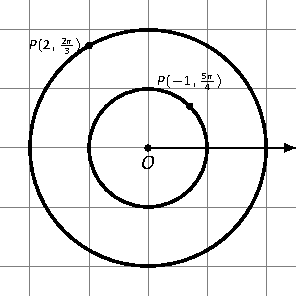
\includegraphics{figures/figpolar2}\\[5pt]
(a)\\[20pt]
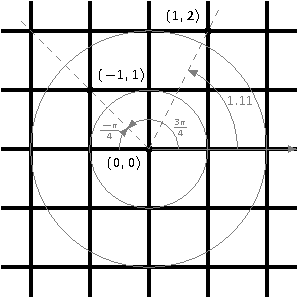
\includegraphics{figures/figpolar2b}\\[5pt]
(b)
\end{tabular}}	

\noindent\textbf{\large Polar Functions and Polar Graphs}\\

Defining a new coordinate system allows us to create a new kind of function, a \textbf{polar function.} Rectangular coordinates lent themselves well to creating functions that related $x$ and $y$, such as $y=x^2.$ Polar coordinates allow us to create functions that relate $r$ and $\theta$. Normally these functions look like $r=f(\theta)$, although we can create functions of the form $\theta = f(r)$. The following examples introduce us to this concept.\index{polar!functions}\index{polar!functions!graphing}\\

\example{ex_polar3}{Introduction to Graphing Polar Functions}{
Describe the graphs of the following polar functions.
\begin{enumerate}
	\item $r = 1.5$
	\item $\theta = \pi/4 $
\end{enumerate}
%
%\noindent$1.\ r = 1.5 \qquad 2.\ \theta = \pi/4 $
}
{\begin{enumerate}
\item The equation $r=1.5$ describes all points that are 1.5 units from the pole; as the angle is not specified, any $\theta$ is allowable. All points 1.5 units from the pole describes a circle of radius 1.5.

\mfigure{.25}{Plotting standard polar plots.}{fig:polar3}{figures/figpolar3}

We can consider the rectangular equivalent of this equation; using $r^2=x^2+y^2$, we see that $1.5^2=x^2+y^2$, which we recognize as the equation of a circle centered at $(0,0)$ with radius 1.5. This is sketched in Figure \ref{fig:polar3}.

\item The equation $\theta = \pi/4$ describes all points such that the line through them and the pole make an angle of $\pi/4$ with the initial ray. As the radius $r$ is not specified, it can be any value (even negative). Thus $\theta = \pi/4$ describes the line through the pole that makes an angle of $\pi/4 = 45^\circ$ with the initial ray: see Figure \ref{fig:polar3}.

We can again consider the rectangular equivalent of this equation. Combine $\tan \theta =y/x$ and $\theta =\pi/4$:
$$\tan \pi/4 = y/x \quad \Rightarrow x\tan \pi/4 = y \quad \Rightarrow y = x.$$ 
\end{enumerate}
\vskip-1.5\baselineskip
}\clearpage

The basic rectangular equations of the form $x=h$ and $y=k$ create vertical and horizontal lines, respectively; the basic polar equations $r= h$ and $\theta =\alpha$ create circles and lines through the pole, respectively. With this as a foundation, we can create more complicated polar functions of the form $r=f(\theta)$. The input is an angle; the output is a length, how far in the direction of the angle to go out.

We sketch these functions much like we sketch rectangular and parametric functions: we plot lots of points and ``connect the dots'' with curves. We demonstrate this in the following example.\\


\example{ex_polar4}{Sketching Polar Functions}{ 
Sketch the polar function $r=1+\cos \theta$ on $[0,2\pi]$ by plotting points.}
{A common question when sketching curves by plotting points is ``Which points should I plot?'' With rectangular equations, we often choose ``easy'' values -- integers, then added more if needed. When plotting polar equations, start with the ``common'' angles -- multiples of $\pi/6$ and $\pi/4$. Figure \ref{fig:polar4} gives a table of just a few values of $\theta$ in $[0,\pi]$. 

\mtable{.6}{Graphing a polar function in\\ Example \ref{ex_polar4} by plotting points.}{fig:polar4}{%
\begin{tabular}{c}
		$\begin{array}{cc}
		\theta & r=1+\cos\theta \\ \hline
 0 & 2 \\
 \pi/6 & 1.86603 \\
  \pi/2 & 1 \\
 4\pi/3 & 0.5 \\
 7 \pi /4 & 1.70711 \\
 \end{array}$\\
 \myincludegraphics[scale=0.9]{figures/figpolar4}
\end{tabular}}

Consider the point $P(0,2)$ determined by the first line of the table. The angle is 0 radians -- we do not rotate from the initial ray -- then we go out 2 units from the pole. When $\theta=\pi/6$, $r = 1.866$ (actually, it is $1+\sqrt{3}/2$); so rotate by $\pi/6$ radians and go out 1.866 units. 

The graph shown uses more points, connected with straight lines. (The points on the graph that correspond to points in the table are signified with larger dots.) Such a sketch is likely good enough to give one an idea of what the graph looks like.
}\\

\noindent\textbf{Technology Note:} Plotting functions in this way can be tedious, just as it was with rectangular functions. To obtain very accurate graphs, technology is a great aid. Most graphing calculators can plot polar functions; in the menu, set the plotting mode to something like \texttt{polar} or \texttt{POL}, depending on one's calculator. As with plotting parametric functions, the viewing ``window'' no longer determines the $x$-values that are plotted, so additional information needs to be provided. Often with the ``window'' settings are the settings for  the beginning and ending $\theta$ values (often called \texttt{$\theta_{\text{min}}$} and \texttt{$\theta_{\text{max}}$}) as well as the \texttt{$\theta_{\text{step}}$} -- that is, how far apart the $\theta$ values are spaced. The smaller the \texttt{$\theta_{\text{step}}$} value, the more accurate the graph (which also increases plotting time). Using technology, we graphed the polar function $r=1+\cos \theta$ from Example \ref{ex_polar4} in Figure \ref{fig:polar4b}.

\mfigure{.3}{Using  technology to graph a polar \\ function.}{fig:polar4b}{figures/figpolar4b}

\example{ex_polar5}{Sketching Polar Functions}{
Sketch the polar function $r=\cos (2\theta)$ on $[0,2\pi]$ by plotting points.}
{We start by making a table of $\cos (2\theta)$ evaluated at common angles $\theta$, as shown in Figure \ref{fig:polar5table}. These points are then plotted in Figure \ref{fig:polar5} (a). This particular graph ``moves'' around quite a bit and one can easily forget which points should be connected to each other. To help us with this, we numbered each point in the table and on the graph. 
%\clearpage

\begin{center}
\begin{minipage}[t]{125pt} \vskip0pt
$\begin{array}{ccc}
\text{Pt.} & \theta & \cos (2\theta)\\ \hline
 1 & 0 & 1. \\
 2 & \pi /6 & 0.5 \\
 3 & \pi /4 & 0. \\
 4 & \pi /3 & -0.5 \\
 5 & \pi /2 & -1. \\
 6 & 2 \pi /3 & -0.5 \\
 7 & 3 \pi /4 & 0. \\
 8 & 5 \pi /6 & 0.5 \\
 9 & \pi  & 1. \\
\end{array}$
\end{minipage}
\begin{minipage}[t]{125pt} \vskip 0pt
$\begin{array}{ccc}
\text{Pt.} & \theta & \cos (2\theta)\\ \hline
 10 & 7 \pi /6 & 0.5 \\
 11 & 5 \pi /4 & 0. \\
 12 & 4 \pi /3 & -0.5 \\
 13 & 3 \pi /2 & -1. \\
 14 & 5 \pi /3 & -0.5 \\
 15 & 7 \pi /4 & 0. \\
 16 & 11 \pi /6 & 0.5 \\
 17 & 2 \pi  & 1. \\
\end{array}$
\end{minipage}
\captionsetup{type=figure}
\caption{Tables of points for plotting a polar curve.}\label{fig:polar5table}
\end{center}
Using more points (and the aid of technology) a smoother plot can be made as shown in Figure \ref{fig:polar5} (b). This plot is an example of a \textit{rose curve}.
\mtable{.65}{Polar plots from Example \ref{ex_polar5}.}{fig:polar5}{%
\begin{tabular}{c}
\myincludegraphics{figures/figpolar5}\\[0pt]
(a) \\[0pt]
\myincludegraphics{figures/figpolar5b}\\[0pt]
(b) 
\end{tabular}
}
}\\

It is sometimes desirable to refer to a graph via a polar equation, and other times by a rectangular equation. Therefore it is necessary to be able to convert between polar and rectangular functions, which we practice in the following example. We will make frequent use of the identities found in Key Idea \ref{idea:polarconvert}.\\

\example{ex_polar6}{Converting between rectangular and polar equations.}{

\noindent
\begin{minipage}[t]{.5\linewidth}
Convert from rectangular to polar.
\begin{enumerate}
	\item $y=x^2$
	\item $xy = 1$
\end{enumerate}
\end{minipage}
\begin{minipage}[t]{.5\linewidth}
Convert from polar to rectangular.
\begin{enumerate}\addtocounter{enumi}{2}
	\item $\ds r=\frac{2}{\sin \theta-\cos\theta}$
	\item $r=2\cos \theta$
\end{enumerate}
\end{minipage}
}
{\begin{enumerate}
	\item Replace $y$ with $r\sin\theta$ and replace $x$ with $r\cos\theta$, giving:
	\begin{align*}
	y &=x^2\\
	r\sin\theta &= r^2\cos^2\theta\\
	\frac{\sin\theta}{\cos^2\theta} &= r
	\end{align*}
	We have found that $r=\sin\theta/\cos^2\theta = \tan\theta\sec\theta$. The domain of this polar function is $(-\pi/2,\pi/2)$; plot a few points to see how the familiar parabola is traced out by the polar equation.
	
	\item		We again replace $x$ and $y$ using the standard identities and work to solve for $r$:
	\begin{align*}
	xy &= 1 \\
	r\cos\theta\cdot r\sin\theta & = 1\\
	r^2 & = \frac{1}{\cos\theta\sin\theta}\\
	r & = \frac{1}{\sqrt{\cos\theta\sin\theta}}\\
	\end{align*}
	This function is valid only when the product of $\cos\theta\sin\theta$ is positive. This occurs in the first and third quadrants, meaning the domain of this polar function is $(0,\pi/2) \cup (\pi,3\pi/2)$.
	
	We can rewrite the original rectangular equation $xy=1$ as $y=1/x$. This is graphed in Figure \ref{fig:polar6}; note how it only exists in the first and third quadrants.
	\mfigure{.25}{Graphing $xy=1$ from Example \ref{ex_polar6}.}{fig:polar6}{figures/figpolar6}
		
	\item		There is no set way to convert from polar to rectangular; in general, we look to form the products $r\cos \theta$ and $r\sin\theta$, and then replace these with $x$ and $y$, respectively. We start in this problem by multiplying both sides by $\sin\theta-\cos\theta$:
	\begin{align*}
	r &= \frac{2}{\sin\theta-\cos\theta} \\
	r(\sin\theta-\cos\theta) &= 2\\
	r\sin\theta-r\cos\theta &= 2. \qquad \text{Now replace with $y$ and $x$:}\\
	y-x &= 2\\
	y &= x+2.
	\end{align*}
	The original polar equation, $r=2/(\sin\theta-\cos\theta)$ does not easily reveal that its graph is simply a line. However, our conversion shows that it is. The upcoming gallery of polar curves gives the general equations of lines in polar form.

\drawexampleline
	
	\item		By multiplying both sides by $r$, we obtain both an $r^2$ term and an $r\cos\theta$ term, which we replace with $x^2+y^2$ and $x$, respectively. 
	\begin{align*}
	r &=2\cos\theta \\
	r^2 &= 2r\cos\theta \\
	x^2+y^2 &= 2x. 
	\intertext{We recognize this as a circle; by completing the square we can find its radius and center.}
	x^2-2x+y^2 &= 0 \\
	(x-1)^2 + y^2 &=1.
	\end{align*}
	The circle is centered at $(1,0)$ and has radius 1. The upcoming gallery of polar curves gives the equations of \textit{some} circles in polar form; circles with arbitrary centers have a complicated polar equation that we do not consider here.
	\end{enumerate}
	\vskip-\baselineskip
}\\

Some curves have very simple polar equations but rather complicated rectangular ones. For instance, the equation $r=1+\cos\theta$ describes a \textit{cardiod} (a shape important the sensitivity of microphones, among other things; one is graphed in the gallery in the Lima\c con section). It's rectangular form is not nearly as simple; it is the implicit equation
$x^4+y^4+2x^2y^2-2xy^2-2x^3-y^2=0.$ The conversion is not ``hard,'' but takes several steps, and is left as a problem in the Exercise section.\\
\pagebreak

\noindent\textbf{\Large Gallery of Polar Curves}\\

There are a number of basic and ``classic'' polar curves, famous for their beauty and/or applicability to the sciences. \index{polar!function!gallery of graphs} This section ends with a small gallery of some of these graphs. We encourage the reader to understand how these graphs are formed, and to investigate with technology other types of polar functions.\\

\enlargethispage{2\baselineskip}
\newlength{\gallerywidth}
\setlength{\gallerywidth}{(0pt+\marginparwidth+\textwidth)/4}
\vskip \baselineskip
\noindent%\hskip-\marginparwidth%\hskip-25pt
\rule{25pt+\marginparwidth+\textwidth}{1pt}\\

\noindent%\hskip-\marginparwidth\hskip-25pt
\textbf{\large Lines}\\

\noindent%\hskip-\marginparwidth\hskip-30pt
\begin{tabular}{p{\gallerywidth}p{\gallerywidth}p{\gallerywidth}p{\gallerywidth}}
\textbf{Through the origin:} & \textbf{Horizontal line:} & \textbf{Vertical line:} & \textbf{Not through origin:} \\[5pt]
$\theta = \alpha$ & $r=a\csc\theta$ & $r=a\sec\theta$ & $\ds r=\frac{b}{\sin\theta-m\cos\theta}$ \\[10pt]
\myincludegraphics[scale=.9]{figures/figpolarline1} & \myincludegraphics[scale=.9]{figures/figpolarline2} & \myincludegraphics[scale=.9]{figures/figpolarline4} & \myincludegraphics[scale=.9]{figures/figpolarline3}
\end{tabular}

%\clearpage\exercisegeometry\exerciseheader
%\ \vskip0pt
%\vskip-.25in
\noindent\parbox{3\gallerywidth+37pt}{\textbf{\large Circles}}\textbf{\large Spiral}\\

\noindent\hskip-5pt%
\begin{tabular}{p{\gallerywidth}p{\gallerywidth}p{\gallerywidth}p{\gallerywidth}}
\textbf{Centered on $x$-axis:} & \textbf{Centered on $y$-axis:} & \textbf{Centered on origin:} &\textbf{Archimedean spiral}\\
$r=a\cos \theta$ & $r=a\sin\theta$ & $r=a$ & $r=\theta$\\
\myincludegraphics[scale=.9]{figures/figpolarcircle1}&\myincludegraphics[scale=.9]{figures/figpolarcircle2}&\myincludegraphics[scale=.9]{figures/figpolarcircle3}&\myincludegraphics[scale=.9]{figures/figpolarspiral}
\end{tabular}\\

\pagebreak

\noindent\hskip-\marginparwidth\hskip-25pt\textbf{\large Lima\c cons}\\

\noindent\hskip-\marginparwidth\hskip-25pt%
\begin{tabular}{p{\gallerywidth}p{\gallerywidth}p{\gallerywidth}p{\gallerywidth}}
\multicolumn{4}{l}{Symmetric about $x$-axis: $r=a\pm b\cos\theta$; \quad Symmetric about $y$-axis:  $r=a\pm b\sin \theta$; \quad $a,b>0$}\\
\\
\textbf{With inner loop:} & \textbf{Cardiod:} & \textbf{Dimpled:} & \textbf{Convex:} \\[5pt]
$\ds \frac ab < 1$ & $\ds \frac ab=1$ & $\ds 1<\frac ab <2$ & $\ds \frac ab>2$ \\[10pt]
\myincludegraphics[scale=.9]{figures/figpolarlimacon1} & \myincludegraphics[scale=.9]{figures/figpolarlimacon2} & \myincludegraphics[scale=.9]{figures/figpolarlimacon3} & \myincludegraphics[scale=.9]{figures/figpolarlimacon4}
\end{tabular}\\

\noindent\hskip-\marginparwidth\hskip-25pt\textbf{\large Rose Curves}\\

\enlargethispage{20\baselineskip}
\noindent\hskip-\marginparwidth\hskip-25pt
\begin{tabular}{p{\gallerywidth}p{\gallerywidth}p{\gallerywidth}p{\gallerywidth}}
\multicolumn{4}{l}{Symmetric about $x$-axis: $r=a \cos(n\theta)$; \quad Symmetric about $y$-axis:  $r=a\sin(n\theta)$}\\
\multicolumn{4}{l}{Curve contains $2n$ petals when $n$ is even and $n$ petals when $n$ is odd.}\\
\\
%\textbf{With inner loop:} & \textbf{Cardiod:} & \textbf{Dimpled:} & \textbf{Convex:} \\[5pt]
$r=a\cos (2\theta)$ & $r=a\sin(2\theta)$ & $r=a\cos (3\theta)$ & $r=a\sin (3\theta)$ \\[10pt]
\myincludegraphics[scale=.9]{figures/figpolarrose1} & \myincludegraphics[scale=.9]{figures/figpolarrose2} & \myincludegraphics[scale=.9]{figures/figpolarrose4} & \myincludegraphics[scale=.9]{figures/figpolarrose3}
\end{tabular}\\
%\clearpage

\noindent\hskip-\marginparwidth\hskip-25pt
\textbf{\large Special Curves}\\

\noindent\hskip-5pt\hskip-\marginparwidth\hskip-25pt%
\begin{tabular}{p{\gallerywidth}p{\gallerywidth}p{\gallerywidth}p{\gallerywidth}}
\textbf{Rose curves} &  & \textbf{Lemniscate:} & \textbf{Eight Curve:} \\[5pt]
$r=a\sin (\theta/5)$ & $r=a\sin(2\theta/5)$ & $r^2=a^2\cos (2\theta)$ & $r^2=a^2\sec^4\theta\cos (2\theta)$ \\[10pt]
\myincludegraphics[scale=.9]{figures/figpolarspecial1} & \myincludegraphics[scale=.9]{figures/figpolarspecial2} & \myincludegraphics[scale=.9]{figures/figpolarspecial3} & \myincludegraphics[scale=.9]{figures/figpolarspecial4}
\end{tabular}\\

\restoregeometry
\regularheader
\pagebreak
%\clearpage

Earlier we discussed how each point in the plane does not have a unique representation in polar form. This can be a ``good'' thing, as it allows for the beautiful and interesting curves seen in the preceding gallery. However, it can also be a ``bad'' thing, as it can be difficult to determine where two curves intersect.\\

\example{ex_polar7}{Finding points of intersection with polar curves}{
Determine where the graphs of the polar equations $r=1+3\cos\theta$ and $r=\cos \theta$ intersect.
}
{As technology is generally readily available, it is usually a good idea to start with a graph. We have graphed the two functions in Figure \ref{fig:polar7}(a); to better discern the intersection points, part (b) of the figure zooms in around the origin.
\mtable{.5}{Graphs to help determine the points of intersection of the polar functions given in Example \ref{ex_polar7}.}{fig:polar7}{%
\begin{tabular}{c}
\myincludegraphics{figures/figpolar7}\\
(a)\\[10pt]
\myincludegraphics{figures/figpolar7b}\\
(b)
\end{tabular}
}
We start by setting the two functions equal to each other and solving for $\theta$:
\begin{align*}
1+3\cos\theta &= \cos \theta \\
2\cos\theta &= -1\\
\cos\theta&= -\frac12\\
\theta &= \frac{2\pi}{3}, \frac{4\pi}{3}.
\end{align*}
(There are, of course, infinite solutions to the equation $\cos\theta=-1/2$; as the lima\c con is traced out once on $[0,2\pi]$, we restrict our solutions to this interval.) 

We need to analyze this solution. When $\theta = 2\pi/3$ we obtain the point of intersection that lies in the 4$^\text{th}$ quadrant. When $\theta = 4\pi/3$, we get the point of intersection that lies in the 2$^\text{nd}$ quadrant. There is more to say about this second intersection point, however. The circle defined by $r=\cos\theta$ is traced out once on $[0,\pi]$, meaning that this point of intersection occurs while tracing out the circle a second time. It seems strange to pass by the point once and then recognize it as a point of intersection only when arriving there a ``second time.'' The first time the circle arrives at this point is when $\theta = \pi/3$.
It is key to understand that these two points are the same: $(\cos \pi/3,\pi/3)$ and $(\cos 4\pi/3,4\pi/3)$. 

To summarize what we have done so far, we have found two points of intersection: when $\theta=2\pi/3$ and when $\theta=4\pi/3$. When referencing the circle $r=\cos \theta$, the latter point is better referenced as when $\theta=\pi/3$.

There is yet another point of intersection: the pole (or, the origin). We did not recognize this intersection point using our work above as each graph arrives at the pole at a different $\theta$ value.

A graph intersects the pole when $r=0$. Considering the circle $r=\cos\theta$, $r=0$ when $\theta = \pi/2$ (and odd multiples thereof, as the circle is repeatedly traced). The lima\c con intersects the pole when $1+3\cos\theta =0$; this occurs when $\cos \theta = -1/3$, or for $\theta = \cos^{-1}(-1/3)$. This is a nonstandard angle, approximately $\theta = 1.9106 = 109.47^\circ$. The lima\c con intersects the pole twice in $[0,2\pi]$; the other angle at which the lima\c con is at the pole is the reflection of the first angle across the $x$-axis. That is, $\theta = 4.3726 = 250.53^\circ.$
}\\

If all one is concerned with is the $(x,y)$ coordinates at which the graphs intersect, much of the above work is extraneous. We know they intersect at $(0,0)$; we might not care at what $\theta$ value. Likewise, using $\theta =2\pi/3$ and $\theta=4\pi/3$ can give us the needed rectangular coordinates. However, in the next section we apply calculus concepts to polar functions. When computing the area of a region bounded by polar curves, understanding the nuances of the points of intersection becomes important.

\printexercises{exercises/09_04_exercises}

\section{Calculus and Polar Functions} \label{sec:polarcalc}
The previous section defined polar coordinates, leading to polar functions. We investigated plotting these functions and solving a fundamental question about their graphs, namely, where do two polar graphs intersect?

We now turn our attention to answering other questions, whose solutions require the use of calculus. A basis for much of what is done in this section is the ability to turn a polar function $r=f(\theta)$ into a set of parametric equations. Using the identities $x=r\cos \theta$ and $y=r\sin \theta$, we can create the parametric equations $x=f(\theta)\cos\theta$, $y=f(\theta)\sin\theta$ and apply the concepts of Section \ref{sec:par_calc}.\\

\noindent\textbf{\large Polar Functions and $\ds \frac{dy}{dx}$}\\

We are interested in the lines tangent a given graph, regardless of whether that graph is produced by rectangular, parametric, or polar equations. In each of these contexts, the slope of the tangent line is $\frac{dy}{dx}$. Given $r=f(\theta)$, we are generally \textit{not} concerned with $r\,'=\fp(\theta)$; that describes how fast $r$ changes with respect to $\theta$. Instead, we will use $x=f(\theta)\cos\theta$, $y=f(\theta)\sin\theta$ to compute $\frac{dy}{dx}$. 

Using Key Idea \ref{idea:dydxpar} we have $$\frac{dy}{dx} = \frac{dy}{d\theta}\Big/\frac{dx}{d\theta}.$$ Each of the two derivatives on the right hand side of the equality requires the use of the Product Rule. We state the important result as a Key Idea.\\

\keyidea{idea:dydxpol}{Finding $\frac{dy}{dx}$ with Polar Functions}
{Let $r=f(\theta)$ be a polar function. With $x=f(\theta)\cos\theta$ and $y=f(\theta)\sin\theta$,
\index{polar!functions!finding $\frac{dy}{dx}$}\index{tangent line}
$$\frac{dy}{dx} = \frac{\fp(\theta)\sin\theta+f(\theta)\cos\theta}{\fp(\theta)\cos\theta-f(\theta)\sin\theta}.$$
}

\example{ex_polcalc1}{Finding $\frac{dy}{dx}$ with polar functions.}
{Consider the lima\c con $r=1+2\sin\theta$ on $[0,2\pi]$.
\begin{enumerate}
	\item Find the equations of the tangent and normal lines to the graph at $\theta=\pi/4$.
	\item		Find where the graph has vertical and horizontal tangent lines.
\end{enumerate}
}
{\begin{enumerate}
	\item We start by computing $\frac{dy}{dx}$. With $\fp(\theta) = 2\cos\theta$, we have
	\begin{align*}
	\frac{dy}{dx} &= \frac{2\cos\theta\sin\theta + \cos\theta(1+2\sin\theta)}{2\cos^2\theta-\sin\theta(1+2\sin\theta)}\\
	&= \frac{\cos\theta(4\sin\theta+1)}{2(\cos^2\theta-\sin^2\theta)-\sin\theta}.
	\end{align*}
	When $\theta=\pi/4$, $\frac{dy}{dx}=-2\sqrt{2}-1$ (this requires a bit of simplification). In rectangular coordinates, the point on the graph at $\theta=\pi/4$ is $(1+\sqrt{2}/2,1+\sqrt{2}/2)$. Thus the rectangular equation of the line tangent to the lima\c con at $\theta=\pi/4$ is 
	$$y=(-2\sqrt{2}-1)\big(x-(1+\sqrt{2}/2)\big)+1+\sqrt{2}/2 \approx  -3.83 x+8.24.$$ The lima\c con and the tangent line are graphed in Figure \ref{fig:polcalc1}. 
	
	The normal line has the opposite--reciprocal slope as the tangent line, so its equation is 
	$$y \approx \frac{1}{3.83}x+1.26.$$
	\mfigure{.75}{The lima\c con in Example \ref{ex_polcalc1} with its tangent line at $\theta=\pi/4$ and points of vertical and horizontal tangency.}{fig:polcalc1}{figures/figpolcalc1}
	\drawexampleline
	
	\item		To find the horizontal lines of tangency, we find where $\frac{dy}{dx}=0$; thus we find where the numerator of our equation for $\frac{dy}{dx}$ is 0.
	$$\cos\theta(4\sin\theta+1)=0\quad \Rightarrow \quad \cos\theta=0 \quad \text{or}\quad 4\sin\theta+1=0.$$
	On $[0,2\pi]$, $\cos\theta=0$ when $\theta=\pi/2,\ 3\pi/2$. 

Setting $4\sin\theta+1=0$ gives $\theta=\sin^{-1}(-1/4)\approx -0.2527 = -14.48^\circ$. We want the results in $[0,2\pi]$; we also recognize there are two solutions, one in the 3$^\text{rd}$ quadrant and one in the 4$^\text{th}$. Using reference angles, we have our two solutions as $\theta =3.39$ and $6.03$ radians. The four points we obtained where the lima\c con has a horizontal tangent line are given in Figure \ref{fig:polcalc1} with black--filled dots.\\

To find the vertical lines of tangency, we set the denominator of $\frac{dy}{dx}=0$. 
\begin{align*}
2(\cos^2\theta -\sin^2\theta)-\sin\theta &= 0 .
\intertext{Convert the $\cos^2\theta$ term to $1-\sin^2\theta$:}
2(1-\sin^2\theta-\sin^2\theta)-\sin\theta &= 0\\
4\sin^2\theta + \sin\theta -1 &= 0.
\intertext{Recognize this as a quadratic in the variable $\sin\theta$. Using the quadratic formula, we have}
\sin\theta &= \frac{-1\pm\sqrt{33}}{8}.
\end{align*}
We solve $\sin\theta = \frac{-1+\sqrt{33}}8$ and $\sin\theta = \frac{-1-\sqrt{33}}8$:
\begin{align*}
\sin\theta &=\frac{-1+\sqrt{33}}8 & \sin\theta &= \frac{-1-\sqrt{33}}{8}\\
\theta &= \sin^{-1}\left(\frac{-1+\sqrt{33}}8\right) & \theta &= \sin^{-1}\left(\frac{-1-\sqrt{33}}8\right)\\
\theta &= 0.6399 & \theta &= -1.0030
\end{align*}
In each of the solutions above, we only get one of the possible two solutions as $\sin^{-1}x$ only returns solutions in $[-\pi/2,\pi/2]$, the 4$^\text{th}$ and $1^\text{st}$ quadrants. Again using reference angles, we have:
$$\sin\theta = \frac{-1+\sqrt{33}}8 \quad \Rightarrow \quad \theta = 0.6399,\ 3.7815 \text{ radians}$$
and 
$$\sin\theta = \frac{-1-\sqrt{33}}8 \quad \Rightarrow \quad \theta = 4.1446,\ 5.2802 \text{ radians.}$$
These points are also shown in Figure \ref{fig:polcalc1} with white--filled dots.
	\end{enumerate}
	\vskip-\baselineskip
}\\

When the graph of the polar function $r=f(\theta)$ intersects the pole, it means that $f(\alpha)=0$ for some angle $\alpha$. Thus the formula for $\frac{dy}{dx}$ in such instances is very simple, reducing simply to $$\frac{dy}{dx} = \tan \alpha.$$
This equation makes an interesting point. It tells us the slope of the tangent line at the pole is $\tan \alpha$; some of our previous work (see, for instance, Example \ref{ex_polar3}) shows us that the line through the pole with slope $\tan \alpha$ has polar equation $\theta=\alpha$. Thus when a polar graph touches the pole at $\theta=\alpha$, the equation of the tangent line at the pole is $\theta=\alpha$. \\

\example{ex_polcalc2}{Finding tangent lines at the pole.}{
Let $r=1+2\sin\theta$, a lima\c con. Find the equations of the lines tangent to the graph at the pole.
\mfigure{.55}{Graphing the tangent lines at the pole in Example \ref{ex_polcalc2}.}{fig:polcalc2}{figures/figpolcalc2}}
{We need to know when $r=0$. 
\begin{align*}
1+2\sin\theta &= 0\\
\sin\theta &= -1/2\\
\theta &= \frac{7\pi}{6},\ \frac{11\pi}6.
\end{align*}
Thus the equations of the tangent lines, in polar, are $\theta = 7\pi/6$ and $\theta = 11\pi/6$. In rectangular form, the tangent lines are $y=\tan(7\pi/6)x$ and $y=\tan(11\pi/6)x$. The full lima\c con can be seen in Figure \ref{fig:polcalc1}; we zoom in on the tangent lines in Figure \ref{fig:polcalc2}.
}\\

\noindent\textbf{\large Area}\\

When using rectangular coordinates, the equations $x=h$ and $y=k$ defined vertical and horzontal lines, respectively, and combinations of these lines create rectangles (hence the name ``rectangular coordinates''). It is then somewhat natural to use rectangles to approximate area as we did when learning about the definite integral.\index{polar!functions!area}

When using polar coordinates, the equations $\theta=\alpha$ and $r=c$ form lines through the origin and circles centered at the origin, respectively, and combinations of these curves form sectors of circles. It is then somewhat natural to calculate the area of regions defined by polar functions by first approximating with sectors of circles. 

Consider Figure \ref{fig:polararea} (a) where a region defined by $r=f(\theta)$ on $[\alpha,\beta]$ is given. (Note how the ``sides'' of the region are the lines $\theta=\alpha$ and $\theta=\beta$, whereas in rectangular coordinates the ``sides'' of regions were often the vertical lines $x=a$ and $x=b$.)
\mnote{.3}{\textbf{Note:} Recall that the area of a sector of a circle with radius $r$ subtended by an angle $\theta$ is $A = \frac12\theta r^2$.

\hfill
\begin{tikzpicture}[x=30pt,y=30pt,thick]
			\draw (2,0) arc (0:50:2) -- (0,0);
			\draw [] (0,0) -- (2,0) node [pos=.5,below] {$r$};
			\draw [fill=black] (0,0) circle (1pt);
			%\draw (1.95,1.0) node {$s$};
			\draw (0,0) node [shift={(15pt,8pt)}] {$\theta$};
			\end{tikzpicture}
\hfill\null
}

Partition the interval $[\alpha,\beta]$ into $n$ equally spaced subintervals as $\alpha = \theta_1 < \theta_2 <\cdots <\theta_{n+1}=\beta$. The length of each subinterval is $\Delta\theta = (\beta-\alpha)/n$, representing a small change in angle. The area of the region defined by the $i\,^\text{th}$ subinterval $[\theta_i,\theta_{i+1}]$ can be approximated with a sector of a circle with radius $f(c_i)$, for some $c_i$ in $[\theta_i,\theta_{i+1}]$. The area of this sector is $\frac12f(c_i)^2\Delta\theta$. This is shown in part (b) of the figure, where $[\alpha,\beta]$ has been divided into 4 subintervals. We approximate the area of the whole region by summing the areas of all sectors:
$$\text{Area} \approx \sum_{i=1}^n \frac12f(c_i)^2\Delta\theta.$$
This is a Riemann sum. By taking the limit of the sum as $n\to\infty$, we find the exact area of the region in the form of a definite integral.
\mtable{.7}{Computing the area of a polar region.}{fig:polararea}{%
\begin{tabular}{c}
\myincludegraphics{figures/figpolarea1}\\
(a)\\[10pt]
\myincludegraphics{figures/figpolarea2}\\
(b)
\end{tabular}
}
\enlargethispage{2\baselineskip}
%\clearpage

\theorem{thm:polar_area}{Area of a Polar Region}
{Let $f$ be continuous and non-negative on $[\alpha,\beta]$, where $0\leq \beta-\alpha\leq 2\pi$. The area  $A$ of the region bounded by the curve $r=f(\theta)$ and the lines $\theta=\alpha$ and $\theta=\beta$ is 
$$
A \ =\  \frac12\int_\alpha^\beta f(\theta)^2 \ d\theta\  =\  \frac12\int_\alpha^\beta r^{\,2} \ d\theta$$
}

The theorem states that $0\leq \beta-\alpha\leq 2\pi$. This ensures that region does not overlap itself, which would give a result that does not correspond directly to the area.\\

%\pagebreak

\example{ex_polcalc3}{Area of a polar region}{
Find the area of the circle defined by $r=\cos \theta$. (Recall this circle has radius $1/2$.)}
{This is a direct application of Theorem \ref{thm:polar_area}. The circle is traced out on $[0,\pi]$, leading to the integral
\begin{align*}
\text{Area} &= \frac12\int_0^\pi \cos^2\theta\ d  \theta \\
						&= \frac12\int_0^\pi \frac{1+\cos(2\theta)}{2}\ d\theta\\
						&= \frac14\big(\theta +\frac12\sin(2\theta)\big)\Bigg|_0^\pi\\
						&= \frac14\pi.
\end{align*}
Of course, we already knew the area of a circle with radius $1/2$. We did this example to demonstrate that the area formula is correct.
}\\

\mnote{.3}{\textbf{Note:} Example \ref{ex_polcalc3} requires the use of the integral $\ds\int \cos^2\theta\ d\theta$. This is handled well by using the power reducing formula as found in the back of this text. Due to the nature of the area formula, integrating $\cos^2\theta$ and $\sin^2\theta$ is required often. We offer here these indefinite integrals as a time--saving measure.\\
$$\int\cos^2\theta\ d\theta = \frac12\theta+\frac14\sin(2\theta)+C$$
$$\int\sin^2\theta\ d\theta = \frac12\theta-\frac14\sin(2\theta)+C$$
}
\pagebreak

\example{ex_polcalc4}{Area of a polar region}{
Find the area of the cardiod $r=1+\cos\theta$ bound between $\theta=\pi/6$ and $\theta=\pi/3$, as shown in Figure \ref{fig:polcalc4}.
}
{This is again a direct application of Theorem \ref{thm:polar_area}. 
\begin{align*}
\text{Area} &= \frac12\int_{\pi/6}^{\pi/3} (1+\cos\theta)^2\ d\theta\\
				&= \frac12\int_{\pi/6}^{\pi/3} (1+2\cos\theta+\cos^2\theta)\ d\theta\\
				&= \frac12\left(\theta+2\sin\theta+\frac12\theta+\frac14\sin(2\theta)\right)\Bigg|_{\pi/6}^{\pi/3} \\
				&= \frac18\big(\pi+4\sqrt{3}-4\big) \approx 0.7587.
				\end{align*}
\vskip-\baselineskip
}\\

\mfigure{.8}{Finding the area of the shaded region of a cardiod in Example \ref{ex_polcalc4}.}{fig:polcalc4}{figures/figpolcalc4}

\noindent\textbf{Area Between Curves}\\

Our study of area in the context of rectangular functions led naturally to finding area bounded between curves. We consider the same in the context of polar functions. \index{polar!functions!area between curves}

Consider the shaded region shown in Figure \ref{fig:polarea3}. We can find the area of this region by computing the area bounded by $r_2=f_2(\theta)$ and subtracting the area bounded by $r_1=f_1(\theta)$ on $[\alpha,\beta]$. Thus
$$\text{Area}\ = \ \frac12\int_\alpha^\beta r_2^{\,2}\ d\theta - \frac12\int_\alpha^\beta r_1^{\,2}\ d\theta = \frac12\int_\alpha^\beta \big(r_2^{\,2}-r_1^{\,2}\big)\ d\theta.$$
\mfigure{.5}{Illustrating area bound between two polar curves.}{fig:polarea3}{figures/figpolarea3}

\keyidea{idea:area_between_polar}{Area Between Polar Curves}
{The area $A$ of the region bounded by $r_1=f_1(\theta)$ and $r_2=f_2(\theta)$, $\theta=\alpha$ and $\theta=\beta$, where $f_1(\theta)\leq f_2(\theta)$ on $[\alpha,\beta]$, is
$$A = \frac12\int_\alpha^\beta \big(r_2^{\,2}-r_1^{\,2}\big)\ d\theta.$$
}

\enlargethispage{2\baselineskip}
\example{ex_polcalc5}{Area between polar curves}{
Find the area bounded between the curves $r=1+\cos \theta$ and $r=3\cos\theta$, as shown in Figure \ref{fig:polcalc5}.
\mfigure{.25}{Finding the area between polar curves in Example \ref{ex_polcalc5}.}{fig:polcalc5}{figures/figpolcalc5}
}
{We need to find the points of intersection between these two functions. Setting them equal to each other, we find:
\begin{align*}
1+\cos\theta &= 3\cos \theta \\
 \cos\theta &=1/2\\
\theta &= \pm \pi/3
\end{align*}
Thus we integrate $\frac12\big((3\cos\theta)^2-(1+\cos\theta)^2\big)$ on $[-\pi/3,\pi/3]$.
\begin{align*}
\text{Area} &= \frac12\int_{-\pi/3}^{\pi/3} \big((3\cos\theta)^2-(1+\cos\theta)^2\big)\ d\theta\\
		&= \frac12\int_{-\pi/3}^{\pi/3} \big( 8\cos^2\theta-2\cos\theta-1\big)\ d\theta \\
		&= \big(2\sin(2\theta) - 2\sin\theta+3\theta\big)\Bigg|_{-\pi/3}^{\pi/3}\\
		&= 2\pi.
\end{align*}
Amazingly enough, the area between these curves has a ``nice'' value.
}\\

\example{ex_polcalc6}{Area defined by polar curves}{
Find the area bounded between the polar curves $r=1$ and $r=2\cos(2\theta)$, as shown in Figure \ref{fig:polcalc6} (a).}
{We need to find the point of intersection between the two curves. Setting the two functions equal to each other, we have
$$2\cos(2\theta) = 1 \quad \Rightarrow \quad \cos(2\theta) = \frac12 \quad \Rightarrow \quad 2\theta = \pi/3\quad \Rightarrow \quad \theta=\pi/6.$$
\mtable{.6}{Graphing the region bounded by the functions in Example \ref{ex_polcalc6}.}{fig:polcalc6}{%
\begin{tabular}{c}
\myincludegraphics{figures/figpolcalc6}\\
(a)\\[10pt]
\myincludegraphics{figures/figpolcalc6a}\\
(b)\\
\end{tabular}
}
In part (b) of the figure, we zoom in on the region and note that it is not really bounded \textit{between} two polar curves, but rather \textit{by} two polar curves, along with $\theta=0$. The dashed line breaks the region into its component parts. Below the dashed line, the region is defined by $r=1$, $\theta=0$ and $\theta = \pi/6$. (Note: the dashed line lies on the line $\theta=\pi/6$.) Above the dashed line the region is bounded by $r=2\cos(2\theta)$ and $\theta =\pi/6$. Since we have two separate regions, we find the area using two separate integrals.

Call the area below the dashed line $A_1$ and the area above the dashed line $A_2$. They are determined by the following integrals:
$$A_1 = \frac12\int_0^{\pi/6} (1)^2\ d\theta\qquad  A_2 = \frac12\int_{\pi/6}^{\pi/4} \big(2\cos(2\theta)\big)^2\ d\theta.$$
(The upper bound of the integral computing $A_2$ is $\pi/4$ as $r=2\cos(2\theta)$ is at the pole when $\theta=\pi/4$.)

We omit the integration details and let the reader verify that $A_1 = \pi/12$ and $A_2 = \pi/12-\sqrt{3}/8$; the total area is $A = \pi/6-\sqrt{3}/8$.
}\\

\noindent\textbf{\large Arc Length}\\

As we have already considered the arc length of curves defined by rectangular and parametric equations, we now consider it in the context of polar equations. Recall that the arc length $L$ of the graph defined by the parametric equations $x=f(t)$, $y=g(t)$ on $[a,b]$ is
\index{arc length}\index{polar!function!arc length}
\begin{equation}L = \int_a^b \sqrt{\fp(t)^2 + g\primeskip'(t)^2}\ dt = \int_a^b \sqrt{x\primeskip'(t)^2+y\primeskip'(t)^2}\ dt.\label{eq:polar_arclength}\end{equation}

Now consider the polar function $r=f(\theta)$. We again use the identities $x=f(\theta)\cos\theta$ and $y=f(\theta)\sin\theta$ to create parametric equations based on the polar function. We compute $x\primeskip'(\theta)$ and $y\primeskip'(\theta)$ as done before when computing $\frac{dy}{dx}$, then apply Equation \eqref{eq:polar_arclength}.

The expression $x\primeskip'(\theta)^2+y\primeskip'(\theta)^2$ can be simplified a great deal; we leave this as an exercise and state that $$x\primeskip'(\theta)^2+y\primeskip'(\theta)^2 = \fp(\theta)^2+f(\theta)^2.$$ This leads us to the  arc length formula.

\keyidea{idea:polar_arclength}{Arc Length of Polar Curves}
{Let  $r=f(\theta)$ be a polar function with $\fp$ continuous on an open interval $I$ containing $[\alpha,\beta]$, on which the graph traces itself only once. The arc length $L$ of the graph on $[\alpha,\beta]$ is
$$L = \int_\alpha^\beta \sqrt{\fp(\theta)^2+f(\theta)^2}\ d\theta = \int_\alpha^\beta\sqrt{(r\,')^2+ r^2}\ d\theta.$$
}

\example{ex_polcalc7}{Arc length of a lima\c con}{
Find the arc length of the lima\c con $r=1+2\sin t$.}
{With $r=1+2\sin t$, we have $r\,' = 2\cos t$. The lima\c con is traced out once on $[0,2\pi]$, giving us our bounds of integration. Applying Key Idea \ref{idea:polar_arclength}, we have
\begin{align*}
L 	&= \int_0^{2\pi} \sqrt{(2\cos\theta)^2+(1+2\sin\theta)^2}\ d\theta \\
		&=	\int_0^{2\pi} \sqrt{4\cos^2\theta+4\sin^2\theta +4\sin\theta+1}\ d\theta\\
		&=	\int_0^{2\pi} \sqrt{4\sin\theta+5}\ d\theta\\
		&\approx 13.3649.
\end{align*}
\mfigure{.45}{The lima\c con in Example \ref{ex_polcalc7} whose arc length is measured.}{fig:polcalc7}{figures/figpolcalc7}
The final integral cannot be solved in terms of elementary functions, so we resorted to a numerical approximation. (Simpson's Rule, with $n=4$, approximates the value with $13.0608$. Using $n=22$ gives the value above, which is accurate to 4 places after the decimal.) 
}\\
\pagebreak

\noindent\textbf{\large Surface Area}\\

The formula for arc length leads us to a formula for surface area. The following Key Idea is based on Key Idea \ref{idea:surface_area_parametric}.

\keyidea{idea:surface_area_polar}{Surface Area of a Solid of Revolution}
{Consider the graph of the polar equation $r=f(\theta)$, where $\fp$ is continuous on an open interval containing $[\alpha,\beta]$ on which the graph does not cross itself.
\index{surface area!solid of revolution}\index{polar!function!surface area}\index{integration!surface area}
	\begin{enumerate}
		\item The surface area of the solid formed by revolving the graph about the initial ray ($\theta=0$) is:
		$$\text{Surface Area} = 2\pi\int_\alpha^\beta f(\theta)\sin\theta\sqrt{\fp(\theta)^2+f(\theta)^2}\ d\theta.$$
		\item The surface area of the solid formed by revolving the graph about the line $\theta=\pi/2$ is:
		$$\text{Surface Area} = 2\pi\int_\alpha^\beta f(\theta)\cos\theta\sqrt{\fp(\theta)^2+f(\theta)^2}\ d\theta.$$
	\end{enumerate}
}
%\clearpage

\example{ex_polcalc8}{Surface area determined by a polar curve}{
Find the surface area formed by revolving one petal of the rose curve $r=\cos(2\theta)$ about its central axis (see Figure \ref{fig:polcalc8}).}
{\mtable{.4}{Finding the surface area of a rose--curve petal that is revolved around its central axis.}{fig:polcalc8}{%
\begin{tabular}{c}
\myincludegraphics{figures/figpolcalc8}\\
(a)\\[10pt]
%%\ifthenelse{\boolean{in_threeD}}{{%
%%\myincludegraphicsthree[width=150pt,3Dmenu,activate=onclick,deactivate=pageinvisible,
%%3Droll=0,
%%3Dortho=0.009,
%%3Dc2c=0.41893383860588074 -0.887881875038147 0.1901581883430481,
%%3Dcoo=65.85308837890625 6.341495513916016 17.98039436340332,
%%3Droo=85,
%%3Dlights=Headlamp,add3Djscript=asylabels.js]{figures/figpolcalc8a_3D}}}%
%%{\myincludegraphics[scale=1.25,trim=5mm 5mm 5mm 5mm,clip=true]{figures/figpolcalc8a}}\\
%%%\myincludegraphicsthree{width=150pt,3Dmenu,activate=onclick,deactivate=pageinvisible,
%%%3Droll=0,
%%%3Dortho=0.009,
%%%3Dc2c=0.41893383860588074 -0.887881875038147 0.1901581883430481,
%%%3Dcoo=65.85308837890625 6.341495513916016 17.98039436340332,
%%%3Droo=85,
%%%3Dlights=Headlamp,add3Djscript=asylabels.js}{scale=1.25,trim=5mm 5mm 5mm 5mm,clip=true}{figures/figpolcalc8a}\\
%%\myincludegraphics[scale=1.25,trim=5mm 5mm 5mm 5mm,clip=true]{figures/figpolcalc8a}\\
\myincludegraphicsthree{width=150pt,3Dmenu,activate=onclick,deactivate=pageinvisible,
3Droll=0,
3Dortho=0.009,
3Dc2c=0.41893383860588074 -0.887881875038147 0.1901581883430481,
3Dcoo=65.85308837890625 6.341495513916016 17.98039436340332,
3Droo=85,
3Dlights=Headlamp,add3Djscript=asylabels.js}{scale=1.25,trim=5mm 5mm 5mm 5mm,clip=true}{figures/figpolcalc8a}\\
(b)\\
\end{tabular}
}
We choose, as implied by the figure, to revolve the portion of the curve that lies on $[0,\pi/4]$ about the initial ray. Using Key Idea \ref{idea:surface_area_polar} and the fact that $\fp(\theta) = -2\sin(2\theta)$, we have
\begin{align*}
\text{Surface Area} &= 2\pi\int_0^{\pi/4} \cos(2\theta)\sin(\theta)\sqrt{\big(-2\sin(2\theta)\big)^2+\big(\cos(2\theta)\big)^2}\ d\theta \\
&\approx 1.36707.
\end{align*}
The integral is another that cannot be evaluated in terms of elementary functions. Simpson's Rule, with $n=4$, approximates the value at $1.36751$.%; with $n=10$, the value is accurate to 4 decimal places.
}\\


This chapter has been about curves in the plane. While there is great mathematics to be discovered in the two dimensions of a plane, we live in a three dimensional world and hence we should also look to do mathematics in 3D -- that is, in \emph{space}. The next chapter begins our exploration into space by introducing the topic of \emph{vectors}, which are incredibly useful and powerful mathematical objects.
\printexercises{exercises/09_05_exercises}

\clearpage{\pagestyle{empty}\cleardoublepage}
\appendix
\thispagestyle{empty}
\clearpage{\pagestyle{empty}\cleardoublepage}

\pagenumbering{arabic}\renewcommand{\thepage}{A.\arabic{page}}
\makeexercisesection{Solutions To Selected Problems}
%
%%
%%
%%%%%
%%%%%%%%%%
%%%%%%%%		 The following makes the index and includes
%%%%%%%%		it in the file
%%%%%%%%%%
%%%%
%%%%\clearpage{\pagestyle{empty}\cleardoublepage}
%%%%\phantomsection
%%%%\addcontentsline{toc}{chapter}{\indexname}
%%%%\printindex
%%%
%%
\qendheader
\eendgeometry
%\cleardoublepage

\phantomsection
\cleardoublepage
\addcontentsline{toc}{chapter}{\indexname}
\printindex
%\includepdf[pages={863-868}]{Calculus.pdf}

%\documentclass[10pt]{book}
%%\usepackage[paperheight=11in,paperwidth=8.5in,%
%%						inner=1in,textheight=7in,textwidth=320pt,marginparwidth=150pt,%
%%						marginparsep=32pt,bottom=3in,footskip=1.5in]{geometry}
%\usepackage[paperheight=11in,paperwidth=8.5in,inner=72pt,%
						%outer=72pt,textheight=10in,%textwidth=320pt,
						%marginparwidth=150pt,%
						%marginparsep=32pt%,%
						%%bottom=3in,footskip=1.5in
						%]{geometry}
												%
%\usepackage{ifthen}
%\usepackage{lipsum}
%\usepackage{tikz}
%\usepackage{amsmath}
%
%\ifthenelse{\boolean{xetex}}%
	%{\sffamily
	%%%\usepackage{fontspec}
	%\usepackage{mathspec}
	%\setallmainfonts[Mapping=tex-text]{Calibri}
	%\setmainfont[Mapping=tex-text]{Calibri}
	%\setsansfont[Mapping=tex-text]{Calibri}
	%\setmathsfont(Greek){[cmmi10]}}
	%{}
\pagestyle{empty}

%\newcommand{\myrule}{\rule[-10pt]{0pt}{15pt}}
%\newcommand{\ds}{\displaystyle}
%\newcommand{\myds}{\ds\myrule}
%\newcommand{\deriv}[2]{\ensuremath{\myds\frac{d}{dx}\left(#1\right)=#2}}
%\newcommand{\myint}[2]{\ensuremath{\myds\int #1\ dx=} \ensuremath{\ds #2}}

%\begin{document}
\noindent\textbf{\large Differentiation Rules}\\
\footnotesize
\noindent\begin{minipage}[t]{.20\linewidth}
\begin{enumerate}
\item \deriv{cx}{c}
\item	\deriv{u\pm v}{u'\pm v'}
\item	\deriv{u\cdot v}{uv'+ u'v}
\item	\deriv{\frac uv}{\frac{vu'-uv'}{v^2}}
\item	\deriv{u(v)}{u'(v)v'}
\item	\deriv{c}{0}
\item	\deriv{x}{1}
\item	\deriv{x^n}{nx^{n-1}}
\item	\deriv{e^x}{e^x}
\end{enumerate}
\end{minipage}
\begin{minipage}[t]{.23\linewidth}
\begin{enumerate}\addtocounter{enumi}{9}
\item	\deriv{a^x}{\ln a\cdot a^x}
\item	\deriv{\ln x}{\frac{1}{x}}
\item	\deriv{\log_a x}{\frac{1}{\ln a}\cdot \frac1x}
\item	\deriv{\sin x}{\cos x}
\item	\deriv{\cos x}{-\sin x}
\item	\deriv{\csc x}{-\csc x\cot x}
\item	\deriv{\sec x}{\sec x\tan x}
\item	\deriv{\tan x}{\sec^2 x}
\item	\deriv{\cot x}{-\csc^2 x}
\end{enumerate}
\end{minipage}
\begin{minipage}[t]{.25\linewidth}
\begin{enumerate}\addtocounter{enumi}{18}
\item	\deriv{\sin^{-1}x}{\frac{1}{\sqrt{1-x^2}}}
\item	\deriv{\cos^{-1}x}{\frac{-1}{\sqrt{1-x^2}}}
\item	\deriv{\csc^{-1}x}{\frac{-1}{x\sqrt{x^2-1}}}
\item	\deriv{\sec^{-1}x}{\frac{1}{x\sqrt{x^2-1}}}
\item	\deriv{\tan^{-1}x}{\frac{1}{1+x^2}}
\item	\deriv{\cot^{-1}x}{\frac{-1}{1+x^2}}
\item	\deriv{\cosh x}{\sinh x}
\item \deriv{\sinh x}{\cosh x}
\item \deriv{\tanh x}{\sech^2 x}
\end{enumerate}
\end{minipage}
\begin{minipage}[t]{.25\linewidth}
\begin{enumerate}\addtocounter{enumi}{27}
\item \deriv{\sech x}{-\sech x\tanh x}
\item	\deriv{\csch x}{-\csch x\coth x}
\item	\deriv{\coth x}{-\csch^2 x}
\item	\deriv{\cosh^{-1}x}{\frac1{\sqrt{x^2-1}}}
\item	\deriv{\sinh^{-1}x}{\frac1{\sqrt{x^2+1}}}
\item	\deriv{\sech^{-1}x}{\frac{-1}{x\sqrt{1-x^2}}}
\item	\deriv{\csch^{-1}x}{\frac{-1}{|x|\sqrt{1+x^2}}}
\item	\deriv{\tanh^{-1}x}{\frac1{1-x^2}}
\item	\deriv{\coth^{-1}x}{\frac1{1-x^2}}
\end{enumerate}
\end{minipage}
\vskip4\baselineskip
\noindent\textbf{\large Integration Rules}\\

\noindent%
\begin{minipage}[t]{.30\linewidth}
\begin{enumerate}
\item	\myint{c\cdot f(x)}{c\int f(x)\ dx}
\item	\myint{f(x)\pm g(x)}{}\\
$\ds \int f(x)\ dx \pm \int g(x)\ dx$
\item	\myint{0}{C}
\item	\myint{1}{x+C}
\item	\myint{x^n}{\frac{1}{n+1}x^{n+1}+C, \ n\neq -1}\\
$\ n\neq -1$
\item	\myint{e^x}{e^x+C}
\item	\myint{a^x}{\frac{1}{\ln a}\cdot a^x+C}
\item	\myint{\frac{1}{x}}{\ln |x| + C}
\item	\myint{\cos x}{\sin x+C}
\item	\myint{\sin x}{-\cos x+C}
\end{enumerate}
\end{minipage}
\begin{minipage}[t]{.31\linewidth}
\begin{enumerate}\addtocounter{enumi}{10}
\item	\myint{\tan x}{-\ln |\cos x|+C}
\item	\myint{\sec x}{\ln |\sec x+\tan x|+C}
\item	\myint{\csc x}{-\ln |\csc x+\cot x|+C}
\item	\myint{\cot x}{\ln |\sin x|+C}
\item	\myint{\sec^2 x}{\tan x+C}
\item	\myint{\csc^2x}{-\cot x+C}
\item	\myint{\sec x\tan x}{\sec x+C}
\item	\myint{\csc x\cot x}{-\csc x+C}
\item	\myint{\cos^2x}{\frac12x+\frac14\sin\big(2x\big)+C}
\item	\myint{\sin^2x}{\frac12x-\frac14\sin\big(2x\big)+C}
\item	\myint{\frac{1}{x^2+a^2}}{\frac1a\tan^{-1}\left(\frac xa\right)+C}
\end{enumerate}
\end{minipage}
\begin{minipage}[t]{.38\linewidth}
\begin{enumerate}\addtocounter{enumi}{21}
\item	\myint{\frac{1}{\sqrt{a^2-x^2}}}{\sin^{-1}\left(\frac xa\right)+C}
\item	\myint{\frac{1}{x\sqrt{x^2-a^2}}}{\frac1a\sec^{-1}\left(\frac{x}{a}\right)+C}
\item	\myint{\cosh x}{\sinh x+C}
\item	\myint{\sinh x}{\cosh x+C}
\item	\myint{\tanh x}{\ln(\cosh x)+C}
\item	\myint{\coth x}{\ln |\sinh  x|+C}
\item	\myint{\frac{1}{\sqrt{x^2-a^2}}}{\ln\big|x+\sqrt{x^2-a^2}\big|+C}
\item	\myint{\frac{1}{\sqrt{x^2+a^2}}}{\ln\big|x+\sqrt{x^2+a^2}\big|+C}
\item	\myint{\frac{1}{a^2-x^2}}{\frac12\ln\left|\frac{a+x}{a-x}\right|+C}
\item	\myint{\frac{1}{x\sqrt{a^2-x^2}}}{\frac1a\ln\left(\frac{x}{a+\sqrt{a^2-x^2}}\right)+C}
\item	\myint{\frac{1}{x\sqrt{x^2+a^2}}}{\frac1a\ln\left|\frac{x}{a+\sqrt{x^2+a^2}}\right|+C}
\end{enumerate}
\end{minipage}
\normalsize

\clearpage

\noindent%
\begin{minipage}[t]{.53\linewidth}
\noindent\textbf{\large The Unit Circle}

\begin{tikzpicture}[scale=3]
\draw [<->,>=latex] (-1.5,0) -- (1.4,0) node [right] {\scriptsize $x$};
\draw [<->,>=latex] (0,-1.3) -- (0,1.3) node [above] {\scriptsize $y$};
\foreach \x / \y / \z / \w / \v in {
								0/0/{1,0}/right/white,
								30/{\pi/6}/{\frac{\sqrt{3}}2,\frac 12}/above right/none,%
								45/{\pi/4}/{\frac{\sqrt{2}}2,\frac{\sqrt{2}}2}/above right/none,
								60/{\pi/3}/{\frac{1}2,\frac{\sqrt{3}}2}/{above right}/none,
								90/ {\pi/2}/{0,1}/above/white,%
								120/{2\pi/3}/{-\frac{1}2,\frac{\sqrt{3}}2}/above left/none, 
								135/{3\pi/4}/{-\frac{\sqrt{2}}2,\frac{\sqrt{2}}2}/above left/none, 
								150/ {5\pi/6}/{-\frac{\sqrt{3}}2,\frac{1}2}/above left/none,%
								180/ {\pi}/{-1,0}/left/white, 
								210/{7\pi/6}/{-\frac{\sqrt{3}}2,-\frac{1}2}/below left/none, 
								225/{5\pi/4}/{-\frac{\sqrt{2}}2,-\frac{\sqrt{2}}2}/below left/none, 
								240/{4\pi/3}/{-\frac{1}2,-\frac{\sqrt{3}}2}/below left/none,
								270/{3\pi/2}/{0,-1}/below/white, 
								300/{5\pi/3}/{\frac{1}2,-\frac{\sqrt{3}}2}/below right/none, 
								315/{7\pi/4}/{\frac{\sqrt{2}}2,-\frac{\sqrt{2}}2}/below right/none, 
								330/{11\pi/6}/{\frac{\sqrt{3}}2,-\frac{1}2}/below right/none%
										}
	{%
		\draw (\x:.65cm) node [fill=\v] {\scriptsize \x$^\circ$};
		\draw (\x:.85cm) node [fill=\v] {\scriptsize $\y$};
		\draw (\x:1cm) node [\w,fill=\v] {\scriptsize $\left(\z\right)$};
		\draw [fill=black] (\x:1) circle (.5pt);
	}

\draw [thick] (0,0) circle (1);

\end{tikzpicture}
\end{minipage}
%
\begin{minipage}[t]{.45\linewidth}
\noindent\textbf{\large Definitions of the Trigonometric Functions}\\

\noindent%
\small
%\begin{minipage}[t]{.48\linewidth}
\textbf{\normalsize Unit Circle Definition}

\noindent
%
\begin{minipage}{.56\linewidth}
\centering
\vskip 0in\begin{tikzpicture}[>=latex,scale=1.5,thick]
\draw [<->](-1.3,0)--(1.3,0) node [right] {$x$};
\draw [<->] (0,-1.3) -- (0,1.3) node [above] {$y$};
\draw (0,0) circle (1);
\draw [fill= black] (-.6,.8) circle (1pt);
\draw (0,0) -- (-.6,.8) node [above left] {$(x,y)$};
\draw [->] (.5,0) arc (0:127:.5);
\draw [dashed,thin] (-.6,.8) -- (-.6,0) node [pos=.5,left] {$y$};
\draw (-.3,0) node [below] {$x$};
\draw (.45,.45) node {$\theta$};
\end{tikzpicture}
\end{minipage}
\begin{minipage}{.4\linewidth}
\vskip 0in \small
\begin{tabular}{cc}
$\sin \theta = y$ & $\cos \theta = x$ \\
\\
$\ds\csc \theta = \frac1y$&$\ds\sec \theta = \frac1x$ \\
\\
$\myrule\ds\tan \theta = \frac yx$ & $\ds\cot \theta = \frac xy$
\end{tabular}
\end{minipage}
%\rule[-50pt]{.5pt}{100pt}
%
%\end{minipage}\hskip .02\linewidth
%\begin{minipage}[t]{.5\linewidth}
%Right Triangle Definition\\
%
%\noindent
\noindent\textbf{\normalsize Right Triangle Definition}

\begin{minipage}{.56\linewidth}
\centering
\begin{tikzpicture}[thick]
\draw (0,0) -- (2.5,0) node [below,pos=.5] {Adjacent} -- (2.5,2) node [pos=.5,rotate=-90,shift={(0pt,7pt)}] {Opposite} -- (0,0) node [pos=.5,above,rotate=38.7] {Hypotenuse} node [shift={(20pt,8pt)}] {$\theta$};
\draw[->,>=latex] (1,0) arc (0:38.7:1);
\draw (2.2,0) -- (2.2,.3) -- (2.5,.3);
\end{tikzpicture}
\end{minipage}
\begin{minipage}{.4\linewidth}
\vskip 0in \small
\begin{tabular}{cc}
$\ds\sin \theta = \frac{\text{O}}{\text{H}}$ & $\ds\csc \theta = \frac{\text{H}}{\text{O}}$ \\
\\
$\ds\cos \theta = \frac{\text{A}}{\text{H}}$ & $\ds\sec \theta = \frac{\text{H}}{\text{A}}$ \\
\\
$\ds\tan \theta = \frac{\text{O}}{\text{A}}$ & $\ds\cot \theta = \frac{\text{A}}{\text{O}}$ \\
\end{tabular}
\end{minipage}
\end{minipage}
\normalsize

\vskip \baselineskip
\noindent\textbf{\large Common Trigonometric Identities}\\
\vskip \baselineskip
\noindent%
\begin{minipage}[t]{.25\linewidth}
	\noindent\textbf{Pythagorean Identities}\vskip 5pt

	\noindent$\ds \sin ^2x+\cos ^2x= 1$\vskip 5pt

	\noindent$\ds \tan^2x+ 1 = \sec^2 x$\vskip 5pt

	\noindent$\ds 1 + \cot^2x=\csc^2 x$\vskip 5pt
\end{minipage}
\begin{minipage}[t]{.45\linewidth}
	\textbf{Cofunction Identities}\vskip 5pt
	\begin{minipage}[t]{.45\linewidth}
		$\ds \sin\left(\frac{\pi}{2}-x\right) = \cos x$\vskip 5pt
		$\ds \cos\left(\frac{\pi}{2}-x\right) = \sin x$\vskip 5pt
		$\ds \tan\left(\frac{\pi}{2}-x\right) = \cot x$\vskip 5pt
	\end{minipage}
	\begin{minipage}[t]{.45\linewidth}
		$\ds \csc\left(\frac{\pi}{2}-x\right) = \sec x$\vskip 5pt
		$\ds \sec\left(\frac{\pi}{2}-x\right) = \csc x$\vskip 5pt
		$\ds \cot\left(\frac{\pi}{2}-x\right) = \tan x$\vskip 5pt
	\end{minipage}
\end{minipage}
\begin{minipage}[t]{.25\linewidth}
	\textbf{Double Angle Formulas}\vskip 5pt
	$\sin 2x = 2\sin x\cos x$ \vskip 5pt
	$\cos 2x = \cos^2x - \sin^2 x$\vskip 5pt
	$\phantom{\cos 2x}= 2\cos^2x-1$\vskip 5pt
	$\phantom{\cos 2x}= 1-2\sin^2x$\vskip 5pt
	$\ds\tan 2x = \frac{2\tan x}{1-\tan^2 x}$
\end{minipage}

\vskip \baselineskip

\noindent%
\begin{minipage}[t]{.44\linewidth}
\textbf{Sum to Product Formulas}\vskip 5pt
$\ds \sin x+\sin y = 2\sin \left(\frac{x+y}2\right)\cos\left(\frac{x-y}2\right)$\vskip 5pt
$\ds \sin x-\sin y = 2\sin \left(\frac{x-y}2\right)\cos\left(\frac{x+y}2\right)$\vskip 5pt
$\ds \cos x+\cos y = 2\cos \left(\frac{x+y}2\right)\cos\left(\frac{x-y}2\right)$\vskip 5pt
$\ds \cos x-\cos y = -2\sin \left(\frac{x+y}2\right)\sin\left(\frac{x-y}2\right)$\vskip 5pt
\end{minipage}
\begin{minipage}[t]{.3\linewidth}
\textbf{Power--Reducing Formulas}\vskip 5pt
$\ds \sin^2 x = \frac{1-\cos 2x}{2}$\vskip 5pt
$\ds \cos^2 x = \frac{1+\cos 2x}{2}$\vskip 5pt
$\ds \tan^2x = \frac{1-\cos 2x}{1+\cos 2x}$
\end{minipage}
\begin{minipage}[t]{.25\linewidth}
\textbf{Even/Odd Identities}\vskip 5pt
$\sin(-x) = -\sin x$\vskip 5pt
$\cos (-x) = \cos x$\vskip 5pt
$\tan (-x) = -\tan x$\vskip 5pt
$\csc(-x) = -\csc x$\vskip 5pt
$\sec (-x) = \sec x$\vskip 5pt
$\cot (-x) = -\cot x$\vskip 5pt
\end{minipage}

\vskip \baselineskip

\noindent
\begin{minipage}[t]{.45\linewidth}
\textbf{Product to Sum Formulas}\vskip 5pt
$\ds \sin x\sin y = \frac12 \big(\cos(x-y) - \cos (x+y)\big)$\vskip 5pt
$\ds \cos x\cos y = \frac12\big(\cos (x-y) +\cos (x+y)\big)$\vskip 5pt
$\ds \sin x\cos y = \frac12 \big(\sin(x+y) + \sin (x-y)\big)$\vskip 5pt
\end{minipage}
\begin{minipage}[t]{.45\linewidth}
\textbf{Angle Sum/Difference Formulas}\vskip 5pt
$\sin (x\pm y) = \sin x\cos y \pm \cos x\sin y$\vskip 5pt
$\cos (x\pm y) = \cos x\cos y \mp \sin x\sin y$\vskip 5pt
$\ds \tan (x\pm y) = \frac{\tan x\pm \tan y}{1\mp \tan x\tan y}$
\end{minipage}

\clearpage

\noindent\textbf{\large Areas and Volumes}
\vskip \baselineskip
%\begin{tabular}{cc}
\noindent%
%
\begin{minipage}[t]{225pt}
		\begin{minipage}[t]{100pt}
		\noindent\textbf{Triangles}\vskip 5pt
		$h=a\sin \theta$\vskip 5pt
		Area = $\frac12bh$\vskip 5pt
		Law of Cosines:%\vskip 4pt
		
		$c^2=a^2+b^2-2ab\cos \theta$\vskip 5pt
		\end{minipage}
		\begin{minipage}[t]{115pt}
			\centering
			\vskip 0pt
			\begin{tikzpicture}[x=30pt,y=30pt,thick]
			\draw (0,0) -- node [below,pos=.5]  { $b$} (3,0) node [shift={(-15pt,8pt)}] {$\theta$} -- node [pos=.5,right] { $a$} (2,1.5) -- node [pos=.5,above left] { $c$} (0,0);
			\draw (2.7,0) arc (180:125:.3);
			\draw [dashed] (2,1.5) -- (2,0) node [pos=.5,left] {$h$};
			\draw (2,.2) -- (1.8,.2) -- (1.8,0);
			\end{tikzpicture}
		\end{minipage}
\end{minipage}
%
\begin{minipage}[t]{225pt}
	\begin{minipage}[t]{100pt}
		\noindent\textbf{Right Circular Cone}\vskip 5pt
		Volume = $\frac 13 \pi r^2h$ \vskip 5pt
		Surface Area =\vskip 3pt		
		 $\pi r\sqrt{r^2+h^2} +\pi r^2$
		\end{minipage}
		\begin{minipage}[t]{115pt}
			\centering
			\vskip 0pt
			\begin{tikzpicture}[x=13pt,y=15pt,thick]
			\begin{scope}[xscale=2]
			\draw (-1,0) arc (-180:0:1);
			\draw [dashed] (1,0) arc (0:180:1);
			\draw (-1,.1) -- (0,3) -- (1,.15);
			\draw [dashed] (0,3) -- node [pos=.5,left] {\small $h$} (0,0);
			\draw [dashed] (0,0) -- (1,0) node [pos=.5,above] {\small $r$};
			\end{scope}
			\draw [fill=black] (0,0) circle (1pt);
			\end{tikzpicture}
		\end{minipage}
\end{minipage}

\vskip 2\baselineskip
\noindent%
\begin{minipage}[t]{225pt}
		\begin{minipage}[t]{100pt}
		\noindent\textbf{Parallelograms}\vskip 5pt
		Area = $bh$
		\end{minipage}
		\begin{minipage}[t]{115pt}
			\centering
			\vskip 0pt
			\begin{tikzpicture}[x=30pt,y=25pt,thick]
			\draw (0,0) -- node [below,pos=.5]  { $b$} (2,0) -- (3,1.5) -- (1,1.5) -- (0,0);
			\draw [dashed] (1,1.5) -- (1,0) node [pos=.5,right] {$h$};
			\draw (.8,0) -- (.8,.2) -- (1,.2);
			\end{tikzpicture}
		\end{minipage}
\end{minipage}
\begin{minipage}[t]{225pt}
\begin{minipage}[t]{100pt}
		\noindent\textbf{Right Circular Cylinder}\vskip 5pt
		Volume = $\pi r^2h$ \vskip 5pt
		Surface Area =\vskip 3pt		
		 $2\pi rh  +2\pi r^2$
		\end{minipage}
		\begin{minipage}[t]{115pt}
			\centering
			\vskip 0pt
			\begin{tikzpicture}[x=13pt,y=14pt,thick]
			\begin{scope}[xscale=2]
			\draw (-1,0) arc (-180:0:1);
			\draw [dashed] (1,0) arc (0:180:1);
			\draw (0,2.5) circle (1);
			\draw (-1,0) -- (-1,2.5) (1,0)-- (1,2.5) node [right,pos=.5] {$h$};
			\draw (0,2.5) -- (1,2.5) node [above,pos=.5] {$r$};
			\end{scope}
			\draw [fill=black] (0,2.5) circle (1pt);
			\end{tikzpicture}
		\end{minipage}

		
\end{minipage}

\vskip 2\baselineskip
\noindent%
\begin{minipage}[t]{225pt}
		\begin{minipage}[t]{100pt}
		\noindent\textbf{Trapezoids}\vskip 5pt
		Area = $\frac12(a+b)h$
		\end{minipage}
		\begin{minipage}[t]{115pt}
			\centering
			\vskip 0pt
			\begin{tikzpicture}[x=30pt,y=25pt,thick]
			\draw (0,0) -- node [below,pos=.7]  { $b$} (3,0) -- (2.5,1.5) -- node [above,pos=.5] {$a$} (1.5,1.5) -- (0,0);
			\draw [dashed] (1.5,1.5) -- (1.5,0) node [pos=.5,right] {$h$};
			\draw (1.3,0) -- (1.3,.2) -- (1.5,.2);
			\end{tikzpicture}
		\end{minipage}
\end{minipage}
\begin{minipage}[t]{225pt}
\begin{minipage}[t]{100pt}
		\noindent\textbf{Sphere}\vskip 5pt
		Volume = $\frac43\pi r^3$ \vskip 5pt
		Surface Area =$4\pi r^2$
		\end{minipage}
		\begin{minipage}[t]{115pt}
			\centering
			\vskip 0pt
			\begin{tikzpicture}[x=13pt,y=13pt,thick]
			\begin{scope}[xscale=2]
			\draw (-1,0) arc (-180:0:1);
			\draw [dashed] (1,0) arc (0:180:1);
			\end{scope}
			\draw (0,0) circle (2);
			\draw [dashed] (0,0) -- (2,0) node [pos=.5,above] {$r$};
			\draw [fill=black] (0,0) circle (1pt);
			\end{tikzpicture}
		\end{minipage}
\end{minipage}

\vskip 2\baselineskip
\noindent%
\begin{minipage}[t]{225pt}
		\begin{minipage}[t]{100pt}
		\noindent\textbf{Circles}\vskip 5pt
		Area = $\pi r^2$\vskip 5pt
		Circumference = $2\pi r$
		\end{minipage}
		\begin{minipage}[t]{115pt}
			\centering
			\vskip 0pt
			\begin{tikzpicture}[x=30pt,y=30pt,thick]
			\draw (0,0) circle (1);
			\draw [dashed] (0,0) -- (1,0) node [pos=.5,above] {$r$};
			\draw [fill=black] (0,0) circle (1pt);
			\end{tikzpicture}
		\end{minipage}
\end{minipage}
\begin{minipage}[t]{225pt}
\begin{minipage}[t]{100pt}
		\noindent\textbf{General Cone}\vskip 5pt
		Area of Base = $A$\vskip 5pt
		Volume = $\frac13Ah$ \vskip 5pt
		\end{minipage}
		\begin{minipage}[t]{115pt}
			\centering
			\vskip 0pt
			\begin{tikzpicture}[x=13pt,y=10pt,thick]
			\begin{scope}
			\clip (0,0) rectangle (4,-2.5);
			\draw [smooth] plot coordinates {(0,0) (1,1.5) (2,1.5) (4,0) (3,-1) (2,-1.5) (1,-2) (0,0)};
			\end{scope}
			\begin{scope}
			\clip (0,0) rectangle (4,2.5);
			\draw [smooth,dashed] plot coordinates {(0,0) (1,1.5) (2,1.5) (4,0) (3,-1) (2,-1.5) (1,-2) (0,0)};
			\end{scope}
			\draw (0,0) -- (2,4)--(4,0);
			\draw [dashed] (2,0)--(2,4) node [pos=.5,right] {$h$}; 
			\draw [fill=black](2,0) circle (1pt);
			\draw (1.5,-.75) node {$A$};
			\end{tikzpicture}
		\end{minipage}
\end{minipage}

\vskip 2\baselineskip
\noindent%
\begin{minipage}[t]{225pt}
		\begin{minipage}[t]{100pt}
		\noindent\textbf{Sectors of Circles}\vskip 5pt
		$\theta$ in radians \vskip 5pt
		Area = $\frac12\theta r^2$\vskip 5pt
		$s=r\theta$
		\end{minipage}
		\begin{minipage}[t]{115pt}
			\centering
			\vskip 0pt
			\begin{tikzpicture}[x=30pt,y=30pt,thick]
			\draw (2,0) arc (0:50:2) -- (0,0);
			\draw [] (0,0) -- (2,0) node [pos=.5,below] {$r$};
			\draw [fill=black] (0,0) circle (1pt);
			\draw (1.95,1.0) node {$s$};
			\draw (0,0) node [shift={(15pt,8pt)}] {$\theta$};
			\end{tikzpicture}
		\end{minipage}
\end{minipage}
\begin{minipage}[t]{225pt}
\begin{minipage}[t]{100pt}
		\noindent\textbf{General Right Cylinder}\vskip 5pt
		Area of Base = $A$\vskip 5pt
		Volume = $Ah$ \vskip 5pt
		\end{minipage}
		\begin{minipage}[t]{115pt}
			\centering
			\vskip 0pt
			\begin{tikzpicture}[x=13pt,y=10pt,thick]
			\begin{scope}
			\clip (0,0) rectangle (4,-2.5);
			\draw [smooth] plot coordinates {(0,0) (1,1.5) (2,1.5) (4,0) (3,-1) (2,-1.5) (1,-2) (0,0)};
			\end{scope}
			\begin{scope}
			\clip (0,0) rectangle (4,2.5);
			\draw [smooth,dashed] plot coordinates {(0,0) (1,1.5) (2,1.5) (4,0) (3,-1) (2,-1.5) (1,-2) (0,0)};
			\end{scope}
			\begin{scope}[shift={(0,4)}]
			\draw [smooth] plot coordinates {(0,0) (1,1.5) (2,1.5) (4,0) (3,-1) (2,-1.5) (1,-2) (0,0)};
			\end{scope}
			\draw (0,0) -- (0,4) (4,0) -- (4,4) node [pos=.5,right] {$h$};
			\draw (2,0) node {$A$};
			\end{tikzpicture}
		\end{minipage}
\end{minipage}

\clearpage

\noindent\textbf{\Large Algebra}\vskip 2\baselineskip

\noindent \textbf{\large Factors and Zeros of Polynomials}\\
Let $p(x) = a_n x^n + a_{n-1} x^{n-1} + \cdots + a_1 x + a_0$ be a polynomial.  If $p(a)=0$, then $a$ is a $zero$ of the polynomial and a solution
of the equation $p(x)=0$.  Furthermore, $(x-a)$ is a $factor$ of the polynomial.
\vskip\baselineskip

\noindent \textbf{\large Fundamental Theorem of Algebra}\\
An $n$th degree polynomial has $n$ (not necessarily distinct) zeros.  Although all of these zeros may be imaginary, a real polynomial of odd degree
must have at least one real zero.\\
\vskip\baselineskip

\noindent \textbf{\large Quadratic Formula}\\
If $p(x) = ax^2 + bx + c$, and $0 \le b^2 - 4ac$, then the real zeros of $p$ are $x=(-b\pm \sqrt{b^2-4ac})/2a$\\
\vskip\baselineskip

\noindent \textbf{\large Special Factors}\\
$
\begin{array}{ll}
x^2 - a^2 = (x-a)(x+a) \qquad \qquad \qquad & x^3 - a^3 = (x-a)(x^2+ax+a^2)\\	
x^3 + a^3 = (x+a)(x^2-ax+a^2) \qquad \qquad \qquad & x^4 - a^4 = (x^2-a^2)(x^2+a^2)\\	
\end{array}
$

\noindent$\begin{array}{l}
(x+y)^n  =x^n + nx^{n-1}y+\frac{n(n-1)}{2!}x^{n-2}y^2+\cdots +nxy^{n-1}+y^n\\
(x-y)^n  =x^n - nx^{n-1}y+\frac{n(n-1)}{2!}x^{n-2}y^2-\cdots \pm nxy^{n-1}\mp y^n
\end{array}$\vskip \baselineskip


\noindent \textbf{\large Binomial Theorem}\\
$
\begin{array}{ll}
(x+y)^2 = x^2 + 2xy + y^2 \qquad & (x-y)^2 = x^2 -2xy +y^2\\
(x+y)^3 = x^3 + 3x^2y + 3xy^2 + y^3 \qquad  & (x-y)^3 = x^3 -3x^2y + 3xy^2 -y^3\\
(x+y)^4 = x^4 + 4x^3y + 6x^2y^2 + 4xy^3 + y^4 \qquad  & (x-y)^4 = x^4 - 4x^3y + 6x^2y^2 - 4xy^3 + y^4\\
\end{array}
$\vskip\baselineskip

\noindent \textbf{\large Rational Zero Theorem}\\
If $p(x) = a_n x^n + a_{n-1} x^{n-1} + \cdots + a_1 x + a_0$ has integer coefficients, then every $rational$ $zero$ of $p$ is of the form
$x=r/s$, where $r$ is a factor of $a_0$ and $s$ is a factor of $a_n$.\\
\vskip\baselineskip

\noindent \textbf{\large Factoring by Grouping}\\
$ac x^3 + adx^2 + bcx + bd = ax^2(cx+d)+b(cx+d)=(ax^2+b)(cx+d)$\\
\vskip\baselineskip

\noindent \textbf{\large Arithmetic Operations}\\
$
\begin{array}{lll}
ab+ac=a(b+c) \qquad \qquad & \displaystyle \frac{a}{b}+\frac{c}{d} = \frac{ad+bc}{bd} \qquad \qquad & \displaystyle \frac{a+b}{c} = \frac{a}{c} + \frac{b}{c}\\	\\
\displaystyle\frac{\left(\displaystyle\frac{a}{b}\right)}{\left(\displaystyle\frac{c}{d}\right)}=\left(\frac{a}{b}\right)\left(\frac{d}{c}\right)=\frac{ad}{bc} 
&\displaystyle \frac{\left(\displaystyle\frac{a}{b}\right)}{c} =\displaystyle \frac{a}{bc}
&\displaystyle \frac{a}{\left(\displaystyle\frac{b}{c}\right)} =\displaystyle \frac{ac}{b}\\ \\
a\left(\displaystyle\frac{b}{c}\right)= \displaystyle \frac{ab}{c}&\displaystyle\frac{a-b}{c-d}=\frac{b-a}{d-c}&\displaystyle\frac{ab+ac}{a}=b+c\\
\end{array}
$\vskip \baselineskip

\noindent \textbf{\large Exponents and Radicals}\\[5pt]
$
\begin{array}{llllll}
a^0=1, \; \; a \ne 0 \quad & (ab)^x=a^xb^x \quad & a^xa^y = a^{x+y}\quad  & \sqrt{a}=a^{1/2}   &\displaystyle \frac{a^x}{a^y}=a^{x-y}  &\sqrt[n]{a}=a^{1/n}\\[15pt]
\left(\displaystyle\frac{a}{b}\right)^x=\displaystyle\frac{a^x}{b^x} &\sqrt[n]{a^m}=a^{m/n} & a^{-x}=\displaystyle\frac{1}{a^x} & \sqrt[n]{ab}=\sqrt[n]{a}\sqrt[n]{b} \quad &
(a^x)^y=a^{xy} \quad& \displaystyle\sqrt[n]{\frac{a}{b}}=\frac{\sqrt[n]{a}}{\sqrt[n]{b}}
\end{array}
$

\clearpage
\noindent \textbf{\Large Additional Formulas}
\vskip 3\baselineskip

\noindent\textbf{\large Summation Formulas:}\\

\noindent\begin{tabular}{ll}
$\ds \sum^n_{i=1}{c} = cn$ \hskip 100pt\ & $\ds\sum^n_{i=1}{i} = \frac{n(n+1)}{2}$\\
$\ds\sum^n_{i=1}{i\hskip1pt^2} = \frac{n(n+1)(2n+1)}{6}$ & $\ds\sum^n_{i=1}{i\hskip1pt^3}= \left(\frac{n(n+1)}{2}\right)^2$\\
\end{tabular}\\[5pt]
\vskip2\baselineskip

\noindent\textbf{\large Trapezoidal Rule:}\\

\noindent$\ds%\begin{eqnarray*}
\int_a^b{f(x)}\ dx  \approx \frac{\Delta x}{2}\big[f(x_1)+2f(x_2) + 2f(x_3) + ... + 2f(x_{n}) + f(x_{n+1})\big]$ \\[5pt]
%\end{eqnarray*}
with  $\displaystyle \text{Error} \leq \frac{(b-a)^3}{12n^2}\big[ \max \big| \ifthenelse{\boolean{xetex}}{f\,''(x)}{f''(x)} \big|\big]$
\vskip2\baselineskip

\noindent\textbf{\large Simpson's Rule:}\\

\noindent$\ds\int_a^b{f(x)}\ dx  \approx  \frac{\Delta x}{3}\big[f(x_1)+4f(x_2) + 2f(x_3) + 4f(x_4) + ... + 2f(x_{n-1}) + 4f(x_{n}) + f(x_{n+1})\big] 
$\\[5pt]
with $\displaystyle \text{Error} \leq \frac{(b-a)^5}{180n^4}\big[ \max \big| \ifthenelse{\boolean{xetex}}{f\,^{(4)}(x)}{f^{(4)}(x)} \big|\big]
$
\vskip 2\baselineskip

\noindent\begin{minipage}[t]{.5\linewidth}
\textbf{\large Arc Length:}\\[5pt]
$\displaystyle
L = \int_a^b{\sqrt{1+ f\,'(x)^2}}\phantom{a}dx  
$\\[5pt]

%$\displaystyle
%s = \int_c^d{\sqrt{1+ (g'(y))^2}}\phantom{a}dy 
%$
\end{minipage}
\begin{minipage}[t]{.49\linewidth}
\textbf{\large Surface of Revolution:}
\\[5pt]
$\displaystyle
S = 2\pi \int_a^b{f(x) \sqrt{1+ f\,'(x)^2}}\phantom{a}dx  
$\\[3pt]
{\small (where $f(x)\geq 0$)}\\[5pt]

$\displaystyle
S = 2\pi \int_a^b{x \sqrt{1+ f\,'(x)^2}}\phantom{a}dx 
$\\[3pt]
{\small (where $a,b \geq 0$)}
\end{minipage}
\vskip2\baselineskip

\noindent\begin{minipage}[t]{.49\linewidth}
\textbf{\large Work Done by a Variable Force:}\\[5pt]
$\displaystyle
W = \int_a^b{F(x)}\phantom{a}dx  
$
\end{minipage}
\begin{minipage}[t]{.5\linewidth}
\textbf{\large Force Exerted by a Fluid:}\\[5pt]
$\displaystyle
F = \int_a^b{w\,d(y)\,\ell(y)}\phantom{a}dy  
$
\end{minipage}
\vskip2\baselineskip

\noindent\textbf{\large Taylor Series Expansion for $f(x)$:}\\[5pt]
\noindent$\displaystyle p_n(x) = f(c) + f\,'(c)(x-c) + \frac{f\,''(c)}{2!}(x-c)^2 + \frac{f\,'''(c)}{3!}(x-c)^3 + ... + \frac{f\,^{(n)}(c)}{n!}(x-c)^n
$
\vskip2\baselineskip

\noindent\textbf{\large Maclaurin Series Expansion for $f(x)$, where $c=0$:}\\[5pt]
\noindent$\displaystyle p_n(x) = f(0) + f\,'(0)x + \frac{f\,''(0)}{2!}x^2 + \frac{f\,'''(0)}{3!}x^3 + ... + \frac{f\,^{(n)}(0)}{n!}x^n
$

\clearpage

\noindent\textbf{\large Summary of Tests for Series:}\\[5pt]

\noindent\begin{tabular}{|c|c|c|c|c|}
\hline
Test & Series & \rule[-15pt]{0pt}{33pt}\parbox{1in}{\centering Condition(s) of Convergence} & \parbox{1in}{\centering Condition(s) of Divergence} &   Comment \\ \hline
$n$th-Term & \rule[-15pt]{0pt}{33pt}$\displaystyle{\sum^\infty_{n=1}{a_n}}$ &  & $\displaystyle{\lim_{n \to \infty} a_n \neq 0}$ & \parbox{1.5in}{This test cannot be used to show convergence.}\\ \hline

Geometric Series & \rule[-15pt]{0pt}{33pt}$\displaystyle{\sum^\infty_{n=0}{r^n}}$ & $ \left| r \right| < 1$ & $\left| r \right| \geq 1$ &  $\displaystyle{\text{Sum} = \frac{1}{1-r}}$ \\ \hline

Telescoping Series &\rule[-15pt]{0pt}{33pt} $\displaystyle{\sum^\infty_{n=1}{(b_n-b_{n+a})}}$ & $\displaystyle{\lim_{n \to \infty} b_n = L}$ & & $\displaystyle\text{Sum}= \left(\sum^a_{n=1}b_n\right) -L$ \\ \hline

$p$-Series & \rule[-15pt]{0pt}{33pt}$\displaystyle{\sum^\infty_{n=1}{\frac{1}{(an+b)^p}}}$ & $p>1$ & $p\leq 1$ & \\ \hline

Integral Test & \rule[-20pt]{0pt}{40pt}$\displaystyle{\sum^\infty_{n=0}{a_n}}$ & \rule[-15pt]{0pt}{40pt}\parbox{1in}{\centering$\displaystyle \int_1^\infty a(n)\ dn$\\[3pt] is convergent} & \parbox{1in}{\centering$\displaystyle \int_1^\infty a(n)\ dn$\\[3pt] is divergent} & \parbox{1.2in}{$a_n = a(n)$ must be continuous}\\ \hline

Direct Comparison & \rule[-30pt]{0pt}{65pt}$\displaystyle{\sum^\infty_{n=0}{a_n}}$ & \parbox{1in}{\centering$\displaystyle \sum_{n=0}^\infty b_n $\\[3pt] converges and \\[3pt] $0\leq a_n\leq b_n$}%
& \parbox{1in}{\centering$\displaystyle \sum_{n=0}^\infty b_n $\\[3pt] diverges and \\[3pt] $0\leq b_n\leq a_n$} & \\ \hline

Limit Comparison & \rule[-30pt]{0pt}{65pt}$\displaystyle{\sum^\infty_{n=0}{a_n}}$ & \parbox{1.3in}{\centering$\displaystyle \sum_{n=0}^\infty b_n $\\[3pt] converges and \\[3pt] $\displaystyle \lim_{n\to\infty} a_n/b_n  \geq 0$}%
& \parbox{1in}{\centering$\displaystyle \sum_{n=0}^\infty b_n $\\[3pt] diverges and \\[3pt] $\displaystyle \lim_{n\to\infty} a_n/b_n > 0$}  & \parbox{1.5in}{\centering Also diverges if\\[3pt] $\displaystyle \lim_{n\to\infty} a_n/b_n=\infty$}\\ \hline

Ratio Test & \rule[-30pt]{0pt}{65pt}$\displaystyle{\sum^\infty_{n=0}{a_n}}$ &%
 \parbox{1.3in}{\centering$\displaystyle \lim_{n\to\infty} \frac{a_{n+1}}{a_n}  < 1$}%
& \parbox{1.3in}{\centering$\displaystyle \lim_{n\to\infty} \frac{a_{n+1}}{a_n} > 1$} & 
\parbox{1.5in}{\centering $\{a_n\}$ must be positive\\[3pt] Also diverges if\\[3pt] $\displaystyle \lim_{n\to\infty} a_{n+1}/a_n=\infty$}\\ \hline

Root Test & \rule[-30pt]{0pt}{65pt}$\displaystyle{\sum^\infty_{n=0}{a_n}}$ &%
 \parbox{1.3in}{\centering$\displaystyle \lim_{n\to\infty} \big(a_n\big)^{1/n}  < 1$}%
& \parbox{1.3in}{\centering$\displaystyle \lim_{n\to\infty} \big(a_n\big)^{1/n} > 1$} & 
\parbox{1.5in}{\centering $\{a_n\}$ must be positive\\[3pt] Also diverges if\\[3pt] $\displaystyle \lim_{n\to\infty} \big(a_n\big)^{1/n}=\infty$}\\ \hline

\end{tabular}


%\end{document}



\end{document}

